\documentclass[11pt,oneside]{book}
\usepackage{fontspec}
\usepackage{xeCJK}
\setmainfont{Latin Modern Roman}
\setCJKmainfont[ItalicFont={Noto Serif CJK TC},BoldItalicFont={Noto Serif CJK TC Bold}]{Noto Serif CJK TC}
\setCJKsansfont{Noto Sans CJK TC}
\setCJKmonofont{Noto Sans Mono CJK TC}
\newfontfamily\proseunicodefont{DejaVu Serif}
\usepackage[margin=1in]{geometry}
\usepackage{microtype}
\usepackage{amsmath,amssymb,amsthm,mathtools,bm}
\usepackage{graphicx}
\usepackage{adjustbox}
\usepackage{xcolor}
\usepackage{booktabs}
\usepackage{array}
\usepackage{longtable}
\usepackage{enumitem}
\usepackage{float}
\usepackage{caption}
\usepackage{hyperref}
\usepackage{fancyhdr}
\usepackage{tikz}
\usetikzlibrary{arrows.meta,positioning,calc,decorations.pathmorphing}

\hypersetup{
  colorlinks=true,
  linkcolor=blue!50!black,
  urlcolor=blue!50!black,
  citecolor=blue!50!black
}

\setlength{\parskip}{0.5em}
\setlength{\parindent}{0pt}
\setlist[itemize]{topsep=0.25em,itemsep=0.2em}
\setlist[enumerate]{topsep=0.25em,itemsep=0.2em}
\setlength{\headheight}{40pt}
\numberwithin{equation}{chapter}

\newtheorem{theorem}{定理}[chapter]
\newtheorem{proposition}[theorem]{命題}
\newtheorem{lemma}[theorem]{引理}
\newtheorem{corollary}[theorem]{推論}
\theoremstyle{definition}
\newtheorem{definition}[theorem]{定義}
\newtheorem{example}[theorem]{例}
\theoremstyle{remark}
\newtheorem{remark}[theorem]{註}

\providecommand{\ket}[1]{\left\lvert#1\right\rangle}
\providecommand{\bra}[1]{\left\langle#1\right\rvert}
\providecommand{\braket}[2]{\left\langle#1\,\middle|\,#2\right\rangle}
\providecommand{\expect}[1]{\left\langle#1\right\rangle}
\newcommand{\lectureoverview}[1]{\paragraph{概述。} #1}

\makeatletter
\newcommand{\course@headerfont}{\normalfont\small\itshape}
\newcommand{\course@pagefont}{\normalfont\small}
\newcommand{\course@headerraise}{14pt}
\newlength{\course@headerboxheight}
\setlength{\course@headerboxheight}{\dimexpr\headheight-\course@headerraise-9pt\relax}
\newcommand{\course@leftheadbox}[1]{%
  \raisebox{\course@headerraise}{%
    \parbox[t][\course@headerboxheight][t]{0.82\textwidth}{%
      \raggedright\course@headerfont\strut\MakeUppercase{#1}\strut%
    }%
  }%
}
\newcommand{\course@rightheadbox}[1]{%
  \raisebox{\course@headerraise}{%
    \parbox[t][\course@headerboxheight][t]{0.82\textwidth}{%
      \raggedleft\course@headerfont\strut\MakeUppercase{#1}\strut%
    }%
  }%
}
\renewcommand{\chaptermark}[1]{\markboth{\MakeUppercase{\chaptername\ \thechapter.\ #1}}{}}
\renewcommand{\sectionmark}[1]{\markright{\MakeUppercase{\thesection\hspace{0.4em}#1}}}
\fancyhf{}
\fancyhead[L]{\course@leftheadbox{\leftmark}}
\fancyhead[R]{\course@pagefont\thepage}
\renewcommand{\headrulewidth}{0.5pt}
\pagestyle{fancy}
\fancypagestyle{plain}{%
  \fancyhf{}
  \fancyhead[L]{\course@leftheadbox{\leftmark}}
  \fancyhead[R]{\course@pagefont\thepage}
  \renewcommand{\headrulewidth}{0.5pt}
}
\makeatother

% Video2Book editorial provenance macros
\newenvironment{classroomqa}{%
  \par\medskip\noindent\begin{minipage}{\linewidth}\small\hrule\medskip
}{%
  \medskip\hrule\end{minipage}\par\medskip
}
\newcommand{\audiencequestion}[1]{\noindent\textbf{聽眾提問。} #1\par\smallskip}
\newcommand{\lecturerresponse}[1]{\noindent\textbf{回答。} #1\par}
\newcommand{\lecturetimestamp}[1]{\footnote{講課時間： #1.}}
\newcommand{\lectureframe}[1]{\par\smallskip{\centering\footnotesize\itshape 講課畫面： #1.\par}}
\newcommand{\editorialnote}[1]{\footnote{編者說明： #1}}

\renewcommand{\contentsname}{目錄}
\renewcommand{\chaptername}{章}
\renewcommand{\figurename}{圖}
\renewcommand{\tablename}{表}
\renewcommand{\proofname}{證明}
\renewcommand{\bibname}{參考文獻}
\emergencystretch=2em
\pdfstringdefDisableCommands{\def\proseunicodefont{}}

\geometry{paperwidth=177.6mm,paperheight=252mm,left=16mm,right=16mm,
 top=18mm,bottom=18mm,includeheadfoot,headheight=28pt,headsep=7mm,footskip=9mm}
\usepackage{scrextend}
\changefontsizes[17pt]{12pt}
\raggedbottom
\renewenvironment{classroomqa}{\par\medskip\begingroup}{\par\endgroup\medskip}
\fancyhf{}
\setlength{\headwidth}{\textwidth}
\fancyhead[L]{\parbox{\textwidth}{\raggedright\fontsize{9}{11}\selectfont\nouppercase{\leftmark}}}
\fancyfoot[C]{\small\thepage}
\renewcommand{\headrulewidth}{0.3pt}
\fancypagestyle{plain}{\fancyhf{}\fancyfoot[C]{\small\thepage}\renewcommand{\headrulewidth}{0pt}}

\graphicspath{{../../../generated_course_notes/supplementary/particle_physics_2_standard_model/2010_winter/figures/}{../../../generated_course_notes/supplementary/particle_physics_2_standard_model/2010_winter/assets/}}
\begin{document}
\frontmatter
\hypersetup{pageanchor=false}
\begin{titlepage}
\hyphenpenalty=10000\exhyphenpenalty=10000
\thispagestyle{empty}
\begin{tikzpicture}[remember picture,overlay]
  \node[anchor=center,inner sep=0] at (current page.center) {%
    \includegraphics[height=\paperheight,keepaspectratio]{../../../generated_course_notes/supplementary/particle_physics_2_standard_model/2010_winter/assets/cover-art.png}%
  };
  \node[
    anchor=north west,
    align=left,
    text width=0.78\paperwidth,
    fill=white,
    fill opacity=0.9,
    rounded corners=8pt,
    inner xsep=10pt,
    inner ysep=8pt
  ] at ([xshift=0.08\paperwidth,yshift=-0.06\paperheight]current page.north west) {%
    {\fontsize{30}{33}\selectfont\bfseries\color{black!88} 粒子物理學（二）：標準模型\\[0.85em]}
    {\large\color{black!72} 繁體中文版 / 2010年冬季}
  };
  \node[
    anchor=south west,
    align=left,
    text width=0.68\paperwidth,
    fill=white,
    fill opacity=0.82,
    text opacity=1,
    rounded corners=6pt,
    inner sep=12pt
  ] at ([xshift=0.08\paperwidth,yshift=0.08\paperheight]current page.south west) {%
    {\normalsize\color{black!78} 原講授：Leonard Susskind\\[0.35em]}
    {\small\color{black!72} 講義輔助版本：\href{https://lazying.art}{LazyingArt LLC} / \href{https://github.com/lachlanchen/Video2Book}{Video2Book}}
  };
\end{tikzpicture}
\mbox{}
\end{titlepage}
\hypersetup{pageanchor=true}

\clearpage
\chapter*{關於本講義}
這些由獨立編輯的配套講義，依據 Leonard Susskind 的授課內容整理而成。編者根據機器轉錄稿、字幕及選取的黑板畫面重建內容，並與可取得的來源材料核對。這些講義並非 Susskind 教授的原稿，也未經他審閱或認可。

本版本由 \href{https://lazying.art}{LazyingArt LLC} 使用開源的 \href{https://github.com/lachlanchen/Video2Book}{Video2Book} 工作流程製作。機器轉錄稿另行提供，其中可能含有語音辨識錯誤。編輯補充說明及重要的重建內容均以腳註標示。
\clearpage
\tableofcontents
\mainmatter
\chapter{力、夸克與第一批強子多重態}

\section{粒子、場與缺少的第三環}

波是場的組態，因此在目前的討論中，這兩種描述密切相關。量子力學指出，這類波中的能量以離散且不可分割的單位出現。這些單位就是波的量子，而場的量子就是我們所稱的粒子。有了這層關係，我們已經討論過波動方程、作用量原理，以及粒子所具有的廣泛性質：能量、動量、自旋，以及玻色子--費米子之別。費米子不易佔據相同的狀態；玻色子則可以聚集並凝聚於同一狀態。

量子拉格朗日量也記錄了相互作用。場的乘積代表粒子進出頂點的作用。例如，含有場的四次方的項，代表一個四腿相互作用頂點。作用量原理就這樣成為可能粒子過程的精簡清單。

接下來的任務是為粒子命名---不必逐一命名，而是按家族來介紹---並說明每個粒子的特性：它的性質、相互作用，以及在一般物理學中的角色。不過，在列出這份清單之前，概念三角形還缺少一環：
\begin{itemize}
\item 粒子，
\item 以這些粒子為其量子的場，
\item 與涉及這些量子的交換過程相關聯的力。
\end{itemize}

\emph{基本}一詞必須暫且保留。每一種看似合理、用來區分基本粒子與複合粒子的定義，最後都會遇上難以界定的案例；我們稍後會再談這個問題。眼下先假設基本場存在，並稱其量子為基本粒子。如果電場產生電力、重力場產生重力，那麼電子場也必定參與力的作用。只有當力除了場的描述之外，也能以粒子描述，這個三角形才能閉合。

因此，我們會用兩種方式推導力的邏輯。首先從經典場能量出發，再探討將場分解為量子後，同一種相互作用如何呈現。待這座橋梁確立之後，我們才開始列出粒子清單。

\section{經典電動力學中由場能量產生的力}

在空間中放置兩個電荷。求出它們之間的力，一種方法是引用平方反比定律。更能揭示原理的方法，則是探問這些電荷如何影響空間：它們會產生電場，而電場會儲存能量。

將各個電荷與其電場的空間分布分開來看很有用，
\begin{equation}
\mathbf E_i=q_i\widehat{\mathbf E}_i,
\end{equation}
不過，是否保留帽號記法並不影響結果。兩個電荷都存在時，由線性疊加可得
\begin{equation}
\mathbf{E}=\mathbf{E}_1+\mathbf{E}_2.
\end{equation}
除單位制的選擇外，靜電場能量的形式為
\begin{equation}
U_{\text{field}}\propto\int d^3x\,\mathbf{E}^2.
\end{equation}
代入兩個電場之和，可得
\begin{align}
U_{\text{field}}
&\propto\int d^3x\,(\mathbf{E}_1+\mathbf{E}_2)^2 \\
&\propto\int d^3x\,\bigl(\mathbf{E}_1^2+\mathbf{E}_2^2
  +2\mathbf{E}_1\!\cdot\!\mathbf{E}_2\bigr).
\end{align}

前兩項是自能。平移任一電荷時，它的電場也隨之移動，相應的積分不會改變。這部分能量透過\(E=mc^2\)貢獻於孤立帶電粒子的測量質量。如何將這種自能納入測量質量，屬於稍後要談的重整化問題。這些與位置無關的能量都不會對兩個粒子間的力有所貢獻。

交叉項則不同。它不單獨屬於任一粒子，只有兩個電場同時存在時才會出現。如果兩個電荷相距極遠，各自主要分布的電場區域幾乎不重疊；電荷靠近時，重疊情形便會改變。因此，依組態而變的相互作用能與下式成正比
\begin{equation}
U_{\text{int}}(r)\propto q_1q_2\int d^3x\,
\widehat{\mathbf E}_1\!\cdot\!\widehat{\mathbf E}_2.
\end{equation}
兩個點電荷相距\(r\)時，計算此積分可得熟知的關係
\begin{equation}
U_{\text{int}}(r)\propto\frac{q_1q_2}{r}.
\end{equation}
徑向力等於其負梯度，
\begin{equation}
\mathbf F_{12}=-\boldsymbol\nabla_{\mathbf r}U_{\text{int}},
\qquad
|\mathbf F_{12}|\propto\frac{|q_1q_2|}{r^2}.
\end{equation}
\editorialnote{口頭論證直接將交叉項連結到平方反比的庫侖力，沒有停下來說明勢能。這裡明確寫出標準的中間量\(U_{\mathrm{int}}\propto1/r\)，使其梯度可得出上述\(1/r^2\)力。}

力定律現在成了場能量中依賴相對位置的部分之導數。相距甚遠時，兩個物體實際上互不影響。讓它們彼此靠近，它們之間的場便會重新分布；由此引起的能量變化就是相互作用。

然而，既然場可以分解為量子，這個故事就不能到此為止。同一種力也必須能以粒子的語言來描述。

\section{分子交換：兩個質子與一個電子}

回到電動力學之前，先考慮一個較容易想像交換過程的系統：兩個質子和一個電子。交換只是分子力的幾種來源之一，但這個例子能讓交換、能量與力之間的關係具體呈現。這個例子並非用來取代量子電動力學。

若只有一個質子，而另一個位於無窮遠處，電子便可以佔據以第一個質子為中心的類氫基態。它的波函數局域在該力中心附近。

\begin{figure}[h]
\centering
\includegraphics[width=0.72\textwidth]{lecture_01_figure_02.png}

\medskip

\begin{tikzpicture}[scale=0.95]
\draw (-0.2,0) -- (6.4,0);
\fill (1.3,0) circle (2pt);
\draw[smooth] plot coordinates {(0.1,0.15) (0.8,1.15) (1.5,1.75) (2.2,1.1) (3.0,0.35) (3.8,0.12)};
\node at (1.3,-0.35) {$p$};
\node at (2.7,1.55) {$\psi_1(x)$};
\end{tikzpicture}
\caption{局域於一個質子附近的類氫基態波函數。}
\lectureframe{00:14:32}
\end{figure}
\editorialnote{重繪圖中的標籤\(\psi_1(x)\)標示了00:14:30--00:14:32所述的局域分布；這個標籤並非抄自可辨識的板書。}

現在將第二個質子放在相距很遠、但距離有限的位置。由對稱性可知，還有一個能量相同的局域態，這次以右側質子為中心。

\begin{figure}[h]
\centering
\includegraphics[width=0.78\textwidth]{lecture_01_figure_03.png}

\medskip

\begin{tikzpicture}[scale=0.92]
\draw (-0.2,0) -- (9.0,0);
\fill (1.4,0) circle (2pt);
\fill (7.4,0) circle (2pt);
\draw[smooth] plot coordinates {(0.2,0.2) (0.9,1.05) (1.6,1.55) (2.4,1.0) (3.3,0.35) (4.2,0.12)};
\draw[smooth] plot coordinates {(4.8,0.12) (5.7,0.35) (6.6,1.0) (7.3,1.55) (8.1,1.05) (8.8,0.2)};
\node at (1.4,-0.35) {$p$};
\node at (7.4,-0.35) {$p$};
\node at (2.6,1.45) {$\psi_1(x)$};
\node at (6.2,1.45) {$\psi_2(x)$};
\end{tikzpicture}
\caption{允許隧穿後，用來形成平衡疊加態的兩個局域分布。}
\lectureframe{00:17:54}
\end{figure}
\editorialnote{標籤\(\psi_1(x)\)和\(\psi_2(x)\)標示了00:17:41--00:17:56所述的兩個分布；這些符號是為了便於辨識而加上的示意標籤。}

兩者相距無窮遠時，這兩個態是簡併的：將電子局域在左側或右側，所需能量相同。距離有限時，一種新的過程便成為可能。電子可以穿隧通過經典上禁阻的區域，從一個中心到達另一個中心。若試圖觀察電子是否沿某條軌跡穿過勢壘，就會擾動這個態；``躍遷''描述的是量子演化，並非一段經典路徑的影片。

在平衡狀態下，電子出現在任一質子附近的機率相同。因此，歸一化因子為\(1/\sqrt2\)，能量較低的平衡態近似為
\begin{equation}
\psi_+(x)\approx \frac{\psi_1(x)+\psi_2(x)}{\sqrt2}.
\end{equation}

近似符號很重要。真正的雙中心波函數並非兩個未受擾動的類氫軌域直接相加；波函數會在重疊區域有所調整。此處需要掌握的是，對稱的平衡態能量低於孤立單中心態的能量。用哈密頓量的語言來說，左側和右側的組態由一個非對角矩陣元素耦合。允許電子處於兩者的相干疊加態，會降低能量。

\section{從能量降低到有效力}

質子相距很遠時，電子所造成的能量貢獻\(E_e(r)\)趨近於原子分離時的值。距離較近時，隧穿和疊加會使此能量降低。完整的雙質子--單電子系統的勢能，還必須包含質子間的直接排斥，
\begin{equation}
V_{\mathrm{tot}}(r)=V_{pp}(r)+E_e(r).
\end{equation}

這讓分子例子與場能量的論證重新連結起來。波函數示意圖和\(E_e(r)\)的定性曲線，是同一項計算的兩種呈現方式；平衡位置由總和\(V_{\mathrm{tot}}(r)\)決定。

\begin{figure}[h]
\centering
\includegraphics[width=0.78\textwidth]{lecture_01_figure_04.png}

\medskip

\begin{tikzpicture}[scale=0.9]
\draw (-0.2,3.0) -- (9.0,3.0);
\fill (1.3,3.0) circle (2pt);
\fill (7.3,3.0) circle (2pt);
\draw[smooth] plot coordinates {(0.1,3.15) (0.9,4.0) (1.7,4.45) (2.6,3.9) (3.7,3.25) (4.6,3.08)};
\draw[smooth] plot coordinates {(4.8,3.08) (5.9,3.25) (7.0,3.9) (7.8,4.45) (8.6,4.0) (9.0,3.15)};
\node at (1.3,2.65) {$p$};
\node at (7.3,2.65) {$p$};

\draw[->] (0.2,0.1) -- (0.2,2.0);
\draw[->] (0.2,0.1) -- (8.8,0.1);
\draw[dashed] (0.5,1.48) -- (8.5,1.48);
\draw[smooth] plot coordinates {(0.5,0.38) (1.6,0.56) (2.8,0.82) (4.1,1.08) (5.5,1.27) (6.9,1.39) (8.4,1.44)};
\node at (5.8,1.02) {$E_e(r)$};
\node at (8.8,-0.18) {$r$};
\end{tikzpicture}
\caption{上方是波函數重疊，下方是電子造成的能量。隨著\(r\)增加，能量會逐漸升至原子分離時的漸近值；質子系統的總勢能還必須包含質子間的庫侖排斥。}
\lectureframe{00:20:28}
\end{figure}
\editorialnote{標籤\(E_e(r)\)和\(r\)標示了00:19:12--00:20:38所述的能量曲線與間距；留存的板書畫面無法辨識這些座標軸標籤。}

相應的兩種力可由能量梯度求得，
\begin{equation}
F_{e}(r)=-\frac{dE_e}{dr},
\qquad
F_{\mathrm{tot}}(r)=-\frac{dV_{\mathrm{tot}}}{dr}.
\end{equation}
因此系統會受到作用而趨向總能量較低的狀態。在\(E_e(r)\)隨著質子靠近而降低的區域，交換會帶來吸引作用；是否存在束縛距離，則取決於這種作用與\(V_{pp}(r)\)的競爭。這就是共價鍵背後的基本機制：共享態在能量上較有利，因此電子會被共享。

在經典計算中，電場重疊會改變能量。這裡則是兩個力中心使較低能量的量子態成為可能。兩種機制都會產生力，因為平衡能量取決於組態。

交換的概念可以用世界線示意圖來概括。這不能解讀為觀測到的軌跡；它表示電子與任一質子相關聯的機率振幅。

\begin{figure}[h]
\centering
\begin{tikzpicture}[scale=1.0]
\draw (0,0) -- (0,4.4);
\draw (4.8,0) -- (4.8,4.4);
\draw (0,0.9) .. controls (1.6,1.7) and (3.2,1.7) .. (4.8,2.5);
\draw (4.8,2.9) .. controls (3.2,2.1) and (1.6,2.1) .. (0,3.9);
\node at (0,-0.35) {$p$};
\node at (4.8,-0.35) {$p$};
\node at (2.35,1.55) {$e^-$};
\node at (2.35,2.55) {$e^-$};
\end{tikzpicture}
\caption{兩條質子世界線之間的電子交換；這是量子振幅的示意圖，並非觀察到的路徑。}
\end{figure}

\begin{classroomqa}
\audiencequestion{這種吸引作用能否簡單理解為電子遮蔽或減弱了質子的電荷？\lecturetimestamp{00:23:26}}
\lecturerresponse{不能。電荷減弱不是理解這種效應的恰當圖像。關鍵在於，將兩個局域波函數相加後得到的態，其能量略低於任一局域態單獨存在時的能量。}
\end{classroomqa}

\begin{classroomqa}
\audiencequestion{這就是費曼所說的``光喜歡光''嗎？\lecturetimestamp{00:23:51}}
\lecturerresponse{不是。那句話很可能指的是玻色統計：光子傾向於佔據共同的狀態，而電子則遵守不相容原理。這裡的分子效應是電子在兩個中心之間隧穿。}
\end{classroomqa}

兩個質子仍然會產生靜電排斥。交換作用的作用範圍比庫侖相互作用短，因此必須考慮總勢能，不能只看其中一項。在適當的距離下，分子離子\(\mathrm H_2^+\)仍會形成束縛態；在中性雙電子系統中，長程電荷排斥不存在，共價鍵結也就更為常見。

\begin{classroomqa}
\audiencequestion{把電子放在兩個質子之間，主要作用是減弱它們之間的靜電排斥嗎？\lecturetimestamp{00:24:33}}
\lecturerresponse{這樣做確實會稍微減弱排斥，但這不是主要效應。電子交換作用的作用範圍比庫侖排斥短。在中性雙電子系統中，這種效應最為明顯：原子間沒有長程靜電力，但隧穿仍會產生吸引作用。}
\end{classroomqa}

\begin{classroomqa}
\audiencequestion{帶正電、只有一個電子的分子離子\(\mathrm H_2^+\)真的會形成束縛態嗎？\lecturetimestamp{00:26:06}}
\lecturerresponse{會。在距離足夠近時，交換吸引作用足以克服質子--質子間的庫侖排斥。}
\end{classroomqa}

\begin{classroomqa}
\audiencequestion{雙中心組態會產生第三種力嗎？\lecturetimestamp{00:26:24}}
\lecturerresponse{這裡沒有引入新的基本力。兩個質子的合成勢能中，Schr\"odinger方程的平衡能量與單中心問題不同；改變後的能量對位置的導數，就是有效力。}
\end{classroomqa}

\begin{classroomqa}
\audiencequestion{能量降低是量子糾纏的一個例子嗎？\lecturetimestamp{00:27:06}}
\lecturerresponse{這不是通常所說的雙粒子糾纏，因為只需要一個電子。相關的數學特徵是耦合左右兩個態的非對角哈密頓矩陣元素。}
\end{classroomqa}

\begin{classroomqa}
\audiencequestion{高溫下交換作用會如何變化？\lecturetimestamp{00:27:37}}
\lecturerresponse{在極高溫下，電子會被游離，完全脫離分子。在較低的激發能量下，電子可能佔據較大的軌域，改變波函數重疊，進而改變力。這是依狀態而異的修正，並非新的普遍機制。}
\end{classroomqa}

\section{光子交換與表格中的最初幾項}

庫侖力也能用同樣的交換語言來描述嗎？帶電粒子會與電磁場相互作用，而電磁場的量子就是光子。經典理論中，我們求解電荷周圍的電場；量子場論則將這種相互作用分解為光子的發射與吸收。

物理上的帶電粒子並非只有裸電荷。它的量子態是疊加態，包含裸電子分量、帶有一個光子的電子分量、帶有兩個光子的電子分量，依此類推。用刻意簡化的示意記號表示，
\begin{equation}
\begin{aligned}
\ket{e_{\mathrm{phys}}}
={}&a_0\ket e
+a_1\ket{e+\text{one photon}}
\\
&+a_2\ket{e+\text{two photons}}+\cdots .
\end{aligned}
\end{equation}
這個記號只呈現光子數分量的層級；它沒有指定光子的動量，也沒有試圖完整構造相互作用下的帶電態。
周圍的光子會被發射後再吸收，而不是以自由輻射的形式逃逸。這些光子的效應可以測量，儘管它們的探測方式與自由傳播的光子不同。在附近放置另一個電荷，一個電荷發射的光子便可能被另一個電荷吸收。如此一來，兩個綴飾態的能量便不再等於兩個孤立態的能量總和。

課堂上用兩個雜耍者來比喻，他們各自拋接一組球。相距很遠時，兩人各自獨立拋接；靠得夠近時，其中一人可能接住另一人拋來的球。用費曼圖的語言來說，兩人共享的物體就是交換的光子。這個比喻不是在描繪微觀軌跡，但呈現了為何彼此靠近會使新的過程成為可能。

現在，我們有了兩種不只是背誦庫侖定律的描述方式。經典場論將場相加，再將結果平方；量子場論則對交換量子的振幅求和。就這個意義而言，粒子、場與力彼此一一對應。電子促成分子交換，光子促成電磁交換，而任何可以被交換的粒子，在適當情境下都能對力有所貢獻。因此，熟知的「自然界有四種基本相互作用」是較宏觀層次的分類；從交換的角度來看，每一種可交換的粒子都能產生自身的有效力貢獻。

現在終於可以為粒子命名、列出它們的性質，並說明它們能參與哪些過程。若一次寫出完整的標準模型，只會變成冗長的記憶測驗。因此我們會把粒子分成若干小組；同組成員之間的關係簡單明確，並逐組了解它們能參與哪些過程。

完整的粒子清單十分繁複，因為我們還不明白為什麼偏偏存在這些粒子，而不是其他可以想像的粒子。數學自洽性提供了一些關係：某種模式中的幾個成員一旦存在，或許就必須有另一個成員才能補全模式。這些關係能減少獨立事實的數目，但幅度有限。許多粒子種類和參數仍未獲得解釋。若要了解後續實驗試圖發現什麼，就必須理解這個尚未完成的架構。

\begin{figure}[h]
\centering
\includegraphics[width=0.7\textwidth]{lecture_01_figure_05.png}
\caption{粒子表的第一項以\(\gamma\)標示光子，並以向量勢\(A\)標示其場。}
\lectureframe{00:39:11}
\end{figure}

第一個場--量子對應關係為
\begin{equation}
\gamma \leftrightarrow A.
\end{equation}
此處\(A\)表示電磁向量勢。光子是自旋為一的玻色子，電荷、重子數與靜止質量皆為零。電子場通常記作\(\psi_e\)；其產生算符與湮滅算符作用於電子態和正電子態。

表格列出名稱、粒子符號、場、玻色子或費米子類型、電荷\(Q\)、重子數\(B\)以及質量：

\begin{table}[h]
\centering
\resizebox{\linewidth}{!}{%
\begin{tabular}{lllllll}
名稱&符號&場&類型&\(Q\)&\(B\)&質量\\
光子&\(\gamma\)&\(A\)&玻色子&\(0\)&\(0\)&\(0\)\\
電子&\(e^-\)&\(\psi_e\)&費米子&\(-1\)&\(0\)&\(0.51\,\mathrm{MeV}\)\\
正電子&\(e^+\)&\(\psi_e\)&費米子&\(+1\)&\(0\)&\(0.51\,\mathrm{MeV}\)
\end{tabular}
}%
\caption{粒子清單開頭的光子與電子--正電子項目。}
\end{table}

電子與正電子彼此互為反粒子。將帶負電的態``稱為粒子''只是一種約定。我們以電子電荷量值為單位測量電荷，因此
\begin{equation}
Q(e^-)=-1,\qquad Q(e^+)=+1.
\end{equation}
使用\(E=mc^2\)，質量可以用能量單位表示。一電子伏特是電荷\(e\)通過一伏特的電位差所獲得的能量，
\begin{equation}
1\,\mathrm{eV}=e\,(1\,\mathrm V).
\end{equation}
這個單位源自原子物理中的自然尺度：氫原子的游離能約為\(13.5\,\mathrm{eV}\)。粒子質量則需要用數百萬或數十億電子伏特表示。電子質量為
\begin{equation}
m_e c^2 \approx 0.511\,\mathrm{MeV}.
\end{equation}

\begin{classroomqa}
\audiencequestion{電子質量是否恰好是半個MeV？\lecturetimestamp{00:44:02}}
\lecturerresponse{不是。方便使用的約略值\(0.51\,\mathrm{MeV}\)並非由任何原理固定為精確的一半；它是實驗測得的參數。}
\end{classroomqa}

基本的QED過程包含一條帶電費米子線進入頂點、一條離開頂點，並接上一條光子線。重新排列或交叉這些外腿後，同一個頂點可以描述光子的發射、吸收，或正電子過程。以此處使用的非協變示意記法表示，相互作用項包含
\begin{equation}
\mathcal{L}_{\mathrm{int}}\sim e\,\psi_e^\dagger \psi_e A.
\end{equation}
將場展開為產生與湮滅算符後，會得到一些項，分別移除一個入射電子、產生一個出射電子，以及產生或湮滅一個光子。耦合常數\(e\)在頂點提供一個因子。因此，電子散射或加速時發射光子的情況有
\begin{equation}
\mathcal{A}_{\mathrm{vertex}}\propto e,
\qquad
P_{\mathrm{emission}}\propto e^2.
\end{equation}
X光管中，電子撞擊靶材，就是光子發射機率會發揮作用的實際例子。同一個頂點反覆組合，就會產生量子電動力學中的各種過程，包括被解釋為電荷間作用力的能量位移。

因此，畫出頂點示意圖很有用。

\begin{figure}[h]
\centering
\begin{tikzpicture}[scale=1.0]
\fill (0,0) circle (1.5pt);
\draw (-1.6,-1.2) -- (0,0) -- (1.6,-1.2);
\draw (0,0) -- (0,1.8);
\node at (-1.8,-1.4) {$e^-$};
\node at (1.8,-1.4) {$e^-$};
\node at (0.35,1.95) {$\gamma$};
\end{tikzpicture}
\caption{基本QED頂點的拓撲示意圖：一條帶電費米子線進入頂點，一條離開頂點，並接上一個光子。此處將光子腿畫成直線，只是簡化的繪圖慣例。}
\end{figure}

兩個這樣的頂點相連，就形成力的交換貢獻：

\begin{figure}[h]
\centering
\begin{tikzpicture}[scale=1.0]
\draw (0,0) -- (0,4.0);
\draw (4.8,0) -- (4.8,4.0);
\draw (0,2.0) -- (4.8,2.0);
\node at (0,-0.35) {$e^-$};
\node at (4.8,-0.35) {$e^-$};
\node at (2.4,2.3) {$\gamma$};
\end{tikzpicture}
\caption{光子交換的拓撲示意圖，呈現庫侖相互作用的量子場論描述。}
\end{figure}

粒子--場--力的三角形已經閉合，我們可以繼續列出粒子清單。

\section{夸克、重子數與家族之謎}

如果這份清單是在1960年前後編寫，質子和中子很可能會排在電子和光子之後。現代粒子物理學則先介紹夸克。在簡化的組成粒子圖像中，質子和中子是較大的複合體，由更小的夸克自由度構成。\emph{複合}的確切含義仍有待探討，但組成粒子的觀點已極為有用。

所有夸克都是費米子，並帶有重子數。重子數是核物理中為計算核子數而引入的量。\emph{核子}特指質子或中子。\emph{重子}則是範圍更廣的類別，包含核子以及稍後會介紹的類似重粒子。質子與中子的重子數各為一，
\begin{equation}
B(p)=B(n)=1,
\qquad
B(\bar p)=B(\bar n)=-1.
\end{equation}
對原子核而言，重子數恰好等於質量數\(A=Z+N\)，也就是質子數加上中子數。以原子質量單位測得的原子質量數值，只是近似等於\(A\)。在{\proseunicodefont β}衰變等過程中，質子可以轉變為中子，中子也可以轉變為質子，但核子總數不變。例如，
\begin{equation}
n\longrightarrow p+e^-+\bar\nu_e
\end{equation}
會分別改變質子數與中子數，同時維持兩者總和不變。

\begin{classroomqa}
\audiencequestion{同位素是否與質子數加中子數守恆相矛盾？\lecturetimestamp{00:52:03}}
\lecturerresponse{不同同位素的中子數確實不同，而{\proseunicodefont β}衰變能使中子與質子互換。在一般核過程中，守恆的是總重子數，而非質子數或中子數各自守恆。}
\end{classroomqa}

這種正規化方式是約定俗成的。我們原本也可以將質子的重子數定為\(2\)、\(7\)或\(\pi\)，只要所有複合粒子的重子數都按相同比例調整即可。一旦將質子的重子數定為\(B=1\)，並假設它由三個夸克組成，每個夸克就必須帶有
\begin{equation}
B(q)=\frac13,
\qquad
B(\bar q)=-\frac13.
\end{equation}
因此，這個分數值是歷史上的結果：先將複合核子的重子數正規化，再據此設定夸克的重子數。

\begin{classroomqa}
\audiencequestion{夸克數守恆嗎？\lecturetimestamp{00:54:23}}
\lecturerresponse{夸克--反夸克對可以產生或湮滅，因此夸克總數並不守恆。與重子數相對應的量是夸克數減去反夸克數，再除以三。實驗上，這個量在極高精度下守恆，但此處不將其假設為絕對定律。}
\end{classroomqa}

例如，假設有一種守恆電荷的衰變過程
\begin{equation}
p\longrightarrow e^++\gamma
\end{equation}
這會使重子數為一的初態轉變成重子數為零的末態。這只是用來說明計數方式的例子，並非提出一種衰變模型。目前尚未觀察到任何違反重子數守恆的過程。此處引用的粗略下限，表示質子壽命至少在\(10^{33}\)--\(10^{34}\)年的量級。沒有人會等上那麼久來觀察單一質子；實際做法是以龐大的質子樣本觀察一段可行的時間，藉由增加樣本數來補足觀察時間。儘管如此，當時普遍預期質子會衰變，而目前討論的數學並未提供絕對的禁止。因此，重子數是否嚴格守恆仍是未解的實驗問題：尚未觀察到違反現象、受到嚴格限制，但尚未遭到排除。

\begin{classroomqa}
\audiencequestion{質子--反質子湮滅會違反重子數守恆嗎？\lecturetimestamp{00:56:17}}
\lecturerresponse{不會。初態的重子數為\(1+(-1)=0\)，因此湮滅為重子數為零的末態仍符合守恆。孤立質子衰變為非重子產物才會違反重子數守恆。}
\end{classroomqa}

夸克有六種味，
\begin{equation}
u,\ d,\ s,\ c,\ b,\ t,
\end{equation}
分別稱為上、下、奇異、粲、底和頂。上夸克沒有任何朝上的特性，奇異夸克也不比其他夸克更奇異；這些名稱反映的是歷史，而非物理原理。場的記號並不完全一致：有時使用\(q\)、\(Q\)、\(\psi_q\)，也有人直接用味的字母\(u,d,s,c,b,t\)同時表示場及其量子。

\begin{classroomqa}
\audiencequestion{底夸克和頂夸克，就是以前稱為美夸克和真夸克的粒子嗎？\lecturetimestamp{00:58:35}}
\lecturerresponse{是的。較簡潔的名稱「底」和「頂」後來成為標準用法。名稱的沿革不涉及任何動力學內容。}
\end{classroomqa}

它們的電荷模式以三對重複出現：
\begin{equation}
\begin{aligned}
Q(u)=Q(c)=Q(t)&=+\frac23,
\\
Q(d)=Q(s)=Q(b)&=-\frac13.
\end{aligned}
\end{equation}
反夸克帶有相反的電荷和重子數。從未觀察到孤立的分數電荷，因為夸克不會以自由的漸近粒子形式出現；觀察到的強子都帶有整數電荷。

\((d,u)\)、\((s,c)\)和\((b,t)\)是三個家族，它們重複出現相同的電荷模式。六種夸克的重子數皆為\(B=1/3\)。

\begin{classroomqa}
\audiencequestion{較重的夸克也帶有重子數\(1/3\)嗎？\lecturetimestamp{01:02:02}}
\lecturerresponse{是。每種夸克的重子數都是\(1/3\)。}
\end{classroomqa}

質量則沒有呈現類似的重複模式。以下是有用的數量級估值：
\begin{align}
m_u &\sim 5\,\mathrm{MeV},
&
m_d &\sim 10\,\mathrm{MeV},
\\
m_s &\sim 100\,\mathrm{MeV},
&
m_c &\sim 10^3\,\mathrm{MeV},
\\
m_b &\sim 5\,\mathrm{GeV},
&
m_t &\sim 170\,\mathrm{GeV}.
\end{align}
這裡\(1\,\mathrm{GeV}=10^3\,\mathrm{MeV}\)；改用不同單位，底夸克和頂夸克的數值才容易閱讀。下夸克的估計質量遠高於電子的\(0.511\,\mathrm{MeV}\)，但遠低於質子約\(940\,\mathrm{MeV}\)的質量；前者約為\(1{,}800\)個電子質量。事實上，把兩個輕上夸克和一個下夸克的質量相加，仍遠不足以達到質子質量；強子的其餘能量最終也必須納入計算。

\editorialnote{口頭比較時曾說，一個\(10\,\mathrm{MeV}\)的下夸克約有五十個電子那麼重。依照這裡列出的粗略數值，\(10/0.511\approx20\)；質量層級的判斷正確，但「五十倍」是算術上的失誤。}

即使是同一對夸克之內，質量排序也不相同：下夸克比上夸克重，而粲夸克則遠比奇夸克重。頂夸克的質量是上夸克的數萬倍，儘管兩者的電荷和相互作用模式十分相似。

這裡其實有兩個謎題。我們不明白為什麼夸克家族至少存在一代，儘管第一代至少提供了質子、中子和普通物質所需的上夸克與下夸克。我們也不明白自然界為什麼在第二代和第三代重複這種模式，也不明白為什麼這些重複出現的粒子，其質量分布跨越如此多個數量級。雖然已有一些想法，但目前還沒有公認的解釋能計算出這種模式。

\begin{classroomqa}
\audiencequestion{如果頂夸克質量沒有根本性的解釋，那麼在直接發現它之前，人們是如何預估其近似值的？\lecturetimestamp{01:05:53}}
\lecturerresponse{這項估計並非從更深層的原理推導出質量。做法是假設一個候選質量，計算虛頂夸克會如何影響已精確測量的過程，再判斷哪個質量值與觀測結果相符。間接敏感度可以用來限定一個參數，卻不能解釋自然界為什麼選擇這個值。}
\end{classroomqa}

\begin{classroomqa}
\audiencequestion{如果自由夸克無法被單獨分離出來，那麼夸克是在什麼意義上被探測到的？\lecturetimestamp{01:08:04}}
\lecturerresponse{夸克造成的證據可以被探測到：夸克的產生會留下具有特徵的能量、方向和粒子噴注，而虛夸克也會影響其他可觀測量。無法製備的是一個與所有強子伴粒子分離、並能作為孤立漸近粒子加以研究的單獨夸克。}
\end{classroomqa}

\begin{classroomqa}
\audiencequestion{電荷\(-1/3\)和\(+2/3\)的模式是從理論推導出來的，還是只是一種記帳方式？\lecturetimestamp{01:09:02}}
\lecturerresponse{這種模式有一部分是數學一致性所要求的，但並非全部。在這個階段，我們先把這些電荷記錄為已知事實；要等標準模型的其他部分建立之後，才會討論一致性條件。}
\end{classroomqa}

只有\(u\)和\(d\)夸克在普通物質中具有可觀的豐度。較重的味會衰變成較輕的狀態。因此，上夸克和下夸克的相對豐度，主要取決於宇宙和原子核中的質子與中子數量，以及它們的組成。

\begin{classroomqa}
\audiencequestion{宇宙中六種夸克味的相對豐度由什麼決定？\lecturetimestamp{01:09:49}}
\lecturerresponse{穩定物質基本上只含有上夸克和下夸克；較重的味會衰變。自由中子會衰變，而質子在已觀測的時間尺度內是穩定的；不過，束縛在原子核中的中子仍然很多。在這個層次上，計算上夸克和下夸克的數量，歸根究柢就是計算質子和中子的數量。}
\end{classroomqa}

\section{從夸克到強子：核子、奇異重子與介子}

知道夸克的電荷後，就能重新組合出熟悉的強子。中子和質子各含有三個價夸克：
\begin{equation}
n=ddu,
\qquad
p=uud.
\end{equation}
它們的電荷一算便知：
\begin{align}
Q(n) &= Q(d)+Q(d)+Q(u)
= -\frac13-\frac13+\frac23
=0,\\
Q(p) &= Q(u)+Q(u)+Q(d)
= \frac23+\frac23-\frac13
=1.
\end{align}

暫且把光子放在一旁。關掉電磁作用後，質子和中子看起來幾乎是同一種粒子，只是\(u\)和\(d\)互換了位置。這種近似對稱並不完全，因為這兩種夸克的質量並不完全相同。要等到介紹相應的輕介子之後，我們才會為這種對稱性命名並進一步討論。

由於\(m_d>m_u\)，含有兩個下夸克的中子，其夸克質量貢獻應該較大。電磁自能的影響則相反：帶電的質子具有電場能量，而中子沒有淨電荷。自然界中的結果是中子略重。在這個粗略近似下，
\begin{align}
m_pc^2&\approx940\,\mathrm{MeV},\\
m_nc^2&\approx940\,\mathrm{MeV},\\
(m_n-m_p)c^2&\approx1.4\,\mathrm{MeV}.
\end{align}

\begin{classroomqa}
\audiencequestion{質子和中子的質量是多少？\lecturetimestamp{01:15:35}}
\lecturerresponse{在這個粗略的近似下，兩者的質量都接近\(940\,\mathrm{MeV}\)，差約\(1.4\,\mathrm{MeV}\)。}
\end{classroomqa}

這微小的質量差仍足以讓自由中子衰變。扣除電子的靜止能量後，剩餘能量可以轉化為\(n\to p+e^-+\bar\nu_e\)的動能。

同樣的組分邏輯也能組成奇異重子。由於\(s\)和\(d\)的電荷相同，可以用奇夸克取代下夸克，而不改變電荷組合：
\begin{equation}
uds,\qquad uss,\qquad uus.
\end{equation}
因此在上述例子中，\(uds\)和\(uss\)是中性的，而\(uus\)的電荷為\(+1\)。這類狀態的名稱包括\(\Lambda\)和\(\Xi\)；現階段不必詳細說明這些名稱分別指什麼。以\(s\)取代\(d\)，在定性上類似於在相關原子核中以一種核子取代另一種：大部分束縛模式維持不變，但組分的改變會使質量有所變化。這些狀態比普通核子重，並會衰變成較輕的重子，以及攜帶能量和其他守恆量子數所需的額外粒子。

\begin{classroomqa}
\audiencequestion{奇異重子衰變時會產生什麼？\lecturetimestamp{01:19:02}}
\lecturerresponse{會產生質子或中子等較輕的重子，但它不可能是唯一產物：多出的能量和守恆量子數要求還要有其他粒子。詳細的衰變規則留待之後討論。}
\end{classroomqa}

詳細的組分替換規則比這份初步清單複雜得多，不過有一種替換方式是確定可行的：以具有相同電荷的另一種味取代原來的味。在這種粗略的組分估算下，以奇夸克取代下夸克，質量約增加\(90\,\mathrm{MeV}\)。因此，這些重子比質子和中子稍重。它們能衰變成較輕的核子，所以在普通物質和我們周遭的宇宙中並不常見。

\begin{classroomqa}
\audiencequestion{每個重子是否都有一個反重子，只要把其中每個夸克換成對應的反夸克即可？\lecturetimestamp{01:20:33}}
\lecturerresponse{是。把每個組分換成其反粒子，就會得到反質子、反中子或相應的反奇異重子，所有可加性電荷都會反號。}
\end{classroomqa}

\begin{classroomqa}
\audiencequestion{如果改用底夸克取代奇夸克，結果會如何？\lecturetimestamp{01:21:00}}
\lecturerresponse{結果會是底重子。``奇異重子''特指含有\(s\)夸克的重子；「奇異」這個形容詞指的是夸克味，而不是一般意義上的陌生程度。}
\end{classroomqa}

形容詞\emph{奇異}源自這段歷史：當時物理學家已熟悉質子和中子，於是新發現的粒子相較之下顯得出乎意料。了解夸克味的結構後，就會知道這些粒子的存在並不比其他夸克複合粒子更奇特。

組分質量凸顯了一個重要的提醒。把兩個上夸克和一個下夸克的質量相加，只有幾十 MeV，遠不及質子約\(940\,\mathrm{MeV}\)的質量。這種簡單加總漏掉了相當重要的部分。質子和中子也含有膠子，而膠子會攜帶能量。對相對論性束縛系統而言，複合粒子的質量並不能藉由簡單相加各組分所列的質量來求得。

\begin{classroomqa}
\audiencequestion{質子和中子看似缺少的質量來自哪裡？膠子有質量嗎？\lecturetimestamp{01:21:26}}
\lecturerresponse{在這種記帳方式中，膠子不帶重子數，但會攜帶能量。正因為膠子帶有能量，質子或中子的質量才不等於所列輕夸克質量的總和。}
\end{classroomqa}

\begin{classroomqa}
\audiencequestion{這項缺少的貢獻是一種束縛能嗎？\lecturetimestamp{01:22:03}}
\lecturerresponse{是，可以把它稱為一種束縛能。需要留意的是，相對論性複合粒子的質量，並不像把組分質量參數相加所暗示的那樣簡單相加。}
\end{classroomqa}

\begin{classroomqa}
\audiencequestion{複合質子能否用場的語言描述，就像用粒子的語言描述一樣？\lecturetimestamp{01:22:45}}
\lecturerresponse{可以，但困難得多。就此處要建立的組分記帳方式而言，使用粒子的語言遠比直接組合空間上延展的場來得清楚。}
\end{classroomqa}

\begin{classroomqa}
\audiencequestion{相對於分離的組分，普通束縛能是負的。為什麼核子的動力學貢獻卻是很大的正能量？\lecturetimestamp{01:23:32}}
\lecturerresponse{通常對負束縛能的直觀理解不適用於這個情況。這個問題要到後續討論強相互作用時才能解釋，因此目前先擱置。}
\end{classroomqa}

為什麼三個夸克會形成重子，而兩個夸克卻不會形成孤立的雙夸克強子？在夸克理論發展初期，這確實是個謎題。一種可能的回答是：觀測到的束縛組合，其電荷必須是電子電荷的整數倍。單憑這點聽起來像是循環論證：它描述了這種模式，卻沒有解釋原因。儘管如此，這條規則後來證明指向了正確方向；要理解其更深層的起源，則必須先進一步了解強相互作用。現階段，我們明確把它當作一條工作規則：三個夸克可以組成重子，夸克與反夸克可以組成介子，而觀測到的複合粒子電荷都是整數。

由三個相同輕味夸克組成的重子也存在，不過可以等介紹介子之後再談它們的細節。

介子是由\(q\bar q\)組成的複合粒子。它們的重子數為零：
\begin{equation}
B(q\bar q)=\frac13-\frac13=0.
\end{equation}
最輕的例子由\(u\)和\(d\)組成。這些夸克味比其他味輕得多，在普通物質中穩定或衰變得相對慢，在自然界中的豐度也很高。由於產生所需的能量閾值較低，碰撞也較容易產生它們，而不是較重味的夸克複合粒子。基於這些原因，實驗上最早觀測到的介子都是由輕夸克組成，從它們開始介紹最為自然。

自然的味基底為
\begin{equation}
\ket{\bar u d},\qquad \ket{u\bar d},\qquad \ket{\bar u u},\qquad \ket{\bar d d}.
\end{equation}
這次初步計數不施加其他限制：保留四種輕夸克--反夸克配對，再計算各配對的電荷。

帶電態很容易確定。由於\(Q(\bar u)=-2/3\)和\(Q(d)=-1/3\)，
\begin{align}
Q(\bar u d)&=-\frac23-\frac13=-1,
&
\ket{\pi^-}&=\ket{\bar u d}.
\end{align}
把每個組分換成其反粒子，就會得到\(u\bar d\)；因此第二個態是第一個態的反粒子：
\begin{align}
Q(u\bar d)&=+\frac23+\frac13=+1,
&
\ket{\pi^+}&=\ket{u\bar d}.
\end{align}

同味夸克與反夸克組成的態是中性的，但兩種配對各自都沒有獨立的粒子名稱。量子力學允許將它們疊加，形成兩個歸一化且彼此正交的組合：
\begin{align}
\ket{\pi^0} &\approx \frac{\ket{\bar u u}-\ket{\bar d d}}{\sqrt2},\\
\ket{\eta} &\approx \frac{\ket{\bar u u}+\ket{\bar d d}}{\sqrt2}.
\end{align}

\begin{figure}[h]
\centering
\includegraphics[width=0.82\textwidth]{lecture_01_figure_06.png}
\caption{對稱的中性組合被認定為\(\eta\)介子，反對稱組合則歸入{\proseunicodefont π}介子三重態。}
\lectureframe{01:32:35}
\end{figure}

每個中性態都是由夸克--反夸克對構成的糾纏態；糾纏所涉及的不是普通自旋，而是\emph{上味}和\emph{下味}。若在數學上把上味和下味視為類似自旋二分之一變數的兩個方向，那麼上式中的和與差，便扮演著類似熟悉的兩自旋疊加態的角色。這種自旋的內部類比稱為\emph{同位旋}。沒有任何東西真的在空間中朝上或朝下；這兩個方向分別代表\(u\)和\(d\)味。

三種{\proseunicodefont π}介子\(\pi^+\)、\(\pi^0\)和\(\pi^-\)構成同位旋三重態。它們的質量幾乎相同；如果上夸克和下夸克的質量完全相等，三者的質量就會更加接近。與它們正交的中性態稱為\(\eta\)。

\(\eta\)的質量遠大於{\proseunicodefont π}介子：
\begin{equation}
m_\pi \approx 140\,\mathrm{MeV},
\qquad
m_\eta \approx 500\,\mathrm{MeV}.
\end{equation}
\(\eta\)為什麼與其他粒子如此不同，長期以來一直是個謎。如今這個問題已有了解釋，但數學上相當抽象，因此這裡不予推導。

\begin{classroomqa}
\audiencequestion{這些介子的壽命相對較長嗎？\lecturetimestamp{01:33:59}}
\lecturerresponse{若與許多透過強作用衰變的粒子相比，是的。在這裡討論的衰變通道中，它們不會透過強作用衰變；弱作用和電磁作用造成的衰變較慢，因此它們的壽命較長。}
\end{classroomqa}

\begin{classroomqa}
\audiencequestion{中性態\(\bar u u\)和\(\bar d d\)各自有自己的名稱嗎？\lecturetimestamp{01:34:29}}
\lecturerresponse{沒有。具有名稱的是由兩者的和與差形成的線性組合；這些組合具有確定值。}
\end{classroomqa}

\begin{classroomqa}
\audiencequestion{這種中性態疊加與中微子振盪相似嗎？\lecturetimestamp{01:34:44}}
\lecturerresponse{兩者在涉及量子疊加這一點上相似，但相似之處僅止於此。這裡的問題更接近兩個自旋二分之一組分的自旋組合，以及這類態的兩種糾纏方式。這部分留待下一講討論。}
\end{classroomqa}

引入奇夸克後，以\(s\)或\(\bar s\)取代\(d\)或\(\bar d\)，就能得到四種奇異介子或\(K\)介子的味態：
\begin{equation}
\bar u s,\qquad u\bar s,\qquad \bar d s,\qquad d\bar s.
\end{equation}
它們的電荷分別為：
\begin{align}
Q(\bar u s) &=-1,
&
Q(u\bar s) &=+1,
\\
Q(\bar d s) &=0,
&
Q(d\bar s) &=0.
\end{align}
因此，K介子有兩種帶電態和兩種中性態。

初步計數得到三種{\proseunicodefont π}介子、四種K介子和一種\(\eta\)，合計八種態。但這份清單還沒有納入\(\ket{s\bar s}\)配對。因此，三種夸克味與三種反夸克味所能構成的完整基本組合數為
\begin{equation}
3\times3=9.
\end{equation}
缺少的\(s\bar s\)態補足了九種夸克--反夸克味組合。
\chapter{自旋、同位旋、色與膠子自相互作用}

\section{以電動力學為類比理解量子色動力學}

量子色動力學的範圍太大，無法在一堂講座中完整介紹。這裡的目標是建立基本的直觀圖像，而非探討更深入的數學。

量子電動力學是描述電子與光子的理論，也是庫侖力的量子理論。如果把原子核視為固定的電場源，不探究它的運動或內部結構，那麼 QED 就是描述原子的理論。

量子色動力學對夸克與膠子也扮演類似的角色。它描述粒子本身、粒子之間的作用力，以及它們形成的複合物。這些複合物稱為\emph{強子}。質子和中子是重子：它們帶有淨夸克數，亦即非零的重子數。介子則由夸克--反夸克組成。重子和介子中也都含有膠子。

膠子不帶電，但它們提供束縛夸克所需的場。在這方面，膠子場所扮演的角色，類似於束縛原子的電磁場。

在介紹色與膠子之前，不妨先回顧自旋的數學。同一套數學幾乎直接再次出現在\emph{同位旋}中；色理論也呈現相關的模式。群論是這些構造的基礎，不過所需的概念可以從角動量出發來理解。

\section{角動量多重態}

角動量的各分量滿足
\begin{equation}
[L_x,L_y]=i\hbar L_z,
\end{equation}
以及循環置換後相應的關係
\begin{equation}
[L_y,L_z]=i\hbar L_x,
\qquad
[L_z,L_x]=i\hbar L_y.
\end{equation}
三個分量彼此不對易，因此無法同時測量。描述一個態時，必須選定一條軸；通常選\(z\)軸，並以沿該軸的角動量分量來標記各態。

這項選擇並未破壞自然界的旋轉對稱性；它只是在描述中選定一個方向，作為記錄狀態的基準。

\(z\)分量的允許值是量子化的，相鄰值相差一個\(\hbar\)。列出這些值時令\(\hbar=1\)，自旋為\(\ell\)的多重態包含
\begin{equation}
m=\ell,\ell-1,\ldots,-\ell.
\end{equation}
因此，獨立態的數目為
\begin{equation}
2\ell+1.
\end{equation}

前幾個多重態可以明確列如下：
\begin{align}
\ell=0:&\qquad m=0,\\
\ell=\frac12:&\qquad m=\frac12,-\frac12,\\
\ell=1:&\qquad m=1,0,-1,\\
\ell=\frac32:&\qquad
m=\frac32,\frac12,-\frac12,-\frac32,\\
\ell=2:&\qquad m=2,1,0,-1,-2.
\end{align}

就目前的討論而言，半整數自旋屬於費米子，整數自旋屬於玻色子。電子的自旋為\(\tfrac12\)。自旋為零的粒子完全沒有角動量。光子的自旋為一；原子和原子核也可以有自旋為一的態。原子和原子核同樣可以具有自旋\(\tfrac32\)，而這種計數方式也適用於更高自旋。

記號必須區分總自旋與自旋分量。\(\ell\)標記多重態，同時也是\(z\)分量可能達到的最大值；\(m\)則標記多重態中的特定態。因此，自旋為一的物體有三個態，自旋為\(\tfrac12\)的物體則有兩個態。

\section{兩個自旋為二分之一的粒子如何組合}

考慮兩個自旋為\(\tfrac12\)的粒子，並忽略它們的軌道角動量。它們的自旋直積空間有四個基底態：
\begin{equation}
|\uparrow\uparrow\rangle,\qquad
|\uparrow\downarrow\rangle,\qquad
|\downarrow\uparrow\rangle,\qquad
|\downarrow\downarrow\rangle.
\end{equation}
相應的\(z\)分量為
\begin{align}
|\uparrow\uparrow\rangle &: m=+1,\\
|\uparrow\downarrow\rangle &: m=0,\\
|\downarrow\uparrow\rangle &: m=0,\\
|\downarrow\downarrow\rangle &: m=-1.
\end{align}

兩個自旋都向上的態表明，自旋為一的多重態必定存在：最大\(z\)分量為\(+1\)。自旋為一的多重態只有三個態：
\begin{equation}
m=+1,\quad 0,\quad -1.
\end{equation}
然而，直積空間有四個態，其中包括兩個彼此獨立、\(m=0\)的態。它們不可能全都屬於同一個自旋為一的多重態。多出來的態也不可能是自旋為二，因為自旋為二的多重態需要五個態。因此，四個直積態必須分成三個自旋為一的態，以及一個自旋為零的態。

兩個\(m=0\)基底態的哪種組合屬於自旋為一的多重態？交換兩個粒子後，兩個自旋對齊的態保持不變：
\begin{equation}
|\uparrow\uparrow\rangle\longrightarrow|\uparrow\uparrow\rangle,
\qquad
|\downarrow\downarrow\rangle\longrightarrow|\downarrow\downarrow\rangle.
\end{equation}
相對地，兩個混合自旋的直積態會互換：
\begin{equation}
|\uparrow\downarrow\rangle
\longleftrightarrow
|\downarrow\uparrow\rangle.
\end{equation}
兩態相加後，在交換下保持對稱：
\begin{equation}
|\uparrow\downarrow\rangle+|\downarrow\uparrow\rangle.
\end{equation}
歸一化後須乘上\(1/\sqrt2\)：
\begin{equation}
|1,0\rangle
=
\frac{|\uparrow\downarrow\rangle
      +|\downarrow\uparrow\rangle}{\sqrt2}.
\end{equation}

\begin{figure}[h]
\centering
\includegraphics[width=0.78\textwidth]{lecture_02_figure_02.png}
\caption{對稱的混合自旋組合形成自旋三重態中的\(m=0\)態。}
\lectureframe{00:15:08}
\end{figure}

加上兩個自旋對齊的態，便得到自旋為一的三重態：
\begin{align}
|1,+1\rangle &=|\uparrow\uparrow\rangle,\\
|1,0\rangle &=
\frac{|\uparrow\downarrow\rangle
      +|\downarrow\uparrow\rangle}{\sqrt2},\\
|1,-1\rangle &=|\downarrow\downarrow\rangle.
\end{align}
另一個與它正交的組合帶有負號：
\begin{equation}
|0,0\rangle
=
\frac{|\uparrow\downarrow\rangle
      -|\downarrow\uparrow\rangle}{\sqrt2}.
\end{equation}
這個組合在交換下反對稱，形成只有一個態、總自旋為零的多重態。因此
\begin{equation}
\frac12\otimes\frac12=1\oplus0.
\end{equation}

這個對稱的混合自旋態具有\(m=0\)，但它\emph{並不}代表總角動量為零。它屬於自旋為一的三重態。旋轉座標軸時，它會與\(m=\pm1\)態混合。只有反對稱組合才有\(\ell=0\)。

就角動量而言，單態如同空無一物的空間。它仍可能帶有能量、電荷或其他量子數，但不帶角動量。

可以透過一個思想實驗檢驗這項區別。假設除了角動量守恆之外，其他守恆定律都不考慮，並問：哪一種雙粒子自旋態可以直接消失？兩個自旋對齊的態都不能消失，因為各自屬於自旋為一的多重態。對稱的\(m=0\)態也不能消失。雖然它的\(z\)分量為零，總自旋仍為一；相對於其他軸，它仍有非零的分量。只有反對稱單態可以在不違反角動量守恆的情況下消失。

\begin{classroomqa}
\audiencequestion{沿\(z\)軸測量這個對稱的混合自旋態，結果會是\(+1\)還是\(-1\)？\lecturetimestamp{00:19:28}}
\lecturerresponse{不會。沿\(z\)軸測量時，結果為零。不過，這個態的總自旋仍為一，因此沿另一條軸測量時，結果可能是\(+1\)或\(-1\)。}
\end{classroomqa}

\section{三個自旋為二分之一的粒子}

現在把三個自旋為\(\tfrac12\)的粒子組合起來。它們共有
\begin{equation}
2\times2\times2=8
\end{equation}
個直積態。如果三個自旋都向上，總\(z\)分量便是\(+\tfrac32\)。因此，必定存在自旋為\(\tfrac32\)的多重態，其中包含
\begin{equation}
2\left(\frac32\right)+1=4
\end{equation}
個態。

還剩下四個態。它們不可能構成另一個自旋為\(\tfrac32\)的多重態，因為\(m=\pm\tfrac32\)態已經用過了。剩餘態所能達到的最大分量只有\(+\tfrac12\)和\(-\tfrac12\)。三個半整數自旋也不可能合成總自旋為零。因此，剩餘態必定組成自旋為\(\tfrac12\)的多重態。

自旋為\(\tfrac12\)的多重態包含兩個態。既然還剩四個態，就表示有兩個不同的自旋為\(\tfrac12\)的多重態：
\begin{equation}
\frac12\otimes\frac12\otimes\frac12
=
\frac32\oplus\frac12\oplus\frac12.
\end{equation}
之後，當自旋向上與自旋向下這兩個態換成稱為上夸克和下夸克的兩種夸克味時，還會再看到同樣的模式。

\section{作為內部自旋的同位旋}

同位旋，又稱同位素自旋，是普通自旋的內部類比。普通自旋與物理空間的旋轉有關，同位旋則不是。它描述的是內部數學空間中的變換；該空間的兩個基本態將對應於
\begin{equation}
u,\qquad d.
\end{equation}
此處的\emph{上}和\emph{下}只是夸克味的標籤，與普通空間中的上下方向無關。

\editorialnote{從內部自旋空間的定義過渡到下一段強子質量尺度的論證時，有一小段內容無法有把握地還原，因此不據此推斷任何額外的物理主張。}

為什麼\(u\)和\(d\)適合用來類比？強子物理的典型能量尺度是數百 MeV。典型輕介子的質量是數百 MeV，而將三個夸克束縛成核子所涉及的能量也在相近尺度。相較之下，普通原子核的束縛能只有數 MeV。因此，質子和中子在原子核內受到束縛的作用力，是在遠小於夸克於強子內部所受束縛力的能量尺度上考慮的。

六種夸克味中，\(u\)和\(d\)相較於強子尺度而言很輕。產生重夸克需要更多能量，含有重夸克的強子也可能衰變成較輕的強子。因此，最穩定的輕強子由上夸克和下夸克組成。

下夸克比上夸克重；依照這裡採用的估算，質量約為上夸克的兩倍。不過，兩者的質量相較於數百 MeV 都很小。第一階近似下，在強子尺度上可將兩者都視為近乎無質量。更重要的是，兩者的質量可視為近乎相等。

這種近似相等帶來一種對稱性。若交換上夸克和下夸克，強相互作用的物理情況幾乎不變。質子
\begin{equation}
p\sim uud,
\end{equation}
和中子
\begin{equation}
n\sim udd,
\end{equation}
就是最簡單的例子：兩者只差在\(u\)和\(d\)互換，質量也非常接近。

因此，交換
\begin{equation}
u\longleftrightarrow d
\end{equation}
在數學上的處理方式，類似於
\begin{equation}
|\uparrow\rangle\longleftrightarrow|\downarrow\rangle.
\end{equation}
對普通自旋而言，這種變換相當於旋轉空間中的一條軸；對同位旋而言，則是內部空間中的旋轉。兩者的數學形式類似，物理意義卻不同。

\begin{figure}[h]
\centering
\includegraphics[width=0.80\textwidth]{lecture_02_figure_03.png}
\caption{兩個自旋為\(\tfrac12\)的態分解為三重態與單態；這是相應同位旋構造的模型。}
\lectureframe{00:27:42}
\end{figure}

字首\emph{iso}源自\emph{isotope}。早期的核物理描述把質子和中子視為同一個內部二重態的兩個成員。在原子核中交換質子和中子，會使一種同位素變成另一種。夸克模型後來將質子與中子的互換，追溯到底層\(u\)和\(d\)的互換。

\begin{classroomqa}
\audiencequestion{同位旋是否早於夸克模型提出？\lecturetimestamp{00:30:19}}
\lecturerresponse{是。同位旋在夸克提出之前就已引入，歷史上與海森堡有關。夸克模型後來賦予它\(u\)與\(d\)夸克味的詮釋。}
\end{classroomqa}

同位旋並非自然界的精確對稱性。上夸克和下夸克的質量並不完全相等，電荷也不同：
\begin{equation}
Q(u)=+\frac23,
\qquad
Q(d)=-\frac13.
\end{equation}
即使兩者質量相等，電磁作用仍會將它們區分開來。

在較小的強子和核系統中，電磁效應相較於強相互作用很弱。在大型原子核中，電荷間的排斥可能變得重要；但對質子、中子，或氦這類小型原子核而言，相較於強相互作用的尺度，電磁效應只是較小的修正。因此，同位旋近似包含兩個步驟：

\begin{enumerate}
\item 忽略\(u\)--\(d\)的質量差；
\item 關閉兩者之間的電磁差異，只保留強相互作用。
\end{enumerate}

在這項近似下，\(u\)和\(d\)之間的變換，在數學上便成為類似普通自旋對稱性的對稱變換。

\section{核子同位旋二重態}

單一夸克無法被孤立，作為自由的實驗室對象加以觀察。最簡單的已觀測重子由三個夸克組成。因此，三個自旋的計數方式有直接的同位旋類比：三個同位旋為\(\tfrac12\)的夸克，可以合成總同位旋為\(\tfrac32\)或\(\tfrac12\)的態。

先看總同位旋為\(\tfrac12\)的情況。這種多重態有
\begin{equation}
2\left(\frac12\right)+1=2
\end{equation}
個態，分別是質子和中子：
\begin{equation}
p\sim uud,
\qquad
n\sim udd.
\end{equation}
它們的電荷為
\begin{align}
Q(p)
&=\frac23+\frac23-\frac13
=+1,\\
Q(n)
&=\frac23-\frac13-\frac13
=0.
\end{align}
交換\(u\)與\(d\)，質子與中子也會互換。兩者構成同位旋為\(\tfrac12\)的二重態。

為了討論交換對稱性，暫時以\(1,2,3\)標記三個夸克槽位。這些標記不代表固定的夸克位置，因為夸克會運動。一個示意性的質子因子為
\begin{equation}
d_1\bigl(u_2u_3-u_3u_2\bigr).
\end{equation}

\begin{figure}[h]
\centering
\includegraphics[width=0.58\textwidth]{lecture_02_figure_04.png}
\caption{示意性質子態中，經反對稱化的兩夸克\(u\)因子。}
\lectureframe{00:35:43}
\end{figure}

這個表示式旨在凸顯費米子的交換反對稱性，並非完整的質子波函數。完整的態必須結合味、普通自旋、空間依賴性，以及---即將變得不可或缺的---色。

\editorialnote{下標只是暫時使用的槽位或單粒子標記。兩個相同的\(u\)味態並未構成通常所說的反對稱同位旋單態，因此，單憑這個因子不能推論同位旋為零。保留這個表示式，只是為了呈現局部的槽位反對稱化步驟；質子的總同位旋則由完整的三夸克態決定。}

與先前自旋構造的有限類比在於，量子態可以依照標記的交換，對稱或反對稱地組合。但光憑這項類比，無法判定所示\(uu\)因子的同位旋。

質子具有普通自旋\(\tfrac12\)，也具有同位旋\(\tfrac12\)。中子亦然。兩者是不同的量子數：普通自旋與物理空間的旋轉有關，同位旋則涉及\(u\)--\(d\)內部對稱性。

\section{Delta 四重態}

三個輕夸克也能形成總同位旋為\(\tfrac32\)的態，構成四態多重態，也就是 Delta 四重態：
\begin{equation}
\begin{aligned}
\Delta^{++}&\sim uuu,
&
\Delta^{+}&\sim uud,
\\
\Delta^{0}&\sim udd,
&
\Delta^{-}&\sim ddd.
\end{aligned}
\end{equation}
Delta 態的普通自旋為\(\tfrac32\)，同位旋為\(\tfrac32\)。在分量最大的態中，三個普通自旋彼此平行，三個同位旋分量也彼此平行。

僅憑\(uud\)這樣的夸克組成，無法判定該態是質子還是\(\Delta^+\)。相同的夸克味組合，可以構成總自旋和總同位旋不同的態。

\begin{classroomqa}
\audiencequestion{Delta 四重態中的\(uud\)態與質子有何不同？\lecturetimestamp{00:41:08}}
\lecturerresponse{兩者的普通自旋不同：質子的自旋為\(\tfrac12\)，Delta 態的自旋則為\(\tfrac32\)。夸克組成的總同位旋態也不同。}
\end{classroomqa}

\begin{classroomqa}
\audiencequestion{Delta 四重態中間的成員是同位旋為\(\tfrac12\)的態嗎？\lecturetimestamp{00:41:52}}
\lecturerresponse{不是。它們的同位旋分量是\(+\tfrac12\)和\(-\tfrac12\)，但總同位旋仍是\(\tfrac32\)。總同位旋為\(\tfrac32\)的多重態必定包含四個分量態。}
\end{classroomqa}

四個同位旋分量對應於
\begin{equation}
I_3=\frac32,\frac12,-\frac12,-\frac32.
\end{equation}
它們的電荷為
\begin{align}
Q(\Delta^{++})&=+2,\\
Q(\Delta^{+})&=+1,\\
Q(\Delta^{0})&=0,\\
Q(\Delta^{-})&=-1.
\end{align}
中間兩個態的電荷恰好與質子和中子相同，但它們仍是不同的態，因為自旋與同位旋的耦合方式不同。

近似同位旋對稱性使四個 Delta 的質量幾乎相等。\(u\)--\(d\)質量差很小，因此只會造成四重態內微小的質量分裂。Delta 的共同質量尺度約為
\begin{equation}
m_\Delta\sim1200\,\mathrm{MeV},
\end{equation}
質子和中子的質量則接近
\begin{equation}
m_N\sim940\,\mathrm{MeV}.
\end{equation}

\subsection{\texorpdfstring{\(\Delta^{++}\)}{Delta++}的衰變}

Delta 態的質量足以讓它衰變成一個核子和一個{\proseunicodefont π}介子。考慮
\begin{equation}
\Delta^{++}\sim uuu.
\end{equation}
當組成粒子分開時，可以產生一對夸克--反夸克。若嘗試插入\(u\bar u\)，末態就會留下含三個\(u\)夸克的重子；在可用能量下，這無法構成較輕且允許的衰變道。若改為產生一對\(d\bar d\)，各組成粒子便可重新組合成
\begin{equation}
uuu+d\bar d
\longrightarrow
uud+u\bar d.
\end{equation}
兩個末態複合粒子分別是
\begin{equation}
uud=p,
\qquad
u\bar d=\pi^+,
\end{equation}
因此
\begin{equation}
\Delta^{++}\longrightarrow p+\pi^+.
\end{equation}

\begin{figure}[h]
\centering
\begin{tikzpicture}[scale=0.95]
\draw[->] (-3,0) -- (-0.5,0) node[midway,above] {$uuu$};
\fill (-0.2,0) circle (1.5pt);
\draw[->] (0,0.1) -- (3,1.0) node[midway,above] {$uud=p$};
\draw[->] (0,-0.1) -- (3,-1.0) node[midway,below] {$u\bar d=\pi^+$};
\node at (0.7,0.45) {$d\bar d\ \text{created}$};
\end{tikzpicture}
\caption{衰變\(\Delta^{++}\rightarrow p+\pi^+\)中的組成粒子重新組合。}
\end{figure}

電荷守恆一目了然：
\begin{equation}
Q(p)+Q(\pi^+)=1+1=2=Q(\Delta^{++}).
\end{equation}
粗略的質量平衡也允許這項衰變：
\begin{equation}
1200\,\mathrm{MeV}
>
940\,\mathrm{MeV}+140\,\mathrm{MeV}.
\end{equation}
末態還有足夠的剩餘能量轉化為動能。

四種 Delta 態都可以衰變成質子或中子與一個{\proseunicodefont π}介子。它們的壽命極短。若以光穿越一個質子所需的時間來估算，便可得到其數量級：
\begin{equation}
\tau_\Delta
\sim
\frac{10^{-13}\,\mathrm{cm}}
     {10^{10}\,\mathrm{cm/s}}
\sim10^{-23}\,\mathrm{s}.
\end{equation}
儘管如此，它們仍能存續足夠長的時間，使我們得以在粒子碰撞中辨認出這些不同的粒子。

\begin{classroomqa}
\audiencequestion{在這種組成粒子的記帳方式中，\(u\)和\(d\)符號的書寫順序重要嗎？\lecturetimestamp{00:48:49}}
\lecturerresponse{就目前的討論而言，順序並不重要。重要的是夸克味的組成，以及完整量子態的組合方式。}
\end{classroomqa}

\section{泡利難題與色的必要性}

\(\Delta^{++}\)凸顯了一個矛盾。它由三個上夸克組成。在自旋為\(\tfrac32\)的態中，三個夸克的普通自旋可以全部平行。它們的同位旋也相同，因為全都是\(u\)。如果自旋、夸克味和最低能量空間態就構成完整描述，那麼這三個夸克便是完全相同的費米子，並佔據同一個態。泡利不相容原理禁止這種情況。

\begin{classroomqa}
\audiencequestion{如果重複出現的上夸克看似佔據同一個態，它們怎麼會是費米子？\lecturetimestamp{00:48:58}}
\lecturerresponse{它們不可能在所有量子數上都完全相同。\(\Delta^{++}\)顯示夸克除了普通自旋、夸克味和空間態之外，還需要一個額外標籤；這個標籤就是色。}
\end{classroomqa}

這個新標籤有三種可能值：
\begin{equation}
r,\qquad g,\qquad b,
\end{equation}
分別稱為紅、綠、藍。這些名稱與可見的顏色無關，只是三種內部態的任意稱呼。也可以使用其他名稱；重要的是有三種不同的可能態。

同一種夸克味的紅、綠、藍三種色態，質量與一般可觀測性質都相同，但仍是不同的量子態。因此，\(\Delta^{++}\)可以由一個紅色的\(u\)、一個綠色的\(u\)和一個藍色的\(u\)組成，讓三個費米子不再佔據完全相同的態。

六種夸克味為
\begin{equation}
u,\ d,\ c,\ s,\ t,\ b.
\end{equation}
這個排列順序並非依質量排列。上夸克最輕，其次是下夸克。粲夸克比奇夸克重得多，頂夸克則比底夸克重得多。每種夸克味都有三種色態，因此夸克至少帶有兩種不同的內部標籤：
\begin{equation}
\text{flavor}\quad\text{and}\quad\text{color}.
\end{equation}

能不能用位置或動量來區分這三個夸克？Delta 難題涉及的是最低能量態；在這種態中，空間與動量結構無法在不改變能量和對稱性質的情況下，提供三種不同的標籤。因此，缺少的區分必須來自新的內部自由度。

自旋在原子物理中的作用，提供了一個有啟發性的類比。兩個看似佔據同一軌域態的電子，仍可因自旋態不同而有所區別。同樣地，夸克即使具有相同的夸克味、普通自旋和空間態，仍可因色不同而有所區別。

\editorialnote{氦光譜學、泡利原理，以及烏倫貝克和古茲密特之間的精確歷史脈絡，已明確標示為無法確定。此處保留這個類比，但不宣稱這就是自旋發現的確切先後順序。}

南部陽一郎因指出夸克需要這種額外自由度而受到關注。名稱不影響物理要點：三種夸克色態化解了泡利矛盾。這裡相關的是泡利原理，而非海森堡不確定性原理。

\editorialnote{\emph{色}一詞的確切由來和後續歷史尚不確定，因此此處不提出更明確的年代說法。口述中提及的海森堡不確定性原理，依照此處關於費米子統計的論證，更正為泡利不相容原理。}

同樣的色構造也適用於質子和中子。它們的態並非把每個夸克味符號固定指定為某一種色而構成。物理重子是所有允許的紅、綠、藍配置所形成的量子疊加，並具備適當的交換對稱性。

\begin{classroomqa}
\audiencequestion{色是能直接測量的一般物理性質嗎？\lecturetimestamp{00:56:55}}
\lecturerresponse{三種色態的質量與一般性質都相同。它們的差異會透過允許的組合和碰撞過程，以相互關係的方式呈現。實驗顯示確實存在三種不同的色態，但我們無法製備孤立的帶色夸克來直接檢驗。}
\end{classroomqa}

\begin{classroomqa}
\audiencequestion{色守恆嗎？\lecturetimestamp{00:57:38}}
\lecturerresponse{是。色守恆，但這裡討論的可觀測粒子都不帶色，因此這項守恆定律看起來有些特殊。}
\end{classroomqa}

\editorialnote{更精確地說，漸近態強子都是色單態。所謂``不帶色''，並不是把紅、綠、藍以數值相加而得出的阿貝爾淨荷。}

\begin{classroomqa}
\audiencequestion{僅有\(uud\)夸克的質子，真的需要三種色態嗎？似乎只要區分兩個\(u\)夸克就夠了。\lecturetimestamp{00:57:58}}
\lecturerresponse{這個例子確實顯示需要某種額外區分，但不能據此斷定必須有三種。\(\Delta^{++}\)則明確顯示需要三個不同標籤：其中三個上夸克的普通自旋彼此平行，同位旋也彼此平行。}
\end{classroomqa}

這就是 Delta 如此重要的原因。質子和中子的自旋及夸克味對稱性較複雜，矛盾可能被波函數的細節掩蓋。在\(\Delta^{++}\)中，矛盾則一目了然：
\begin{equation}
uuu,\qquad
\uparrow\uparrow\uparrow,
\qquad
\text{one lowest spatial state}.
\end{equation}
因此需要一個有三種取值的新標籤。強子碰撞資料也獨立證實了三種色態的存在。

即使對稱性標籤的不同取值單獨看來彼此等價，它仍可能具有意義。未選定空間軸時，兩種自旋方向在物理上等價；另一個物體可以提供參考軸，顯示它們之間的關係。類似地，質子或中子會在同位旋空間中選定一個方向；與其他態比較，就能看出內部取向彼此平行或反平行。色的情況更微妙，但其物理內容同樣透過關係、關聯性及交互作用規則呈現，而非透過可見的顏色。

也可以設想放棄泡利原理，但那就需要新的數學架構：普通量子場論把粒子分為費米子或玻色子，並沒有已確立的第三種選項能解決這個問題。QCD 保留夸克的費米子性質，並引入色。

\begin{classroomqa}
\audiencequestion{泡利原理要求的這種隱藏區分，對應到什麼可觀測量？\lecturetimestamp{01:01:08}}
\lecturerresponse{這個問題遠比熟悉的位置、動量或同位旋可觀測量微妙。完整解答需要進一步理解色動力學，因此留待後續討論。}
\end{classroomqa}

\begin{classroomqa}
\audiencequestion{夸克具有費米子性質，是從強子的自旋指派推論出來的嗎？\lecturetimestamp{01:01:43}}
\lecturerresponse{是。}
\end{classroomqa}

\editorialnote{前兩個聽眾問題的部分措辭無法辨認。問題主旨和簡短回答都可以確認，但無法據此推定更詳細的說法。}

\begin{classroomqa}
\audiencequestion{如何將特定的色指定給質子中的某個夸克？\lecturetimestamp{01:01:55}}
\lecturerresponse{我們不會把固定的色指定給一個可永久辨認的組成夸克。質子是所有允許的紅、綠、藍配置所形成的量子疊加，其中自旋、夸克味、空間和色因子都依適當方式對稱化或反對稱化。\(\Delta^{++}\)很有用，因為它平行的自旋和夸克味結構，清楚顯示出色的必要性，而不必先寫出完整的質子波函數。}
\end{classroomqa}

色在 QCD 中的角色，類似電荷在電動力學中的角色：它是決定交互作用的量子數。QCD 能非常精確地描述強子碰撞的實驗資料。這套理論架構最終仍須由其推論是否符合實驗來驗證。

\section{光子與膠子}

夸克是量子色動力學中的費米子物質粒子，在這個有限的意義上類似量子電動力學中的電子。是什麼力量將它們束縛在一起？

在電動力學中，電子是電磁場的源。以粒子的語言來說，電子會發射和吸收光子；光子在帶電粒子之間交換，因而產生作用力。夸克同樣是膠子場的源，也能發射和吸收膠子。

膠子在幾個重要方面與光子相似。它們是無質量、自旋為一的粒子，具有類似光子的偏振態；動量和偏振則是一般的動力學性質。關鍵差異在於，膠子攜帶色資訊，因此彼此也會相互作用。

光子不帶電荷。在量子電動力學的基本層次，一個光子不會發射另一個光子，兩束光也會彼此穿過而不相互作用。雖然存在涉及電子迴圈、效應極微小的高階光子—光子相互作用，但那是次級效應，並非光子的直接自耦合。在真空中，量子電動力學的基本頂點只是電子發射或吸收光子。

\begin{figure}[h]
\centering
\begin{tikzpicture}[scale=1.0]
\draw[->] (-2,-1) -- (0,0);
\draw[->] (0,0) -- (2,-1);
\draw[smooth] plot coordinates {
(0,0) (0.16,0.27) (0.32,0.23) (0.48,0.52)
(0.64,0.48) (0.80,0.77) (0.96,0.73)
(1.12,1.02) (1.28,0.98) (1.44,1.27)
(1.60,1.23) (1.76,1.52)
};
\node at (-1.25,-0.75) {$e^-$};
\node at (1.25,-0.75) {$e^-$};
\node at (1.95,1.62) {$\gamma$};
\fill (0,0) circle (1.5pt);
\end{tikzpicture}
\caption{量子電動力學的基本頂點：電子發射或吸收光子。}
\end{figure}

反轉費米子線的方向，就會把電子的詮釋轉為正電子的詮釋。發射、吸收，以及經交叉變換得到的正電子過程，都是同一個頂點的不同排列方式。

為了記帳，可以姑且把光子想成具有電子--正電子對的某些性質。這個粒子對是電中性的；電子和正電子的自旋若方向對齊，總自旋可以是自旋一。在外部交互作用提供所需能量和動量時，光子可以產生電子--正電子對。這並不表示光子真的是由電子和正電子構成的。這種虛構粒子對的圖像對量子電動力學本身幫助不大，但它在量子色動力學中的顏色類比很有用。

\section{膠子的顏色--反顏色標記}

將夸克的三種顏色態表示為一個直欄：
\begin{equation}
q=
\begin{pmatrix}
r\\
g\\
b
\end{pmatrix}.
\end{equation}
將相應的反夸克標記表示為一個橫列：
\begin{equation}
\bar q=
\begin{pmatrix}
\bar r&\bar g&\bar b
\end{pmatrix}.
\end{equation}

膠子並不是夸克--反夸克束縛態。不過，在顏色記帳上，它的表現就像同時帶有一種顏色和一種反顏色。因此，各種可能的標記可以排列如下：
\begin{equation}
\begin{pmatrix}
r\bar r&r\bar g&r\bar b\\
g\bar r&g\bar g&g\bar b\\
b\bar r&b\bar g&b\bar b
\end{pmatrix}.
\end{equation}
乍看之下，這會得到九種組合。

\begin{classroomqa}
\audiencequestion{對角線上的顏色--反顏色項彼此無法區分嗎？\lecturetimestamp{01:13:37}}
\lecturerresponse{不能這麼簡單地說。對角線上的項彼此不同；關鍵在於，它們的總和不是獨立的量子態。}
\end{classroomqa}

實際上只有八種獨立的膠子態。三個對角線標記並非彼此無法區分，但特定的對角線總和
\begin{equation}
r\bar r+g\bar g+b\bar b
\end{equation}
並不構成量子色動力學中另一種獨立的膠子。至於這種簡化背後更深一層的原因，留待之後說明。就目前的顏色流討論而言，使用這九種表面上可能的標記很方便，只要記得其中一種對角線組合並不存在即可。

\section{夸克--膠子頂點}

夸克可以發射膠子，並以相同或不同的顏色離開。如果夸克帶著顏色\(a\)進入，並以顏色\(b\)離開，發射出的膠子就帶有記帳標記\(a\bar b\)：
\begin{equation}
a\longrightarrow b+(a\bar b).
\end{equation}
例如：
\begin{equation}
r\longrightarrow g+(r\bar g).
\end{equation}
紅色線延續到膠子中；綠色線則穿過出射夸克繼續延伸，並在膠子中反向延續為反綠色線。

夸克不一定要改變顏色。同一條規則也允許：
\begin{equation}
r\longrightarrow r+(r\bar r),
\end{equation}
或
\begin{equation}
r\longrightarrow b+(r\bar b).
\end{equation}

\begin{figure}[h]
\centering
\begin{tikzpicture}[scale=1.0]
\draw[->] (-2,-0.8) -- (0,0) node[midway,above] {$r$};
\draw[->] (0,0) -- (2,0.9) node[midway,above] {$g$};
\draw[smooth] plot coordinates {
(0,0) (0.20,-0.23) (0.40,-0.17) (0.60,-0.46)
(0.80,-0.40) (1.00,-0.69) (1.20,-0.63)
(1.40,-0.92) (1.60,-0.86) (1.80,-1.15)
(2.00,-1.09)
};
\node at (2.35,-1.12) {$r\bar g$};
\fill (0,0) circle (1.5pt);
\end{tikzpicture}
\caption{紅色夸克發射一個\(r\bar g\)膠子後變成綠色。}
\end{figure}

這是量子色動力學的一個基本組成單元。

\begin{classroomqa}
\audiencequestion{只有夸克改變顏色時，才會發射膠子嗎？\lecturetimestamp{01:17:15}}
\lecturerresponse{不會。出射夸克的顏色可以相同，也可以不同。無論哪種情況，發射出的膠子所帶的顏色--反顏色標記都會使顏色線保持連續。}
\end{classroomqa}

\section{三膠子頂點}

量子色動力學還有另一種基本交互作用，在量子電動力學中沒有基本對應。膠子可以直接與其他膠子相互作用。

先從一個\(r\bar b\)膠子開始。以顏色流的語言來說，它可以分裂成：
\begin{equation}
r\bar b
\longrightarrow
r\bar g+g\bar b.
\end{equation}
紅線延續為\(r\bar g\)，反藍線延續為\(g\bar b\)，而綠—反綠這一對則接合兩個出射膠子。這就構成三膠子頂點。

\begin{figure}[h]
\centering
\begin{tikzpicture}[scale=1.0]
\draw[smooth] plot coordinates {
(-2,0) (-1.80,0.12) (-1.60,-0.02) (-1.40,0.12)
(-1.20,-0.02) (-1.00,0.12) (-0.80,-0.02)
(-0.60,0.12) (-0.40,-0.02) (-0.20,0.12) (0,0)
};
\draw[smooth] plot coordinates {
(0,0) (0.20,0.27) (0.40,0.21) (0.60,0.50)
(0.80,0.44) (1.00,0.73) (1.20,0.67)
(1.40,0.96) (1.60,0.90) (1.80,1.19) (2.00,1.13)
};
\draw[smooth] plot coordinates {
(0,0) (0.20,-0.27) (0.40,-0.21) (0.60,-0.50)
(0.80,-0.44) (1.00,-0.73) (1.20,-0.67)
(1.40,-0.96) (1.60,-0.90) (1.80,-1.19) (2.00,-1.13)
};
\node at (-2.45,0) {$r\bar b$};
\node at (2.45,1.18) {$r\bar g$};
\node at (2.45,-1.18) {$g\bar b$};
\fill (0,0) circle (1.5pt);
\end{tikzpicture}
\caption{三膠子顏色流：\(r\bar b\rightarrow r\bar g+g\bar b\)。}
\end{figure}

不必把每一種允許的組合都背下來。沿著圖中的每條顏色線追蹤即可。若費米子線的時間方向反轉，就將它重新詮釋為相應的反粒子線或反顏色線。

\section{膠子交換與作用力}

膠子透過交換產生作用力，就像光子在帶電粒子之間交換時會產生電磁力一樣。

例如，藍夸克和反藍反夸克可以交換一個\(g\bar b\)膠子，之後分別變成綠夸克和反綠反夸克。符合兩個頂點的顏色流配置是\footnote{淨顏色變化\(b+\bar b\longrightarrow g+\bar g\)很清楚，但局部顏色標記曾經多次修正。藉由要求兩個頂點的顏色流都連續，可以重建交換膠子的標記\(g\bar b\)。}
\begin{equation}
b+\bar b
\longrightarrow
g+\bar g.
\end{equation}
在反夸克頂點處：
\begin{equation}
\bar b\longrightarrow\bar g+(g\bar b),
\end{equation}
而在夸克頂點處：
\begin{equation}
b+(g\bar b)\longrightarrow g.
\end{equation}
交換的膠子將顏色變化從一條費米子線傳到另一條。

\begin{figure}[h]
\centering
\begin{tikzpicture}[scale=1.0]
\draw[->] (-1.8,0) -- (-1.8,-1.8) node[midway,left] {$\bar b$};
\draw[->] (-1.8,1.8) -- (-1.8,0) node[midway,left] {$\bar g$};
\draw[->] (1.8,-1.8) -- (1.8,0) node[midway,right] {$b$};
\draw[->] (1.8,0) -- (1.8,1.8) node[midway,right] {$g$};
\draw[smooth] plot coordinates {
(-1.8,0) (-1.50,0.13) (-1.20,-0.03) (-0.90,0.13)
(-0.60,-0.03) (-0.30,0.13) (0,-0.03)
(0.30,0.13) (0.60,-0.03) (0.90,0.13)
(1.20,-0.03) (1.50,0.13) (1.8,0)
};
\node at (0,0.42) {$g\bar b$};
\fill (-1.8,0) circle (1.5pt);
\fill (1.8,0) circle (1.5pt);
\end{tikzpicture}
\caption{交換一個\(g\bar b\)膠子，使藍--反藍粒子對變成綠--反綠粒子對；反夸克的箭頭方向與時間增加的方向相反。}
\end{figure}

相同的交互作用也允許膠子之間產生作用力。一種自洽的實現方式是\footnote{本講說明了膠子之間的膠子交換，以及沿著線追蹤的規則，但圖中的局部標記曾經多次修正。圖中展示的配置符合最終的規則，並非對每個中間標記都能可靠還原的逐步記錄。}
\begin{equation}
(r\bar b)+(b\bar r)
\longrightarrow
(r\bar g)+(g\bar r),
\end{equation}
其中兩個外部膠子之間交換一個\(g\bar b\)膠子：
\begin{align}
r\bar b&\longrightarrow r\bar g+g\bar b,\\
b\bar r+g\bar b&\longrightarrow g\bar r.
\end{align}

\begin{figure}[h]
\centering
\begin{tikzpicture}[scale=0.95]
\draw[smooth] plot coordinates {
(-1.8,-1.8) (-1.68,-1.50) (-1.80,-1.20) (-1.68,-0.90)
(-1.80,-0.60) (-1.68,-0.30) (-1.8,0)
};
\draw[smooth] plot coordinates {
(-1.8,0) (-1.68,0.30) (-1.80,0.60) (-1.68,0.90)
(-1.80,1.20) (-1.68,1.50) (-1.8,1.8)
};
\draw[smooth] plot coordinates {
(1.8,-1.8) (1.68,-1.50) (1.80,-1.20) (1.68,-0.90)
(1.80,-0.60) (1.68,-0.30) (1.8,0)
};
\draw[smooth] plot coordinates {
(1.8,0) (1.68,0.30) (1.80,0.60) (1.68,0.90)
(1.80,1.20) (1.68,1.50) (1.8,1.8)
};
\draw[smooth] plot coordinates {
(-1.8,0) (-1.50,0.13) (-1.20,-0.03) (-0.90,0.13)
(-0.60,-0.03) (-0.30,0.13) (0,-0.03)
(0.30,0.13) (0.60,-0.03) (0.90,0.13)
(1.20,-0.03) (1.50,0.13) (1.8,0)
};
\node at (-2.65,-1.45) {$r\bar b$};
\node at (-2.65,1.45) {$r\bar g$};
\node at (2.65,-1.45) {$b\bar r$};
\node at (2.65,1.45) {$g\bar r$};
\node at (0,0.42) {$g\bar b$};
\fill (-1.8,0) circle (1.5pt);
\fill (1.8,0) circle (1.5pt);
\end{tikzpicture}
\caption{兩個膠子之間交換一個\(g\bar b\)膠子；每條顏色線和反顏色線都連續穿過各個頂點。}
\end{figure}

\section{膠子自相互作用與非線性場}

膠子的自相互作用改變了量子色動力學的性質。夸克可以透過交換膠子彼此束縛而形成強子；膠子也可以透過交換膠子彼此束縛。因此，量子色動力學中可能存在完全由膠子自由度構成、不含夸克的複合物。量子電動力學中則沒有僅由光子構成的對應基本束縛態。

用場的語言描述，也會得到相同結論。在基本層次上，真空中的兩列電磁波會彼此穿過。兩列膠子波則會相互作用、彼此形變。甚至同一個膠子場組態的不同部分也能彼此施力。因此，膠子場是非線性的。

\begin{classroomqa}
\audiencequestion{圖的兩側必須各自有相同數目的紅、綠、藍標記嗎？\lecturetimestamp{01:24:59}}
\lecturerresponse{實用的規則是沿著圖中的每條顏色線追蹤。這種連續性就是色荷守恆。如果費米子線在時間方向上折返，其標記就要改為相應的反粒子或反顏色標記。}
\end{classroomqa}

\begin{classroomqa}
\audiencequestion{圖的第一個版本中，所有顏色和反顏色標記都一致嗎？\lecturetimestamp{01:26:00}}
\lecturerresponse{不一致。有幾個標記需要修正。在一致的配置中，紅線、反藍線和綠線各自連續穿過頂點；反轉的費米子箭頭則詮釋為反粒子。}
\end{classroomqa}

\begin{classroomqa}
\audiencequestion{中間的膠子線是當作夸克--反夸克對來處理嗎？\lecturetimestamp{01:27:58}}
\lecturerresponse{只是在顏色記帳上如此。膠子並非字面意義上的夸克--反夸克複合態，但它帶有相應的顏色和反顏色性質。}
\end{classroomqa}

到目前為止，基本規則可以簡要歸納如下：

\begin{itemize}
\item 夸克會發射和吸收膠子；
\item 膠子會直接與其他膠子相互作用；
\item 每條顏色線和反顏色線都必須連續穿過頂點；
\item 沿時間方向反轉費米子線時，它會變成相應的反粒子線。
\end{itemize}

\begin{classroomqa}
\audiencequestion{以這些顏色--反顏色線來表示時，膠子仍然是無質量的嗎？\lecturetimestamp{01:28:13}}
\lecturerresponse{是的，膠子仍然無質量。接下來的限定談的是如何理解強子內夸克的質量。}
\end{classroomqa}

接下來要談禁閉和強子結構：為什麼從未觀察到孤立的色，以及夸克和膠子如何組成複合粒子。首先，先釐清組分夸克的質量是什麼意思。

\section{探測尺度與夸克質量的意義}

想像有個質量為\(m\)的小物體，附著在一塊柔軟、可變形的材料上---，例如一塊垂下來的口香糖。施加一個非常輕柔的力，並緩慢到讓柔軟材料有時間調整，使整個系統一起運動。此時測得的慣性，就是小物體與附著材料的慣性之和。

現在以非常高的頻率搖動這個小物體。柔軟材料來不及跟上快速運動，因此幾乎保持不動，只有小核心產生響應。此時測得的高頻慣性就更接近\(m\)本身的慣性。

\begin{figure}[h]
\centering
\begin{tikzpicture}[scale=0.9]
\fill (-3,0) circle (4pt);
\node at (-3,-0.45) {$m$};
\draw[smooth] plot coordinates {
(-2.9,0) (-2.5,0.22) (-2.1,-0.15) (-1.7,0.28)
(-1.3,-0.20) (-0.9,0.16) (-0.5,-0.08)
};
\draw[->] (-3.8,0) -- (-3.2,0);
\node at (-2.0,0.65) {slow probe};

\fill (1.0,0) circle (4pt);
\node at (1.0,-0.45) {$m$};
\draw[smooth] plot coordinates {
(1.1,0) (1.5,0.22) (1.9,-0.15) (2.3,0.28)
(2.7,-0.20) (3.1,0.16) (3.5,-0.08)
};
\draw[<->] (0.65,0.55) -- (1.35,0.55);
\node at (2.3,0.65) {rapid probe};
\end{tikzpicture}
\caption{慢速探測會使核心和附著其上的柔軟材料一起運動；快速探測在最初主要測得核心的響應。}
\end{figure}

這是經典物理的類比。由於系統的不同部分在不同頻率下有時間參與響應，因此推得的質量會依所施加作用力的頻率而變。

強子內的夸克周圍有強烈交互作用的膠子物質，也有其他組分。如果能非常緩慢地拉動夸克，整個強子都會跟著響應。此時所感受到的慣性將與核子質量同量級，
\begin{equation}
m_N\sim930\text{--}940\,\mathrm{MeV}.
\end{equation}
如果夸克受到猛烈撞擊，並在極短時間內受到探測，最初的響應則與通常賦予輕夸克、數值小得多的質量參數有關；在此處採用的估計中，約為
\begin{equation}
m_{u,d}\sim5\text{--}10\,\mathrm{MeV}
\end{equation}

因此，``夸克的質量''這個說法必須說明探測的尺度。輕柔的低頻擾動會帶動延展的複合體；猛烈的高頻擾動最初則只解析出其中小得多的部分。這個類比並非重整化的推導，但能說明為什麼描述粒子的參數會依據測量時所涉及交互作用的頻率和波長而變。這種依尺度而變的參數稱為跑動參數或跑動常數。

\begin{classroomqa}
\audiencequestion{這種依頻率而變的質量，是否只是重述像\(\Delta x\,\Delta t\)這樣的不確定性關係？\lecturetimestamp{01:33:32}}
\lecturerresponse{不是。這個例子本身就是一種經典現象。柔軟物體上附著的小質量，在快速作用力下和緩慢作用力下會以不同方式加速，因為附著材料中有不同部分來得及響應。}
\end{classroomqa}

\begin{classroomqa}
\audiencequestion{前面討論電子電荷時，是否也涉及同樣的尺度依賴性？\lecturetimestamp{01:34:04}}
\lecturerresponse{是的。一般而言，用來描述粒子的參數會依探測時所涉及交互作用的頻率和波長而變，這些參數稱為跑動常數。}
\end{classroomqa}

\begin{classroomqa}
\audiencequestion{賦予夸克的分數電荷，也需要作同樣的限定嗎？\lecturetimestamp{01:34:36}}
\lecturerresponse{需要。必須仔細定義夸克的電荷是什麼意思。在這個層次上，夸克電荷是相對於質子電荷而言；更完整的定義則留待另行討論。}
\end{classroomqa}

\editorialnote{固定的分數電荷量子數，與依尺度而變的交互作用耦合是不同的。耦合常數的跑動不會改變\(+\tfrac23\)或\(-\tfrac13\)味標籤本身。}

\begin{classroomqa}
\audiencequestion{為什麼顏色記帳總是使用一個夸克和一個反夸克？為什麼不能由兩個夸克構成相應的組合？\lecturetimestamp{01:34:55}}
\lecturerresponse{這是個重要問題，但答案要留待下一段有關允許的顏色組合與禁閉的討論。}
\end{classroomqa}

\begin{classroomqa}
\audiencequestion{如果無法孤立單個夸克，又是如何推斷出分數電荷、顏色和夸克模型的？\lecturetimestamp{01:35:17}}
\lecturerresponse{這個圖像是從許多線索和表面上的矛盾中逐步形成的。強子的規律暗示了夸克組分；Delta態則暴露出它與費米統計之間的衝突；夸克永久受到禁閉，則是另一個奇特的事實。夸克模型在1960年代初期提出，南部陽一郎很早就提出了重要的顏色概念，而許多物理學家在隨後約十年間共同拼湊並檢驗出完整架構。這並非單一觀測或某一個人的成果。}
\end{classroomqa}

\begin{classroomqa}
\audiencequestion{為什麼膠子只有八種，而不是表面上九種顏色--反顏色組合？\lecturetimestamp{01:37:24}}
\lecturerresponse{為什麼對角線總和不構成額外膠子的詳細解釋，留待之後說明。}
\end{classroomqa}

\begin{classroomqa}
\audiencequestion{這段量子色動力學的討論忽略了電子嗎？\lecturetimestamp{01:37:33}}
\lecturerresponse{是的。這裡先單獨討論量子色動力學，就像討論量子電動力學時可以暫時不談夸克一樣。最後仍須將這些分開的部分整合成更大的架構，納入夸克、電子、光子及其他粒子。這項整合有些部分已完成，有些部分尚未完成。物理學常透過先分離子系統、理解它，再把各部分整合起來而逐步發展。}
\end{classroomqa}
\chapter{旋轉、旋量與色對稱性}

\section{作為群的旋轉}

空間旋轉是一種對稱性，可以作用於許多種類的物件，包括剛體、速度向量、向量場和量子態。普通向量是最簡單的起點，因為它的變換可以直接想像。

旋轉也可以組合。先使物體繞一個軸旋轉某個角度，再使它繞第二個軸旋轉另一個角度。最後的取向等同於繞某個第三軸旋轉某個第三角度。因此，兩個旋轉的乘積仍是一個旋轉。

這個乘積是對變換所做的運算，不是將兩個軸向量相加。第一個旋轉會改變第二個旋轉所作用的物件。若先施行\(R_1\)，再施行\(R_2\)，組合運算便寫成\(R_2R_1\)。它本身就是某個\(R_3\)，儘管求出\(R_3\)的軸和角度可能不太方便。旋轉在複合運算下封閉，這是將旋轉視為一個群，而不只是幾何運動的集合的第一個理由。

首先以幾何方式描述一個旋轉會很有用。選取沿旋轉軸的單位向量\(\hat{\boldsymbol n}\)和角度\(\theta\)，並採用右手定則。角度為\(\theta\)的左手旋轉，也可以等價地寫成角度為\(-\theta\)的右手旋轉，或寫成繞\(-\hat{\boldsymbol n}\)的右手旋轉。

\begin{figure}[htbp]
\centering
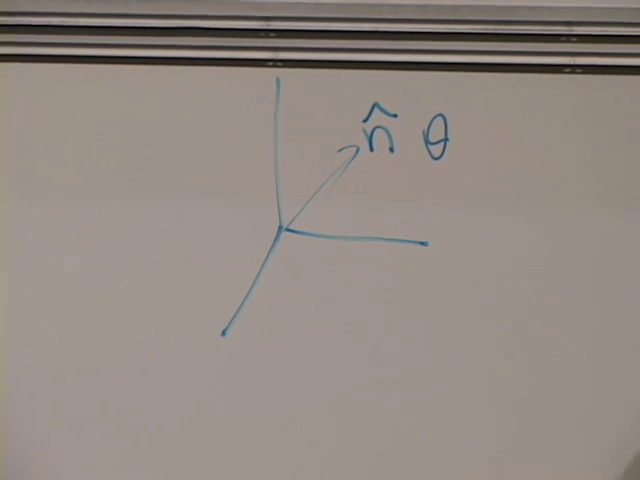
\includegraphics[width=0.58\textwidth]{lecture_03_figure_02.png}
\caption{軸\(\hat{\boldsymbol n}\)與角度\(\theta\)指定一個空間旋轉。}
\lectureframe{00:02:34}
\end{figure}

單位球面上的一個方向需要兩個參數，例如經度和緯度；繞該方向的角度則提供第三個參數。因此，旋轉構成一個三參數族。此處暫不考慮相差\(2\pi\)的角度所造成的整體等同；這裡重要的是局部參數的數目。

軸角描述有些冗餘。反轉軸並同時反轉角度，會得到相同的操作；足夠大的角度也可以對一整圈取模而化簡。這些都不影響以下事實：在恆等旋轉附近，旋轉有三個連續可變的參數。稍後會將這個局部參數數目與矩陣表示中的獨立參數數目相對應。

現在可以依序檢查群的性質：
\begin{enumerate}
\item \emph{封閉性。}連續施行兩個旋轉，結果仍是另一個旋轉。
\item \emph{恆等元。}什麼都不做就是恆等旋轉。
\item \emph{逆元。}繞\(\hat{\boldsymbol n}\)旋轉\(\theta\)，可用繞同一軸旋轉\(-\theta\)來抵消。
\item \emph{結合性。}三個連續旋轉滿足
\[
(R_1R_2)R_3=R_1(R_2R_3).
\]
\end{enumerate}

旋轉不可交換。先繞\(x\)軸旋轉，再繞\(y\)軸旋轉，通常會得到不同於反向次序的取向：
\begin{equation}
R_x(\alpha)R_y(\beta)\ne R_y(\beta)R_x(\alpha).
\end{equation}
若兩個角度都非常小，差異會是二階量，因此無窮小旋轉看起來幾乎可交換。儘管如此，整個群仍是非阿貝爾群。

不必用方程也能檢驗這種不可交換性。拿一本書或一個盒子，在其中一面標上「正面」，先繞\(x\)軸旋轉九十度，再繞\(y\)軸旋轉九十度。回到原來的取向，並反過來施行這兩個旋轉。標記的那一面最後會朝向不同方向。角度較小時，差異較難看出，但並未消失；它從兩個小角度的乘積階開始出現。

\begin{classroomqa}
\audiencequestion{這些旋轉是依序進行，而不是同時進行嗎？\lecturetimestamp{00:04:45}}
\lecturerresponse{是的。群乘法表示先做一個操作，再做另一個操作。這些連續旋轉的次序，正是可能導致不可交換的原因。}
\end{classroomqa}

這是我們遇到的第一個非阿貝爾群。最後要應用的對象不是普通物體的顏色，而是夸克的紅、綠、藍三種色態。這是一個三態的內部系統，其中有趣的變換會混合這三種顏色。普通旋轉則提供了一個熟悉的例子，說明連續群如何透過矩陣作用。

群本身是抽象的。要在物理學中使用它，就必須說明它作用於哪些物件。{表示}會為每個群元素指定一個算符或矩陣，使群元素的乘法由相應矩陣的乘法重現。同一個群可以在不同物理物件上以不同表示作用。向量、自旋一態和自旋二分之一態將作為三個例子。

\section{三維向量表示}

設普通向量的分量為
\begin{equation}
\boldsymbol V=(V_x,V_y,V_z),\qquad V_i,\quad i=1,2,3.
\end{equation}
可以固定座標軸而旋轉物理向量，也可以固定向量而旋轉座標軸。兩種約定有所不同，但無論採用哪一種，分量都會由一個\(3\times3\)矩陣混合。對每一組軸角參數\((\hat{\boldsymbol n},\theta)\)，寫成
\begin{equation}
V_i'=R_{ij}(\hat{\boldsymbol n},\theta)V_j,
\label{eq:l3-vector-rotation}
\end{equation}
其中重複指標表示求和。

重複指標\(j\)是虛指標。方程~\eqref{eq:l3-vector-rotation}明確寫出來就是
\begin{equation}
V_i'=R_{i1}V_1+R_{i2}V_2+R_{i3}V_3
\end{equation}
對每個輸出分量\(i\)都成立。自由指標\(i\)標示正在計算哪個分量；重複指標\(j\)則表示求和，可以改名而不改變方程。分清這兩種角色，就能避免長度保持論證中的大多數指標錯誤。

\begin{figure}[htbp]
\centering
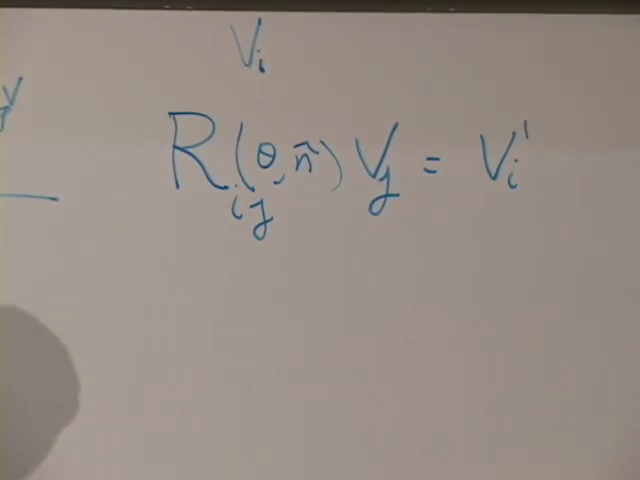
\includegraphics[width=0.68\textwidth]{lecture_03_figure_03.png}
\caption{旋轉矩陣將原向量的分量映射為旋轉後的分量。}
\lectureframe{00:07:41}
\end{figure}

真正的旋轉會保持長度。目前\(V_i\)和\(R_{ij}\)都是實數，因此
\begin{equation}
V_i'V_i'=V_iV_i
\end{equation}
對任意向量都成立。為了導出矩陣條件，以不同的虛指標寫出同一個變換：
\begin{equation}
V_i'=R_{ij}V_j,\qquad V_i'=R_{ik}V_k.
\end{equation}
相乘並對\(i\)求和，得到
\begin{align}
V_i'V_i'
 &=R_{ij}V_jR_{ik}V_k\\
 &=R_{ij}R_{ik}V_jV_k.
\end{align}
對所有\(V\)的取值，這個結果都等於\(V_jV_j\)，而這只有在
\begin{equation}
R_{ij}R_{ik}=\delta_{jk}.
\label{eq:l3-orthogonality-index}
\end{equation}
時才成立。用矩陣記號表示，
\begin{equation}
R^TR=\boldsymbol 1,
\label{eq:l3-orthogonal}
\end{equation}
因此
\begin{equation}
R^{-1}=R^T.
\end{equation}
轉置就是將行與列互換。

為什麼係數必須是\(\delta_{jk}\)？克羅內克{\proseunicodefont δ}在求和時會令\(j=k\)：
\begin{equation}
\delta_{jk}V_jV_k=V_1^2+V_2^2+V_3^2.
\end{equation}
若\(R_{ij}R_{ik}\)不等於\(\delta_{jk}\)，某個方向的長度或某個交叉項\(V_jV_k\)就會改變。由於等式必須對所有可能的向量成立，而不只是對某個特定向量成立，矩陣係數本身就必須等於單位矩陣。

方程~\eqref{eq:l3-orthogonal}是這個實矩陣表示的正交性定義條件。矩陣乘法重現了空間旋轉的乘法結構。這並非旋轉群唯一的表示，只是最容易想像的一種。

逆矩陣關係有直接的幾何意義。要抵消一個旋轉，不必另解矩陣方程，只要交換行與列即可。若\(R_1\)和\(R_2\)代表兩個旋轉，則\(R_2R_1\)代表它們依序作用的結果，而且仍是正交矩陣。因此，矩陣運算保留了幾何上已確立的封閉性、恆等元、逆元與結合性結構。

\section{自旋一與向量表示}

三維表示也會作用於量子態。自旋一粒子有三種可能的自旋投影：
\begin{equation}
m=+1,\quad 0,\quad -1.
\end{equation}
因此，它的自旋態是由三個機率振幅組成的欄向量。旋轉粒子，或改變用來定義自旋軸的磁場方向，都會透過旋轉群的三維表示來混合這三個振幅。

自旋態的數目遵循熟悉的規則\(2s+1\)。自旋零有一個態，自旋二分之一有兩個，自旋一有三個，自旋三分之二有四個。因此，態向量的維度會隨自旋而變。同一個物理旋轉作用於不同的態空間時，必須由不同大小的矩陣表示。

對自旋一粒子，選取基底
\begin{equation}
\lvert 1,+1\rangle,qquad
\lvert 1,0\rangle,qquad
\lvert 1,-1\rangle.
\end{equation}
一個態可寫成
\begin{equation}
\lvert\psi\rangle
=c_{+}\lvert1,+1\rangle+c_0\lvert1,0\rangle+c_{-}\lvert1,-1\rangle.
\end{equation}
旋轉實驗裝置不會產生第四種自旋態，而只會混合三個係數\(c_+,c_0,c_-\)。因此，相應的旋轉算符必須是\(3\times3\)矩陣。

自旋一的表示與普通空間向量遵循相同的變換方式。這就是稱自旋一粒子為\emph{向量粒子}的確切含義：它的三個自旋振幅與向量的三個分量遵循相同的旋轉定律。量子態不必想像成一支實際的箭頭；這裡說的是其分量如何混合。

這種對應並非偶然。三維向量與自旋一態承載的是旋轉群的等價三維表示。{向量粒子}一詞概括了這種變換性質，並不是說量子極化態是藏在粒子內部的一支微小剛性箭頭。

\section{離散與連續對稱性}

在討論自旋二分之一之前，先區分兩大類群會很有幫助。反射是簡單的離散例子：除了恆等操作，還有反射\(P\)；不是翻轉，就是不翻轉。相較之下，相位
\begin{equation}
e^{i\phi}
\end{equation}
會隨\(\phi\)連續變化，空間旋轉也會隨其軸和角度連續變化。這類連續群稱為\emph{李群}，名稱取自Sophus Lie；Lie讀作\emph{Lee}。本章主要關注連續對稱性，但離散對稱性也很重要。

對於包含兩個元素的反射群，
\begin{equation}
P^2=1.
\end{equation}
在\(1\)與\(P\)之間，沒有可連續調整的反射程度。相位群則不同：在\(e^{i\phi_1}\)與\(e^{i\phi_2}\)之間，還有連續無窮多個其他相位。空間旋轉也具有連續性，但與\(U(1)\)不同，旋轉是非阿貝爾的。

自旋零給出旋轉群最簡單的表示。自旋零態在所有旋轉下都不變，因此每個群元素都由一維單位矩陣表示：
\begin{equation}
D^{(0)}(R)=1.
\end{equation}
群本身仍包含無窮多個旋轉；平凡的是旋轉群在自旋零態上的表示。

群與其表示之間的區分至關重要。旋轉群作用於純量時，並不會因此縮減成只有一個元素的群；而是該群的每個元素在那個特定純量態上都由同一個數\(1\)表示。

\section{一般的自旋二分之一態}

自旋二分之一系統有兩個基底態。相對於選定的\(z\)軸，
\begin{equation}
\lvert\uparrow\rangle=
\begin{pmatrix}1\\0\end{pmatrix},
\qquad
\lvert\downarrow\rangle=
\begin{pmatrix}0\\1\end{pmatrix}.
\end{equation}
一般態是二分量旋量：
\begin{equation}
\lvert\psi\rangle=
\begin{pmatrix}\alpha_1\\\alpha_2\end{pmatrix},
\qquad
|\alpha_1|^2+|\alpha_2|^2=1.
\label{eq:l3-spinor}
\end{equation}
其分量為複數。當\((\alpha_1,\alpha_2)=(1,0)\)時，態為自旋向上；當\((0,1)\)時，態為自旋向下。一般的歸一化線性組合，描述自旋沿其他方向極化的狀態。

{向上}和{向下}只有在選定軸之後才有意義。此處選定的軸是\(z\)。不同的測量軸有不同的一對基底態；沿某一軸具有確定向上自旋的態，在另一組基底中通常會呈現為疊加態。旋轉物理自旋或參考座標軸，會相應改變其係數。

兩個複振幅包含四個實參數。歸一化條件去掉一個參數，物理上無關的整體相位再去掉一個，剩下兩個實參數。這恰好是指定球面上一個方向所需的參數數目。研究旋轉時，不必推導\((\alpha_1,\alpha_2)\)與該方向之間的明確對應關係。

整體相位可以略去，因為
\begin{equation}
\begin{pmatrix}\alpha_1\\\alpha_2\end{pmatrix}
\quad\hbox{and}\quad
e^{i\chi}
\begin{pmatrix}\alpha_1\\\alpha_2\end{pmatrix}
\end{equation}
代表同一條物理射線。歸一化固定的是總機率，而非普通歐幾里得空間中的方向。經過這兩種等同識別後，剩下的兩個參數可視為自旋極化方向的極角與方位角。

旋轉自旋後，其態變為
\begin{equation}
\alpha_i'=U_{ij}\alpha_j,
\qquad
\begin{pmatrix}\alpha_1'\\\alpha_2'\end{pmatrix}
=
\begin{pmatrix}
U_{11}&U_{12}\\
U_{21}&U_{22}
\end{pmatrix}
\begin{pmatrix}\alpha_1\\\alpha_2\end{pmatrix}.
\label{eq:l3-spinor-transform}
\end{equation}
因此，空間旋轉在旋量上有一個二維矩陣表示。這個表示具有整體的雙值性，稍後再討論；在局部範圍內，這些矩陣具備下文所需的變換性質。

變換後的二元組\((\alpha_1',\alpha_2')\)必須仍是可能的量子態。因此，關於\(U\)，首先要問的不是它明確的軸角公式，而是它必須滿足什麼條件，才能保持任意輸入旋量的歸一化。

\section{機率守恆與么正矩陣}

旋轉必須將歸一化態映射為另一個歸一化態：
\begin{equation}
\alpha_i^*\alpha_i=\alpha_i'^*\alpha_i'=1.
\end{equation}
代入方程~\eqref{eq:l3-spinor-transform}，得到
\begin{align}
\alpha_i'^*\alpha_i'
 &=(U_{ij}\alpha_j)^*(U_{ik}\alpha_k)\\
 &=\alpha_j^*U_{ij}^*U_{ik}\alpha_k.
\end{align}
因此，對應於實向量的條件是
\begin{equation}
(U^T)^*U=\boldsymbol 1.
\end{equation}
轉置後取複共軛就是厄米共軛：
\begin{equation}
U^\dagger=(U^T)^*,
\end{equation}
所以，保持歸一化的條件為
\begin{equation}
U^\dagger U=\boldsymbol 1.
\label{eq:l3-unitarity}
\end{equation}

與實向量的計算相比，唯一關鍵的差別是多了複共軛。對實向量而言，\(V_iV_i\)是長度；對旋量而言，\(\alpha_i^*\alpha_i\)是機率。為了使機率為實數且非負，必須取複共軛，因此轉置要改為厄米共軛。

方程~\eqref{eq:l3-unitarity}也立刻給出逆矩陣：
\begin{equation}
U^{-1}=U^\dagger.
\end{equation}
因此，逆旋轉也會保持相同的機率範數。和普通旋轉矩陣一樣，么正矩陣的乘積仍是么正矩陣，所以這個表示保留了群乘法結構。

\begin{figure}[htbp]
\centering
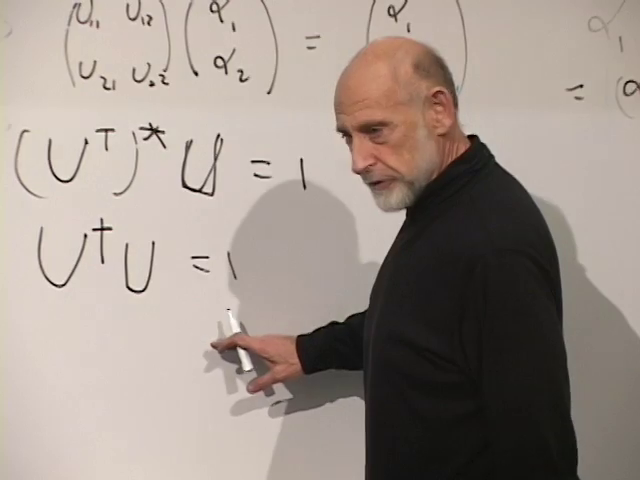
\includegraphics[width=0.62\textwidth]{lecture_03_figure_04.png}
\caption{旋量旋轉矩陣滿足\(U^\dagger U=\boldsymbol 1\)。}
\lectureframe{00:27:41}
\end{figure}

滿足方程~\eqref{eq:l3-unitarity}的矩陣稱為么正矩陣。一般的\(2\times2\)複矩陣有八個實參數。么正條件是一個\(2\times2\)矩陣方程，提供四個獨立的實約束，因此剩下四個參數。空間旋轉只有三個參數。要從整個\(U(2)\)中選出旋轉的旋量表示，還需要一個限制。

也可以將\(U\)的兩個欄視為兩個複向量，從而看出這四個約束：每個欄的範數都必須為一，這提供兩個實條件；兩欄還必須互相正交，這是一個複數條件，也就是兩個實條件。總共四個。\(U(2)\)剩下的第四個參數，最後會證明是整體行列式相位，而非新的空間旋轉。

\section{行列式為一與\texorpdfstring{\(SU(2)\)}{SU(2)}}

額外條件是
\begin{equation}
\det U=1.
\label{eq:l3-det-one}
\end{equation}
此條件與群乘法相容，因為
\begin{equation}
\det(AB)=\det A\,\det B.
\end{equation}
兩個行列式為一的么正矩陣相乘，所得矩陣的行列式仍為一；單位元的行列式也是一。這些矩陣構成一個封閉子群。

逆矩陣也屬於這個子群。若\(\det U=1\)，則
\begin{equation}
\det U^{-1}=\frac{1}{\det U}=1.
\end{equation}
因此，施加行列式為一的條件，不會移除單位元、破壞封閉性或排除逆元。這項條件一致地選出一個少一個連續參數的群。

么正性本身只推出
\begin{equation}
\det(U^\dagger U)=
(\det U)^*\det U
=|\det U|^2=1.
\end{equation}
並不能迫使\(\det U\)等於\(+1\)或\(-1\)。一般么正矩陣的行列式可以是任意相位：
\begin{equation}
\det U=e^{i\phi},
\qquad
\det U^\dagger=e^{-i\phi}.
\end{equation}
條件~\eqref{eq:l3-det-one}固定了原本自由的這個相位，並去掉一個實參數。

\begin{classroomqa}
\audiencequestion{若沒有行列式為一的條件，\(U^\dagger U=\boldsymbol 1\)是否會迫使\(\det U^\dagger\)等於\(\det U\)，或只允許\(+1\)、\(-1\)？\lecturetimestamp{00:31:21}}
\lecturerresponse{不會。兩個行列式互為複共軛；它們可以分別是\(e^{i\phi}\)和\(e^{-i\phi}\)，兩者的乘積為一。特殊么正條件則進一步將兩者都固定為一。}
\end{classroomqa}

么正的\(n\times n\)矩陣構成\(U(n)\)。當\(n=1\)時，么正矩陣就是相位\(e^{i\phi}\)，因此得到\(U(1)\)。行列式為一的子群稱為\emph{特殊么正群}：
\begin{equation}
SU(n)=\{U\in U(n):\det U=1\}.
\end{equation}
二分量旋量由\(SU(2)\)作用；這是一個三參數群。

這個記號同時表明兩項限制：\(U\)表示么正，\(S\)表示特殊，也就是行列式為一。特殊么正群會反覆出現，因為它們既保持複內積，又排除了行列式所帶有的獨立整體相位。

在局部範圍內，\(SU(2)\)具有旋轉自旋二分之一態所需的相同旋轉代數與乘法結構。在整體範圍內，則須記得先前暫緩討論的細節：\(SU(2)\)是普通旋轉群\(SO(3)\)的雙覆蓋，因此\(SU(2)\)中的兩個元素會對應到同一個空間旋轉。\editorialnote{雙覆蓋的表述，精確說明了原文提及但未展開的雙值性。}

\section{無窮小旋轉與泡利矩陣}

\begin{classroomqa}
\audiencequestion{自旋矩陣，也就是泡利矩陣，是如何出現在這個構造中的？\lecturetimestamp{00:33:16}}
\lecturerresponse{當群元素非常接近恆等元時，也就是對應到非常小角度的旋轉時，泡利矩陣便會出現。它們是這些無窮小旋轉的生成元。}
\end{classroomqa}

從
\begin{equation}
U=\boldsymbol 1+\epsilon M+O(\epsilon^2),
\label{eq:l3-small-u-anti}
\end{equation}
開始，其中\(\epsilon\)是實數且很小。於是
\begin{equation}
U^\dagger=\boldsymbol 1+\epsilon M^\dagger+O(\epsilon^2),
\end{equation}
而么正條件給出
\begin{align}
U^\dagger U
 &=\boldsymbol 1+\epsilon(M^\dagger+M)+O(\epsilon^2).
\end{align}
保留至一階可得
\begin{equation}
M^\dagger=-M.
\end{equation}
因此，方程~\eqref{eq:l3-small-u-anti}中的矩陣\(M\)是反厄米矩陣。

這裡只保留\(\epsilon\)的一次項。乘積\(\epsilon^2M^\dagger M\)是二階項，因此略去。這正是在恆等元附近運算的好處：非線性的群條件會轉化為對生成元的線性條件。

更方便的做法是提出一個\(i\)因子：
\begin{equation}
U=\boldsymbol 1+i\epsilon H+O(\epsilon^2).
\label{eq:l3-small-u-herm}
\end{equation}
複共軛會將\(i\)變為\(-i\)，因此
\begin{equation}
U^\dagger=\boldsymbol 1-i\epsilon H^\dagger+O(\epsilon^2).
\end{equation}
現在
\begin{equation}
U^\dagger U
=\boldsymbol 1+i\epsilon(H-H^\dagger)+O(\epsilon^2),
\end{equation}
一階么正條件要求
\begin{equation}
H^\dagger=H.
\end{equation}
提出\(i\)因子後，生成元便是厄米矩陣。

乘上\(i\)並未改變允許的無窮小矩陣，只改變了生成元的命名慣例。物理學通常採用厄米生成元，因為它們的本徵值為實數，且相關可觀測量（例如角動量）也是厄米的。

行列式為一的條件導出無跡條件\editorialnote{口述的行列式展開在下標處略有混淆。正確的線性項是\(A_{11}+A_{22}=\operatorname{tr}A\)；非對角項的乘積則從二階開始。}。對小的\(2\times2\)矩陣\(A\)，
\begin{equation}
\det(\boldsymbol 1+A)
=
\det
\begin{pmatrix}
1+A_{11}&A_{12}\\
A_{21}&1+A_{22}
\end{pmatrix}.
\end{equation}
展開後，
\begin{align}
\det(\boldsymbol 1+A)
 &=(1+A_{11})(1+A_{22})-A_{12}A_{21}\\
 &=1+A_{11}+A_{22}+O(A^2)\\
 &=1+\operatorname{tr}A+O(A^2).
\end{align}
將此結果用於\(A=i\epsilon H\)，得到
\begin{equation}
\det U=1+i\epsilon\,\operatorname{tr}H+O(\epsilon^2).
\end{equation}
因此，\(\det U=1\)要求
\begin{equation}
\operatorname{tr}H=0.
\end{equation}
跡條件恰好去掉與單位矩陣成正比的生成元。一般的厄米\(2\times2\)矩陣有四個實參數：兩個實數對角元素，以及一個複數非對角元素。跡條件固定其中一個實數組合，於是剩下三個參數。這與無窮小空間旋轉可選的三個旋轉軸相符。

因此，\(SU(2)\)的無窮小生成元是無跡厄米\(2\times2\)矩陣。三個泡利矩陣構成一組基底：
\begin{equation}
\begin{aligned}
\sigma_x&=
\begin{pmatrix}0&1\\1&0\end{pmatrix},
&
\sigma_y&=
\begin{pmatrix}0&-i\\i&0\end{pmatrix},
\\[0.4em]
\sigma_z&=
\begin{pmatrix}1&0\\0&-1\end{pmatrix}.
\end{aligned}
\end{equation}
每個生成元都可以寫成
\begin{equation}
H=a_x\sigma_x+a_y\sigma_y+a_z\sigma_z.
\end{equation}
繞\(x\)軸的小旋轉對應到\(\sigma_x\)；繞\(y\)軸的小旋轉對應到\(\sigma_y\)；繞其他軸旋轉則對應到相應的線性組合。在\(\hbar=1\)的單位制下，自旋算符為
\begin{equation}
S_i=\frac{\sigma_i}{2}.
\end{equation}

例如，位於\(x\)軸與\(y\)軸正中間的旋轉軸，其生成元正比於
\begin{equation}
\frac{\sigma_x+\sigma_y}{\sqrt2}.
\end{equation}
係數向量\((a_x,a_y,a_z)\)的方向決定旋轉軸；其大小與\(\epsilon\)共同決定小角度。這便是角動量對易關係中出現的自旋矩陣，與有限旋轉算符之間的關聯。特別是，
\begin{equation}
[S_x,S_y]=iS_z
\end{equation}
以及循環置換所得的關係，表達了前面從幾何上看到的不可交換性。標準的有限旋轉可由無窮小生成元取指數得到\editorialnote{指數形式的有限旋轉公式，是無窮小構造的標準延伸；原文只推導了生成元條件及其泡利矩陣基底。}，
\begin{equation}
U(\hat{\boldsymbol n},\theta)
=\exp\left(-\frac{i\theta}{2}\,
\hat{\boldsymbol n}\cdot\boldsymbol\sigma\right).
\end{equation}
\section{三態色空間}

表示的組合可以稍後再談。現在先離開空間自旋，回到夸克的色。夸克仍具有自旋二分之一，但色是另一個獨立的三態自由度：
\begin{equation}
\lvert r\rangle,\qquad
\lvert g\rangle,\qquad
\lvert b\rangle.
\end{equation}
一般的色態為
\begin{equation}
\begin{aligned}
\lvert q\rangle_{\mathrm{color}}
={}&
\alpha_r\lvert r\rangle
+\alpha_g\lvert g\rangle
+\alpha_b\lvert b\rangle,
\\
&|\alpha_r|^2+|\alpha_g|^2+|\alpha_b|^2=1.
\end{aligned}
\end{equation}
也可以寫成
\begin{equation}
q=
\begin{pmatrix}
\alpha_r\\
\alpha_g\\
\alpha_b
\end{pmatrix}.
\end{equation}
在選定的色基底下，這些係數模平方分別是測得紅、綠、藍色的機率。同樣的三分量表示法也可以將三個夸克場算符排成一個欄向量：
\begin{equation}
\psi=
\begin{pmatrix}
\psi_r\\
\psi_g\\
\psi_b
\end{pmatrix}.
\end{equation}

概念上必須區分自旋與色。自旋標籤描述態在物理空間旋轉下如何變換；色標籤描述態在不旋轉實驗室的內部對稱性下如何變換。夸克態同時帶有這兩種標籤；目前為了聚焦於色，暫不顯示自旋自由度。

將三個場算符排成一個欄向量，不只是為了方便記錄；這讓我們能用一個矩陣方程表達對稱性。變換可以將紅色場變為紅、綠、藍色場的線性組合，就如空間旋轉會將一個向量分量變為其他分量的線性組合。

可以先想像交換兩種顏色的離散變換。更大的對稱群還包含三種顏色之間的連續混合。簡單的交換矩陣可能需要乘上一個相位，才能使行列式等於一；如此一來，這種交換就會包含在特殊么正群中。

對於兩個基底態，直接交換兩者可表示為
\begin{equation}
X=
\begin{pmatrix}0&1\\1&0\end{pmatrix},
\qquad
\det X=-1.
\end{equation}
將整個矩陣乘以\(i\)後，得到
\begin{equation}
\det(iX)=i^2\det X=1.
\end{equation}
因此，只要相位選得恰當，離散交換就能成為較大連續群中的一個特定元素。

\begin{classroomqa}
\audiencequestion{只交換兩個基底態的矩陣，其行列式對\(SU(2)\)而言是否不合要求？\lecturetimestamp{00:43:46}}
\lecturerresponse{直接交換的行列式為\(-1\)。乘上適當的\(i\)因子，就能得到行列式為一的代表矩陣，因此這種交換可以包含在連續的特殊么正變換之中。}
\end{classroomqa}

\section{\texorpdfstring{\(SU(3)\)}{SU(3)}與八個色生成元}

連續的色變換為
\begin{equation}
\begin{aligned}
q'&=Uq,
&
U^\dagger U&=\boldsymbol 1,
\\
\det U&=1,
&
U&\in SU(3).
\end{aligned}
\label{eq:l3-su3-action}
\end{equation}
其數學形式與用於旋量的特殊么正構造相同，但此處\(U\)是\(3\times3\)。這不是物理空間的旋轉，而是內部色空間中的旋轉。

么正性會保持色態的歸一化：
\begin{equation}
q^\dagger q
=|\alpha_r|^2+|\alpha_g|^2+|\alpha_b|^2.
\end{equation}
行列式為一則排除了連續混合中的共同\(U(1)\)相位方向。所得矩陣可以進行簡單交換、改變相對相位，也可以形成真正的連續疊加，同時仍屬於同一個封閉群。

參數數目可以直接算出。一個\(3\times3\)複矩陣有九個複數元素，也就是十八個實參數。矩陣方程\(U^\dagger U=\boldsymbol 1\)施加九個實條件；行列式為一再去掉一個參數：
\begin{equation}
\dim SU(3)=18-9-1=8.
\end{equation}
因此，\(SU(3)\)有八個獨立的無窮小生成元。

也可以透過\(U\)的欄來理解這九個么正條件。三個複數欄向量各自都必須具有單位範數，而且每一對都必須互相正交。這些條件從原有的十八個實參數中去掉九個；行列式的相位再去掉第十個，剩下八個。這是三態情形下，\(SU(2)\)的\(8-4-1=3\)參數計數的對應情形。

八這個數字的出現，與最終得到八種膠子，是同一個事實所致。說膠子之所以不是九種，是因為行列式限制移除了一個方向，這只是一種助記說法。更精確地說，九個色－反色矩陣可分解為一個與單位矩陣成正比的色單態方向，以及八個無跡方向。這八個無跡生成元構成 QCD 膠子所承載的伴隨色結構。\editorialnote{單態加八重態的表述，是對原文刻意採用的啟發式行列式說法所作的標準精確詮釋；規範場的構造留待後續討論。}

此時，八種膠子與前述結果的關聯只是提示，還不是完整的推導。要得到規範粒子，必須將色對稱性提升為局域對稱性，並確定補償場。參數計數已經表明，在\(SU(3)\)色變換中，有八個獨立方向可使變換從單位元開始偏離。

\section{色對稱性對 QCD 的約束}

基本的對稱性敘述是：物理定律在方程式~\eqref{eq:l3-su3-action}所示的色變換下保持不變。這是量子色動力學的核心內部對稱性。色分量的混合在形式上類似於自旋向上與自旋向下振幅的混合；而那些旋量變換又與空間方向的旋轉相關，但這三種空間不可混為一談。

稱色為一種對稱性，意指改變色基底不會改變物理預測。紅、綠、藍是三個基底向量的方便稱呼，並非三種可觀測的顏料。對色分量同時施行\(SU(3)\)旋轉，必須使定律的形式保持不變。這種不變性並非可有可無的美學特徵，而是 QCD 的組織原則。

對稱性會限制拉格朗日量。在先前的\(U(1)\)例子中，對共同相位變換的不變性，限制了允許出現的項，使其包含場與其共軛場的平衡因子。在 QCD 中，每一項同樣都必須在\(SU(3)\)色變換下保持不變。這項要求會影響相互作用、守恆量，以及膠子場的形式。

假設某個候選項帶有一個未縮併的色指標。在方程式~\eqref{eq:l3-su3-action}所示的變換下，該指標會旋轉，因此此項本身無法保持不變。允許的項必須將色指標縮併成不變組合，或使用變換能補償這項變化的規範場。這就是對稱性原理的實際作用：它排除任意耦合，並規範剩餘相互作用的形式。

QCD 的完整構造還需要進一步處理：必須允許色變換隨位置改變，並由規範場補償這種局域變化。\editorialnote{將色對稱性局域化，是全域\(SU(3)\)討論在規範理論中的標準延伸；本講稿並未展開這部分。}這部分內容留待下一階段。目前，基本結構已經建立：色三重態受到具有八個生成元的三態特殊酉對稱性作用。

目前所需的群論計算已經完成。我們從能在普通空間中描繪的旋轉出發，進而討論作用於向量和旋量的矩陣，再把同樣的邏輯運用到內部色空間。下一步可以在已有數學架構的基礎上回到粒子物理，而不必讓形式體系一次承載全部物理內容。
\chapter{色表示、強子與禁閉}

\paragraph{簡短的開場插曲。}
回到群論之前，容我先做一次不太要臉的商業宣傳。\emph{《黑洞戰爭》}講述了我與 Stephen Hawking 之間一場漫長的爭論：黑洞是否會摧毀量子資訊。書中也記錄了理論物理學家特有的一些殘酷玩笑：不只有薛丁格的貓，還有 Susskind 的魚，以及牠們不幸掉進馬桶的遭遇。這項任務完成後，我們回到 Alice 和 Bob。Alice 仍然很苦惱，因為 Bob 還在逼她學群論。

\lectureoverview{對稱性藉由作用於態而具有物理意義。我們先從旋轉談起，介紹表示與生成元，再將這套建構方式用於色\(SU(3)\)。色表示可以組合成強子，而其動力學則說明了為何從未觀測到孤立的色。}

\section{群及其作用對象}

每次討論對稱性，都包含兩個概念。第一個是抽象群：一組具有乘法法則、單位元與逆元的運算。第二個是這些運算所作用的對象。兩者可以區分，但在物理學中無法分開。對稱性之所以重要，是因為它會變換物理態、場、座標或可觀測量。

\begin{classroomqa}
\audiencequestion{群既被描述為抽象的乘法表，也被描述為作用於物理對象的矩陣。這兩個部分可以分開嗎？
\lecturetimestamp{00:01:58}}
\lecturerresponse{它們是不同層次的描述，但彼此完全相關。旋轉作為一種抽象運算，在我們指定它要旋轉什麼之前就已存在。接著，物理學要探討的是，同一個運算如何作用於特定系統相關的態與物理量。矩陣提供這種具體的作用，同時保留抽象的乘法法則。}
\end{classroomqa}

空間旋轉是最清楚的例子。在古典力學中，同一個旋轉可以作用於粒子的座標、磁鐵的方向，或任何其他向量。在量子力學中，態屬於線性向量空間，因此旋轉由作用於該空間的線性算符表示。若\(g\)表示抽象群元素，而\(D(g)\)表示其矩陣代表，則一致性要求
\begin{equation}
D(g_1g_2)=D(g_1)D(g_2),
\qquad
D(e)=\boldsymbol 1.
\end{equation}
矩陣不必與抽象運算長得相同，但矩陣的乘法必須重現群的乘法。
\editorialnote{同態方程明確寫出源文以文字說明的群乘法與矩陣乘法之間的對應關係。}

矩陣的維度由態空間決定，而不單由抽象群決定。若只考慮單一電子的自旋，就有兩種彼此正交的可能態：自旋向上與自旋向下；因此，態是二分量列向量。旋轉於是由\(2\times2\)矩陣表示。對兩個自旋為二分之一的物體，基底包含四個態，
\begin{equation}
\ket{\uparrow\uparrow},\qquad
\ket{\uparrow\downarrow},\qquad
\ket{\downarrow\uparrow},\qquad
\ket{\downarrow\downarrow},
\end{equation}
因此，旋轉在組合空間上的作用是四維的。

熟悉的序列如下：
\begin{equation}
\begin{array}{c|c|c}
\text{spin} & \text{number of states} & \text{matrix dimension}\\
\hline
0 & 1 & 1\times1\\
\frac12 & 2 & 2\times2\\
1 & 3 & 3\times3\\
\frac32 & 4 & 4\times4
\end{array}
\end{equation}
依此類推。自旋為零的態構成平凡表示：任何旋轉都不改變它。一乘一矩陣就是\(1\)。自旋為一的態有三個分量，其旋轉矩陣就是熟悉的三維向量旋轉。一般而言，自旋\(j\)的表示有\(2j+1\)個態。

表示也可以是無限維的。若我們描述電子完整的軌道運動，而不只考慮它的自旋，態就包含每個位置的振幅，或等價地，包含每個動量的振幅。此時，旋轉算符作用於無限維的波函數空間。因此，同一個抽象旋轉群可以有平凡、二維、三維與無限維表示。從自旋轉而討論色時，我們會再次用到這個事實。

\section{為什麼自旋旋轉屬於特殊酉群}

現在回到單一電子的自旋，並略去其軌道運動。旋轉以一個\(2\times2\)酉矩陣\(U\)表示，
\begin{equation}
U^\dagger U=\boldsymbol 1,
\qquad
U^{-1}=U^\dagger.
\label{eq:l4-unitarity}
\end{equation}
逆變換必須還原原來的旋轉，而酉性會保留範數，因而保留所有機率。

一般的\(2\times2\)複矩陣含有四個複數元素，也就是八個實參數。方程式~\eqref{eq:l4-unitarity}施加四個獨立的實條件，剩下四個參數。普通的空間旋轉只有三個參數：兩個用來選擇旋轉軸，一個用來選擇旋轉角。因此，這個酉矩陣多了一個相位。還需要加上以下限制：
\begin{equation}
\det U=1.
\label{eq:l4-det-one}
\end{equation}
參數計數於是為
\begin{equation}
8-4-1=3.
\end{equation}

行列式為一的條件在矩陣乘法下保持不變，因為
\begin{equation}
\det(AB)=\det A\,\det B.
\end{equation}
若兩個矩陣的行列式皆為一，其乘積的行列式也為一。這個條件也與酉性相容。對方程式~\eqref{eq:l4-unitarity}兩邊取行列式，得到
\begin{equation}
1=\det(U^\dagger U)
=\det(U^\dagger)\det U
=(\det U)^*\det U.
\end{equation}
因此，酉矩陣的行列式位於單位圓上：
\begin{equation}
\det U=e^{i\phi}.
\end{equation}

\begin{classroomqa}
\audiencequestion{酉性是否要求行列式為實數？
\lecturetimestamp{00:12:10}}
\lecturerresponse{不要求。酉性只要求模長為一。行列式可以是任意純相位\(e^{i\phi}\)。對二維矩陣而言，將\(U\)乘上\(e^{-i\phi/2}\)，即可消去共同相位，得到行列式為一的矩陣。}
\end{classroomqa}

確實，若
\begin{equation}
V=e^{-i\phi/2}U,
\end{equation}
則\(V\)仍然是酉矩陣，而且
\begin{equation}
\det V=e^{-i\phi}\det U=1.
\end{equation}
行列式為一的酉矩陣構成\(SU(2)\)。

有一點需要留意。很容易把\(SU(2)\)說成就是三維空間的旋轉群，但兩者之間是二對一的對應。矩陣\(U\)與\(-U\)對旋量的作用不同，卻對應到普通向量的同一個旋轉。因此
\begin{equation}
SU(2)/\{\boldsymbol 1,-\boldsymbol 1\}\simeq SO(3).
\end{equation}
在目前的討論中，重要的是局部乘法結構與三個生成元；雙重覆蓋則說明了自旋為二分之一的粒子為何具有二值旋轉性質。

\section{無窮小變換與其生成元}

有限旋轉可以由許多極小旋轉組成。接近單位元的群元素稱為無窮小元素。在連通群中，只要知道所有無窮小方向，就足以透過反覆相乘重建有限變換。對物理學更重要的是，生成這些無窮小變換的算符，就是與對稱性相關的守恆量。

將接近單位元的元素寫成
\begin{equation}
U=\boldsymbol 1+i\epsilon T,
\qquad |\epsilon|\ll1.
\label{eq:l4-infinitesimal-u}
\end{equation}
因子\(i\)是為了方便而採用的慣例。將此式代入酉性條件，並略去\(\epsilon^2\)階的項，可得
\begin{align}
(\boldsymbol 1+i\epsilon T)
(\boldsymbol 1-i\epsilon T^\dagger)&=\boldsymbol 1,
\\
i\epsilon(T-T^\dagger)&=0,
\\
T&=T^\dagger.
\label{eq:l4-hermitian-generator}
\end{align}
生成元是厄米算符，正如量子力學中的可觀測量必須具備的性質。

\begin{figure}[htbp]
\centering
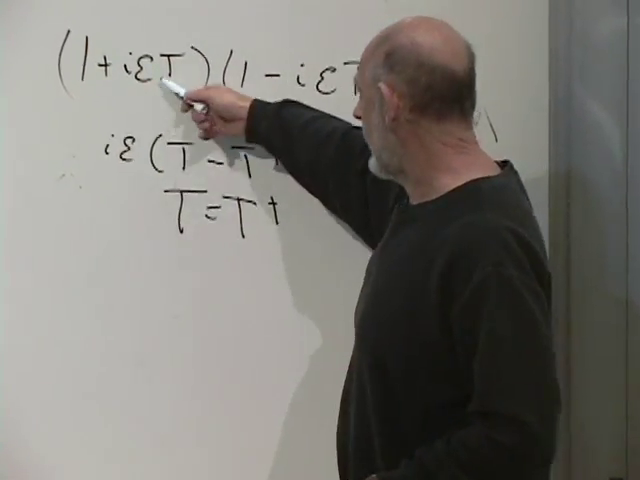
\includegraphics[width=0.62\textwidth]{lecture_04_figure_03.png}
\caption{接近單位元時的酉性計算，結果為\(T=T^\dagger\)。}
\lectureframe{00:23:28}
\end{figure}

空間旋轉有三個線性獨立的生成元，因為有三個獨立的無窮小旋轉軸。繞任意方向的微小旋轉，都可以由繞\(x\)、\(y\)和\(z\)的微小旋轉組成。相應的生成元是角動量算符\(J_x,J_y,J_z\)。它們的對易關係體現了旋轉的不對易性：
\begin{equation}
[J_i,J_j]=i\epsilon_{ijk}J_k.
\label{eq:l4-angular-momentum-algebra}
\end{equation}
反覆施行無窮小旋轉，便能構成有限旋轉。

我們已經使用酉性，但還沒有用到行列式為一的條件。對任意小矩陣\(m\)，
\begin{equation}
\det(\boldsymbol 1+\epsilon m)
=1+\epsilon\,\operatorname{tr}m+O(\epsilon^2).
\label{eq:l4-det-expansion}
\end{equation}

\begin{figure}[htbp]
\centering
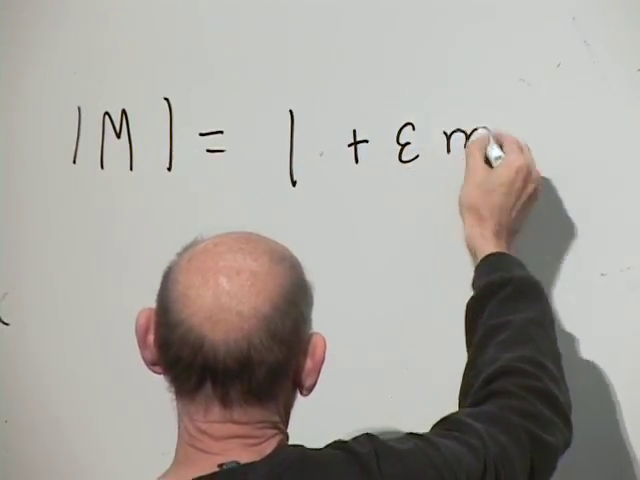
\includegraphics[width=0.62\textwidth]{lecture_04_figure_02.png}
\caption{黑板上推導行列式的一階展開。}
\lectureframe{00:21:51}
\end{figure}

將方程式~\eqref{eq:l4-det-expansion}應用於
方程式~\eqref{eq:l4-infinitesimal-u}，可得
\begin{equation}
\det U
=1+i\epsilon\,\operatorname{tr}T+O(\epsilon^2).
\end{equation}
因此，特殊酉條件要求
\begin{equation}
\operatorname{tr}T=0.
\label{eq:l4-traceless-generator}
\end{equation}
\(SU(2)\)的生成元正是無跡厄米\(2\times2\)矩陣。這個向量空間的維度為三。泡利矩陣構成一組標準基底：
\begin{equation}
\begin{aligned}
\sigma_x&=
\begin{pmatrix}0&1\\1&0\end{pmatrix},
&
\sigma_y&=
\begin{pmatrix}0&-i\\i&0\end{pmatrix},
\\[0.4em]
\sigma_z&=
\begin{pmatrix}1&0\\0&-1\end{pmatrix}.
\end{aligned}
\end{equation}
對自旋為二分之一的表示，可以取\(J_i=\sigma_i/2\)。因此，繞\(\hat{\boldsymbol n}\)旋轉角度\(\theta\)的有限旋轉為
\begin{equation}
U(\hat{\boldsymbol n},\theta)
=\exp\!\left(-i\theta\,
\hat{\boldsymbol n}\cdot\boldsymbol\sigma/2\right).
\end{equation}
\editorialnote{有限指數式是無窮小生成元討論的標準延伸。源文著重於反覆施行小旋轉，沒有明確寫出這個公式。}

\begin{classroomqa}
\audiencequestion{所以有三個線性獨立的無跡厄米\(2\times2\)矩陣？
\lecturetimestamp{00:24:07}}
\lecturerresponse{是的，就是三個泡利矩陣。對\(3\times3\)特殊酉矩陣，相應的數目是八；一組慣用基底是八個 Gell-Mann 矩陣。}
\end{classroomqa}

\begin{classroomqa}
\audiencequestion{這個「八」，和八重道以及八種膠子中的``八''是同一個意思嗎？
\lecturetimestamp{00:24:43}}
\lecturerresponse{數學上都涉及\(SU(3)\)表示論，但必須說清楚是哪一種\(SU(3)\)對稱性在作用。歷史上的八重道味對稱性不是色\(SU(3)\)。八種膠子則屬於色\(SU(3)\)的伴隨表示。}
\end{classroomqa}

\section{從 SU(2) 到色 SU(3)}

現在將矩陣從\(2\times2\)擴大到\(3\times3\)。一般的複數\(3\times3\)矩陣有九個複數元素，也就是十八個實參數。條件\(U^\dagger U=\boldsymbol 1\)提供九個實約束，而\(\det U=1\)再去掉一個參數。因此
\begin{equation}
18-9-1=8.
\end{equation}
有八個獨立的無窮小方向，以及八個無跡厄米生成元。與\(SU(2)\)不同，這個群不是普通三維空間的旋轉群，而是作用於色的內部對稱性。

在把這些表示指定給夸克之前，先回顧複合表示如何形成。將兩個自旋為二分之一的系統組合起來，並忽略它們的軌道運動。共有四個乘積態，但旋轉不會不可約地混合這四個態。其中三個組合按自旋一變換：
\begin{align}
\ket{1,1}&=\ket{\uparrow\uparrow},\\
\ket{1,0}&=\frac{1}{\sqrt2}
(\ket{\uparrow\downarrow}+\ket{\downarrow\uparrow}),\\
\ket{1,-1}&=\ket{\downarrow\downarrow},
\end{align}
第四個則按自旋零變換：
\begin{equation}
\ket{0,0}=\frac{1}{\sqrt2}
(\ket{\uparrow\downarrow}-\ket{\downarrow\uparrow}).
\end{equation}
因此
\begin{equation}
\boldsymbol 2\otimes\boldsymbol 2
=\boldsymbol 3\oplus\boldsymbol 1.
\label{eq:l4-two-spin-decomposition}
\end{equation}
對齊的態給出三重態中\(m=\pm1\)的成員；對稱的零投影態補足三重態，而反對稱組合則是單態。這就是角動量相加以及色表示組合的一般原理。

每當兩個自旋為二分之一的自由度耦合，都會出現同樣的單態--三重態區分。在氫原子中，電子與質子的自旋形成超精細單態和三重態。正氫與仲氫的兩個質子，其核自旋也遵循相同的表示論；這裡所指的是\(H_2\)分子。
\editorialnote{源文在提到氫原子中的質子--電子自旋時，使用了``正氫與仲氫''。數學上的分解是正確的；為求精確，此處區分了分子與原子的名稱。}

\subsection{三重態與反三重態}

單一夸克有三個色振幅。在選定的基底中，可寫成
\begin{equation}
q=
\begin{pmatrix}
q_r\\q_g\\q_b
\end{pmatrix},
\qquad
q'=Uq,
\qquad U\in SU(3).
\label{eq:l4-quark-triplet}
\end{equation}
這三個分量可以是單一夸克的態振幅，也可以是分別產生紅、綠、藍夸克的三個場算符。群會混合這三個分量。原本為紅色的態，經過色變換後，通常會成為紅、綠、藍的疊加態。這個基本的三維表示稱為\(\boldsymbol 3\)。

對反夸克而言，群透過夸克表示的複共軛表示作用。對方程式~\eqref{eq:l4-quark-triplet}取複共軛，得到
\begin{equation}
\bar q'=U^*\bar q.
\end{equation}
這個表示記作\(\bar{\boldsymbol 3}\)。與\(U(1)\)的類比很直接：若電子場獲得\(e^{i\theta}\)，正電子場便獲得\(e^{-i\theta}\)。夸克與反夸克的色變換，是這種共軛配對在非阿貝爾情形下的版本。

在單位元附近，若
\begin{equation}
U=\boldsymbol 1+i\epsilon T,
\end{equation}
則
\begin{equation}
U^*=\boldsymbol 1-i\epsilon T^*.
\end{equation}
因此，反三重態的生成元是\(-T^*\)，也就是帶有相反符號的共軛生成元。這就是反夸克帶有相反色荷的精確含義。

\begin{classroomqa}
\audiencequestion{在\(SU(2)\)的情況下，複共軛表示會如何？
\lecturetimestamp{00:36:19}}
\lecturerresponse{\(SU(2)\)二重態是特殊情況：經過一個涉及反對稱 epsilon 張量的固定基底變換後，其複共軛表示與原二重態等價。對\(SU(3)\)而言，\(\boldsymbol 3\)與\(\bar{\boldsymbol 3}\)則是真正不等價的表示。}
\end{classroomqa}
\editorialnote{\(SU(2)\)基本表示在數學上精確的術語是「偽實」，而非「實」。這段回答保留了源文要表達的區別，同時修正了術語。}

\section{色表示的組合}

符號\(\otimes\)並非表示將旁邊寫出的數字作普通乘法，而是表示組合兩個態空間。所得的張量積空間接著可重新分解為幾個部分；在群作用下，這些部分彼此不會混合。

\subsection{兩個夸克：\texorpdfstring{\(\boldsymbol 3\otimes\boldsymbol 3\)}{3 x 3}}

兩個夸克共有九個色基底態：紅--紅、紅--綠、紅--藍，以及其餘六種有序配對。將兩個色指標分成對稱部分與反對稱部分。對稱部分有六個獨立分量，反對稱部分有三個。在\(SU(3)\)下，
\begin{equation}
\boldsymbol 3\otimes\boldsymbol 3
=\boldsymbol 6\oplus\bar{\boldsymbol 3}.
\label{eq:l4-three-times-three}
\end{equation}

\begin{figure}[htbp]
\centering
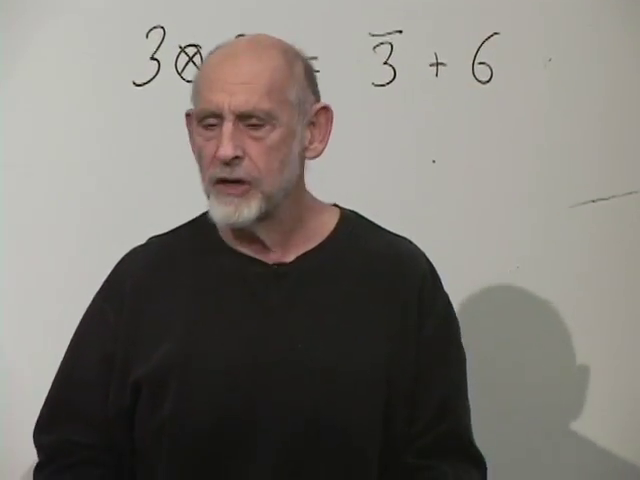
\includegraphics[width=0.68\textwidth]{lecture_04_figure_04.png}
\caption{兩個夸克的乘積分解為反三重態與六重態。}
\lectureframe{00:39:33}
\end{figure}

反三重態可以透過不變 epsilon 張量與兩個夸克指標縮併，明確表示為
\begin{equation}
(qq)^k_{\bar 3}
=\frac{1}{\sqrt2}\epsilon^{kij}q_iq_j.
\end{equation}
這個對象有三個分量，變換方式與反夸克相同。六種對稱組合構成六重態。這並不是說兩個夸克在動力學上變成反夸克，而是說其色波函數中的一個部分，具有與反夸克相同的變換律。

\subsection{一個夸克與一個反夸克：\texorpdfstring{\(\boldsymbol 3\otimes\bar{\boldsymbol 3}\)}{3 ⊗ 反3}}

夸克--反夸克色態可以視為一個\(3\times3\)矩陣\(M_i{}^j=q_i\bar q^j\)。每個這樣的矩陣都可以唯一分解為跡部分與無跡部分：
\begin{equation}
M=\frac{\operatorname{tr}M}{3}\boldsymbol 1
+\left(M-\frac{\operatorname{tr}M}{3}\boldsymbol 1\right).
\end{equation}
跡部分是單一的不變分量，無跡部分則有八個分量。因此
\begin{equation}
\boldsymbol 3\otimes\bar{\boldsymbol 3}
=\boldsymbol 1\oplus\boldsymbol 8.
\label{eq:l4-three-times-threebar}
\end{equation}
單態的形式如下，差一個歸一化因子：
\begin{equation}
\ket{1}_{q\bar q}
=\frac{1}{\sqrt3}
(\ket{r\bar r}+\ket{g\bar g}+\ket{b\bar b}).
\end{equation}
它是不變的，因此不會變換成其他態。其餘八個線性組合會彼此混合，構成伴隨表示；八個生成元也在同一表示中變換。

\subsection{三個夸克}

將第三個夸克與方程式~\eqref{eq:l4-three-times-three}所示的分支組合。反三重態分支給出
\begin{equation}
\bar{\boldsymbol 3}\otimes\boldsymbol 3
=\boldsymbol 1\oplus\boldsymbol 8,
\end{equation}
所以三夸克乘積包含一個單態。完整分解為
\begin{equation}
\boldsymbol 3\otimes\boldsymbol 3\otimes\boldsymbol 3
=\boldsymbol 1\oplus\boldsymbol 8\oplus\boldsymbol 8
\oplus\boldsymbol{10}.
\label{eq:l4-three-quark-full}
\end{equation}
色單態是完全反對稱的紅--綠--藍組合：
\begin{equation}
\ket{1}_{qqq}
=\frac{1}{\sqrt6}\epsilon^{ijk}\ket{q_iq_jq_k}.
\label{eq:l4-baryon-singlet}
\end{equation}
只要有兩個指標相同，\(\epsilon^{ijk}\)就會消失。因此，每個非零項都包含一個紅夸克、一個綠夸克和一個藍夸克；交換指標時，符號會交替。

\begin{classroomqa}
\audiencequestion{非單態組合只是出現機率很低，所以可以忽略它們的機率嗎？
\lecturetimestamp{00:46:02}}
\lecturerresponse{不可以。關鍵在於能量，而不是機率很小。孤立的非單態會使色場延伸至任意遠處；在禁閉區域中，這需要無界大的能量。下文會進一步說明這個說法背後的動力學。}
\end{classroomqa}

\subsection{膠子八重態}

膠子場的變換方式與方程式~\eqref{eq:l4-three-times-threebar}中的八重態相同。就色而言，它帶有一個三重態指標和一個反三重態指標，並扣除單態跡部分。概略地說，
\begin{equation}
q\sim\boldsymbol 3,
\qquad
\bar q\sim\bar{\boldsymbol 3},
\qquad
G\sim\boldsymbol 8.
\end{equation}
這些符號表示變換律；粒子並不等同於數字三或八。

第九種夸克--反夸克色組合與單位矩陣成正比，構成一個單態，不會與八重態混合。因此，省略這個單態在數學上是自洽的：\(SU(3)\)規範場是無跡的，含有八個分量；\(U(3)\)規範場則有九個分量。

\begin{classroomqa}
\audiencequestion{為什麼自然界省略了額外的單態膠子？
\lecturetimestamp{00:49:00}}
\lecturerresponse{直接的群論答案是：單態屬於獨立的不變子空間，因此即使不包含單態，八重態也能構成封閉的表示。此處不推導選擇\(SU(3)\)而非\(U(3)\)的更深層原因；這是從 QCD 現象學推知的規範結構之一。}
\end{classroomqa}

\section{色單態與強子}

強相互作用中自由且質量有限的粒子都是色單態。這不表示夸克或膠子並不存在，而是表示它們不會以孤立的漸近粒子形式出現。形成單態的基本模式如下：
\begin{equation}
qqq,
\qquad
q\bar q,
\qquad
GG\ \text{and higher gluonic products}.
\end{equation}
它們依序形成重子、介子與膠球。若干已無色的對象組合起來，當然仍然無色，因此還可以由這些成分構成更複雜的多強子態。

\begin{classroomqa}
\audiencequestion{三夸克單態與夸克--反夸克單態各稱為什麼？膠子也能組成單態嗎？
\lecturetimestamp{00:51:38}}
\lecturerresponse{三夸克單態稱為重子；夸克--反夸克單態稱為介子。膠子也可以組合成色單態。這類強相互作用態中最簡單的稱為膠球，參與組合的膠子也可以多於兩個。}
\end{classroomqa}

三個自旋為二分之一的夸克，總自旋必為半整數；不過，軌道角動量會影響最後得到哪個半整數。夸克--反夸克介子的自旋為整數。純膠子的膠球自旋也為整數。

對兩個膠子而言，黑板上的第一個陳述只是在計數：
\begin{equation}
8\times8=1+63.
\end{equation}
總共有六十四個色態，其中一個組合是單態，其餘六十三個屬於非單態子空間。

\begin{figure}[htbp]
\centering
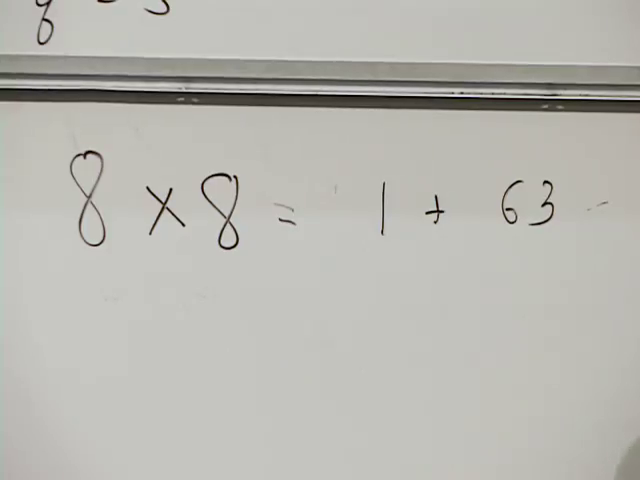
\includegraphics[width=0.68\textwidth]{lecture_04_figure_05.png}
\caption{黑板上的雙膠子態計數：六十四個態中有一個單態。}
\lectureframe{00:53:44}
\end{figure}

完整的不可約分解為
\begin{equation}
\boldsymbol 8\otimes\boldsymbol 8
=\boldsymbol 1\oplus\boldsymbol 8_S\oplus\boldsymbol 8_A
\oplus\boldsymbol{10}\oplus\overline{\boldsymbol{10}}
\oplus\boldsymbol{27}.
\label{eq:l4-eight-times-eight}
\end{equation}
維度相加無誤：
\begin{equation}
1+8+8+10+10+27=64.
\end{equation}
兩個八重態是不同的不變子空間；其中一個在交換兩個伴隨表示因子時對稱，另一個則反對稱。單態則是可以形成膠球態的雙膠子色道。
\editorialnote{黑板上最初只寫出\(8\times8=1+63\)。隨後的課堂問答提供了列出的不可約表示維度；此處依標準\(SU(3)\)記號補上橫線與對稱性標記。}

\subsection{為什麼可觀測到的電荷是整數}

夸克電荷分為兩種：
\begin{equation}
Q_{\mathrm{up\text{-}like}}=+\frac23,
\qquad
Q_{\mathrm{down\text{-}like}}=-\frac13.
\end{equation}
因此三個夸克的總電荷必為整數：\(-1,0,+1,\text{ or }+2\)，取決於其中有多少個是上型夸克。夸克與反夸克組成的態，電荷也會是\(0\)或\(\pm1\)。膠子不帶電。因此，由已觀測到的夸克表示所構成的基本色單態，電荷都是整數，儘管其中的組分帶有分數電荷。

\begin{classroomqa}
\audiencequestion{奇異夸克帶多少電荷？
\lecturetimestamp{00:56:08}}
\lecturerresponse{它屬於下型夸克，因此電荷為\(-1/3\)。三個世代都遵循相同的電荷模式：\((u,d)\)、\((c,s)\)與\((t,b)\)，每一對中的電荷分別是\(+2/3\)與\(-1/3\)。}
\end{classroomqa}

對這些粒子而言，色單態條件與整數電荷密切相關，但兩者並非相同的數學陳述。整數電荷也仰賴剛才列出的標準模型電荷配置。

\begin{classroomqa}
\audiencequestion{色單態是糾纏態嗎？它和貝爾實驗中的糾纏對具有相同的意義嗎？
\lecturetimestamp{00:56:58}}
\lecturerresponse{單態的色波函數確實是糾纏態：它是相干疊加，而不是各自具有確定顏色的乘積態。原則上，組分可以分離；但禁閉會使分離所需的能量愈來愈高，最後產生新的強子。因此，即使這個態確實糾纏，仍不適合用來進行貝爾實驗式的操控。}
\end{classroomqa}

\section{張量積方程式的意義}

現在值得更具體地說明這些乘法表。設\(\psi_i\)與\(\phi_j\)是用來產生兩個自旋為二分之一的物體的算符。它們可以描述兩種不同粒子，例如電子與質子；也可以描述同種粒子的兩個副本，但須納入適當的統計性質。每個指標有兩種取值。四個乘積
\begin{equation}
\psi_\uparrow\phi_\uparrow,
\quad
\psi_\uparrow\phi_\downarrow,
\quad
\psi_\downarrow\phi_\uparrow,
\quad
\psi_\downarrow\phi_\downarrow
\end{equation}
張成張量積空間。

若群元素在每個因子上的作用都是\(U\)，那麼它在乘積空間上的作用就是\(U\otimes U\)。用分量表示為
\begin{equation}
\psi_i\phi_j
\longmapsto
U_i{}^kU_j{}^\ell\psi_k\phi_\ell.
\label{eq:l4-product-action}
\end{equation}
這是四維表示，但它是可約的。反對稱組合
\begin{equation}
\frac{1}{\sqrt2}
(\psi_\uparrow\phi_\downarrow
-\psi_\downarrow\phi_\uparrow)
\end{equation}
在變換下仍映射至自身，而三個對稱組合則彼此映射。採用適合這些組合的基底後，每個乘積表示矩陣都會呈現區塊對角形式：
\begin{equation}
D_{2\otimes2}(g)
\sim
\begin{pmatrix}
1&0\\
0&D_3(g)
\end{pmatrix}.
\label{eq:l4-spin-block-diagonal}
\end{equation}

\begin{classroomqa}
\audiencequestion{像\(\boldsymbol 3\otimes\boldsymbol 3=\bar{\boldsymbol 3}\oplus\boldsymbol 6\)這樣的方程式表示什麼運算？
\lecturetimestamp{00:57:51}}
\lecturerresponse{左側表示組合後的態空間。群同時作用於兩個因子，因此會混合乘積基底中的各個態。右側表示經過基底變換後，這些態分成不變的子空間：三個反對稱組合按反三重態變換，六個對稱組合按六重態變換。加號表示不同子空間的直和，不是普通的數值相加。}
\end{classroomqa}

\begin{classroomqa}
\audiencequestion{我們怎麼知道九個態會分解成\(3+6\)或\(1+8\)，而不是例如\(2+7\)？
\lecturetimestamp{01:04:39}}
\lecturerresponse{光靠維度計數無法決定分解方式。必須知道\(SU(3)\)有哪些不可約表示，並建構不變子空間，例如將指標對稱化或反對稱化，或分離跡與無跡部分。完整分類需要更多群論；此處只使用討論夸克與膠子所需的表示。}
\end{classroomqa}

不變 epsilon 張量讓單態的構造一目了然。對於
\(SU(2)\)，
\begin{equation}
\epsilon_{ij}U^i{}_kU^j{}_\ell
=(\det U)\epsilon_{k\ell}
=\epsilon_{k\ell}.
\end{equation}
因此\(\epsilon_{ij}\psi^i\phi^j\)是不變的。對於\(SU(3)\)，三個指標的版本給出
\begin{equation}
\epsilon_{ijk}U^i{}_aU^j{}_bU^k{}_c
=(\det U)\epsilon_{abc}
=\epsilon_{abc},
\end{equation}
這便證明了方程式~\eqref{eq:l4-baryon-singlet}中的三夸克態是不變的。

\begin{classroomqa}
\audiencequestion{可以明確說明單態為何不會改變嗎？
\lecturetimestamp{01:07:18}}
\lecturerresponse{可以。用完全反對稱的 epsilon 張量縮併所有基本表示指標。經過變換後，矩陣的乘積會使 epsilon 張量乘上\(\det U\)。對特殊酉矩陣而言，這個行列式為一，因此縮併後的態保持不變。在\(SU(2)\)中，這證明了雙自旋單態的不變性；在\(SU(3)\)中，則證明紅--綠--藍三夸克單態的不變性。}
\end{classroomqa}

\begin{classroomqa}
\audiencequestion{兩個膠子八重態的完整分解是什麼？
\lecturetimestamp{01:09:24}}
\lecturerresponse{分解如方程式~\eqref{eq:l4-eight-times-eight}所示：一個單態、兩個八重態、一個十重態、一個反十重態，以及一個二十七維表示。兩個八重態指標恰好只有一種色單態組合。}
\end{classroomqa}

\begin{classroomqa}
\audiencequestion{三個夸克的完整分解又是什麼？
\lecturetimestamp{01:11:51}}
\lecturerresponse{物理上最重要的是，分解中包含一個單態。補完整個分解，就得到方程式~\eqref{eq:l4-three-quark-full}：一個單態、兩個八重態與一個十重態，總計\(1+8+8+10=27\)個態。\editorialnote{講者在問答中沒有想起完整的\(3\otimes3\otimes3\)分解。此處明確補上標準分解，並註明這是補充內容，而非講者口頭回答的一部分。}}
\end{classroomqa}

同樣的想法也可推廣到雙膠子空間。在樸素的乘積基底中，
\(SU(3)\)由\(64\times64\)矩陣表示。在適合不可約分量的基底中，這些矩陣呈區塊對角形式，
\begin{equation}
\begin{aligned}
D_{8\otimes8}(g)
&\sim
\operatorname{diag}\bigl(
1,D_{8_S}(g),D_{8_A}(g),
\\
&\hspace{4.8em}
D_{10}(g),D_{\overline{10}}(g),D_{27}(g)
\bigr).
\end{aligned}
\end{equation}
各區塊彼此不混合，但每個區塊內的態仍會相互混合。

\begin{classroomqa}
\audiencequestion{張量積分解是否只是換到某個基底，使大型表示矩陣呈現區塊對角形式？
\lecturetimestamp{01:12:02}}
\lecturerresponse{正是如此。兩個自旋的四維矩陣會分解成一個一維單態區塊和一個三維三重態區塊。兩個膠子的六十四維矩陣則會分解成維度為\(1,8,8,10,10,\text{ and }27\)的區塊。每個區塊在群的所有變換下都保持封閉。}
\end{classroomqa}

\begin{classroomqa}
\audiencequestion{完整張量積空間中，那些封閉部分之一有專門名稱嗎？
\lecturetimestamp{01:14:55}}
\lecturerresponse{它是不變子空間，承載著一個子表示。若它無法再分解，就承載著不可約表示，簡稱 irrep。完整的張量積是這些不可約分量的直和。\editorialnote{來源在課堂上沒有解答所詢問的術語；回答中補上了表示論的標準術語。}}
\end{classroomqa}

\begin{classroomqa}
\audiencequestion{把非單態十重態和其他表示稱為不存在，是否表示應該完全忽略它們？
\lecturetimestamp{01:15:36}}
\lecturerresponse{它們是合理的色扇區，在中間計算中也很重要，但不會在實驗室中以孤立的有限能量粒子形式出現。阻止它們成為自由漸近態的是禁閉，而不是表示論失效。}
\end{classroomqa}

\section{從南部的色荷構想談禁閉}

色荷的構想早於 QCD 的最終表述。早在1960年代初，南部陽一郎就已理解，一個隱藏的三值量子數可以解決一個引人注目的問題：夸克帶有分數電荷，但從未觀察到自由的分數電荷粒子。如果物理態必須是色單態，夸克就會以如上所述的整數電荷組合出現。剩下的是動力學問題：是什麼迫使所有有限能量的自由態都成為單態？

先從電磁類比談起。一個電荷與異號電荷相吸。將兩者拉近會降低能量；將同號電荷推近則需要做功。場本身儲存正能量，
\begin{equation}
E_{\mathrm{field}}
=\frac12\int d^3x\,\boldsymbol E^2
\end{equation}
以簡單的靜電單位表示。淨電荷會使電場延伸至系統之外很遠的地方，而緊密束縛的中性對只有短程的偶極場。因此，中和會移除系統外部的場能。

假設電磁耦合大幅增強。淨電荷所帶來的場能代價會變得極大，低能物體因而幾乎都會是中性的；抽離其中帶電的組分也可能變得代價高昂。南部將這種直覺應用於色荷：八種色荷是八種膠子場的源，因此巨大的色場能可能使孤立的非單態無法存在。

這種直覺基本上正確，但 QCD 有一項關鍵的新特徵。光子不帶電荷，膠子卻帶有色荷。光子不是經典電磁場的源，而且麥克斯威方程是線性的：兩個電磁波可以疊加並彼此穿過。膠子在色八重態表示中變換，因此膠子會成為其他膠子的源，並與其他膠子相互作用。甚至同一個膠子場的不同部分也會彼此作用。因此，非阿貝爾規範場是非線性的。

\subsection{通量管與線性勢}

在長距離下，膠子的自相互作用會阻止色通量像一般電偶極場那樣擴散。通量會被擠壓成一根連接夸克與反夸克的管。長通量管的場強和橫截面積近似固定，因此每單位長度所儲存的能量也近似固定。若以\(\sigma\)表示弦張力，則
\begin{equation}
V(R)\simeq\sigma R+\text{constant}
\qquad (R\ \text{large}).
\label{eq:l4-linear-potential}
\end{equation}

\begin{figure}[htbp]
\centering
\includegraphics[width=0.78\textwidth]{lecture_04_figure_06.png}
\caption{色通量束縛在夸克與反夸克之間的一根長管中。}
\lectureframe{01:31:35}
\end{figure}

這比庫侖勢更強；庫侖勢的大小會按\(1/R\)遞減。
把色荷源拉得更遠，並不會使作用力無止境地減弱；通量管會隨之伸長，能量也不斷增加。在無限大的體積中，一個孤立的色荷需要一根無限延伸的管，因此能量將無界。這就是「只有色單態才具有有限能量的漸近態」在實際上的意義。
\editorialnote{弦張力的記號和明確寫出的長距離勢，將來源所述「均勻通量管每單位長度具有均勻能量」這一點定量化。}

\subsection{弦斷裂與噴注}

假設一次高能碰撞擊中介子中的一個夸克。夸克開始遠離，通量管則在它身後逐漸拉長。夸克可能失去動能，因而被拉回。更常見的情況是，當儲存的場能足夠大時，真空會產生一對新的夸克--反夸克。新的反夸克會終止連接逃逸夸克的通量，新的夸克則會終止連接原有反夸克的通量。一個被拉長的單態便分成兩個較短的單態，
\begin{equation}
(q\bar q)_{\mathrm{stretched}}
\longrightarrow
(q\bar q)+(q\bar q).
\label{eq:l4-string-breaking}
\end{equation}

\begin{figure}[htbp]
\centering
\includegraphics[width=0.78\textwidth]{lecture_04_figure_07.png}
\caption{夸克對產生使一根被拉長的通量管斷裂，形成兩根色單態通量管。}
\lectureframe{01:34:52}
\end{figure}

\begin{classroomqa}
\audiencequestion{如果受撞擊的夸克有足夠能量，能讓通量管繼續伸長，除了夸克被拉回之外，還會發生什麼？
\lecturetimestamp{01:33:50}}
\lecturerresponse{通量管可以藉由夸克--反夸克對產生而斷裂。通量管的能量會轉變成新生成粒子對的質量和動能。兩端重新連接，形成兩個單態，因此這個過程會產生額外的介子，而不是孤立的夸克。}
\end{classroomqa}

如果其中一個部分子仍然帶有很大的動量，這個過程就會重複。結果是沿著原始部分子方向集束的一連串色單態強子，形成一個噴注。高能夸克和膠子轉化為強子的過程稱為強子化。只能從噴注推知最初帶色的粒子，無法單獨觀測到它。

\begin{classroomqa}
\audiencequestion{弦斷裂只會產生介子嗎？噴注中也可能出現其他強子嗎？\lecturetimestamp{01:35:20}}
\lecturerresponse{當然也可能出現其他強子。對色荷唯一的要求，是最終可觀測到的粒子必須是單態。介子是一次斷裂時最簡單的圖像，但也可能產生重子、反重子，以及更複雜的單態組合。}
\end{classroomqa}

三個夸克可以在色單態結點處終止各自的通量。這個三叉結構是方程式~\eqref{eq:l4-baryon-singlet}中反對稱 epsilon 張量在動力學上的對應：完整重子不會有淨色通量逸出。

\begin{figure}[htbp]
\centering
\includegraphics[width=0.72\textwidth]{lecture_04_figure_08.png}
\caption{重子的三叉色通量結點，繪於介子弦斷裂示意圖下方。}
\lectureframe{01:36:12}
\end{figure}

\section{規範場、守恆荷與標準模型}

在目前的討論層次上，可以把規範理論視為一種由守恆荷產生類似光子的場的理論。電荷產生電磁場；八種色荷則產生八種膠子場。更深入的表述會將對稱性提升為局域對稱性，並引入一個聯絡，用來比較相鄰時空點的內部態；不過，理解此處所討論的禁閉圖像並不需要這個構造。
\editorialnote{局域對稱性的表述是規範理論更深層的標準意義，來源提及了這一點，但刻意留待後續討論。}

對稱性、守恆荷與通量彼此緊密相連。如果場線只能終止於電荷，電荷源就不能在通量仍附著於無物之處時逕自消失。它遠處的場也不能瞬間全部消失，因為場的變化會以因果方式傳播。用局域形式表示，同一套物理由連續性方程描述：
\begin{equation}
\frac{\partial\rho}{\partial t}
+\boldsymbol\nabla\cdot\boldsymbol j=0,
\end{equation}
這表示電荷只有透過流經區域邊界才能離開該區域。場線的論證正是這項局域守恆定律的幾何圖像。

現在可以將這項結果放回標準模型的架構中。色荷部分包含\(SU(3)\)的八個生成元及其八種膠子場。阿貝爾部分則提供一個生成元和一種規範場。另有三個生成元屬於額外的\(SU(2)\)，與一般的空間角動量無關。在對稱性破缺之前，規範結構為
\begin{equation}
SU(3)_c\times SU(2)_L\times U(1)_Y,
\end{equation}
共有\(8+3+1=12\)個生成元。接下來要理解電弱\(SU(2)\)，然後是希格斯場，以及觀測到的光子、\(W^\pm\)和\(Z\)如何形成。
\editorialnote{來源將光子與八種膠子合併計數，並將剩餘因子描述為\(SU(2)\times U(1)\)。在對稱性尚未破缺的標準模型中，阿貝爾因子是超荷\(U(1)_Y\)；只有在電弱混合之後才會出現光子。}

核心脈絡至此完整呈現。抽象群透過表示作用；無窮小生成元是守恆荷；夸克、反夸克和膠子分別位於\(\boldsymbol 3\)、\(\bar{\boldsymbol 3}\)和\(\boldsymbol 8\)表示中；張量積找出單態強子；而非線性的膠子場則使單態選擇成為禁閉這項物理現象。

\chapter{規範場、相互作用尺度與帶電弱流}

量子電動力學與量子色動力學在實驗室中的表現看來迥異，但兩者都是規範理論。事實上，標準模型幾乎所有相互作用都以這種方式組織。\emph{規範}一詞有更深的意涵，涉及局域對稱性；這套理論架構可以稍後再談。目前我們只需要最基本的物理描述：規範理論包含類似麥克斯韋理論的場、守恆源、對稱變換、規範玻色子，以及發射和吸收這些玻色子的規則。

\section{作為原型的麥克斯韋理論}

\subsection{場與位勢}

電磁場有六個分量：三個電場分量和三個磁場分量。同一份資訊也可以用一個四維位勢向量來編碼，不過其中帶有一些冗餘：
\begin{equation}
A_\mu=(A_0,\boldsymbol A),
\end{equation}
其中，\(A_0\)是靜電位，\(\boldsymbol A\)是空間向量位勢。在靜電極限下，電場由空間梯度求得：
\begin{equation}
\boldsymbol E=-\boldsymbol\nabla A_0,
\qquad
\boldsymbol F=q\boldsymbol E,
\end{equation}
磁場則為
\begin{equation}
\boldsymbol B=\boldsymbol\nabla\times\boldsymbol A.
\end{equation}
第一個方程的正負號取決於位勢的標準定義；黑板上的討論主要著眼於場是位勢的導數這一點。
\editorialnote{對於隨時間變化的場，完整關係為
\(\boldsymbol E=-\boldsymbol\nabla A_0-\partial_t\boldsymbol A\)。本講在此有意只討論較簡單的靜電情形。}

\begin{figure}[htbp]
\centering
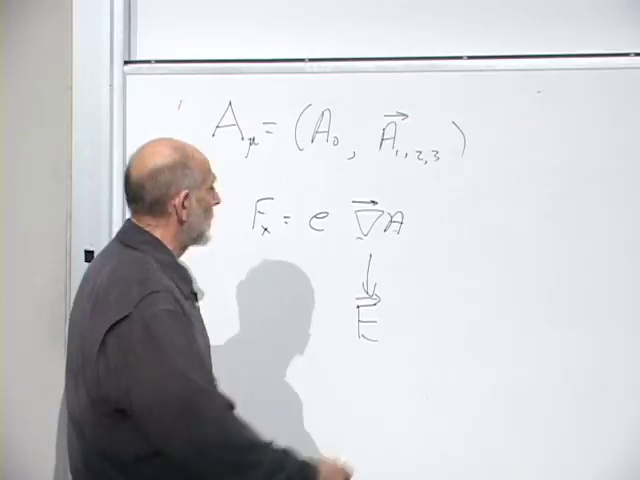
\includegraphics[width=0.62\textwidth]{lecture_05_figure_02.png}
\caption{電磁四維位勢及其與場之間的導數關係。}
\lectureframe{00:03:33}
\end{figure}

因此，電動力學有兩種等價的描述方式：一種以\(\boldsymbol E\)和\(\boldsymbol B\)描述，另一種則以\(A_\mu\)描述。後者只列出四個分量，因為不同的位勢可以描述相同的物理場。這種冗餘是「規範」一詞背後的第一個線索，不過我們暫時還不會正式使用這個概念。

\subsection{波與偏振}

麥克斯韋方程允許波動解。考慮一個沿單位向量\(\hat{\boldsymbol k}\)傳播的平面波。電場和磁場在每一點都與傳播方向垂直：
\begin{equation}
\boldsymbol E\cdot\hat{\boldsymbol k}=0,
\qquad
\boldsymbol B\cdot\hat{\boldsymbol k}=0,
\qquad
\boldsymbol E\cdot\boldsymbol B=0.
\end{equation}
在\(c=1\)的單位制下，兩者的大小相等：
\begin{equation}
|\boldsymbol E|=|\boldsymbol B|.
\end{equation}
對線偏振波而言，\(\boldsymbol E\)的方向決定偏振方向。整個波的形態以光速傳播。

量子化改變了描述方式，卻不改變偏振的結構。電磁波的量子就是光子。把光子畫成一個點難免會造成誤解，但不妨想像這個點帶著一根小小的橫向指針，標示其偏振方向。四分之一波片或其他光學元件可以旋轉偏振方向。靜態庫侖場也可以粗略地想像成由光子反覆發射與吸收所形成。

\subsection{源、通量與守恆}

電磁波可以在真空中傳播，但電磁場也有源：電荷與電流。正點電荷會產生向外的徑向電場，其大小正比於\(1/r^2\)。穿過以該電荷為中心的任意球面的場線數目，不隨球面半徑改變。以數學表示為
\begin{equation}
\oint_{S^2}\boldsymbol E\cdot d\boldsymbol S
=\frac{Q_{\mathrm{enc}}}{\epsilon_0},
\label{eq:l5-gauss}
\end{equation}
其中採用 SI 單位制。

這不只是計算電場的一種方便方法。電場線只能終止於電荷。若一個孤立電荷憑空消失，它的電場就必須同時在所有地方消失，這會違反因果律；或者，缺失電場的前沿必須向外傳播，讓場線終止於空無一物之處。這兩種情況都不允許。因此，通量的幾何性質自然導向電荷守恆：電荷可以移動，正負電荷可以湮滅，但若沒有相應電流補償，淨電荷就不能在局部消失。

相應的局域表述是連續方程：
\begin{equation}
\partial_t\rho+\boldsymbol\nabla\cdot\boldsymbol J=0.
\label{eq:l5-continuity}
\end{equation}
\editorialnote{方程~\eqref{eq:l5-continuity}是課堂上以口頭方式說明的因果性通量論證，所對應的標準局域數學形式。}

\subsection{規範理論的實用定義}

現在可以列出規範理論的基本模式。規範理論具有：
\begin{itemize}
\item 類似電場與磁場的場；
\item 在相互作用夠弱時，表現類似光波的波；
\item 類似電荷的源；
\item 將通量與這些源聯繫起來的高斯定律；
\item 守恆定律及其相關對稱性；
\item 稱為規範玻色子的場量子；以及
\item 控制玻色子發射與吸收的耦合常數。
\end{itemize}
源不一定是電荷。作為一個刻意選取的非物理例子，試想將重子數規範化。質子和中子的重子數都是\(+1\)，因此它們會透過一種新的類庫侖力互相排斥；質子與反質子則會互相吸引。這種理論在數學上可以想像，但自然界中並未觀測到與重子數耦合的長程規範場。單有守恆定律，並不保證存在規範力。

電荷確實伴隨著一種對稱性。對帶電物質場而言，
\begin{equation}
\psi(x)\longmapsto e^{i\theta}\psi(x).
\label{eq:l5-u1}
\end{equation}
相位對稱性與電荷守恆，是同一結構的兩個面向。稍後可以讓\(\theta\)依賴時空位置，藉此看出為什麼需要位勢\(A_\mu\)。在此處，全域變換已足以辨認守恆電荷。

\section{作為非阿貝爾例子的 QCD}

\subsection{三重態、反三重態與膠子矩陣}

在量子色動力學中，夸克場帶有色指標\(i\in\{r,g,b\}\)，並依照\(SU(3)\)的基本表示進行變換：
\begin{equation}
q'_i=U_{ij}q_j,
\qquad
U^\dagger U=\boldsymbol 1,
\qquad
\det U=1.
\label{eq:l5-q-transform}
\end{equation}
這是在三維複數色空間中的旋轉，而不是普通位置空間中的旋轉。這個三分量表示也稱為定義表示。

反粒子場以複共軛變數表示。對式~\eqref{eq:l5-q-transform}取複共軛，可得
\begin{equation}
q_i^{\prime *}=U_{ij}^*q_j^*.
\label{eq:l5-antiquark-transform}
\end{equation}
因此，夸克依照\(\boldsymbol 3\)變換，反夸克則依照\(\bar{\boldsymbol 3}\)變換。

\begin{figure}[htbp]
\centering
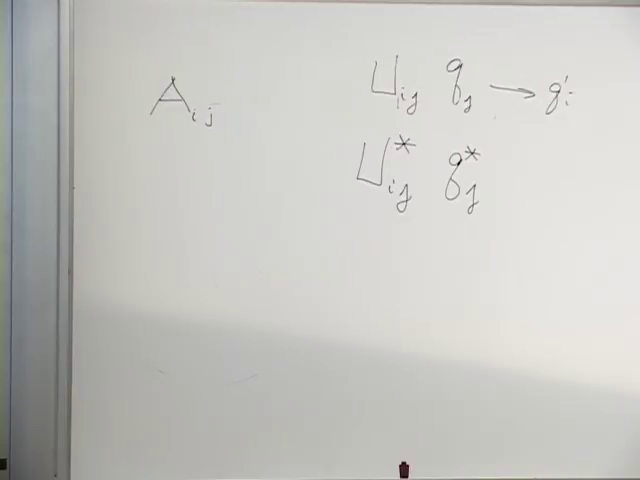
\includegraphics[width=0.62\textwidth]{lecture_05_figure_03.png}
\caption{基本表示的變換及其複共軛的反三重態變換。}
\lectureframe{00:18:47}
\end{figure}

\begin{classroomqa}
\audiencequestion{\(U\)矩陣有幾個？--七個、八個，還是九個？
\lecturetimestamp{00:19:37}}
\lecturerresponse{群元素\(U\)有無限多個。這裡要數的有限數目是獨立生成元的個數；對\(SU(3)\)而言，這個數目是八。一個一般的\(3\times3\)矩陣有九個矩陣元素位置，但特殊么正條件使其只有八個連續自由度。}
\end{classroomqa}

膠子場可以寫成無跡矩陣\(A_{ij}\)。其中一個指標像夸克那樣變換，另一個則像反夸克那樣變換，因此其色結構屬於
\begin{equation}
\boldsymbol 3\otimes\bar{\boldsymbol 3}
=\boldsymbol 1\oplus\boldsymbol 8.
\end{equation}
QCD 保留無跡的八重態：
\begin{equation}
A_{ii}=\operatorname{tr}A=0,
\end{equation}
並排除單態。這就是 QCD 有八種膠子而非九種的原因。更一般而言，\(SU(N)\)有
\begin{equation}
N^2-1
\end{equation}
個生成元，也有同樣數目的規範玻色子場。

光子在電荷\(U(1)\)作用下是中性的：旋轉電子的相位，不會把光子變換成另一種光子。膠子則不同。膠子帶有一個色和一個反色，因此屬於伴隨表示。例如，紅--反藍的組合並非色單態，儘管其中有一個色和一個反色。

\subsection{指標流與自相互作用}

追蹤指標就能讀出相互作用規則。概略而言，色為\(i\)的夸克可以變成色為\(j\)的夸克，同時發射一個帶有相應色流的膠子：
\begin{equation}
q_i\longrightarrow q_j+A_{ij}.
\label{eq:l5-quark-gluon-vertex}
\end{equation}
\(i\)和\(j\)的確切位置取決於箭頭的約定；不變的內容是，進入頂點的每個指標都必須沿著另一條線延續。沒有色指標會消失。

這項規則適用於任何\(SU(N)\)規範理論。基本表示的物質帶有一個指標，反基本表示的物質帶有一個共軛指標，而規範玻色子兩種指標各有一個。物理名稱可以不同，但指標結構不變。

膠子本身帶有色，因此可以發射另一個膠子。一個\(A_{ij}\)膠子可以經由中間指標\(k\)分裂，概略表示為
\begin{equation}
A_{ij}\longrightarrow A_{ik}+A_{kj}.
\label{eq:l5-three-gluon-index}
\end{equation}
這並非完整的楊--米爾斯頂點，但顯示了色流。在普通電動力學中，光子沒有類似的過程。因此膠子會對膠子施力，非阿貝爾場的動力學也比麥克斯韋線性理論複雜得多。

禁閉是其中一項定性的後果。色通量線不能終止，而其自相互作用會將它們拉成連接夸克與反夸克的管狀結構。管中的能量每單位長度大致固定：
\begin{equation}
V(R)\simeq \sigma R.
\end{equation}
因此，把兩端拉得更遠會儲存更多能量，而不是釋放出孤立的色荷。這就是膠子「黏稠」圖像中的關鍵：場本身會阻止帶色的組分以自由粒子形式逃逸。

\section{耦合常數與強弱的意義}

\subsection{電荷作為發射振幅}

規範理論還需要耦合常數。在 QED 中，電子電荷\(e\)是電子--光子頂點的相關係數。它是振幅，而機率是振幅的平方。從操作上來看，可以想像用陰極射線管讓一個高速電子突然停止。電子輻射出光子的機率正比於\(e^2\)；慣例上的因子則併入精細結構常數：
\begin{equation}
\alpha=\frac{e^2}{4\pi\hbar c}
\simeq \frac{1}{137}.
\label{eq:l5-alpha}
\end{equation}
在自然單位制\(\hbar=c=1\)下，耦合是無因次的。若單次基本發射的機率尺度約為百分之一，電磁相互作用在微擾意義下就算弱：大多數被迫停止的電子不會各自放出一簇高能光子。

\subsection{自然單位制連結能量、時間與距離}

令
\begin{equation}
c=1,
\qquad
\hbar=1.
\end{equation}
則時間與距離的單位相同，而能量的單位則是其倒數：
\begin{equation}
E=\hbar\omega\longrightarrow E=\omega\sim\frac1t,
\qquad
x\sim t\sim\frac1E.
\end{equation}
能量越高，所能探測的距離和時間尺度越短。

作為參照，
\begin{equation}
1\ {\rm eV}^{-1}
=\frac{\hbar c}{1\ {\rm eV}}
\simeq 1.97\times10^{-7}\ {\rm m}.
\end{equation}
因此，尺度約為\(10^{-10}\ {\rm m}\)的原子長度，大致相當於千電子伏特的倒數。這些只是數量級換算，並非精密光譜學的結果。

\subsection{原子內部的尺度層級}

以典型原子為例，取
\begin{equation}
R_{\rm atom}\sim10^{-10}\ {\rm m}.
\end{equation}
光穿越這段距離所需的時間為
\begin{equation}
t_{\rm transit}^{\rm atom}\sim10^{-18}\ {\rm s}.
\end{equation}
然而，在輕原子中，電子的速度只有光速的一小部分。依玻爾圖像，\(v/c\sim\alpha\)，因此典型的軌道週期更長：
\begin{equation}
t_{\rm orbit}^{\rm atom}\sim10^{-16}\ {\rm s}.
\end{equation}

激發態原子輻射衰變所需的時間還要更長：
\begin{equation}
t_{\rm decay}^{\rm atom}\sim10^{-9}\ {\rm s}
\end{equation}
這是課堂所用的大略估計。從物理圖像來看，有兩種抑制因素：電磁力所產生的加速度不大，而受加速的電子發射光子的機率也受到\(\alpha\)控制，並且很小。因此，精細結構常數小，使穿越時間、軌道時間與輻射衰變時間之間形成層級差異。

\subsection{強子中沒有這種層級差異}

強子是由夸克和膠子組成、類似原子的束縛系統，但其尺度小得多：
\begin{equation}
R_{\rm hadron}\sim10^{-15}\ {\rm m},
\qquad
t_{\rm transit}^{\rm hadron}\sim10^{-23}\ {\rm s}.
\end{equation}
夸克穿越強子的時間尺度幾乎相同，而會經由強作用衰變的激發態強子，其壽命也大約是
\begin{equation}
t_{\rm orbit}^{\rm hadron}
\sim t_{\rm decay}^{\rm hadron}
\sim10^{-23}\ {\rm s}.
\end{equation}
受撞擊的強子可能會振動並發射一個 {\proseunicodefont π} 介子，所需時間幾乎短到因果律所允許的極限。這裡不像原子內部那樣，存在相差七到九個數量級的時間尺度。

\begin{classroomqa}
\audiencequestion{狹義相對論是否表示，強子的衰變時間不可能顯著短於其光穿越時間？
\lecturetimestamp{00:47:15}}
\lecturerresponse{以數量級來說，這確實是合理的上限描述。強衰變發生得幾乎和系統尺度所允許的一樣快；沒有小耦合或其他大幅抑制因素拖慢它們。}
\end{classroomqa}

因此，相應的強耦合遠大於\(\alpha\)。在一個具代表性的強子尺度上，課堂引用的數值為
\begin{equation}
\alpha_{\rm QCD}\sim0.2,
\end{equation}
比起\(1/137\)更接近 1。這就是較早使用「\emph{強相互作用}」這個名稱的動力學根源。
\editorialnote{QCD 耦合會隨能量尺度而變，因此\(\alpha_s\)並非固定數值。這裡引用的是一個隨尺度而變的示例數值，符合課堂原意。}

\begin{classroomqa}
\audiencequestion{強作用的對應耦合是否就稱為強力常數？
\lecturetimestamp{00:48:17}}
\lecturerresponse{慣例上稱為\(\alpha_{\rm QCD}\)，更常稱為\(\alpha_s\)。電磁耦合通常簡稱\(\alpha\)；若在同一段討論中需要區分兩者，也可以用\(\alpha_{\rm QED}\)。}
\end{classroomqa}

\begin{classroomqa}
\audiencequestion{論文會區分裸電磁耦合與經測量、受到屏蔽的值嗎？
\lecturetimestamp{00:48:38}}
\lecturerresponse{會。通常會區分裸耦合與重整化耦合。真空極化會使有效耦合依測量尺度而變。}
\end{classroomqa}

\section{弱衰變之謎}

弱相互作用因衰變時間極長而得名。弱衰變通常比強衰變慢，有時甚至比原子輻射還慢。最早受到研究的例子是核 {\proseunicodefont β} 衰變。

\subsection{中子 {\proseunicodefont β} 衰變}

自由中子經由下列過程衰變：
\begin{equation}
n\longrightarrow p+e^-+\bar\nu_e.
\label{eq:l5-neutron-decay-intro}
\end{equation}
課堂採用的壽命約為 12 分鐘，和\(10^{-23}\ {\rm s}\)相比長得驚人。這裡的論證不需要用到現代的精密數值。

衰變緩慢的部分原因是運動學限制。大致而言，
\begin{equation}
\begin{aligned}
m_n&\simeq940\ {\rm MeV},
&
m_p&\simeq939\ {\rm MeV},
\\
m_e&\simeq0.5\ {\rm MeV}.
\end{aligned}
\end{equation}
中子的靜止能量只有極小一部分可轉為動能。若中子質量小於末態粒子的靜止質量總和，衰變便不可能發生；若中子質量只比閾值高出極微小的量，可用相空間就會極小，衰變也會很慢。但光靠相空間不足以解釋以分鐘計的壽命。

\subsection{帶電 {\proseunicodefont π} 介子排除了閾值這項解釋}

再考慮
\begin{equation}
\pi^-\longrightarrow e^-+\bar\nu_e
\end{equation}
以及其電荷共軛過程。{\proseunicodefont π} 介子的能量遠高於電子通道的閾值，但其弱衰變壽命仍在奈秒量級，而非強子過程的\(10^{-23}\)秒量級。稍後會談到一個類似的 {\proseunicodefont μ} 子通道。因此，這個謎題源自弱相互作用本身，而不只是中子質量近乎簡併所造成的偶然結果。

\editorialnote{帶電 {\proseunicodefont π} 介子的壽命約為\(26\ {\rm ns}\)，主要衰變通道是\(\pi^-\to\mu^-\bar\nu_\mu\)。電子通道受到螺旋度抑制。課堂先討論電子通道，因為其中粒子的記帳最簡單，接著再回頭討論主要的 {\proseunicodefont μ} 子通道。}

{\proseunicodefont β} 衰變一詞源自歷史上的用法：當時將衰變放出的電子稱為 {\proseunicodefont β} 射線。{\proseunicodefont π} 介子與中子的例子涉及相同的帶電流相互作用，儘管兩者的運動學條件差異很大。

\section{夸克與輕子表}

\subsection{色作用沿垂直方向}

將六種夸克味排列成三組配對的欄：
\begin{equation}
(u,d),\qquad(c,s),\qquad(t,b),
\end{equation}
再把每種夸克的紅、綠、藍三種色分別排在不同列。色作用\(SU(3)\)沿垂直方向進行：它會在上夸克的紅、綠、藍版本之間作變換，也會同時對下、粲、奇異、頂和底夸克進行相同的色變換。它不會把上夸克變成下夸克。

\subsection{弱同位旋作用沿水平方向}

弱對稱性則沿另一個方向作用，會混合下列每一對相鄰粒子：
\begin{equation}
Q_1=\begin{pmatrix}u\\d\end{pmatrix},
\qquad
Q_2=\begin{pmatrix}c\\s\end{pmatrix},
\qquad
Q_3=\begin{pmatrix}t\\b\end{pmatrix}.
\label{eq:l5-quark-doublets}
\end{equation}
上型夸克的電荷為\(+2/3\)，下型夸克的電荷為\(-1/3\)，所以每一對中的電荷相差一個單位。
\editorialnote{講者一度說下夸克的電荷是\(-2/3\)。根據前後的相減關係及後續各個過程，這裡採用標準值\(-1/3\)。}

由於這項對稱性作用於二重態，自然選用的群是\(SU(2)\)。它作用於每個夸克二重態的每一種色態，而不改變色。

還有一列粒子不帶色，因此不與膠子相互作用：輕子。它們另外組成三個二重態：
\begin{equation}
L_e=\begin{pmatrix}\nu_e\\e^-\end{pmatrix},
\qquad
L_\mu=\begin{pmatrix}\nu_\mu\\\mu^-\end{pmatrix},
\qquad
L_\tau=\begin{pmatrix}\nu_\tau\\\tau^-\end{pmatrix}.
\label{eq:l5-lepton-doublets}
\end{equation}
中微子不帶電；電子、{\proseunicodefont μ} 子和 {\proseunicodefont τ} 子的電荷則為\(-1\)。同樣地，每個二重態中的兩個成員電荷相差一個單位。電子、{\proseunicodefont μ} 子和 {\proseunicodefont τ} 子具有相同的規範量子數，但質量各不相同；三代上型夸克或下型夸克也有相同的電荷模式。

\begin{figure}[htbp]
\centering
\includegraphics[width=0.82\textwidth]{lecture_05_figure_05.png}
\caption{黑板上的表格：色作用連結紅、藍、綠各列；弱\(SU(2)\)則連結成對的味道欄，以及輕子列。}
\lectureframe{01:03:35}
\end{figure}

在此處把輕子稱為第四種色，只是一種類比。它們在弱同位旋二重態表中佔據第四列，但普通的 QCD \(SU(3)\)不會把夸克變換成輕子。

\section{建構帶電弱玻色子}

\subsection{帶電玻色子的量子數}

規範玻色子具有所需的變換性質，能將二重態的一個成員轉變為另一個。先看輕子對\(e^-\bar\nu_e\)。其電荷為\(-1\)，因此相應的帶電規範玻色子稱為\(W^-\)：
\begin{equation}
W^-\sim e^-\bar\nu_e.
\end{equation}
下夸克與反上夸克也有相同的量子數：
\begin{equation}
W^-\sim d\bar u.
\end{equation}
符號\(\sim\)表示兩者具有相同的相關規範量子數，並不表示\(W\)字面上是由這些粒子束縛而成。其反粒子由共軛組合構成：
\begin{equation}
W^+\sim e^+\nu_e\sim\bar d u.
\end{equation}

帶電弱頂點包括
\begin{align}
e^-&\longrightarrow\nu_e+W^-,
&
\mu^-&\longrightarrow\nu_\mu+W^-,
\label{eq:l5-lepton-w}\\
d&\longrightarrow u+W^-,
&
s&\longrightarrow c+W^-,
\label{eq:l5-quark-w}
\end{align}
運動學條件允許時，第三代粒子也有類似的躍遷。規範玻色子在動力學上實現了與對稱性作用於二重態時相同的水平混合。

\begin{classroomqa}
\audiencequestion{電荷守恆要求放出的玻色子電荷為\(-1\)，但為什麼電子、下夸克和奇異夸克的躍遷都涉及同一種粒子？
\lecturetimestamp{01:12:56}}
\lecturerresponse{這是由共同的弱對稱性所反映的一項實驗事實。自然界完全可以自洽地為每個世代，或分別為夸克與輕子，指定不同的\(W\)型玻色子。但實際上，一個\(SU(2)\)同時作用於所有二重態，而所有這些躍遷都由相同的帶電規範玻色子媒介。}
\end{classroomqa}

\subsection{讀取與反轉頂點}

一個頂點代表一系列過程。將入射線反轉為出射線，會使粒子變成其反粒子；將\(W^-\)線反轉，則會得到\(W^+\)。因此，只要一致地追蹤電荷、動量及所有相關量子數，同一頂點可以描述發射、吸收、衰變、湮滅或其逆反應。

\begin{classroomqa}
\audiencequestion{這些弱頂點中的箭頭和線可以反向嗎？
\lecturetimestamp{01:14:51}}
\lecturerresponse{可以。線可以由末態交叉至初態，或由初態交叉至末態；但如此一來，粒子就會變成其反粒子。因此，同一個局域頂點可以描述許多方向不同的反應。}
\end{classroomqa}

\begin{classroomqa}
\audiencequestion{把奇異夸克線和粲夸克線畫進\(W^-\)，是否表示這個玻色子字面上是由奇異夸克和反粲夸克束縛而成？
\lecturetimestamp{01:15:43}}
\lecturerresponse{不是。線的記帳只表示\(W^-\)承載了這些欄位之間的量子數變化。若把圖讀作衰變，能量足夠高的\(W^-\)可以產生一個奇異夸克和一個反粲夸克；它本身並不是由這兩者組成。}
\end{classroomqa}

\begin{classroomqa}
\audiencequestion{電子和反中微子能否形成\(W\)，再由它產生一對夸克？
\lecturetimestamp{01:17:22}}
\lecturerresponse{正是如此。只要質心能量足夠，初態輕子便能形成帶電流中間態，而這個中間態可以透過允許的夸克通道出現。這兩個頂點和衰變過程中的頂點相同，只是從另一個方向來讀。}
\end{classroomqa}

\subsection{缺少的第三種玻色子}

\(SU(2)\)群有三個生成元，因此有三個規範場。目前只列出了\(W^+\)和\(W^-\)。第三個電中性場必須對應於一些對角組合，例如電子--正電子以及中微子--反中微子的量子數組合。這個場刻意暫置於背景中。它與物理的\(Z\)玻色子及光子的關係，則要等到討論電弱混合時才會說明。

\begin{classroomqa}
\audiencequestion{弱作用和強作用是在不同的歷史時期才受到懷疑的嗎？
\lecturetimestamp{01:24:11}}
\lecturerresponse{兩者的實驗起源都可追溯至早期放射性研究。{\proseunicodefont α} 衰變揭示了核物理與強相互作用，{\proseunicodefont β} 衰變揭示了弱相互作用，而 {\proseunicodefont γ} 衰變則放出電磁光子。早在貝克勒爾的年代，這三項線索就已經全數出現，遠早於現代場論的建立。}
\end{classroomqa}

\section{帶電流衰變範例}

\subsection{{\proseunicodefont π} 介子衰變}

帶負電 {\proseunicodefont π} 介子的價夸克組成為
\begin{equation}
\pi^-=d\bar u.
\end{equation}
這些量子數可以透過湮滅形成\(W^-\)，再由它產生一個帶電輕子及相應的反中微子：
\begin{align}
\pi^-&\longrightarrow W^{-*}
\longrightarrow e^-+\bar\nu_e,
\label{eq:l5-pion-electron}\\
\pi^-&\longrightarrow W^{-*}
\longrightarrow \mu^-+\bar\nu_\mu.
\label{eq:l5-pion-muon}
\end{align}
星號表示中間的\(W\)是虛粒子。第二個通道是主要衰變通道。

\begin{figure}[htbp]
\centering
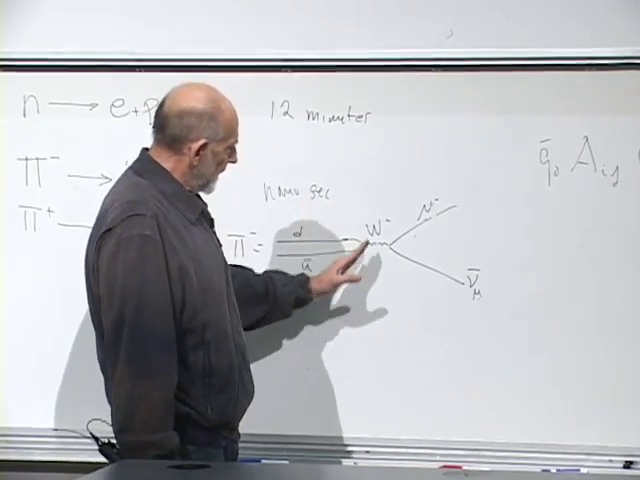
\includegraphics[width=0.72\textwidth]{lecture_05_figure_04.png}
\caption{一個\(d\bar u\){\proseunicodefont π} 介子湮滅形成虛\(W^-\)，接著產生一個帶電輕子及其相應的反中微子。}
\lectureframe{01:19:38}
\end{figure}

\begin{classroomqa}
\audiencequestion{時間方向畫成水平而非垂直，這樣仍算是費曼圖嗎？
\lecturetimestamp{01:20:21}}
\lecturerresponse{算。時間軸在紙面上的方向只是一種約定。只要先指定一個方向代表時間，並一致地解讀所有箭頭，這張圖所表達的相互作用資訊就相同。}
\end{classroomqa}

\begin{classroomqa}
\audiencequestion{這張圖能不能像可逆化學反應那樣來解讀，而不是看成單向、不可逆的衰變？
\lecturetimestamp{01:21:35}}
\lecturerresponse{逆過程是允許的。在真空中產生的 {\proseunicodefont π} 介子會衰變，是因為出射粒子彼此分離，通常不會重新結合。但若讓 {\proseunicodefont μ} 子和反中微子以適當的能量與動量一同撞入，經由反向相互作用形成 {\proseunicodefont π} 介子的振幅便不為零。}
\end{classroomqa}

\subsection{能量與虛中間態}

對於靜止的 {\proseunicodefont π} 介子，
\begin{equation}
m_\pi\simeq140\ {\rm MeV},
\qquad
m_\mu\simeq106\ {\rm MeV},
\qquad
m_\nu\approx0
\end{equation}
在此處所需的精度下，這些數值近似成立。剩餘能量會轉為出射粒子的動能。動量守恆要求
\begin{equation}
\boldsymbol p_\mu+\boldsymbol p_{\bar\nu}=0,
\end{equation}
因此，兩個粒子在 {\proseunicodefont π} 介子的靜止參考系中背向飛離。

\begin{classroomqa}
\audiencequestion{中間態\(W\)的質量遠大於 {\proseunicodefont π} 介子，能量怎麼可能守恆？
\lecturetimestamp{01:25:08}}
\lecturerresponse{只有初態和末態粒子必須位於質量殼上。四動量在每個頂點都守恆，但內部虛線不必滿足\(E^2=\boldsymbol p^2+m_W^2\)。離殼偏差越大，其傳播子對過程的抑制就越強。\editorialnote{講座使用了傳統的能量--時間不確定性說法，並表示中間態可以短暫違反能量守恆。更精確的現代表述如回答所述：能量—動量守恆，但內部虛線不必滿足實粒子的質量殼條件。}}
\end{classroomqa}

\subsection{{\proseunicodefont μ} 子衰變}

{\proseunicodefont μ} 子可以先放出一個虛\(W^-\)，轉變成其對應的中微子：
\begin{equation}
\mu^-\longrightarrow\nu_\mu+W^{-*}.
\end{equation}
接著，這個虛玻色子會產生一個電子和一個電子反中微子：
\begin{equation}
\mu^-\longrightarrow
\nu_\mu+e^-+\bar\nu_e.
\label{eq:l5-muon-decay}
\end{equation}
這是純輕子過程。{\proseunicodefont μ} 子的質量約為電子的 200 倍，因此末態粒子的靜止質量之外，還有充足能量可轉化為動能。

\begin{figure}[htbp]
\centering
\includegraphics[width=0.72\textwidth]{lecture_05_figure_06.png}
\caption{{\proseunicodefont μ} 子經由虛帶電弱玻色子衰變。}
\lectureframe{01:29:24}
\end{figure}

\begin{classroomqa}
\audiencequestion{與電子一同發射的中性粒子是反中微子嗎？
\lecturetimestamp{01:29:06}}
\lecturerresponse{是的。完整的末態包含一個 {\proseunicodefont μ} 中微子、一個電子反中微子和一個電子。保留味標籤，就能避免混淆這兩個中性粒子。}
\end{classroomqa}

電子在真空中無法逆向進行這個衰變，因為電子比 {\proseunicodefont μ} 子輕。{\proseunicodefont τ} 子較重，可以經由類似的弱作用通道衰變。這裡的穩定性部分只是質量排序所造成的偶然結果，並非底層頂點有所不同。

\begin{classroomqa}
\audiencequestion{直線加速器是否等於有效地增加電子的質量，讓原本禁戒的反應得以反向進行？
\lecturetimestamp{01:30:23}}
\lecturerresponse{它不會改變電子的不變靜止質量，而是提供動能。足夠的質心能量可以產生較重的末態粒子；因此，只要將質量改成可用的碰撞能量，這個物理想法就是正確的。}
\end{classroomqa}

\subsection{夸克層次的中子 {\proseunicodefont β} 衰變}

中子和質子的價夸克組成如下：
\begin{equation}
n=udd,
\qquad
p=uud.
\end{equation}
中子中的一個下夸克經歷帶電流躍遷：
\begin{equation}
d\longrightarrow u+W^{-*},
\end{equation}
使 \(udd\) 轉變為 \(uud\)。接著，虛玻色子衰變為：
\begin{equation}
W^{-*}\longrightarrow e^-+\bar\nu_e.
\end{equation}
將這兩個頂點結合起來，就會得到
\begin{equation}
n\longrightarrow p+e^-+\bar\nu_e.
\end{equation}

相反的夸克躍遷 \(u\to d+W^+\) 會留下由三個下夸克組成的重子，但這個可達到的末態對自由中子而言太重，無法產生。實際發生的下夸克轉變為上夸克，才是能量上允許的路徑。

\begin{classroomqa}
\audiencequestion{中子能不能改為衰變成一個質子、一個 {\proseunicodefont μ} 子和相應的反中微子？
\lecturetimestamp{01:32:38}}
\lecturerresponse{對於靜止的自由中子而言，不能：中子--質子的質量差遠小於 {\proseunicodefont μ} 子的質量。若有足夠的額外碰撞能量或激發能量，同一個弱作用頂點也能參與產生 {\proseunicodefont μ} 子的反應通道。這是運動學上的禁戒，並非缺少相互作用。}
\end{classroomqa}

\section{尚未解開的壓低之謎}

帶電弱作用頂點說明了哪些過程可以發生，卻還沒有解釋它們為何如此緩慢。一個看似合理的答案是弱耦合極其微小，但這個答案不對：無因次的弱規範耦合大小大致與電磁耦合相當。這種壓低必定另有原因。

虛傳播子已顯示出缺少的關鍵：\(W\)的質量非常大。在遠低於 \(m_W\) 的能量下，帶電流振幅會受到大致與 \(1/m_W^2\) 的冪次成比例的壓低。待希格斯機制和電弱對稱性破缺說明規範玻色子如何獲得質量後，我們再來展開這個關聯。
\editorialnote{講座將這個問題留待下一次課程討論。此處納入重 \(W\) 的解釋，是為了預先連結後續內容，並非表示這項推導已在本講座中完成。}

\begin{classroomqa}
\audiencequestion{我們說這個理論具有這種對稱性，是指它的拉格朗日量在相應的變換下保持不變嗎？
\lecturetimestamp{01:34:14}}
\lecturerresponse{正是如此。說這個理論具有該對稱性，是指拉格朗日量，或等價地說，作用量在這些變換下保持不變。完整的拉格朗日量只是留待之後寫出，並非改用其他定義。}
\end{classroomqa}

這條脈絡至此已完整：麥克斯威理論提供原型；QCD 展示非阿貝爾規範玻色子如何攜帶並交換荷；耦合常數說明原子與強子的時間尺度為何不同；而弱 \(SU(2)\) 則將夸克和輕子組成由 \(W^\pm\) 相連的二重態。接下來要理解的是，為什麼這些由規範作用中介的過程在實際上如此微弱，儘管其底層耦合並不特別小。
\chapter{有質量弱交換、虛粒子與對稱性破缺}

把標準模型群看成費米子表上允許的各種變換，許多疑問便不再那麼神秘。色變換在紅、綠、藍之間作垂直變換；帶電弱變換則在夸克與輕子的二重態內作水平變換。電磁相位變換提供第三種操作。相應的規範玻色子並非發現對稱性後才添上的裝飾：發射規範玻色子，在物理上實現的正是對稱性生成元所描述的狀態變換。

這個觀察引出本講的主要問題。弱作用頂點的耦合與電磁作用頂點的耦合大小相近，但{\proseunicodefont β}衰變卻比典型的強作用或電磁過程慢得多。關鍵在於傳播。在低動量下，交換有質量的\(W\)會使振幅乘上一個量級為\(1/m_W^2\)的因子。我們會先在距離空間、再在動量空間推導這個說法，接著透過一段關於實粒子與虛粒子的長篇討論追溯其後果，最後轉向自發對稱性破缺的第一個定性模型。

\section{從費米子表看規範對稱性}

\subsection{色變換沿垂直方向進行}

將六種夸克味排列成三個弱作用家族，
\begin{equation}
  (u,d),\qquad(c,s),\qquad(t,b),
\end{equation}
再為每個夸克標上紅、綠或藍色。如此得到的夸克表有三列顏色、六欄味。色\(SU(3)\)會混合任一味欄中的三個夸克。例如，一個生成元可以將紅色上夸克變換為綠色上夸克。用粒子語言來說，同一個變換會伴隨一個帶有補償色荷與反色荷的膠子發射。

同一個色變換必須作用於所有味。將紅色上夸克變換為綠色上夸克的膠子，與將紅色頂夸克變換為綠色頂夸克的膠子，屬於同一種粒子。一個真正的對稱變換不會只作用於第一代而忽略其他代。因此，色變換沿垂直方向進行，且普遍作用於所有味：
\begin{equation}
  q_r\longleftrightarrow q_g\longleftrightarrow q_b,
  \qquad q\in\{u,d,c,s,t,b\}.
\end{equation}
它改變顏色，不改變味。

這正是規範群與其規範玻色子之間的典型關係。無窮小生成元描述狀態之間的變換，而發射或吸收相應的玻色子，則會在物理過程中實現這些變換。

\subsection{弱變換沿水平方向進行}

帶電弱作用沿另一個方向進行。上型夸克可以發射帶電弱玻色子，轉變為它的下型夥伴，而不改變顏色：
\begin{equation}
  u_b\longrightarrow d_b+W^+.
\end{equation}
同樣的\(W^+\)也會出現在
\begin{equation}
  c_g\longrightarrow s_g+W^+,
  \qquad
  t_r\longrightarrow b_r+W^+.
\end{equation}
標記\(r,g,b\)不受影響。膠子不會沿表格水平方向變換，帶電的\(W\)玻色子也不會沿顏色方向垂直變換。

再加入電磁相位對稱性\(U(1)\)；在此變換下，每個帶電場都會取得一個相位。初步的群結構便是
\begin{equation}
  SU(3)\times SU(2)\times U(1).
\end{equation}
叉號表示這些是彼此獨立的因子：一個作用於顏色，一個作用於弱二重態，另一個則透過相位作用。這是有用的粗略圖像，但還不是完整的電弱理論。\editorialnote{標準模型的規範群通常精確寫成
\(SU(3)_c\times SU(2)_L\times U(1)_Y\)。弱作用的\(SU(2)_L\)只作用於左手二重態，而最終的電磁\(U(1)_{\rm em}\)則在對稱性破缺後由\(SU(2)_L\times U(1)_Y\)湧現。本講特別提醒，初步將最後兩個因子如此對應，仍不完全一致；後續各講會補上缺少的手徵結構與電弱結構。}

\subsection{輕子也遵循同樣的模式}

在三列夸克顏色下方，放上一列不帶色荷的輕子：
\begin{equation}
\begin{array}{c|cc|cc|cc}
 &u&d&c&s&t&b\\ \hline
Q&+\frac23&-\frac13&+\frac23&-\frac13&+\frac23&-\frac13\\
\text{lepton partner}
 &\nu_e&e^-&\nu_\mu&\mu^-&\nu_\tau&\tau^-\\
Q&0&-1&0&-1&0&-1
\end{array}
\end{equation}
每一對相鄰項目的電荷都相差一個單位。這就是同一個帶電弱玻色子能連接\(u\)與\(d\)、\(c\)與\(s\)、\(t\)與\(b\)，以及帶電輕子與其中微子的原因。\(W\)頂點取決於相應的量子數與電荷差，而不在於費米子是夸克還是輕子。

\begin{figure}[htbp]
\centering
\includegraphics[width=0.88\textwidth]{lecture_06_figure_07.png}
\caption{完整的費米子表：三列不同顏色的夸克位於不帶色荷的輕子列上方，可清楚看出夸克電荷與三個輕子二重態。}
\lectureframe{00:18:55}
\end{figure}

{\proseunicodefont μ}子的電荷與已知內禀量子數都和電子相同，但質量約為電子的兩百倍。{\proseunicodefont τ}子更重。中微子的質量非常小；在本講討論時，相關細節尚未明朗。到目前為止，還沒有任何原理能解釋觀察到的各家族質量模式。

\begin{classroomqa}
\audiencequestion{為什麼輕子、重子和介子會使用這些名稱？
\lecturetimestamp{00:19:02}}
\lecturerresponse{這些名稱的希臘語詞根，歷史上大致分別指輕、重和中間。這種依質量命名的方式後來顯得容易誤導。{\proseunicodefont μ}子曾稱為{\proseunicodefont μ}介子，因為它的質量介於電子與質子之間；但從相互作用來看，它屬於輕子，和電子遠比和{\proseunicodefont π}介子相似。現在，介子是指由夸克--反夸克組成的強子，且屬於玻色子；{\proseunicodefont μ}子不是介子。}
\end{classroomqa}

\section{弱作用為何如此弱？}

\subsection{一個具體的帶電流過程}

以中子{\proseunicodefont β}衰變作為例子。其價夸克組成為
\begin{equation}
  n=udd,\qquad p=uud.
\end{equation}
其中一個下夸克發生轉變：
\begin{equation}
  d\longrightarrow u+W^-,
\end{equation}
帶電玻色子則產生
\begin{equation}
  W^-\longrightarrow e^-+\bar\nu_e.
\end{equation}
合起來就是
\begin{equation}
  n\longrightarrow p+e^-+\bar\nu_e.
\end{equation}
另外兩個價夸克在過程中維持不變，作為旁觀者。第一個頂點上，中子轉變為質子；第二個頂點上，將輕子二重態連接起來的同一種弱作用，則把\(W^-\)轉變為觀察到的電子與電子反中微子。

\subsection{三種耦合，三種截然不同的印象}

在量子電動力學（QED）中，電子電荷\(e\)就是頂點振幅。將其平方可得典型的發射機率；採用自然單位制時，慣例因子都收在
\begin{equation}
  \alpha=\frac{e^2}{4\pi}\simeq\frac1{137}
\end{equation}
之中。強作用的耦合為\(g_s\)；在典型的強子尺度上，相應的量\(\alpha_s\)可能約為\(0.2\)。這遠大於\(1/137\)，所以夸克受到撞擊時，膠子很容易發射。

令\(g_w\)表示帶電弱作用的耦合。它的平方並沒有小得驚人；依這裡採用的數量級估算，它與電磁耦合相當。然而，自由中子平均要等待約十五分鐘才衰變；強衰變則可能在強子穿越自身尺度所需的時間內發生。本講的歷史估算採用較早的粗略數字十二分鐘，但無論採用哪個數字，同一個疑問都無可迴避。\editorialnote{現代測得的自由中子平均壽命約為\(8.8\times10^2\,{\rm s}\)，而主要測量方法之間至今仍存在實驗上的張力。本講保留的粗略壽命是教學用的尺度估計，並非精確值。}
\begin{quote}
如果\(g_w\)沒有小得異常，究竟是什麼讓弱過程顯得弱？
\end{quote}

答案不能只從頂點尋找。每張費曼圖也包含傳播子；這些因子描述從一個頂點到另一個頂點的中間傳播。

\section{距離空間中的有質量傳播子}

\subsection{頂點並非整張圖的全部}

{\proseunicodefont β}衰變圖包含兩個弱作用頂點，各貢獻一個\(g_w\)，以及一條連接兩個頂點的\(W\)線。將位置空間中的傳播子記為\(\Delta(x-y)\)，其中\(x\)是發射事件的位置，\(y\)是吸收或轉換事件的位置。這個振幅核描述場的擾動如何在兩個事件之間傳播。

精確的相對論性傳播子包含許多此處用不著的結構。重要的定性特徵是它對質量的依賴。在短的類空間隔下，它有冪律奇異性，示意如下：
\begin{equation}
  \Delta(d)\sim\frac1{d^2}.
\end{equation}
無質量場會保留冪律尾端；相較之下，當距離遠大於有質量場的康普頓尺度時，傳播會受到指數抑制。因此，曲線會急遽向下彎折。

\subsection{自然單位制指出彎折位置}

令
\begin{equation}
  c=\hbar=1.
\end{equation}
則
\begin{equation}
  [m]=[E]=[p]=L^{-1}.
\end{equation}
熟悉的關係說明了這些等式：\(E=mc^2\)把質量與能量聯繫起來；而\(p\,x\)的量綱是\(\hbar\)，因此動量與距離的單位互為倒數。由質量\(m\)能構成的唯一長度尺度因此是
\begin{equation}
  d_m\sim\frac1m.
\end{equation}
恢復常數後可得
\begin{equation}
  d_m\sim\frac{\hbar}{mc},
\end{equation}
也就是康普頓波長。交換粒子的質量越大，有效作用距離越短。

\begin{figure}[htbp]
\centering
\includegraphics[width=0.78\textwidth]{lecture_06_figure_02.png}
\caption{自然單位制下的量綱，以及傳播子定性衰減的示意圖。黑色曲線繼續呈現冪律尾端；紅色的有質量曲線則在反質量尺度附近開始急遽下降。}
\lectureframe{00:27:19}
\end{figure}

\begin{figure}[htbp]
\centering
\begin{tikzpicture}[x=1.0cm,y=0.9cm]
  \draw[->] (0,0) -- (7,0) node[right] {$d$};
  \draw[->] (0,0) -- (0,5) node[above] {$|\Delta(d)|$};
  \draw[thick]
    plot[smooth] coordinates {(0.45,4.5) (0.9,3.3) (1.6,2.5)
      (2.5,1.9) (3.7,1.45) (5.1,1.12) (6.4,0.9)};
  \draw[thick,red]
    plot[smooth] coordinates {(0.45,4.5) (0.9,3.3) (1.6,2.5)
      (2.5,1.9) (3.2,1.55) (3.7,0.95) (4.2,0.36) (4.8,0.1)};
  \draw[dashed] (3.4,0) -- (3.4,1.4);
  \node at (5.7,1.4) {$m=0$};
  \node[red] at (4.75,0.72) {$m>0$};
  \node[below] at (3.4,0) {$d\sim m^{-1}$};
\end{tikzpicture}
\caption{黑板論證的簡明示意圖。這不是四維傳播子的精確公式，而是用來呈現由質量控制的作用距離。}
\end{figure}

\begin{classroomqa}
\audiencequestion{縱軸表示什麼？
\lecturetimestamp{00:28:30}}
\lecturerresponse{縱軸表示傳播子的大小，記作\(\Delta\)。完整振幅、外部態和相空間因子都納入後，它的平方才會對機率有所貢獻。圖中要表達的是，經由有質量粒子交換的振幅在長距離下會迅速衰減。\editorialnote{傳播子本身並不是可直接測量、描述粒子沿經典路徑運動的機率振幅。本講用這種說法作為有用的作用距離估算：傳播子只是完整散射或衰變振幅中的一個因子。}}
\end{classroomqa}

\section{傅立葉變換與費米極限}

\subsection{實驗測量的是動量}

實驗通常測量外部粒子的動量，而不是內部線在何處開始、何處結束。在{\proseunicodefont β}衰變中，\(W\)所帶的動量可由中子與質子的動量差推得；這個動量也等於電子與反中微子的總動量。位置空間與動量空間中的傳播子，彼此透過傅立葉變換相連。
\begin{equation}
  k=p_n-p_p=p_e+p_{\bar\nu_e}.
\end{equation}

依照黑板上採用的正分母慣例，
\begin{equation}
  \widetilde{\Delta}_W(k)=\frac1{k^2+m_W^2},
  \qquad
  \widetilde{\Delta}_\gamma(k)=\frac1{k^2}.
\end{equation}
無質量光子的傳播子在動量轉移很小時會變得很大。有質量的\(W\)傳播子則不會超過\(1/m_W^2\)量級。對{\proseunicodefont β}衰變而言，
\begin{equation}
  |k^2|\ll m_W^2,
\end{equation}
因此，\(k^2\)的細節可以忽略，並且
\begin{equation}
  \widetilde{\Delta}_W(k)\simeq\frac1{m_W^2}.
\end{equation}

\begin{classroomqa}
\audiencequestion{相對論性記號中的\(k^2\)，在能量與空間動量之間是否應該有一個負號？
\lecturetimestamp{00:35:11}}
\lecturerresponse{是的。採用空間分量為負號的閔可夫斯基度規時，
\(k^2=(k^0)^2-\boldsymbol{k}^2\)；而純量分母通常寫成
\(k^2-m_W^2+i\epsilon\)。黑板上使用的是與此等價的正值空間類或歐幾里得大小。低能{\proseunicodefont β}衰變中的四動量轉移遠小於\(m_W\)，因此無論採用哪種記號，得到的\(1/m_W^2\)抑制都相同，振幅至多只差一個無關緊要的符號。}
\end{classroomqa}

\subsection{低能振幅}

兩個弱作用頂點與一個傳播子給出
\begin{align}
  \mathcal A_{\rm weak}
  &\sim g_w\,\widetilde{\Delta}_W(k)\,g_w\\
  &\sim\frac{g_w^2}{k^2+m_W^2}
  \simeq\frac{g_w^2}{m_W^2}.
\end{align}
將振幅平方後，便得到典型的抑制因子
\begin{equation}
  |\mathcal A_{\rm weak}|^2
  \sim\frac{g_w^4}{m_W^4},
\end{equation}
這還沒有納入特定衰變所對應的運動學與相空間因子。弱作用在核能標下之所以弱，不是因為它的基本規範耦合小得離譜，而是因為媒介粒子的質量很大。

\begin{figure}[htbp]
\centering
\includegraphics[width=0.86\textwidth]{lecture_06_figure_03.png}
\caption{中子--質子弱作用過程，以及內部線所傳遞的動量轉移；這正是確定傳播子符號時所討論的內容。}
\lectureframe{00:35:40}
\end{figure}

\begin{figure}[htbp]
\centering
\includegraphics[width=0.84\textwidth]{lecture_06_figure_04.png}
\caption{{\proseunicodefont β}衰變的圖形拓撲，旁邊列有方框中的低能估算\(g_w^2/m_W^2\)。}
\lectureframe{00:37:25}
\end{figure}

依照本講使用的精度，\(m_W\)約為質子質量的一百倍。振幅中的\(m_W^{-2}\)因子，在衰變率中會變成\(m_W^{-4}\)；因此，即使耦合大小與一般規範理論相當，也會造成極長的壽命。

\begin{classroomqa}
\audiencequestion{這裡說的抑制是百萬分之一，還是十億分之一？\(W\)的質量最初又是如何得知的？
\lecturetimestamp{00:38:11}}
\lecturerresponse{本講的粗略估算指出，低能弱作用的機率相對於未受抑制的強子過程，小了約十億倍。從歷史上來看，低能實驗並沒有分別測量\(g_w\)與\(m_W\)，而是測量一個較小的組合量：
\(g_w^2/m_W^2\)
這個量稱為費米常數。當規範耦合與電弱理論建立關聯後，這個組合量便預測媒介粒子的質量很大；後來，加速器直接產生\(W\)並測得其質量。}
\end{classroomqa}

當動量遠低於\(m_W\)時，所有實驗測得的結果都幾乎由同一個常數描述：
\begin{equation}
  G_F\sim\frac{g_w^2}{m_W^2}.
\end{equation}
這就是為什麼費米早在1930年代，就能把{\proseunicodefont β}衰變描述成點狀的四費米子交互作用，遠早於媒介粒子被觀測到。隨著碰撞能量提高，實驗開始能探測到隱藏在傳播子中的動量依賴，證實這個有效常數是有質量粒子交換在低能下留下的影子。\editorialnote{採用標準電弱理論的樹圖階歸一化時，
\[
  \frac{G_F}{\sqrt2}=\frac{g^2}{8m_W^2}.
\]
本講刻意省略數值因子與旋量因子，只保留標度關係\(G_F\sim g_w^2/m_W^2\)。\(W\)與\(Z\)於1983年在歐洲核子研究組織（CERN）首次直接發現；本講順帶提到的1970年代中後期，對於直接觀測而言還太早。}

從歷史上來看，弱作用可能由重粒子媒介的構想出現在二十世紀中葉。本講提到朱利安・施溫格是曾探討這種可能性的理論物理學家之一，也指出字母\(W\)很可能代表弱作用。早在加速器有足夠能量將這種媒介粒子實際產生出來之前，低能資料便已顯示，它在核能標下必須極其沉重。

\subsection{決定衰變率的三項獨立因素}

課堂上關於核束縛的一個問題，帶出影響躍遷的三項彼此獨立的因素：
\begin{enumerate}
  \item 頂點耦合常數；
  \item 傳播子，包括質量與動量依賴性；
  \item 初態與末態之間可用的能量，以及相空間。
\end{enumerate}
束縛可能使某個衰變道無法發生，因為末態能量會高於初態。這是運動學上的禁止，不是進一步降低\(g_w\)，也不是改變\(m_W\)。若衰變道仍然開放，但可用能量很少，相空間仍可能受到強烈抑制。

\begin{classroomqa}
\audiencequestion{附近質子的場或束縛，會不會透過相同的傳播子機制抑制{\proseunicodefont β}衰變？
\lecturetimestamp{00:41:13}}
\lecturerresponse{在這裡討論的例子中，不會。束縛會造成影響，是因為它改變了初態與末態核態的能量。若末態在能量上無法到達，過程就不能發生。耦合、傳播子與可用能量是三項彼此獨立的因素。}
\end{classroomqa}

\begin{classroomqa}
\audiencequestion{耦合常數真的不變嗎？
\lecturetimestamp{00:42:55}}
\lecturerresponse{只有在固定的能標下才能這麼說。量子修正會使有效耦合隨動量或距離改變，這稱為耦合的跑動。本段論證以該過程相關能標下的耦合為準；後續會進一步討論能標依賴性。}
\end{classroomqa}

\section{不違反守恆律的虛粒子交換}

\subsection{重粒子線為何能出現在圖中}

普通的中子衰變沒有足夠能量產生自由且在質殼上的\(W\)。圖中的\(W\)是內部線，且處於離殼狀態。本講以傳統的能量--時間估算引入這個概念：
\begin{equation}
  \Delta E\,\Delta t\lesssim\hbar:
\end{equation}
一個能量看似偏差\(\Delta E\)的中間組態，只能在約
\(\hbar/\Delta E\)的時間內有所貢獻。

隧穿的類比能讓這個圖像更清楚。設想一個{\proseunicodefont α}粒子處於核勢阱中。它的能量低於勢壘頂，因此按經典力學無法逃逸。量子力學中的波函數可以延伸穿過勢壘，粒子也能在勢壘另一側出現，且總能量與初始時相同。如果試圖以一般的經典軌跡描述勢壘內部，勢能似乎太高，因而必須有負的動能。這種失敗的經典圖像，類似於把內部的\(W\)當成實粒子。

\begin{figure}[htbp]
\centering
\includegraphics[width=0.78\textwidth]{lecture_06_figure_06.png}
\caption{隧穿類比：起始點與遠側斜坡上的標記點具有相同的總能量，中間的勢壘區則是經典力學所禁止的區域。}
\lectureframe{00:46:00}
\end{figure}

\begin{figure}[htbp]
\centering
\begin{tikzpicture}[x=1.0cm,y=0.9cm]
  \draw[->] (0,0) -- (7,0) node[right] {$x$};
  \draw[->] (0,0) -- (0,4.8) node[above] {$V(x)$};
  \draw[thick]
    plot[smooth] coordinates {(0.3,1.4) (1.0,0.7) (1.7,0.55)
      (2.1,0.9) (3.2,3.9) (4.2,2.1) (5.0,0.75) (6.6,0.18)};
  \draw[dashed] (1.7,0.75) -- (5.0,0.75);
  \fill (1.7,0.75) circle (0.06);
  \fill (5.0,0.75) circle (0.06);
  \node at (3.35,0.35) {$\Delta E\,\Delta t\lesssim\hbar$};
\end{tikzpicture}
\caption{勢壘與等能量點的清晰重繪示意。}
\end{figure}

在{\proseunicodefont β}衰變的圖像中，中子可能短暫漲落為質子與內部的\(W^-\)，但這條重粒子線必須很快消失。它可能被重新吸收，使中子恢復原狀；也可能在第二個頂點終止，產生輕得多的電子與反中微子。整體而言，初態與末態的能量相同。\editorialnote{每個費曼頂點都遵守能量與動量守恆。虛粒子並不是先借用能量、稍後再歸還。精確地說，內部線的四動量需要積分，而積分所涵蓋的四動量不一定滿足實粒子的質殼關係\(k^2=m_W^2\)。本講以不確定性原理和隧穿作為解說途徑，因此仍保留這些說法；不過，離殼才是現代量子場論中的精確表述。}

\subsection{實際產生的W玻色子}

能量足夠高的加速器可以產生實際的\(W\)。它有自己的固有壽命，與假想的虛粒子線所對應的不確定時間無關。依照一般的相對論時間膨脹，運動中的\(W\)在實驗室參考系中會存活較久。靜止的\(W\)發生兩體輕子衰變時，
\begin{equation}
  W^-\longrightarrow e^-+\bar\nu_e,
\end{equation}
電子與反中微子會帶有大量動能，兩者飛行方向幾乎相反，動能各約為\(m_W/2\)。靜止能量並沒有消失，而是轉換為末態能量。{\proseunicodefont μ}子、{\proseunicodefont τ}子與夸克等衰變道也都能發生。

\begin{classroomqa}
\audiencequestion{實際產生的\(W\)壽命有多長？能用同一個耦合來計算嗎？
\lecturetimestamp{00:49:49}}
\lecturerresponse{可以。先計算每個允許衰變的振幅，將其平方後對末態相空間積分，再把各分支寬度加總。總寬度的倒數就是壽命。逐字稿中講者口述的數值估算有誤；定性的重點是，這種粒子的固有壽命極短，而運動中的\(W\)會依照通常的方式發生時間膨脹。\editorialnote{利用測得的衰變寬度\(\Gamma_W\simeq2.1\,{\rm GeV}\)可得
\(\tau_W=\hbar/\Gamma_W\simeq3.2\times10^{-25}\,{\rm s}\)。這個現代數值可修正逐字稿中受損的數字，且不會將它歸於講者。}}
\end{classroomqa}

\begin{classroomqa}
\audiencequestion{振幅平方如何轉換成衰變率，進而得到壽命？
\lecturetimestamp{00:50:52}}
\lecturerresponse{將矩陣元平方，與末態可用態的密度、守恆{\proseunicodefont δ}函數和歸一化因子合併，便可得到單位時間內的衰變機率，也就是衰變寬度\(\Gamma\)。在\(\hbar=1\)的單位制中，存活機率為\(e^{-\Gamma t}\)，因此\(\tau=1/\Gamma\)；恢復單位後則為\(\tau=\hbar/\Gamma\)。所以弱衰變寬度小，代表弱衰變壽命長。}
\end{classroomqa}

\begin{classroomqa}
\audiencequestion{可以為隧穿穿過勢壘的粒子指定速度嗎？
\lecturetimestamp{00:52:42}}
\lecturerresponse{可以用推算出的距離除以推算出的通過時間，但不應把所得數值解讀為經典粒子的速度或訊號的速度。試圖測量勢壘內部的軌跡會改變系統狀態，並破壞原本的隧穿實驗。}
\end{classroomqa}

\section{觀測虛粒子是什麼意思？}

\subsection{外部粒子與內部線}

實粒子是入射或出射的漸近態，可在遠離交互作用區域之處製備或探測。虛粒子則是以微擾方式表示振幅時出現的內部線，不是探測器中額外的隱藏軌跡。

\begin{classroomqa}
\audiencequestion{實粒子與虛粒子的差異，有明確的定義嗎？
\lecturetimestamp{00:55:05}}
\lecturerresponse{實粒子是進入或離開交互作用區域的外部在殼態；虛粒子則是費曼圖中的內部離殼線。後者屬於數學展開的一部分，並非獨立觀測到的物體。}
\end{classroomqa}

若要解析持續時間只有\(\Delta t\)的過程，探針需要具有約\(1/\Delta t\)的頻率，因此能量約為\(\hbar/\Delta t\)。若光子的解析能力足以探測高勢壘下方的{\proseunicodefont α}粒子，它也可能提供足以將粒子提升至勢壘區域的能量。同樣地，若探針的能量足以解析短暫存在的內部\(W\)，便可能產生實際的\(W\)。這種觀測嘗試會把原本的過程變成另一個實驗。

本講將此描述為量子力學中一再出現的挫折：為了檢查那個經典力學禁止的中間狀態而進行的干預，恰恰提供了能量，使看似禁止的組態變成實際可產生的狀態。

\subsection{質子的漲落}

在微擾論中，質子態包含例如下列組態的振幅：
\begin{equation}
  p\longleftrightarrow n+W^+,
\end{equation}
中子也同樣包含
\begin{equation}
  n\longleftrightarrow p+W^-.
\end{equation}
如果沒有其他交互作用介入，內部玻色子就會被重新吸收。硬探針則可能使一個\(W\)留在出射粒子中。這可以稱為敲出一個漲落，或產生一個\(W\)。說法雖然不同，可測量的陳述卻相同，都是相應末態的振幅。

\begin{classroomqa}
\audiencequestion{硬探針產生一個出射的\(W\)時，它是敲出一個原本就存在的粒子，還是創造了一個新粒子？
\lecturetimestamp{01:01:20}}
\lecturerresponse{這兩種圖像都可以用來整理數學。一種依時間排序的描述是，質子先漲落為\(n+W^+\)，探針趕在它重新吸收前移走中子；另一種描述則是碰撞產生了末態的\(W\)。不變的是觀察到該末態的計算機率，而不是一個關於測量前究竟存在什麼的唯一經典故事。}
\end{classroomqa}

提高碰撞能量，不會讓我們看見一份原本藏在靶內、固定不變的粒子清單；它會開啟許多可能的末態：一個\(W\)、多個玻色子、夸克噴流、強子，以及其他符合守恆量子數的粒子。即使撞擊的是基本場，只要能量足夠高，也能產生質子和許多其他複合物體。末態產物不必事先以組成成分的形式存在於靶內。本講把這一點推向滑稽的極端：只要能量與量子數允許，就不能從邏輯上排除桌子、椅子或氫原子這類極不可能的末態。這個玩笑帶出一項嚴肅提醒：不能只憑碰撞產物的直觀清點來定義什麼是基本粒子。

\subsection{真空漲落與溫度}

附著於質子的漲落，不等同於真空圖。前者是交互作用中質子態的一個成分；真空漲落則沒有外部質子線。無論哪種情況，能量足夠高的探針都可能產生符合條件的實粒子。例如，兩個高能光子在質心能量超過閾值時，可以產生電子--正電子對。

\begin{classroomqa}
\audiencequestion{這些反應是否取決於溫度？
\lecturetimestamp{01:05:17}}
\lecturerresponse{基本振幅不需要熱浴。溫度影響的是統計分布：高溫系統中有許多動能很高的粒子，因此跨越閾值的碰撞會變得常見。加熱含有束縛態 {\proseunicodefont α} 粒子的系統，除了量子穿隧之外，也可能提供足夠能量，使粒子越過勢壘逃逸。少數孤立的高能粒子構成一束粒子束；許多按熱分布的高能粒子則構成熱浴。}
\end{classroomqa}

\begin{classroomqa}
\audiencequestion{質子漲落中發射的 \(W\) 是真空漲落嗎？
\lecturetimestamp{01:06:56}}
\lecturerresponse{不是。\(p\leftrightarrow n+W^+\)中的內部 \(W\) 是相互作用質子態的漲落。沒有外部質子的閉合虛過程才是真空漲落。兩者遵循相同的場論規則，但屬於不同的振幅。}
\end{classroomqa}

\begin{classroomqa}
\audiencequestion{為什麼輕子 \(W\) 頂點需要反中微子？
\lecturetimestamp{01:08:51}}
\lecturerresponse{它提供守恆的輕子量子數，也是連接 \(e\)、\(\nu_e\) 和 \(W\) 的基本帶電流頂點的一部分。反粒子上的橫線表示出射的是電子反中微子，而非中微子。}
\end{classroomqa}

\section{能量轉換能推到多遠？}

接下來，課堂要把「能量可以產生粒子」這條規則推到一個刻意荒謬的極限。一顆咖啡豆能變成一塊巧克力蛋糕嗎？實際上沒有這種過程，但相對論量子理論並未規定末態物質必須與初始物體相似。它要求的是能量足夠、守恆荷正確，而且振幅非零。一公斤的能量量級為
\begin{equation}
  Mc^2\sim9\times10^{16}\ {\rm J},
\end{equation}
因此，任何能組裝出某個公斤尺度特定物體的微觀碰撞，其發生機率都低得難以想像。

普朗克質量
\begin{equation}
  m_{\rm P}=\sqrt{\frac{\hbar c}{G}}
  \simeq2.2\times10^{-5}\ {\rm g},
\end{equation}
並非可能的最大質量。當量子局域在其康普頓波長尺度時，引力變得強大的尺度就是普朗克質量。一公斤約相當於 \(5\times10^7\) 個普朗克質量。

\begin{classroomqa}
\audiencequestion{如果碰撞能量超過普朗克尺度，能否產生椅子或行星等任意重的物體？
\lecturetimestamp{01:10:37}}
\lecturerresponse{當超普朗克質心能量集中在一個小區域時，最自然、壓倒性的結果是引力坍縮，形成黑洞。高度有序的宏觀物體則是極其罕見的漲落。講座援引時間反演：既然椅子可以落入黑洞，反向過程的振幅就不會恰好為零。其機率受到巨大熵因子的壓低，因此不能把可能性與實際發生的可能性混為一談。}
\end{classroomqa}

這段延伸討論再次提醒我們先前的警告。量子場論預測的是指定初態與末態之間的振幅。認為每種產物在碰撞前就已經以字面意義存在於靶中的生動說法，並不屬於這項預測。

\section{玻色子、相互作用與統計}

\subsection{光子可以散射}

是玻色子不代表它不會參與相互作用。玻色子或費米子的分類說明的是交換統計；相互作用頂點則是另一項動力學性質。經典光束通常彼此穿過，因為量子電動力學（QED）沒有樹階四光子頂點，而且低能光子--光子散射極其微弱。儘管如此，兩個光子仍可透過虛電子--正電子迴圈相互作用：
\begin{equation}
  \gamma+\gamma
  \longrightarrow(e^-e^+)_{\rm virtual}
  \longrightarrow\gamma+\gamma.
\end{equation}
質心能量足夠高時，它們也可能產生一對實粒子：
\begin{equation}
  \gamma+\gamma\longrightarrow e^-+e^+.
\end{equation}
光學光子的能量約為幾電子伏特，而產生電子對的閾值約為 \(2m_e c^2\approx1.02\,{\rm MeV}\)。因此，在一般光學能量下，這個虛過程受到大幅壓低，交叉光束看起來才會像是彼此毫無影響。

\begin{classroomqa}
\audiencequestion{虛 \(W\) 玻色子會僅僅因為是玻色子，就和其他玻色子相互作用嗎？
\lecturetimestamp{01:12:47}}
\lecturerresponse{它們可以相互作用，但原因不是它們服從玻色統計。動力學上的相互作用由規範頂點決定；統計則決定交換全同粒子時，多粒子振幅如何變化。光子會透過帶電虛粒子微弱地相互作用，而電弱理論也包含直接的非阿貝爾 \(W\) 玻色子自相互作用。}
\end{classroomqa}

\subsection{玻色增強不是一種力}

若干全同粒子佔據彼此接近的量子態時，費米子與玻色子的統計差異便會明顯呈現。玻色子傾向於多重佔據同一態；費米子則禁止全同粒子佔據同一態。在典型的高能碰撞中，粒子會進入彼此相隔甚遠的動量態，因此這種統計效應可能不像在雷射或凝聚體中那樣明顯。

原則上，\(W\) 玻色子也有同樣的玻色增強。講座開玩笑說，可以想像一種能讓 \(W\) 玻色子產生雷射的系統。它們質量極大、壽命極短，使這種裝置實際上極難實現；不過，它們的統計確實是玻色統計。

\begin{classroomqa}
\audiencequestion{質子或中子是什麼顏色？
\lecturetimestamp{01:18:41}}
\lecturerresponse{物理上的強子是色單態，常稱為無色或白色。簡略地說，重子含有一個紅夸克、一個綠夸克和一個藍夸克。更精確地說，它的色波函數是以下反對稱疊加態：
\[
  |{\rm singlet}\rangle
  =\frac1{\sqrt6}\epsilon_{abc}|q^a q^b q^c\rangle,
\]
而不是把某種固定顏色經典地指定給每一個具名夸克。}
\end{classroomqa}

\begin{classroomqa}
\audiencequestion{本課程會談到玻色凝聚嗎？
\lecturetimestamp{01:19:25}}
\lecturerresponse{會，會透過希格斯現象談到。遍布真空的非零希格斯場，在一些重要方面類似玻色凝聚體。課程會在介紹自發對稱性破缺後進一步說明這個類比。\editorialnote{希格斯真空期望值並非字面意義上由處於殼上的希格斯粒子佔據同一量子態所構成的普通氣體。凝聚是一個很有啟發性的類比，用來理解相干玻色場與選定的真空，但兩者在微觀上並非完全等同。}}
\end{classroomqa}

\section{缺少的中性弱玻色子}

現在回到群表。如果水平方向的弱對稱群是 \(SU(2)\)，那麼它有
\begin{equation}
  \dim SU(2)=3
\end{equation}
個生成元，因此也需要三個規範場。帶電組合 \(W^+\) 和 \(W^-\) 只對應其中兩個，還需要第三個中性場。它與觀測到的 \(Z\) 玻色子密切相關，但並非單純就是光子。精確的中性組合同時涉及第三個 \(SU(2)_L\) 場與 \(U(1)_Y\) 場。這種混合以及電荷的正確定義，刻意留待下一講再談。

\section{自發對稱性破缺}

\subsection{對稱的選擇可能陷入不穩定的猶豫}

想像一張圓桌，每個座位的左側和右側各放一件餐具。在任何人動作之前，左側與右側並無差別。一位客人一旦伸手拿右側的餐具，相鄰座位的選擇便會隨之確定，整張桌子最後都採用右手方向的配置。規則是對稱的，但實際形成的構型選擇了兩種可能之一。這個故事只是類比，卻呈現了我們需要的幾個要素：對稱性、多個等價結果，以及一種不穩定性，使任意微小的擾動都能讓整個系統選定其中一種結果。

\subsection{正面--反面點陣}

為了建立更簡潔的模型，在點陣的每個格點放上一個二態變數 \(s_i=\pm1\)。稱 \(+1\) 為正面，\(-1\) 為反面。令相鄰格點傾向於排列一致：
\begin{equation}
  H=-J\sum_{\langle ij\rangle}s_i s_j,
  \qquad J>0.
\end{equation}
平行的相鄰格點比反平行的格點具有更低的能量。因此有兩個簡併基態：
\begin{equation}
\begin{aligned}
  s_i&=+1\quad\text{for every }i,
  \\
  s_i&=-1\quad\text{for every }i.
\end{aligned}
\end{equation}
哈密頓量在全域翻轉 \(s_i\to-s_i\) 下保持不變，但任一選定的基態本身並不保持不變。

現在將一個非常遙遠的邊界自旋固定為正面。在一般的短程系統中，我們或許會預期遠方的一個自由度不會影響這裡。然而在有序相中，這個邊界條件會選出全為正面的真空。一旦真空選定，正面排列中單獨出現一個反面就會因與鄰近格點不一致而付出能量代價。局域激發是相對於選定的基態定義的，儘管底層方程仍保有正面--反面對稱性。

\subsection{顯式破缺與疇壁}

顯式破缺會加入局域偏置：
\begin{equation}
  H_{\rm explicit}
  =-J\sum_{\langle ij\rangle}s_i s_j-h\sum_i s_i,
  \qquad h\ne0.
\end{equation}
如此一來，即使在單一孤立格點上，正面與反面的能量也不相等，因此只會有一個偏好的真空。自發破缺則是 \(h=0\)：局域規則保有對稱性，兩個真空仍然簡併，但系統佔據其中一個。

反過來，若堅持最左側邊界全為正面、最右側邊界全為反面，最低能量構型就必須在兩個真空之間平順過渡。這個界面稱為疇壁。

\begin{figure}[htbp]
\centering
\includegraphics[width=0.9\textwidth]{lecture_06_figure_08.png}
\caption{以虛線疇壁分隔的正面--反面點陣。相反的邊界條件迫使系統在兩個簡併有序態之間形成界面。}
\lectureframe{01:30:35}
\end{figure}

\begin{classroomqa}
\audiencequestion{自發對稱性破缺與一般的顯式對稱性破缺有何不同？
\lecturetimestamp{01:28:36}}
\lecturerresponse{顯式破缺時，局域哈密頓量已賦予正面與反面不同的能量，因此不存在一對由對稱性互相轉換的基態。自發破缺時，方程仍保有對稱性，真空彼此簡併，而邊界條件或任意微小的擾動會選出其中一個。能否形成在不同真空之間過渡的疇壁，是判別後一種情形的指標。}
\end{classroomqa}

這個模型刻意設得很簡單，但包含了接下來要套用到希格斯場的核心邏輯：對稱的理論、不穩定或簡併的真空結構、選定的基態，以及由這項選擇所決定的物理後果。

\section{本講的收束}

費米子表將標準模型群的對稱性呈現為一組物理變換方向。色對稱群 \(SU(3)\) 將紅、綠、藍互相轉換；帶電弱變換作用於夸克與輕子的二重態；相位對稱性則提供初步的 \(U(1)\) 因子。規範玻色子的發射使這些群變換以相互作用的形式實現。

因此，{\proseunicodefont β} 衰變之所以微弱，原因不在於 \(g_w\) 特別小，而在於媒介子質量很大。在距離空間中，質量會在康普頓尺度 \(\hbar/(m_Wc)\) 之外抑制傳播子。在動量空間中，
\begin{equation}
  \mathcal A_{\rm weak}
  \sim\frac{g_w^2}{k^2+m_W^2}
  \simeq\frac{g_w^2}{m_W^2}
\end{equation}
在核子動量尺度下成立。早期的低能實驗測得的正是這個組合，並以費米常數表示。

延伸的課堂討論釐清了這個公式的意涵與界限。內部的 \(W\) 線是虛線，且處於殼外；能量--動量仍然守恆。探針能量足夠高時，可以產生實際的 \(W\)，但那已是另一種末態過程。碰撞產物並非碰撞前就存在的組分清單。溫度會改變高能入射粒子的數量；光子可以透過帶電虛粒子相互作用；玻色統計則不同於動力學上的力。

最後，\(SU(2)\) 還需要一個與 \(Z\) 相關的中性規範場，而正面--反面點陣則提供了自發對稱性破缺的第一個模型。接下來要把這兩條尚未完成的線索結合起來：電弱混合與希格斯機制。

\chapter{對稱性破缺、戈德斯通玻色子與規範不變性}

我們想了解類光子的粒子如何獲得質量。這是我們要探討的問題，但不是合理的起點。直接加入規範場質量項，似乎會破壞使理論自洽的規範不變性。要看出如何化解這個問題，我們得先掌握兩個概念：
\begin{enumerate}
  \item 自發對稱性破缺，尤其是連續對稱性的自發破缺；
  \item 規範不變性：對稱操作可以隨時空位置而改變。
\end{enumerate}
這兩個概念都不能只用一句口號帶過。我們會從磁體出發，建立第一個概念，再將它轉化為標量場論，並找出無質量的戈德斯通模式。接著，我們會將相同的 \(U(1)\) 對稱性推廣為局域對稱性，這會迫使我們引入向量勢和協變導數。最後才會把這兩條脈絡放在一起。它們真正的結合---希格斯現象---將在下一講討論。

\section{定律具有對稱性，基態卻不對稱}

\subsection{雙態磁體}

先從小磁體組成的點陣談起。每個自旋都可以朝上或朝下，相鄰自旋朝向相同時，能量較低。在三維立方點陣中，每個自旋有六個最近鄰，但確切的配位數並不重要。重要的是這條規則：
\begin{equation}
  E_{\parallel}<E_{\rm antiparallel}.
\end{equation}
若將每個自旋反轉，微觀規則仍然不變：
\begin{equation}
  \uparrow\longleftrightarrow\downarrow.
\end{equation}
然而，最低能量的構型各自都不具對稱性，分別是
\begin{equation}
  \{\uparrow\uparrow\uparrow\cdots\},
  \qquad
  \{\downarrow\downarrow\downarrow\cdots\}.
\end{equation}
方程容許這兩種構型，但低溫下的宏觀樣品必須擇一。

這種選擇極其敏感。把遠處的一個自旋固定為朝上，它的鄰居就傾向跟著朝上；鄰居的鄰居也傾向跟著它們，這個影響便在樣品中傳開。相較於整個系統，任意微小的微擾都可能決定整個基態的取向。這就是\emph{自發}對稱性破缺所指的不穩定性。

\begin{classroomqa}
\audiencequestion{中性粒子能在磁場中定向嗎？
\lecturetimestamp{00:05:14}}
\lecturerresponse{能。電中性不代表沒有磁矩。中子雖然電中性，卻因內部帶電的組成粒子而具有磁矩。因此，磁場可以區分它的不同自旋取向。}
\end{classroomqa}

\begin{classroomqa}
\audiencequestion{如果系統改變取向，這種變化會同時發生在各處嗎？可以有好幾個重新取向的波同時存在嗎？
\lecturetimestamp{00:05:41--00:06:38}}
\lecturerresponse{變化會逐步傳播。一個區域會帶動鄰近區域，就像三維的多米諾骨牌陣列，擾動會以波的形式傳開。不同區域可能各自開始選擇取向，因此在某一種取向勝出之前，可能同時存在好幾個波前和疇。等對稱性變成連續對稱性時，我們還會回頭談這些波。}
\end{classroomqa}

\subsection{顯式對稱性破缺是另一種理論}

現在把樣品放在一個朝上的外加磁場中。對單獨一個自旋而言，朝上時的能量本來就較低。變換 \(\uparrow\leftrightarrow\downarrow\) 不再使能量保持不變：偏好已經寫進定律本身。這就是\emph{顯式}對稱性破缺。

即使不知道樣品是如何製備的，也能檢驗兩者的差異。取一個很大的樣品，將左邊界固定為朝上，右邊界固定為朝下。如果體內的磁場明確偏好朝上，右側的邊界條件只能影響很短的距離。宏觀的朝下區域會付出與其體積成正比的能量，因此體相不可能維持分成兩個能量同樣有利的相。

沒有外加偏置時，朝上和朝下的體相能量相同。此時受邊界條件約束的最低能量狀態，會包含一個朝上疇、一個朝下疇，以及兩者之間有限寬度的過渡層。界面不一定位於幾何中心，但沒有體積壓力迫使其中一相消滅另一相。這個界面稱為\emph{疇壁}，是這種離散對稱性破缺的典型缺陷。

\begin{figure}[htbp]
\centering
\begin{adjustbox}{max width=\linewidth}
\begin{tikzpicture}[x=0.86cm,y=0.78cm]
  \draw[thick] (0,0) rectangle (11,4);
  \fill[blue!8] (0,0) rectangle (5.15,4);
  \fill[orange!10] (5.85,0) rectangle (11,4);
  \fill[gray!18] (5.15,0) rectangle (5.85,4);
  \foreach \x in {0.7,1.7,2.7,3.7,4.7}
    \foreach \y in {0.65,1.65,2.65,3.65}
      \node[blue!65!black] at (\x,\y) {$\uparrow$};
  \foreach \x in {6.3,7.3,8.3,9.3,10.3}
    \foreach \y in {0.65,1.65,2.65,3.65}
      \node[orange!65!black] at (\x,\y) {$\downarrow$};
  \draw[dashed,thick] (5.5,0) -- (5.5,4);
  \node[above] at (2.6,4) {up vacuum};
  \node[above] at (8.45,4) {down vacuum};
  \node[rotate=90,fill=white,inner sep=2pt] at (5.5,2) {domain wall};
  \node[left,align=right] at (0,2) {boundary\\fixed up};
  \node[right,align=left] at (11,2) {boundary\\fixed down};
\end{tikzpicture}
\end{adjustbox}
\caption{離散對稱性自發破缺的邊界檢驗。兩種體相取向的能量相同，因此疇壁可以分隔宏觀疇。}
\end{figure}

\begin{classroomqa}
\audiencequestion{這個論證是否只適用於最近鄰之間的相互作用？\lecturetimestamp{00:18:18}}
\lecturerresponse{不。若次近鄰相互作用也偏好排列方向一致，細節會有所改變，但結論不變。若不同作用距離之間彼此競爭，情況就更有意思了---例如，最近鄰偏好排列方向一致，次近鄰卻偏好反向排列。這會造成阻挫和更複雜的有序相，但不影響我們在此所區分的基本概念。}
\end{classroomqa}

\begin{classroomqa}
\audiencequestion{\emph{自發}是指疇壁內部的大導數嗎？\lecturetimestamp{00:19:05}}
\lecturerresponse{不是。這指的是底層能量對上--下並無偏好，但所選定的基態卻有。對任意小的擾動都會產生劇烈響應，這揭示了一種不穩定性。梯度只是告訴我們介面的代價有多大。}
\end{classroomqa}

\begin{classroomqa}
\audiencequestion{材料原本就處於兩種狀態之一嗎？還是它一開始的狀態並不確定？\lecturetimestamp{00:19:40}}
\lecturerresponse{這取決於它經歷過什麼。在高溫下，熱運動可能使朝上和朝下的自旋混雜，平均磁化強度幾乎為零。材料冷卻時，不同區域會選擇不同取向，形成疇壁，疇也會逐漸變大。偶然因素和微小的環境微擾，會決定最後哪個真空佔據樣品的大部分。}
\end{classroomqa}

\section{用標量場論重述相同的論證}

以實標量場 \(\phi(\bm{x},t)\) 取代自旋。固定度規與歸一化慣例後，寫成
\begin{equation}
\begin{aligned}
  \mathcal L
  &=\frac12\,\partial_\mu\phi\,\partial^\mu\phi-V(\phi),
  \\
  \mathcal E
  &=\frac12\dot\phi^{\,2}+\frac12(\nabla\phi)^2+V(\phi).
\end{aligned}
  \label{eq:l07-real-scalar}
\end{equation}
\(\mathcal L\)中的相對論簡寫包含正號的時間導數項和負號的空間梯度項；哈密頓量的能量密度中，兩項的貢獻則都是正的。

選擇一個具有兩個簡併極小值的偶勢：
\begin{equation}
  V(\phi)=\frac{\lambda}{4}\left(\phi^2-f^2\right)^2,
  \qquad \lambda>0.
  \label{eq:l07-double-well}
\end{equation}
拉格朗日量在 \(\phi\mapsto-\phi\) 之下保持不變，而任何一個均勻真空
\begin{equation}
  \phi(\bm{x})=+f,
  \qquad\hbox{or}\qquad
  \phi(\bm{x})=-f
\end{equation}
都會選擇其中一側。相較之下，若勢在 \(\phi=0\) 處只有一個極小值，真空便具有對稱性，也就沒有自發對稱性破缺。

把樣品一側的場固定為 \(\phi=+f\)，另一側固定為 \(\phi=-f\)。場無法毫無代價地跳變，因為
\begin{equation}
  E_{\rm wall}
  =\int dx\left[
      \frac12\left(\frac{d\phi}{dx}\right)^2+V(\phi)-V(f)
    \right].
  \label{eq:l07-wall-energy}
\end{equation}
若發生突跳，\(d\phi/dx\) 就會非常大。因此，最低能量的疇壁會將變化分散在有限寬度內，在梯度能和跨越兩個極小值之間的勢能代價間取得平衡。式~\eqref{eq:l07-double-well}所示勢能的熟知扭結解為
\begin{equation}
  \phi_{\rm wall}(x)
  =f\tanh\!\left[f\sqrt{\frac{\lambda}{2}}\,(x-x_0)\right],
  \label{eq:l07-kink}
\end{equation}
這具體呈現了黑板上所描述的平滑過渡。
\editorialnote{講課時是根據勢能的形狀和梯度項來論證，並未求解場方程。此處列出方程\eqref{eq:l07-kink}作為該模型的標準解，讓定性的疇壁有具體形式，同時不改變原本的論證。}

稍微傾斜雙勢阱，其中一個極小值就會較低。此時拉格朗日量本身已不具對稱性。疇壁仍可能暫時存在，但能量較高的假真空會對它施加壓力，使疇壁移動，偏好的相也隨之擴大。這就是場論中由外加磁場造成顯式對稱性破缺的情形。

到目前為止，我們討論的都是離散對稱性。粒子物理學主要涉及連續群，例如 \(U(1)\)、\(SU(2)\) 和 \(SU(3)\)。連續對稱性會改變缺陷的型態，並帶來一種新的粒子。

\section{複數場與全域 \texorpdfstring{\(U(1)\)}{U(1)}}

\subsection{內部平面中的旋轉}

令
\begin{equation}
  \phi=\phi_R+i\phi_I,
  \qquad
  \phi^*=\phi_R-i\phi_I,
  \qquad
  \phi^*\phi=\phi_R^2+\phi_I^2.
  \label{eq:l07-components}
\end{equation}
\(\phi_R\) 軸和 \(\phi_I\) 軸構成內部場空間，而不是普通空間中的兩個方向。複數標量場只是將兩個實標量場合併表示，讓內部平面中的旋轉清楚呈現。

\begin{figure}[htbp]
\centering
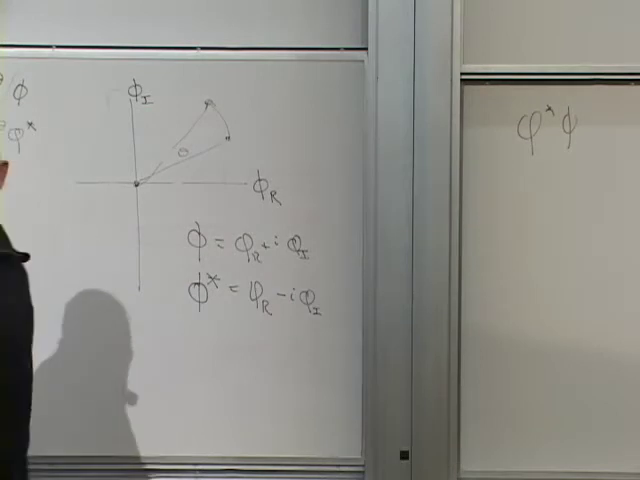
\includegraphics[width=0.80\textwidth]{lecture_07_figure_02.png}
\caption{內部 \((\phi_R,\phi_I)\) 平面上的複數場。黑板上列出 \(\phi\) 和 \(\phi^*\) 的分解，以及不變半徑 \(\phi^*\phi\)。}
\lectureframe{00:33:33}
\end{figure}

採用以下拉格朗日量：
\begin{equation}
  \mathcal L
  =\partial_\mu\phi^*\,\partial^\mu\phi
   -V(\phi^*\phi).
  \label{eq:l07-complex-lagrangian}
\end{equation}
對複數場而言，不需要通常會出現的因子 \(1/2\)，因為這一個乘積已經包含兩個實分量的動能項。變換
\begin{equation}
  \phi'(x)=e^{i\theta}\phi(x),
  \qquad
  \phi^{*\prime}(x)=e^{-i\theta}\phi^*(x)
  \label{eq:l07-global-u1}
\end{equation}
會將每個場值都旋轉相同的角度。此處的 \(\theta\) 在空間和時間中都是常數。撇號表示變換後的場，不是導數。

由於 \(\theta\) 是常數，
\begin{equation}
  \partial_\mu\phi'=e^{i\theta}\partial_\mu\phi,
  \qquad
  \partial_\mu\phi^{*\prime}
  =e^{-i\theta}\partial_\mu\phi^*.
\end{equation}
動能項中的相位會相消，而且
\(\phi^{*\prime}\phi'=\phi^*\phi\)。因此，任何只依賴 \(\phi^*\phi\) 的勢都具有相同的對稱性。若有項只依賴 \(\phi_R\)，就會在內部平面中選定一個方向，造成顯式對稱性破缺。

\subsection{單一極小值與一圈極小值}

對稱勢在性質上有兩種截然不同的情況。第一種的唯一極小值在原點，例如
\begin{equation}
  V_{\rm unbroken}=m^2\phi^*\phi,
  \qquad m^2>0.
\end{equation}
它的圖形是旋轉對稱的拋物面。真空 \(\phi=0\) 在任意旋轉下都保持不變，因此對稱性沒有破缺。

現在改選
\begin{equation}
  V_{\rm broken}
  =-a\,\phi^*\phi+b(\phi^*\phi)^2,
  \qquad a,b>0.
  \label{eq:l07-mexican-hat}
\end{equation}
負的二次項會使場離開原點，正的四次項則阻止場趨向無窮大。令 \(r^2=\phi^*\phi\)，極小化後得到
\begin{equation}
  \frac{dV}{d(r^2)}=-a+2br^2=0,
  \qquad
  r^2=f^2=\frac{a}{2b}.
  \label{eq:l07-vacuum-radius}
\end{equation}
因此，極小值構成一個圓。勢能完全具有旋轉對稱性，但均勻基態仍必須在圓上選定一點。

\begin{figure}[htbp]
\centering
\includegraphics[width=0.72\textwidth]{lecture_07_figure_06.png}
\caption{將對稱性破缺的勢能畫成旋轉曲面。原點不穩定，簡併極小值則構成環形谷底。}
\lectureframe{00:37:25}
\end{figure}

可以把場想成普通空間每一點上的一支小箭頭，箭頭位於這個內部平面中。勢能要求每支箭頭的長度都是 \(f\)。梯度能則要求相鄰箭頭的方向幾乎相同。因此，基態在各處都有相同的角度，但定律並未偏好任何特定角度。這就是連續對稱性的自發破缺。

\section{從疇壁到平滑扭轉}

再做一次邊界實驗。在左邊界把場固定於一個真空點 \(A\)，在右邊界則固定於另一個真空點 \(B\)。若場局部跳變，梯度就會很大。然而，不同於離散對稱性的情形，場可以沿著圓連續變化，同時始終留在勢能的谷底。

在低能情況下，將場寫成 \(\phi=f e^{i\alpha(x)}\)。在一維空間中，相關的能量為
\begin{equation}
  E[\alpha]
  =f^2\int_0^L dx\,\left(\frac{d\alpha}{dx}\right)^2.
  \label{eq:l07-angle-functional}
\end{equation}
固定兩端的角度後，變分可得
\begin{equation}
  \frac{d^2\alpha}{dx^2}=0,
  \qquad
  \alpha(x)=\alpha_A+
    \frac{\alpha_B-\alpha_A}{L}\,x.
  \label{eq:l07-linear-twist}
\end{equation}
最佳構型會將扭轉均勻地分布在整個樣品中。它的能量按下式變化：
\begin{equation}
  E_{\rm twist}
  =f^2\frac{(\alpha_B-\alpha_A)^2}{L},
  \label{eq:l07-twist-energy}
\end{equation}
因此，只要增加 \(L\)，能量就可以任意小。

\begin{figure}[htbp]
\centering
\begin{adjustbox}{max width=\linewidth}
\begin{tikzpicture}[x=0.95cm,y=0.95cm]
  \begin{scope}
    \draw[->] (0,0) -- (6.2,0) node[right] {$x$};
    \draw[->] (0,0) -- (0,3.5) node[above] {$\alpha(x)$};
    \draw[very thick,blue!70!black] (0.45,0.65) -- (5.7,2.85);
    \fill (0.45,0.65) circle (1.8pt) node[left] {$\alpha_A$};
    \fill (5.7,2.85) circle (1.8pt) node[right] {$\alpha_B$};
    \node at (3.1,-0.65) {physical space};
  \end{scope}
  \begin{scope}[xshift=9.2cm,yshift=1.65cm]
    \draw[thick] (0,0) circle (1.8);
    \fill (1.55,-0.92) circle (1.8pt) node[below right] {$A$};
    \fill (-0.45,1.74) circle (1.8pt) node[above] {$B$};
    \draw[very thick,blue!70!black,-{Latex[length=2.5mm]}]
      (1.55,-0.92) arc[start angle=-31,end angle=104,radius=1.8];
    \node at (0,-2.35) {vacuum circle};
  \end{scope}
\end{tikzpicture}
\end{adjustbox}
\caption{同一個低能構型的兩種描述。角度在物理空間中線性變化，而場則沿著真空圓的短弧，在內部空間中變化。}
\end{figure}

\begin{classroomqa}
\audiencequestion{繞著圓有兩條路可走。場會走哪一條？它可能被困在較長的路徑上嗎？
\lecturetimestamp{00:41:54}}
\lecturerresponse{對一般的端點而言，較短的角向路徑梯度較小，因此能量也較低。若兩端點位於直徑兩端，兩條最簡單的路徑便具有相同能量。若透過緩慢移動端點來製備構型，它可能留下額外的繞行，並被困在能障之後；但若給定一對一般端點，沒有額外扭轉的最短路徑才是基態。}
\end{classroomqa}

\begin{classroomqa}
\audiencequestion{路徑能否離開谷底、穿過圓內部，讓整體路程變短？
\lecturetimestamp{00:43:32}}
\lecturerresponse{在低能且樣品夠長的情況下，爬升徑向勢能並不划算。將半徑維持在真空值，並讓角度線性變化，可使有效能量最小；上面的變分計算已顯示這一點。對於具有特定勢能的有限系統，可以同時極小化徑向與角向運動；但戈德斯通結論適用於波長任意長的極限，在此極限下，沿谷底平滑變化的構型能量較低。}
\end{classroomqa}

\begin{classroomqa}
\audiencequestion{如果環形谷底傾斜，使某個角度的能量較低，情況會有什麼變化？
\lecturetimestamp{00:44:33}}
\lecturerresponse{那麼對稱性就會顯式破缺。某一點會成為真正的基態，沿圓周運動也會出現回復力，因此角向激發不再是嚴格無質量的。}
\end{classroomqa}

\section{零動量振盪的能量就是質量}

平滑扭轉揭示了一種能量只來自梯度的場。要了解這為何代表粒子無質量，可以比較相對論性色散關係：
\begin{equation}
  \omega^2=\bm{k}^2+m^2.
  \label{eq:l07-dispersion}
\end{equation}
波 \(e^{i(\bm{k}\cdot\bm{x}-\omega t)}\) 攜帶動量 \(\bm{k}\)。若 \(m=0\)，波長趨近無限大時，能量便趨近於零：\(\omega=|\bm{k}|\to0\)。若 \(m\ne0\)，即使空間均勻的模式 \(\bm{k}=0\)，仍會以頻率 \(\omega=m\) 振盪。質量就是零動量時無法消除的能量。

同樣的差異也能從拉格朗日量看出來。項
\begin{equation}
  -\frac12m^2\varphi^2
\end{equation}
即使場發生均勻位移，也會提供回復力。只有導數項的場則沒有這種回復力：波長愈長，梯度能就愈接近零。

\subsection{極座標變數將兩種模式分開}

將破缺對稱性的複數場寫成
\begin{equation}
  \phi(x)=\rho(x)e^{i\alpha(x)}.
  \label{eq:l07-polar}
\end{equation}
\(\rho\) 和 \(\alpha\) 都是場。微分後得到
\begin{align}
  \partial_\mu\phi
  &=e^{i\alpha}
    \left(\partial_\mu\rho+i\rho\,\partial_\mu\alpha\right),\\
  \partial_\mu\phi^*
  &=e^{-i\alpha}
    \left(\partial_\mu\rho-i\rho\,\partial_\mu\alpha\right).
\end{align}
交叉項會相消，剩下
\begin{equation}
  \partial_\mu\phi^*\,\partial^\mu\phi
  =(\partial_\mu\rho)(\partial^\mu\rho)
   +\rho^2(\partial_\mu\alpha)(\partial^\mu\alpha).
  \label{eq:l07-polar-kinetic}
\end{equation}
由於 \(\phi^*\phi=\rho^2\)，
\begin{equation}
  \mathcal L
  =(\partial\rho)^2+\rho^2(\partial\alpha)^2-V(\rho^2).
  \label{eq:l07-polar-lagrangian}
\end{equation}
勢能中有 \(\rho\)，卻沒有 \(\alpha\)。這正是以最有用的形式呈現該對稱性。

\begin{figure}[htbp]
\centering
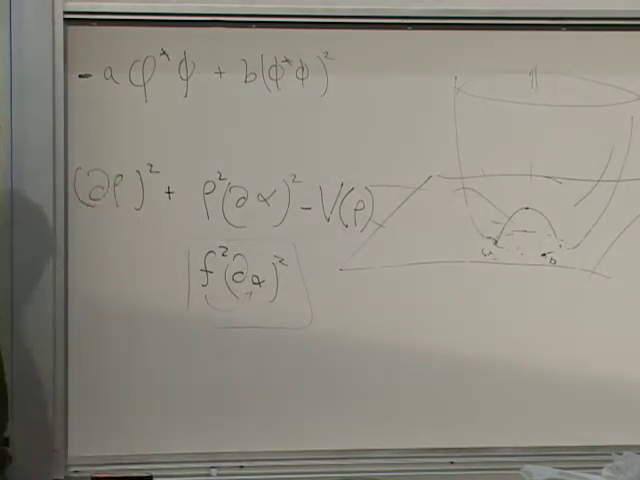
\includegraphics[width=0.88\textwidth]{lecture_07_figure_03.png}
\caption{極座標場的拉格朗日量、框出的低能角向項，以及對稱性破缺勢能。徑向運動會爬升勢能；角向運動則沿著谷底前進。}
\lectureframe{00:56:40}
\end{figure}

對於極低能的激發，場會保持在 \(\rho=f\) 附近。此時
\begin{equation}
  \mathcal L_{\rm angular}
  \simeq f^2(\partial_\mu\alpha)(\partial^\mu\alpha).
\end{equation}
依照因子 \(1/2\) 的選用慣例，定義正則歸一化的角向場為
\begin{equation}
  \beta=\sqrt{2}\,f\alpha,
  \qquad
  \mathcal L_{\rm angular}
  =\frac12(\partial_\mu\beta)(\partial^\mu\beta).
  \label{eq:l07-goldstone-field}
\end{equation}
這裡沒有 \(\beta^2\) 項。這個角向場的量子是無質量的，也就是戈德斯通玻色子。

徑向場的行為則不同。若將 \(\rho\) 從 \(f\) 處處往外移，它會滾回、越過谷底，再繞著谷底振盪。若 \(\rho=f+h\)，將它代入式~\eqref{eq:l07-mexican-hat}展開後可得
\begin{equation}
  V(f+h)=V(f)+\frac12m_h^2h^2+\cdots,
\end{equation}
因此 \(h\) 具有質量。從幾何上看，角向是平坦的，徑向則是彎曲的。

\begin{classroomqa}
\audiencequestion{如果場沿徑向偏離，會直接落回去嗎？接下來會發生什麼？\lecturetimestamp{00:57:10}}
\lecturerresponse{若沒有角向運動，場會朝極小值落下，越過極小值後再作徑向振盪。均勻振盪的空間動量為零，但頻率不為零；這個頻率就是徑向激發的質量。相較之下，均勻的角向位移會落在另一個真空上，沒有回復力。}
\end{classroomqa}

在這個例子中，戈德斯通原理的內容是：自發破缺連續全域對稱性時，真空流形上的每一個獨立平坦方向都會產生一個無質量模式。
\editorialnote{這項說法以相對論場論的通常條件為前提。在非相對論多體系統中，南部--戈德斯通模式的數目和色散關係可能更為微妙；不過，對這個相對論性的\(U(1)\)模型而言，本講關於長波長的結論仍然成立。}

\section{自旋波、弦波與聲波}

這個定理雖然抽象，背後的機制卻很熟悉。在各向同性鐵磁體中，所有自旋一起旋轉並不會改變能量。若取向在樣品中緩慢變化，就會形成自旋波。它的能量代價會隨波數趨近於零，因此它是自旋旋轉對稱性破缺所產生的戈德斯通模式。

長彈性弦則提供另一種圖像。忽略重力，並架設弦的兩端，使整條弦能夠沿垂直方向平移。整條弦均勻地垂直平移不耗能。若平移量沿著弦緩慢改變，就會形成長波長的橫波。原本均勻的對稱操作於是延伸成隨位置緩慢變化的形變。

\begin{figure}[htbp]
\centering
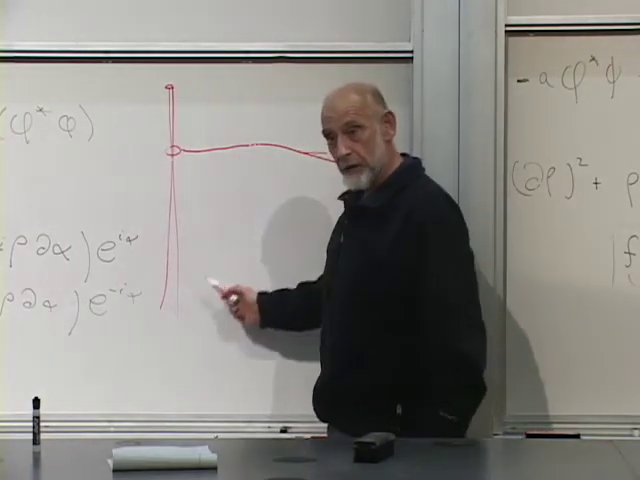
\includegraphics[width=0.68\textwidth]{lecture_07_figure_04.png}
\caption{戈德斯通模式類比中所畫的緩慢變化弦形。物理上的重點是長波長形變的斜率很小，而不是曲線在垂直方向上的位置。}
\lectureframe{01:04:19}
\end{figure}

\begin{classroomqa}
\audiencequestion{弦能否在動量為零時仍帶有振盪能量？\lecturetimestamp{01:04:41}}
\lecturerresponse{必須區分垂直方向的機械動量，以及沿弦傳播的波動動量。駐波可以是 \(+k\) 與 \(-k\) 模式的疊加，因此淨動量為零，但仍然帶有能量。在場論類比中，動量指沿著軸向的波數；垂直位移則代表內部場座標。}
\end{classroomqa}

彈簧玩具可以呈現縱波的情形。將理想化的無限長彈簧玩具沿軸向整體平移，狀態不會改變。若相鄰部分的平移量略有不同，就會形成平緩的壓縮波。在固體或流體中，長波長聲波同樣來自集體位移和密度變化。自旋波、弦的橫波和聲波並不是相同的微觀激發，但它們有一個關鍵共通點：均勻的連續操作不耗能，而緩慢變化的操作則形成軟模式。
\editorialnote{在晶體中，聲學聲子通常被描述為自發破缺連續平移對稱性所產生的南部--戈德斯通模式。講課中以弦和彈簧玩具作為力學類比，說明相同的僅含導數能量結構。}

這些術語很容易混淆，因此課堂上開了個簡短的玩笑：它們是\emph{戈德斯通}玻色子，以 Jeffrey Goldstone 命名，不是規範玻色子。講課中提到 Goldstone 是 Susskind 的朋友，接著便轉向真正不同的主題：規範不變性。

\section{從全域相位對稱性到規範對稱性}

\(U(1)\)相位對稱性在本課程中已經作為與電荷守恆相關的對稱性出現過。帶電粒子的場是複數場，將這樣的場乘上共同相位，不會改變全域理論。為了方便理解，可以把這個電荷想成電荷；不過，它也可能代表其他 \(U(1)\) 量子數。真實的光子是無質量的；我們最終要探討的目標，是像光子一樣的場，例如有質量的 \(Z\)。

新的問題是，
\begin{equation}
  \phi'(x)=e^{i\theta(x)}\phi(x)
  \label{eq:l07-local-u1}
\end{equation}
當 \(\theta\) 在時空中任意變化時，這還能是一種對稱性嗎？函數 \(\theta(x)\) 是變換參數，不是額外的動力學場。我們對它微分，來檢驗這個設想：
\begin{equation}
  \partial_\mu\phi'
  =e^{i\theta}
   \left[\partial_\mu\phi+i(\partial_\mu\theta)\phi\right].
  \label{eq:l07-local-derivative}
\end{equation}
若 \(\theta\) 為常數，就不會出現這個額外項。對共軛場而言，
\begin{equation}
  \partial_\mu\phi^{*\prime}
  =e^{-i\theta}
   \left[\partial_\mu\phi^*-i(\partial_\mu\theta)\phi^*\right].
\end{equation}
兩者相乘後得到
\begin{align}
  \partial_\mu\phi^{*\prime}\partial^\mu\phi'
  ={}&
  \partial_\mu\phi^*\partial^\mu\phi
  i\left(
      \phi\,\partial_\mu\phi^*
      -\phi^*\partial_\mu\phi
    \right)\partial^\mu\theta
  \nonumber\\
  &+\phi^*\phi\,
    \partial_\mu\theta\,\partial^\mu\theta.
  \label{eq:l07-local-failure}
\end{align}
勢能仍保持不變，因為 \(\phi^*\phi\) 不變，但普通的動能項不再保持不變。全域對稱性不會自動成為局域對稱性。

\begin{classroomqa}
\audiencequestion{在墨西哥帽的圖像中，這種不變性失效是否代表環形谷底上有起伏？\lecturetimestamp{01:19:37}}
\lecturerresponse{不是。勢能在角向仍然可以完全平坦。額外的能量代價來自相位在不同時空位置有所差異時產生的梯度。這不是谷底變得凹凸不平，而是普通導數項會感受到空間變化。}
\end{classroomqa}

\subsection{補償用的向量場}

自然界中的 \(W\)、\(Z\) 和膠子交互作用，是由局域規範對稱性組織起來的，不只是由整體變換決定。若要讓局域相位操作成為對稱性，就必須在理論中加入四向量場 \(A_\mu\)。在電磁學中，\(A_0\) 是純量勢，另外三個空間分量則構成向量勢。它們的導數會形成電場和磁場。

採用前後一致的慣例：
\begin{equation}
  \phi'=e^{i\theta}\phi,
  \qquad
  A'_\mu=A_\mu-\partial_\mu\theta,
  \qquad
  D_\mu=\partial_\mu+iA_\mu.
  \label{eq:l07-gauge-convention}
\end{equation}
黑板上檢查抵消時曾改變一個符號；式\eqref{eq:l07-gauge-convention}則將三個符號一併確定。規範耦合和電荷暫時都吸收到 \(A_\mu\) 中。
\editorialnote{若明確寫出電荷 \(q\) 和耦合常數 \(g\)，可以寫成
\(D_\mu=\partial_\mu+igqA_\mu\) 和
\(A'_\mu=A_\mu-(gq)^{-1}\partial_\mu\theta\)。講課中略去這些常數，讓抵消關係更清楚。}

對共軛場而言，
\begin{equation}
  D_\mu\phi^*=\partial_\mu\phi^*-iA_\mu\phi^*.
\end{equation}
現在
\begin{align}
  D'_\mu\phi'
  &=
  \left(\partial_\mu+iA'_\mu\right)e^{i\theta}\phi
  \nonumber\\
  &=
  e^{i\theta}
  \left[
    \partial_\mu\phi+i(\partial_\mu\theta)\phi
    +i(A_\mu-\partial_\mu\theta)\phi
  \right]
  \nonumber\\
  &=e^{i\theta}D_\mu\phi.
  \label{eq:l07-covariant-transform}
\end{align}
\(\theta\) 的多餘導數項會由 \(A_\mu\) 的變換抵消。同樣地，
\begin{equation}
  D'_\mu\phi^{*\prime}=e^{-i\theta}D_\mu\phi^*.
\end{equation}
兩者相乘後保持不變。「\emph{協變}」的意思是，導數的變換方式與場本身相同而簡單。

\section{規範場的動力學}

若引入 \(A_\mu\) 只是為了修正導數，它本身就不會有動力學。規範不變的場強為
\begin{equation}
  F_{\mu\nu}
  =\partial_\mu A_\nu-\partial_\nu A_\mu.
  \label{eq:l07-field-strength}
\end{equation}
它是反對稱的，因此 \(F_{\mu\mu}=0\)。它的時間--空間分量包含電場，空間--空間分量則包含磁場。用熟悉的三維向量表示法來說，電磁場的能量密度正比於 \(\bm E^2+\bm B^2\)，而洛侖茲形式的拉格朗日量正比於 \(\bm E^2-\bm B^2\)；正負號取決於度規慣例。

\begin{classroomqa}
\audiencequestion{電磁場的能量和拉格朗日量分別是什麼？\lecturetimestamp{01:33:20}}
\lecturerresponse{能量由 \(E^2+B^2\) 組成；拉格朗日量則使用 \(E^2-B^2\)。以協變形式表示，後者通常寫成 \(F_{\mu\nu}F^{\mu\nu}\) 的倍數。反對稱張量就是向量勢的四維旋度。}
\end{classroomqa}

場強本身也具有規範不變性：
\begin{align}
  F'_{\mu\nu}
  &=
  \partial_\mu(A_\nu-\partial_\nu\theta)
  -\partial_\nu(A_\mu-\partial_\mu\theta)
  \nonumber\\
  &=
  F_{\mu\nu}
  -\partial_\mu\partial_\nu\theta
  +\partial_\nu\partial_\mu\theta
  =F_{\mu\nu}.
  \label{eq:l07-field-strength-invariant}
\end{align}
最後一個等號成立，是因為普通的混合偏導數可以交換次序。因此，標準的規範不變拉格朗日量可以寫成
\begin{equation}
  \boxed{
  \mathcal L
  =(D_\mu\phi)^*D^\mu\phi
  -V(\phi^*\phi)
  -\frac14F_{\mu\nu}F^{\mu\nu}}
  \label{eq:l07-scalar-qed}
\end{equation}
至於正負號與歸一化慣例，則取決於所採用的度規。

\begin{figure}[htbp]
\centering
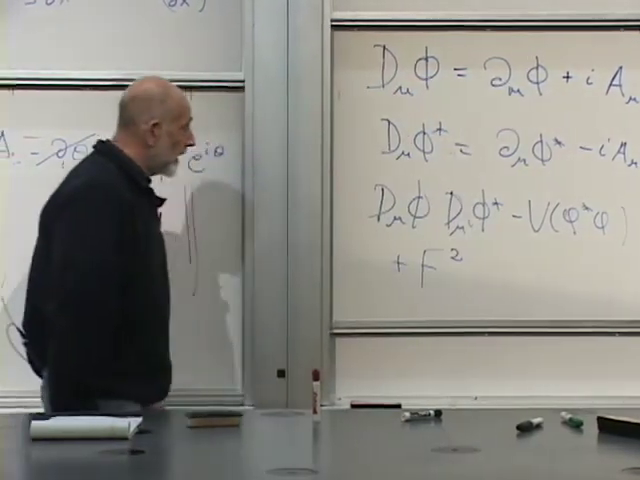
\includegraphics[width=0.84\textwidth]{lecture_07_figure_05.png}
\caption{黑板上的協變導數，以及組合完成的規範不變拉格朗日量。為了清楚呈現變換結構，黑板上的寫法省略了數值因子。}
\lectureframe{01:38:45}
\end{figure}

這個構造將全域 \(U(1)\) 對稱性推廣成局域對稱性，但代價---或者從物理角度來看，這份收穫---是引入一個新的向量場。在阿貝爾例子中，這個場就是電磁勢。

\begin{classroomqa}
\audiencequestion{我們一開始的拉格朗日量使用普通導數。為什麼可以把它們換成協變導數，並把換過之後的結果稱為真正的理論？\lecturetimestamp{01:42:55}}
\lecturerresponse{我們正在構造一個不同且擴充過的理論：帶電物質加上規範場。局域規範不變性決定了兩者的耦合方式。由此得到的量子理論在數學上自成一套一致的結構，也符合自然界對光子和弱作用規範場的組織方式。若不一致地耦合相對論性向量場，可能會引入非物理極化態並破壞機率守恆，因此規範原理並非只是把舊有的自由標量理論重新包裝。}
\end{classroomqa}

\begin{classroomqa}
\audiencequestion{所以，加入新場就是這項修改的根本理由嗎？\lecturetimestamp{01:44:57}}
\lecturerresponse{是的。沒有\(A_\mu\)時，局域轉動後的場，其導數會含有一個未被抵消的\(\partial_\mu\theta\)。加入\(A_\mu\)及其變換律後，這個項就能抵消。用幾何語言來說，\(A_\mu\)是叢上的聯絡；這套更深層的數學確實有其意義，也很有用，但上面的代數已涵蓋此處所需的部分。}
\end{classroomqa}

\section{為什麼裸規範玻色子質量會被禁止}

對一般的玻色場而言，質量以二次項表示。很容易讓人想加上
\begin{equation}
  \Delta\mathcal L_{\rm Proca}
  =\frac12m^2A_\mu A^\mu.
  \label{eq:l07-proca}
\end{equation}
但在\(A_\mu\mapsto A_\mu-\partial_\mu\theta\)之下，
\begin{equation}
  A'_\mu A^{\mu\prime}
  =
  A_\mu A^\mu
  -2A^\mu\partial_\mu\theta
  +\partial_\mu\theta\,\partial^\mu\theta,
\end{equation}
因此，式~\eqref{eq:l07-proca}並非規範不變。我們不能在保留局域對稱性的同時，任意將質量項加進這個規範理論。

\begin{figure}[htbp]
\centering
\includegraphics[width=0.72\textwidth]{lecture_07_figure_07.png}
\caption{所提議的裸向量質量項為\(\tfrac12m^2A_\mu A^\mu\)。此項在\(A_\mu\mapsto A_\mu-\partial_\mu\theta\)之下不再保持不變，這正是希格斯機制所要克服的障礙。}
\lectureframe{01:39:48}
\end{figure}

這就是表面上的僵局。規範不變性說明了光子為何無質量，也保護理論不受非物理自由度的影響；然而，\(W\)和\(Z\)卻有質量。解決之道不能是顯式加入向量質量項，而必須來自規範不變拉格朗日量中原有的場。

\begin{classroomqa}
\audiencequestion{引入規範不變性本身會產生戈德斯通玻色子嗎？\lecturetimestamp{01:45:51}}
\lecturerresponse{不會。向量勢引入之前，連續的\emph{整體}對稱性自發破缺時，就已經產生了戈德斯通玻色子。對稱性一旦成為局域對稱性，相位的變化就可以由\(A_\mu\)補償。在對稱性破缺的規範理論中，角向模式不再是獨立的無質量粒子；它提供了如今有質量的向量場所需的額外極化。下一講將推導這個結果，而不只把它說出來。}
\end{classroomqa}

\begin{classroomqa}
\audiencequestion{這些內容能解釋河流為什麼蜿蜒嗎？\lecturetimestamp{01:47:03}}
\lecturerresponse{目前沒有已知的直接關聯。流體渦旋乃至生物體的形狀，當然都可以用對稱性方法描述；在意想不到的地方發現場論思想，也不值得驚訝。不過，本講並未主張存在描述河流蜿蜒的規範理論。}
\end{classroomqa}

\section{本講到此為止}

我們現在已經具備了開頭所承諾的兩個要素。具有一圈真空態的連續整體對稱性，會有一個平坦的角向方向；這個方向的緩慢變化就是無質量的戈德斯通場。局域對稱性則要求引入規範聯絡與協變導數，並禁止式~\eqref{eq:l07-proca}中的直接向量質量項。

下一步是將式~\eqref{eq:l07-mexican-hat}中的破缺勢，放進式~\eqref{eq:l07-scalar-qed}所描述的規範不變理論中。接著會有兩件事同時發生：獨立的戈德斯通粒子從物理譜中消失，而向量場獲得質量。按照一般的教學說法，規範對稱性自發破缺了；更精確地說，規範冗餘仍然存在，而理論進入希格斯相，其中有一個有質量的向量激發。\editorialnote{局域規範對稱性是描述上的冗餘，不是作用於不同可觀測態之間的一般物理對稱性。本講採用「規範對稱性自發破缺」這個標準簡稱。規範不變的物理陳述則是：希格斯相中的自由度重新組合。}

這就是希格斯現象。我們還沒有推導它。本講完成了必要而更為困難的工作，讓問題變得足夠精確；如此一來，解答出現時便勢所必然。

\chapter{希格斯機制：規範玻色子如何獲得質量}

現在我們把上一講介紹的兩個想法結合起來。具有破缺全域 \(U(1)\) 對稱性的複純量場，包含一個有質量的徑向振盪，以及一個無質量的角向振盪。局域不變的 \(U(1)\) 理論則包含一個無質量的規範場。當純量帶電，且其平衡幅值不為零時，這兩項陳述不能直接併在一起。角向模態與規範場結合：規範場因此有了質量，表面上的戈德斯通玻色子不再是獨立粒子，而徑向的希格斯模態仍然存在。

我們會以光子作為模型中的規範玻色子，但這不是我們要得出的物理結論。真空中的電磁 \(U(1)\) 並未破缺，因此真實的光子是無質量的。同一機制作用於電弱理論中的 \(W^\pm\) 和 \(Z\)；在該理論中，規範群和純量多重態都更為複雜。阿貝爾模型能清楚呈現這個機制，不會讓群論掩蓋它。

\begin{classroomqa}
\audiencequestion{先前的討論是否表示希格斯機制會賦予真實光子質量？\lecturetimestamp{00:00:23}}
\lecturerresponse{不會。我們問的是，\emph{如果}與光子相關的 \(U(1)\) 處於破缺相，會發生什麼事。那個假想的光子會變得有質量。真實的電磁真空並不處於該相；在粒子物理中的應用，指的是 \(W\) 和 \(Z\) 的質量。}
\end{classroomqa}

與電荷守恆相關的對稱性是相位旋轉
\begin{equation}
  \phi(x)\longmapsto e^{i\theta}\phi(x),
\end{equation}
這是一種稱為 \(U(1)\) 的內部旋轉。超導體提供了破缺相的實際類比。在超導體內部，電磁場有有限的穿透深度，在重要的方面表現得像有質量的場；在超導體外部，普通的無質量光子則重新出現。

\section{場的質量代表什麼}

\subsection{色散關係與零動量能隙}

在引入希格斯場之前，值得先明確說明我們所說的質量究竟是什麼意思。對波而言，
\begin{equation}
  E=\hbar\omega,
  \qquad
  p=\hbar k,
  \label{eq:l08-quantum-wave}
\end{equation}
因此，\((E,p)\) 圖和 \((\omega,k)\) 圖所含的資訊相同，只差了 \(\hbar\) 的因子。在真空中，無質量的相對論性激發滿足
\begin{equation}
  E=c|p|,
  \qquad
  \omega=c|k|.
  \label{eq:l08-massless-dispersion}
\end{equation}
\(k\) 的正負號代表相反的傳播方向。關鍵在於，\(\omega\) 會隨著 \(k\) 趨近於零。

有質量的相對論性粒子滿足
\begin{equation}
  E^2=c^2p^2+m^2c^4.
  \label{eq:l08-massive-dispersion}
\end{equation}
在單位制 \(c=\hbar=1\) 下，
\begin{equation}
  \omega^2=k^2+m^2.
\end{equation}
當 \(k=0\) 時，能量為 \(E=mc^2\)；以自然單位制表示，就是 \(m\)。因此，質量就是零動量模態具有的非零能隙。

\begin{figure}[htbp]
\centering
\begin{adjustbox}{max width=\linewidth}
\begin{tikzpicture}[x=1.05cm,y=1.05cm]
  \begin{scope}
    \draw[->] (-0.2,0) -- (4.2,0) node[right] {\(k\)};
    \draw[->] (0,-0.2) -- (0,3.1) node[above] {\(\omega\)};
    \draw[very thick,blue!65!black] (0,0) -- (3.8,2.75);
    \draw[very thick,orange!70!black] (0,0) -- (3.8,1.75);
    \node[blue!65!black,rotate=36] at (2.65,2.15)
      {\(\omega=c_{\rm vac}k\)};
    \node[orange!70!black,rotate=24] at (2.65,1.05)
      {ordinary medium};
    \node[below] at (2,-0.45) {gapless};
  \end{scope}
  \begin{scope}[xshift=6.2cm]
    \draw[->] (-0.2,0) -- (4.2,0) node[right] {\(k\)};
    \draw[->] (0,-0.2) -- (0,3.1) node[above] {\(\omega\)};
    \draw[very thick,domain=0:3.8,samples=120,smooth,teal!70!black]
      plot (\x,{sqrt(0.9+0.45*\x*\x)});
    \draw[dashed] (0,0.95) -- (1.0,0.95);
    \node[left] at (0,0.95) {\(m\)};
    \node[teal!70!black] at (2.55,2.15)
      {\(\omega^2=k^2+m^2\)};
    \node[below] at (2,-0.45) {gapped};
  \end{scope}
\end{tikzpicture}
\end{adjustbox}
\caption{改變傳播速度會改變無能隙色散關係的斜率；賦予激發質量，則會在 \(k=0\) 處形成非零能隙。}
\label{fig:l08-dispersion}
\end{figure}

普通透明材料可以降低波的相速度，卻不會因此形成這種相對論性的質量能隙。在介面上，入射波的頻率固定，波數則會依照介質的色散關係調整。改變斜率與抬高截距並不相同。
\editorialnote{材料可能有多個電磁分支，而電漿或共振介質可能具有非零的電漿頻率能隙。本講比較的特定對象，是普通折射分支與超導響應。更一般地說，無能隙表示當 \(k\to0\) 時，\(\omega(k)\to0\)；在非相對論介質中，並非每種情況都必須嚴格線性。}

\begin{classroomqa}
\audiencequestion{光子只要穿過物質，例如稜鏡，就會獲得質量嗎？\lecturetimestamp{00:03:02}}
\lecturerresponse{不會。折射可以改變頻率與波數的關係，因而改變傳播速度，但該分支仍會在 \(\omega=0\) 處通過，且此時 \(k=0\)。超導相則會使電磁響應具有有限的穿透深度倒數，這是質量的類比。}
\end{classroomqa}

\begin{classroomqa}
\audiencequestion{固定頻率的光進入玻璃時，改變的是波數嗎？\lecturetimestamp{00:09:20}}
\lecturerresponse{是。靜止介面具有時間平移不變性，因此頻率維持不變。玻璃中的色散曲線斜率不同，所以相同的 \(\omega\) 對應不同的 \(k\)，波長也因此不同。}
\end{classroomqa}

斜率
\begin{equation}
  v_g=\frac{d\omega}{dk}
\end{equation}
是波包的群速度。如果斜率隨 \(k\) 改變，不同的傅立葉分量就會以不同速度移動，波包也會發生色散。這就是為什麼關係式 \(\omega(k)\) 稱為\emph{色散關係}。

\begin{classroomqa}
\audiencequestion{這條曲線叫什麼？它的斜率代表什麼？\lecturetimestamp{00:11:02}}
\lecturerresponse{這條曲線是色散關係，其導數
\(d\omega/dk\) 就是群速度。斜率固定時，各種波長的波以相同速度傳播；斜率變化時，波包便會展開。就目前的討論而言，關鍵差別在於曲線是否通過原點，或是具有能隙。}
\end{classroomqa}

\subsection{均勻振盪對應於靜止粒子}

\(k=0\) 模態的波長無限長：場在各處都偏移相同的量。讓均勻偏移開始振盪。如果場以非零頻率振盪，相應的量子便有非零靜止能量，也就是有質量。如果該方向沒有回復力，頻率就會是零，模態也就是無質量的。

這是經典的陳述，不要求空間上彼此分離的粒子處於量子疊加態。均勻的經典場組態，只是在整個空間中重複同一個場值。

\begin{classroomqa}
\audiencequestion{如果整個場一起偏移，這和量子糾纏是同一回事嗎？\lecturetimestamp{00:10:04}}
\lecturerresponse{不是。均勻的經典場是單一的經典組態。糾纏關聯的是不同的量子可能狀態，例如自旋向上--向下與自旋向下--向上的組態。在許多位置準備相同的場值，本身並不構成糾纏，也不代表存在瞬時的因果作用。}
\end{classroomqa}

對於正則歸一化的實場，
\begin{equation}
  \mathcal L
  =\frac12\partial_\mu\varphi\,\partial^\mu\varphi-V(\varphi),
\end{equation}
在平衡點 \(\varphi_0\) 附近展開：
\begin{equation}
  V(\varphi_0+\eta)
  =V(\varphi_0)
   +\frac12V''(\varphi_0)\eta^2+\cdots.
\end{equation}
線性項在極小值處消失，而場方程給出
\begin{equation}
  \omega^2=\bm{k}^2+m^2,
  \qquad
  m^2=V''(\varphi_0).
  \label{eq:l08-curvature-mass}
\end{equation}
因此，質量是勢能沿運動方向的曲率。平坦方向的曲率為零，因而產生無質量模態。

\section{破缺的複純量}

\subsection{徑向與角向運動}

將複純量以直角座標和極座標表示：
\begin{equation}
  \phi=\phi_R+i\phi_I=\rho e^{i\alpha},
  \qquad
  \phi^*=\phi_R-i\phi_I=\rho e^{-i\alpha}.
  \label{eq:l08-polar-field}
\end{equation}
複平面是一個\emph{內部}場空間。在每個物理時空點 \(x\)，這一對
\((\phi_R(x),\phi_I(x))\) 指定內部平面中的一個點。內部平面的兩個軸都不是實驗室中的空間方向。

\begin{figure}[htbp]
\centering
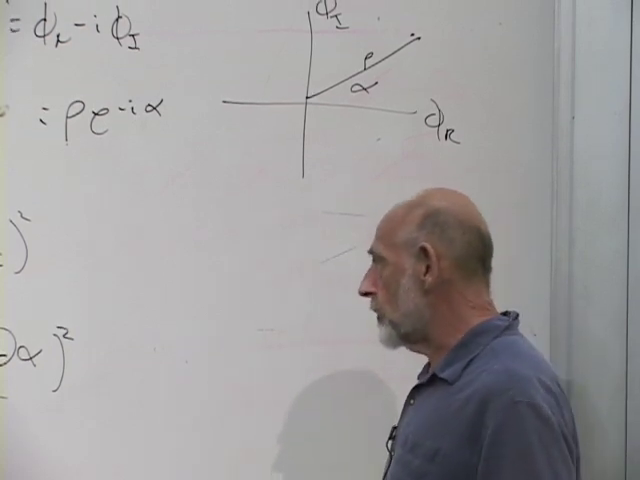
\includegraphics[width=0.72\textwidth]{lecture_08_figure_02.png}
\caption{複純量在內部 \((\phi_R,\phi_I)\) 平面上的表示。半徑為 \(\rho\)，\(\alpha\) 則是內部相位。}
\lectureframe{00:24:41}
\label{fig:l08-internal-plane}
\end{figure}

純量的動能項變為
\begin{align}
  \partial_\mu\phi^*\,\partial^\mu\phi
  &=
  \partial_\mu\phi_R\,\partial^\mu\phi_R
  +\partial_\mu\phi_I\,\partial^\mu\phi_I
  \notag\\
  &=
  \partial_\mu\rho\,\partial^\mu\rho
  +\rho^2\partial_\mu\alpha\,\partial^\mu\alpha.
  \label{eq:l08-polar-kinetic}
\end{align}
全域 \(U(1)\) 不變的勢能取決於 \(\phi^*\phi=\rho^2\)，而不取決於 \(\alpha\)。例如，
\begin{equation}
  V(\phi)
  =\lambda\left(\phi^*\phi-\frac{f^2}{2}\right)^2,
  \qquad \lambda>0.
  \label{eq:l08-mexican-hat}
\end{equation}
勢能的極小值構成一個圓。定律在共同的相位旋轉下保持不變，但選定一個平衡相位，就等於選定圓上的一個點。

\begin{figure}[htbp]
\centering
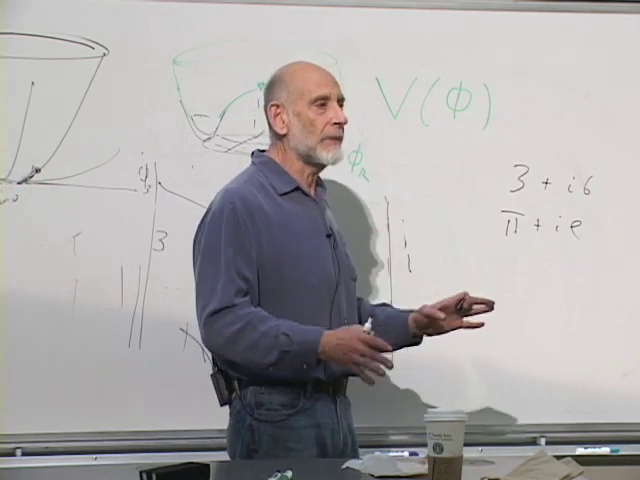
\includegraphics[width=0.78\textwidth]{lecture_08_figure_03.png}
\caption{黑板上的徑向勢能示意圖。勢能在內部場值旋轉下保持對稱，即使場本身不一定位於原點。}
\lectureframe{00:34:22}
\label{fig:l08-radial-potential-board}
\end{figure}

\begin{figure}[htbp]
\centering
\begin{tikzpicture}[x=0.94cm,y=0.94cm]
  \draw[->] (-4.2,0) -- (4.4,0) node[right] {\(\phi_R\)};
  \draw[->] (0,-3.7) -- (0,3.9) node[above] {\(\phi_I\)};
  \draw[very thick,blue!65!black] (0,0) circle (2.45);
  \draw[->,very thick,orange!75!black] (0,0) -- (2.2,1.08);
  \draw[->,very thick,teal!70!black]
    (2.2,1.08) arc[start angle=26,end angle=67,radius=2.45];
  \node[orange!75!black,below right] at (1.15,0.52)
    {radial \(h\): massive};
  \node[teal!70!black,above right] at (1.78,1.76)
    {angular \(\pi\): massless};
  \fill (2.2,1.08) circle (2pt);
  \node[below] at (0,-2.65) {degenerate vacuum circle};
\end{tikzpicture}
\caption{全域對稱性破缺後的理論，在垂直於真空圓的方向上有曲率，沿著圓周的方向則沒有曲率。徑向希格斯模態有質量；角向戈德斯通模態無質量。}
\label{fig:l08-radial-angular}
\end{figure}

令
\begin{equation}
  \phi(x)=\frac{f+h(x)}{\sqrt2}
           e^{i\pi(x)/f}.
  \label{eq:l08-canonical-polar}
\end{equation}
在選定的真空附近，\(h\)表示徑向位移，\(\pi\)則以正則量綱表示切向位移。代入式~\eqref{eq:l08-polar-kinetic}，得到
\begin{equation}
  \partial_\mu\phi^*\,\partial^\mu\phi
  =
  \frac12(\partial_\mu h)^2
  +\frac12\left(1+\frac{h}{f}\right)^2
            (\partial_\mu\pi)^2.
  \label{eq:l08-global-expanded}
\end{equation}
式~\eqref{eq:l08-mexican-hat}的勢能給出
\begin{equation}
  m_h^2=2\lambda f^2,
  \qquad
  m_\pi^2=0.
  \label{eq:l08-global-masses}
\end{equation}
在遠低於 \(m_h\) 的能量下，徑向運動所需的能量很高，因此我們可以暫時固定 \(h=0\)。剩下的拉格朗日量只含有 \(\frac12(\partial\pi)^2\)，沒有 \(\pi^2\) 項。這就是戈德斯通玻色子。\editorialnote{口頭說明有兩處把名稱顛倒，並說是戈德斯通玻色子被吸收後，希格斯玻色子才有質量。黑板上的計算以及本講其餘內容表明，正確的結果是：徑向曲率已使希格斯模態具有質量，而規範玻色子吸收戈德斯通模態後變得有質量。}

\begin{classroomqa}
\audiencequestion{這是標準模型中唯一的自發對稱性破缺嗎？\lecturetimestamp{00:16:39}}
\lecturerresponse{與此處相關且已確立的對稱性破缺機制，是電弱希格斯相。其實際對稱性是 \(SU(2)_L\times U(1)_Y\)，而非單一的 \(U(1)\)；QCD 也有其他真空結構，例如手徵對稱性破缺。這個阿貝爾例子是刻意簡化的規範玻色子機制模型。}
\end{classroomqa}

\begin{classroomqa}
\audiencequestion{希格斯會賦予所有粒子質量嗎？它自己也包括在內嗎？\lecturetimestamp{00:17:11}}
\lecturerresponse{這個問題需要分兩方面回答。電弱對稱性禁止 \(W\)、\(Z\) 和標準模型費米子具有裸質量；它們的質量是在希格斯場取得非零平衡幅值後才出現。徑向希格斯模態的質量來自希格斯場自身勢能的曲率。其他假想粒子則可能具有對稱性所允許、與此機制無關的質量。}
\end{classroomqa}

本講將這類對稱性允許的質量，與可能非常重而難以觀測的粒子聯繫起來，並以暗物質作為可能的例子。這只是提出問題的動機，並非對質量的預測。
\editorialnote{暗物質的質量尺度仍然未知。本講提到粒子質量約為質子質量一千倍，這是過去的推測，並非經實驗確立的暗物質性質。}

\begin{classroomqa}
\audiencequestion{\(\rho\)是物理半徑，還是場值？究竟什麼具有徑向對稱性？\lecturetimestamp{00:33:08}}
\lecturerresponse{在每個時空點，場值都是輔助複平面中的一個點，而 \(\rho=|\phi|\) 是該點到原點的距離。\emph{勢能}在這個內部平面上具有徑向對稱性：所有 \(\rho\) 相同的點，其勢能也相同。這個半徑不是普通空間中的距離。}
\end{classroomqa}

\begin{classroomqa}
\audiencequestion{如果徑向踢動足夠劇烈，能否讓場越過中央極大值，到達勢能的另一側？
\lecturetimestamp{00:36:00}}
\lecturerresponse{原則上，局部組態若有足夠能量，就能越過位能障壁。要讓均勻的宏觀場越過障壁，需要極大的能量；一般的劇烈擾動也會把能量分散到許多場模態中，不會相干地抵達另一側的點。低能近似會固定 \(\rho\)，正是因為在該近似適用的能量範圍內，無法進行這種徑向偏移。}
\end{classroomqa}

\section{為什麼複平面不是時空}

物理座標與內部座標的區別，值得像本講那樣特別停下來說明。純量場之所以稱為純量，是因為它在物理座標軸旋轉時保持不變。兩個實純量場 \(\phi_R(x)\) 和 \(\phi_I(x)\) 在這種旋轉下仍是兩個純量。我們可以把它們合寫成一個複數，但這種記號安排不會使它們變成空間向量的分量。

全域 \(U(1)\) 變換會旋轉場的 \emph{值}：
\begin{equation}
\begin{aligned}
  \phi(x)&\longmapsto e^{i\theta}\phi(x),
  \\
  \rho(x)&\longmapsto\rho(x),
  \\
  \alpha(x)&\longmapsto\alpha(x)+\theta.
\end{aligned}
  \label{eq:l08-global-shift}
\end{equation}
同一個常數 \(\theta\) 用於每個時空點，因此 \(\partial_\mu\alpha\) 保持不變。勢能和一般的動能項都具有這項對稱性。一旦允許 \(\theta\) 隨 \(x\) 改變，導數就會察覺這項變化，論證也就不同了。

\section{將相位旋轉改為局域變換}

\subsection{一般導數不再適用}

令
\begin{equation}
  \phi'(x)=e^{i\theta(x)}\phi(x).
  \label{eq:l08-local-phase}
\end{equation}
則
\begin{equation}
  \partial_\mu\phi'
  =e^{i\theta}
    \left(\partial_\mu\phi+i\,\partial_\mu\theta\,\phi\right).
  \label{eq:l08-ordinary-derivative-fails}
\end{equation}
其中與 \(\partial_\mu\theta\) 成正比的額外項，使 \(\partial_\mu\phi\) 不會像 \(\phi\) 那樣變換。因此，\(\partial_\mu\phi^*\partial^\mu\phi\) 並非在任意局域相位旋轉下都保持不變。

\begin{figure}[htbp]
\centering
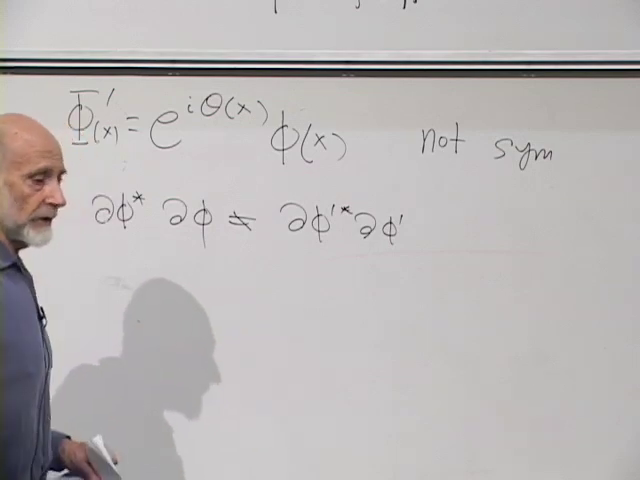
\includegraphics[width=0.78\textwidth]{lecture_08_figure_04.png}
\caption{黑板記下局域相位變換，以及一般導數項無法維持不變的情形。}
\lectureframe{00:46:49}
\label{fig:l08-local-not-symmetry}
\end{figure}

引入一個向量勢，並一致採用以下約定：
\begin{equation}
  D_\mu=\partial_\mu+i g A_\mu,
  \qquad
  A_\mu'=A_\mu-\frac1g\partial_\mu\theta.
  \label{eq:l08-covariant-convention}
\end{equation}
此時
\begin{align}
  D_\mu'\phi'
  &=
  \left(\partial_\mu+i g A_\mu'\right)
  e^{i\theta}\phi
  \notag\\
  &=
  e^{i\theta}
  \left[
    \partial_\mu\phi+i(\partial_\mu\theta)\phi
    +i g A_\mu\phi-i(\partial_\mu\theta)\phi
  \right]
  \notag\\
  &=e^{i\theta}D_\mu\phi.
  \label{eq:l08-covariant-transform}
\end{align}
不需要的項便會互相抵消。共軛導數為
\begin{equation}
  (D_\mu\phi)^*
  =(\partial_\mu-i g A_\mu)\phi^*,
\end{equation}
兩者的相位相反，因此在乘積中會抵消：
\begin{equation}
  (D_\mu\phi)^*D^\mu\phi.
\end{equation}

\begin{classroomqa}
\audiencequestion{上一講寫出的規範場變換，符號是否相反？\lecturetimestamp{00:48:04}}
\lecturerresponse{同時反轉 \(D_\mu\) 的符號和變換律中的符號，只是採用不同的約定。在 \(D_\mu=\partial_\mu+i gA_\mu\) 和 \(\phi'=e^{i\theta}\phi\) 的約定下，為保持一致，必須有 \(A_\mu'=A_\mu-g^{-1}\partial_\mu\theta\)。只要所有符號一起改變，另一種約定也同樣成立。}
\end{classroomqa}

\begin{classroomqa}
\audiencequestion{黑板上 \(\phi\) 的大寫或小寫寫法，是否代表不同的場？\lecturetimestamp{00:55:02}}
\lecturerresponse{這裡沒有要區分兩者。字母形狀不同只是手寫造成的，並不表示有額外的運算或第二個純量。真正有意義的區別是撇號、複共軛星號和時空指標。}
\end{classroomqa}

\begin{classroomqa}
\audiencequestion{動能項中的複共軛，和洛倫茲指標的升降是同一種運算嗎？
\lecturetimestamp{00:56:50}}
\lecturerresponse{不是。星號表示對內部的複數場取共軛。洛倫茲指標則以時空度規升降：\(D^\mu=g^{\mu\nu}D_\nu\)。要得到洛倫茲純量，必須作縮併 \((D_\mu\phi)^*D^\mu\phi\)。這兩種運算都會出現，但用途不同。}
\end{classroomqa}

\subsection{規範場也有自身的動力學}

場強
\begin{equation}
  F_{\mu\nu}=\partial_\mu A_\nu-\partial_\nu A_\mu
  \label{eq:l08-field-strength}
\end{equation}
具有規範不變性，因為 \(\theta\) 的兩個混合二階導數會互相抵消。它的時間--空間分量包含電場，空間--空間分量則包含磁場。因此，純量電動力學的拉格朗日量為
\begin{equation}
  \mathcal L
  =(D_\mu\phi)^*D^\mu\phi
  -V(\phi^*\phi)
  -\frac14F_{\mu\nu}F^{\mu\nu}.
  \label{eq:l08-abelian-higgs}
\end{equation}
這裡的帶電場是玻色場，不是作為費米子的電子場。帶電的氦原子核或庫珀對凝聚體，都是帶電玻色自由度可能出現的例子。

對稱性破缺之前，規範場項包含 \(A_\mu\) 的導數，卻沒有直接的質量項。或許可以試著加入
\begin{equation}
  \frac12m_A^2A_\mu A^\mu,
\end{equation}
但根據式 ~\eqref{eq:l08-covariant-convention}，
\begin{equation}
  A_\mu A^\mu
  \longmapsto
  \left(A_\mu-\frac1g\partial_\mu\theta\right)
  \left(A^\mu-\frac1g\partial^\mu\theta\right),
  \label{eq:l08-bare-mass-fails}
\end{equation}
這不等於 \(A_\mu A^\mu\)。局域對稱性禁止規範玻色子具有裸質量。

\begin{figure}[htbp]
\centering
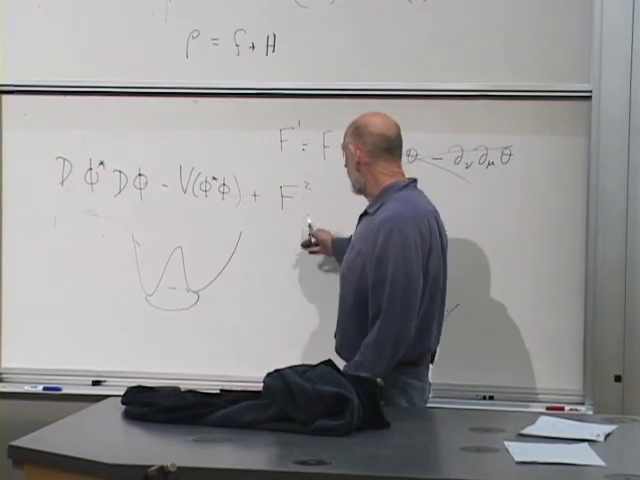
\includegraphics[width=0.76\textwidth]{lecture_08_figure_05.png}
\caption{經確認的黑板內容呈現了這項障礙：在規範變換下，\(A_\mu A^\mu\) 會變成一個包含 \(\partial_\mu\theta\) 的平方項，因此裸向量質量項並非不變量。}
\lectureframe{01:07:30}
\label{fig:l08-bare-mass-board}
\end{figure}

\section{希格斯機制}

\subsection{協變導數如何產生質量}

回到對稱性破缺的勢能，採用正則歸一化的參數表示
\begin{equation}
  \phi(x)=\frac{f+h(x)}{\sqrt2}
  e^{i\pi(x)/f}.
\end{equation}
其協變導數為
\begin{equation}
  D_\mu\phi
  =
  \frac{e^{i\pi/f}}{\sqrt2}
  \left[
    \partial_\mu h
    +i(f+h)
      \left(\frac{\partial_\mu\pi}{f}+gA_\mu\right)
  \right].
  \label{eq:l08-covariant-polar}
\end{equation}
因此，
\begin{equation}
\begin{aligned}
  (D_\mu\phi)^*D^\mu\phi
  ={}&
  \frac12(\partial_\mu h)^2
  \\
  &+\frac12(f+h)^2
    \left(\frac{\partial_\mu\pi}{f}+gA_\mu\right)
  \\
  &\hspace{4.2em}\times
    \left(\frac{\partial^\mu\pi}{f}+gA^\mu\right).
\end{aligned}
  \label{eq:l08-higgs-kinetic}
\end{equation}

關鍵項在作任何規範選擇之前就已出現：
\begin{equation}
  \frac12g^2f^2 A_\mu A^\mu.
  \label{eq:l08-vector-mass-term}
\end{equation}
與普羅卡形式 \(\frac12m_A^2A_\mu A^\mu\) 比較，可得
\begin{equation}
  \boxed{m_A=g f}.
  \label{eq:l08-vector-mass}
\end{equation}
同一次展開也會產生交互作用項 \(g^2fh A_\mu A^\mu\) 和 \(\frac12g^2h^2A_\mu A^\mu\)。因此，向量質量並非任意破壞規範對稱性的結果，而是從規範不變的純量動能項產生；此項是在平衡幅值 \(f\) 不為零的相中計算。

\begin{figure}[htbp]
\centering
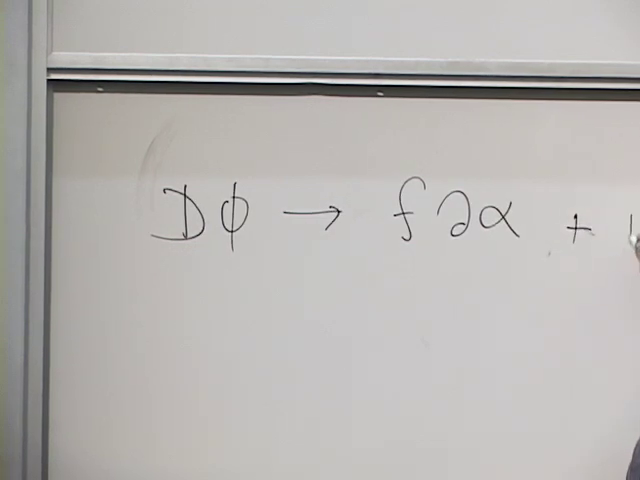
\includegraphics[width=0.78\textwidth]{lecture_08_figure_06.png}
\caption{黑板從 \((D\phi)^*(D\phi)\) 中分離出 \(f^2A^2\) 項。在式 ~\eqref{eq:l08-canonical-polar} 和 \eqref{eq:l08-covariant-convention} 所採用的歸一化下，結果為 \(m_A=gf\)；數值因子會依純量場和規範耦合常數的歸一化方式而異。}
\lectureframe{01:10:10}
\label{fig:l08-generated-mass-board}
\end{figure}

講座將 \(g\) 和數個 \(\sqrt2\) 因子吸收到黑板記號中，因此在標示質量時，短暫地交替使用 \(f\)、\(2f\) 和 \(\sqrt2f\)。除非先說明動能項和勢能的歸一化方式，否則這些因子並沒有不依賴約定的意義。穩健的結果是 \(m_A\propto gf\)；式 ~\eqref{eq:l08-vector-mass} 給出了此處採用的約定所對應的因子。

\subsection{吸收相位}

在規範變換下，相位變數的變化為
\begin{equation}
  \pi'(x)=\pi(x)+f\,\theta(x).
\end{equation}
選擇
\begin{equation}
  \theta(x)=-\frac{\pi(x)}{f}.
  \label{eq:l08-unitary-gauge-choice}
\end{equation}
便有 \(\pi'=0\)。這就是么正規範；在此規範下，\begin{equation}
  \phi'(x)=\frac{f+h(x)}{\sqrt2}
\end{equation} 為實數，而式 ~\eqref{eq:l08-higgs-kinetic} 化為
\begin{equation}
  (D_\mu\phi')^*D^\mu\phi'
  =
  \frac12(\partial_\mu h)^2
  +\frac12g^2(f+h)^2A_\mu'A^{\prime\mu}.
  \label{eq:l08-unitary-gauge-lagrangian}
\end{equation}
角向戈德斯通場不再是獨立變數，但向量質量仍然存在。

講座先在低能極限 \(\rho=f\) 下展示這一點，此時
\begin{align}
  \phi&=f e^{i\alpha},
  \notag\\
  D_\mu\phi
  &=if e^{i\alpha}
    \left(\partial_\mu\alpha+gA_\mu\right),
  \notag\\
  (D_\mu\phi)^*
  &=-if e^{-i\alpha}
    \left(\partial_\mu\alpha+gA_\mu\right).
  \label{eq:l08-frozen-radius}
\end{align}
兩者相乘得到
\begin{equation}
  f^2
  \left(\partial_\mu\alpha+gA_\mu\right)
  \left(\partial^\mu\alpha+gA^\mu\right).
\end{equation}
選擇 \(\theta=-\alpha\) 後，便剩下 \(g^2f^2A_\mu'A^{\prime\mu}\)。

\begin{figure}[htbp]
\centering
\includegraphics[width=0.82\textwidth]{lecture_08_figure_07.png}
\caption{固定半徑下的完整板書狀態：協變導數同時包含相位導數與向量位勢。接著，講座中選取\(\theta=-\alpha\)以消去相位，留下向量質量項。}
\lectureframe{01:16:20}
\label{fig:l08-frozen-radius-board}
\end{figure}

\begin{classroomqa}
\audiencequestion{能否改用一組變數重寫整個拉格朗日量，讓角向模態如何消失一目了然？
\lecturetimestamp{01:13:49}}
\lecturerresponse{可以。在極座標變數中，相位只會透過規範不變的組合 \(\partial_\mu\alpha+gA_\mu\) 出現。作規範變換並取 \(\theta=-\alpha\)，就能在此規範定義良好的所有位置將相位設為零。如此一來，純量動能項便成為向量質量項，而規範不變的場強項維持不變。}
\end{classroomqa}

\begin{classroomqa}
\audiencequestion{\(\alpha\)中的振盪，和規範振盪無法區分嗎？\lecturetimestamp{01:18:02}}
\lecturerresponse{在規範化理論中，若 \(\alpha\) 的純粹變化由 \(A_\mu\) 的相應變化抵銷，那只是對規範的重新描述，不代表另一個物理波。規範不變的量是 \(\partial_\mu\alpha+gA_\mu\)。原先由全域戈德斯通場描述的物理模態，則成為有質量向量的縱向偏振。}
\end{classroomqa}

常有人說局域規範對稱性會自發破缺。就實際操作而言，這種說法很有用：選定規範後，純量場具有非零真空值，粒子譜中也會出現有質量的向量。不過嚴格來說，規範變換關聯的是冗餘描述，而非不同的物理態。
\editorialnote{局域規範冗餘並不像全域對稱性那樣，以規範不變的意義破缺。更精確地說，該理論處於希格斯相。固定規範後的微擾論，則以非零的純量期望值及由此產生的有質量向量粒子譜來描述這個相。}

\section{戈德斯通自由度去了哪裡}

改變變數不會讓任何物理自由度憑空消失。來比較進入希格斯相前後的自由度數目。

之前：
\begin{equation}
  \underbrace{2}_{\text{massless vector}}
  +
  \underbrace{2}_{\text{complex scalar}}
  =4.
\end{equation}
無質量向量有兩個橫向偏振；複純量則有兩個實分量，分別是徑向和角向分量。

之後：
\begin{equation}
  \underbrace{3}_{\text{massive vector}}
  +
  \underbrace{1}_{\text{radial Higgs}}
  =4.
  \label{eq:l08-degree-count}
\end{equation}
有質量的向量可以在其靜止系中描述。靜止系裡沒有任何空間方向特別突出，因此它必須有三種偏振態。向量運動時，其中兩種是橫向偏振，一種是縱向偏振。戈德斯通模態便成為這個縱向偏振。

\begin{figure}[htbp]
\centering
\begin{adjustbox}{max width=\linewidth}
\begin{tikzpicture}[x=1cm,y=1cm]
  \node[draw,rounded corners,fill=blue!7,minimum width=4.3cm,
        minimum height=2.1cm,align=center] (before) at (0,0)
    {massless \(A_\mu\): \(2\) transverse\\
     \(+\)\\
     complex \(\phi\): \(h+\pi\)};
  \node[draw,rounded corners,fill=orange!10,minimum width=4.3cm,
        minimum height=2.1cm,align=center] (after) at (7,0)
    {massive \(A_\mu\): \(2\) transverse\\
     \(+\;1\) longitudinal\\
     \(+\) radial \(h\)};
  \draw[->,very thick] (before) -- node[above]{Higgs phase} (after);
  \draw[->,teal!70!black,thick]
    (-0.15,-0.65) to[bend right=28]
    node[below,align=center]{Goldstone \(\pi\) supplies\\longitudinal mode}
    (6.8,-0.65);
\end{tikzpicture}
\end{adjustbox}
\caption{希格斯機制重組了物理自由度，並未消滅它們。}
\label{fig:l08-degree-rearrangement}
\end{figure}

\begin{classroomqa}
\audiencequestion{角向自由度如何在不違反自由度計數的情況下消失？\lecturetimestamp{01:19:13}}
\lecturerresponse{它在物理上並沒有消失。無質量向量不能靜止，因此只有兩種螺旋度；有質量向量則有三種偏振，包括一種縱向偏振。戈德斯通模態成為第三種偏振，因此總自由度數目維持不變。}
\end{classroomqa}

講座提供了一個實用的運動學檢驗。設想一個有質量的向量粒子：先讓它減速至靜止，再沿新的方向加速。原本相對於舊運動方向為橫向的偏振，相對於新的運動方向可能變成縱向。同樣地，如果一個圓偏振的有質量粒子經過靜止，再沿相反方向運動，它的螺旋度標記就會反轉。嚴格無質量的粒子無法經歷這項實驗，因為任何慣性參考系都不能讓它靜止。因此，無質量粒子的兩種螺旋度構成一致的物理譜。

\section{超導體的類比}

在傳統超導體中，電子會形成庫珀對。每個庫珀對都是攜帶電荷 \(2e\) 的玻色子，而凝聚態則以帶電的複數序參量描述。當序參量的幅值不為零時，其相位與電磁向量勢結合，便產生安德森--希格斯機制。靜磁場會在倫敦穿透深度範圍內衰減，而不會自由延伸至超導體內部。就這個明確且依介質而定的意義而言，光子表現得彷彿獲得了質量。

這個例子也釐清了開頭提到的區別。電磁場並未永久轉變成另一種基本粒子。有質量的傳播定律適用於材料內部的集體態；在材料外部，真空中的光子仍是無質量的。

\section{目前得到的結論}

現在可以在不失去論證脈絡的前提下，將內容簡要整理如下：
\begin{enumerate}
  \item 全域連續對稱性破缺後，角向有一個平坦方向，因此會有無質量的戈德斯通模態。
  \item 局域相位不變性要求引入規範勢，並以 \(D_\mu\) 取代 \(\partial_\mu\)。
  \item 裸的 \(A_\mu A^\mu\) 質量違反局域變換律。
  \item 帶電純量的平衡幅值 \(f\) 不為零時，規範不變項 \(|D_\mu\phi|^2\) 會包含 \(\frac12g^2f^2A_\mu A^\mu\)。
  \item 選擇規範即可消去相位；相位所對應的物理自由度，會成為有質量向量的縱向偏振。
  \item 徑向希格斯激發仍然存在，其質量由純量勢能的曲率決定。
\end{enumerate}

接下來要說明費米子如何獲得質量。電子和夸克不能直接採用向量機制；它們透過湯川交互作用與希格斯場耦合。純量場穩定在 \(f\) 後，這些交互作用便成為費米子質量項。

「若沒有電弱對稱性破缺，我們熟悉的粒子都沒有質量」這個概括性的說法，還需要再加上一項限定。基本夸克和帶電輕子的質量，以及 \(W\) 和 \(Z\) 的質量，確實會隨希格斯期望值消失。然而，質子和中子的大部分質量來自 QCD 禁閉和強場能量的動力學效應，而非夸克的希格斯質量。這項區別不會改變此處推導的希格斯機制，只是讓我們更精確地界定它的適用範圍。

\chapter{費米子質量：手徵性、湯川耦合與馬約拉納中微子}

\lectureoverview{我們先在玩具\(U(1)\)理論中重新推導規範玻色子的希格斯機制，再對費米子提出相應的問題。狄拉克質量會混合左、右手徵場，但弱相互作用賦予兩者不同的荷，因此禁止裸質量。與希格斯場的湯川耦合符合對稱性；希格斯場取得真空值後，同一個相互作用便成為費米子質量，以及可測量的希格斯--費米子耦合。最後一部分將沿著這個脈絡，探討中微子質量、可能存在的未受保護重粒子、宇宙射線運動學、相對論中的慣性，以及重力。}

開場回顧的目的不只是重述上一講的內容。我們需要從中提取一個可延伸至費米子的觀念：質量是零動量激發態所具有的非零能量。對場而言，零動量意味著無限波長，也就是處處相同的位移。只有導數項的理論無法感知均勻位移；不含導數的項則可以。

\section{規範玻色子的機制：快速回顧}

\subsection{導數能量與無質量向量場}

模型中的規範場是\(A_\mu\)，其場強為
\begin{equation}
  F_{\mu\nu}
  =\partial_\mu A_\nu-\partial_\nu A_\mu .
  \label{eq:l09-field-strength}
\end{equation}
黑板上以示意方式將規範場的動能項寫成\(F^2\)。採用標準歸一化後，它的形式為
\begin{equation}
  \mathcal L_{\mathrm{gauge}}
  =-\frac14 F_{\mu\nu}F^{\mu\nu}.
  \label{eq:l09-gauge-kinetic}
\end{equation}

\begin{figure}[htbp]
\centering
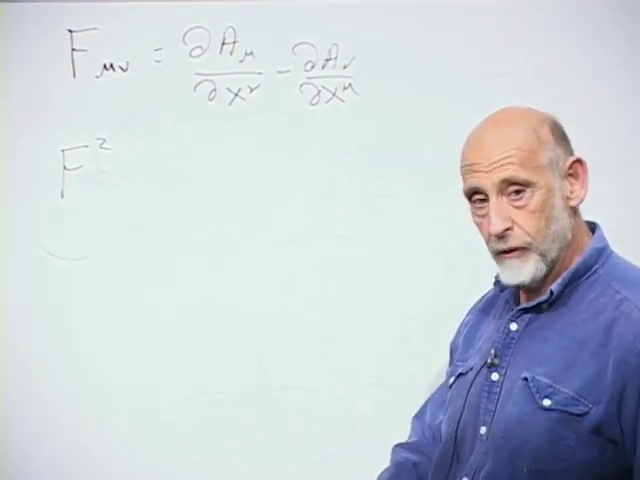
\includegraphics[width=0.72\textwidth]{lecture_09_figure_02.png}
\caption{場強的定義，以及黑板上以\(F^2\)表示規範場導數能量的簡寫。}
\lectureframe{00:02:39}
\label{fig:l09-field-strength-board}
\end{figure}

在\eqref{eq:l09-gauge-kinetic}中，每一個\(A_\mu\)都經過微分。因此，
\begin{equation}
  A_\mu(x)\longmapsto A_\mu(x)+c_\mu,
  \qquad \partial_\nu c_\mu=0,
\end{equation}
不會改變\(F_{\mu\nu}\)。所以，均勻的向量勢不會產生場強能量。用本講的說法，零動量模沒有能隙，規範玻色子因此是無質量的。

這個\(U(1)\)場是刻意簡化的替代模型。實際要討論的是\(W^\pm\)和\(Z\)，而非電磁光子。未破缺的電磁對稱性使光子保持無質量；電弱對稱性的破缺則使弱規範玻色子取得質量。

\subsection{凍結希格斯場的徑向自由度}

引入一個帶電複純量場，並將它寫成極座標形式：
\begin{equation}
  \phi(x)=\rho(x)e^{i\alpha(x)}.
\end{equation}
它的墨西哥帽勢在半徑非零的圓周上取極小值。將這個半徑記為\(f\)；徑向方向的變化相對而言代價較高。第一步先凍結徑向自由度，只保留相位：
\begin{equation}
  \phi(x)\simeq f e^{i\alpha(x)}.
  \label{eq:l09-frozen-higgs}
\end{equation}

\begin{figure}[htbp]
\centering
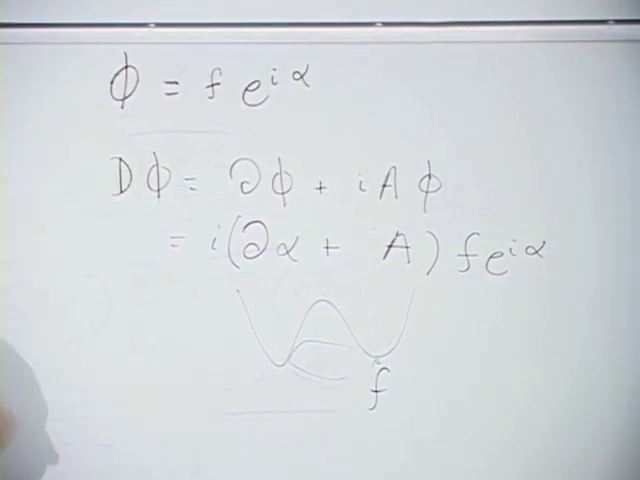
\includegraphics[width=0.72\textwidth]{lecture_09_figure_03.png}
\caption{凍結的希格斯場徑向自由度、其協變導數，以及回顧時使用的簡化破缺勢示意圖。}
\lectureframe{00:06:42}
\label{fig:l09-frozen-board}
\end{figure}

採用以下約定：
\begin{equation}
\begin{aligned}
  D_\mu&=\partial_\mu+igA_\mu,
  \\
  \phi&\longmapsto e^{i\theta}\phi,
  \\
  A_\mu&\longmapsto A_\mu-\frac1g\partial_\mu\theta .
\end{aligned}
  \label{eq:l09-gauge-convention}
\end{equation}
本講省略了\(g\)；將它明確寫出，量綱和最後得到的質量便一目了然。協變導數作用在凍結的場上，得到
\begin{align}
  D_\mu\phi
  &=(\partial_\mu+igA_\mu)f e^{i\alpha}
  \notag\\
  &=i\bigl(\partial_\mu\alpha+gA_\mu\bigr)
    f e^{i\alpha}.
  \label{eq:l09-covariant-frozen}
\end{align}
乘上複共軛後，相位會消去，而\(i\)與\(-i\)相乘也會得到\(+1\)：
\begin{equation}
  |D_\mu\phi|^2
  =f^2
   \bigl(\partial_\mu\alpha+gA_\mu\bigr)
   \bigl(\partial^\mu\alpha+gA^\mu\bigr).
  \label{eq:l09-frozen-square}
\end{equation}

\begin{classroomqa}
\audiencequestion{協變導數的平方是否應該帶負號？畢竟微分後會出現\(i\)因子。
\lecturetimestamp{00:07:39}}
\lecturerresponse{不需要。動能項是協變導數與其複共軛的乘積。一個因子帶來\(i\)，另一個帶來\(-i\)，而\(i(-i)=1\)。\(D_\mu\)的符號約定可以一致地反轉，但相應能量表達式中的模平方仍為正。}
\end{classroomqa}

\eqref{eq:l09-frozen-square}中的組合本身就是經過位移的規範場。選擇\(\theta=-\alpha\)，使純量場的相位消去，並定義
\begin{equation}
  A'_\mu=A_\mu+\frac1g\partial_\mu\alpha .
  \label{eq:l09-unitary-gauge-field}
\end{equation}
於是
\begin{equation}
  |D_\mu\phi|^2=g^2f^2 A'_\mu A'^\mu .
  \label{eq:l09-vector-mass-term}
\end{equation}
新項不含\(A'_\mu\)的導數。均勻場現在具有能量，因此零動量向量模出現能隙。

\begin{figure}[htbp]
\centering
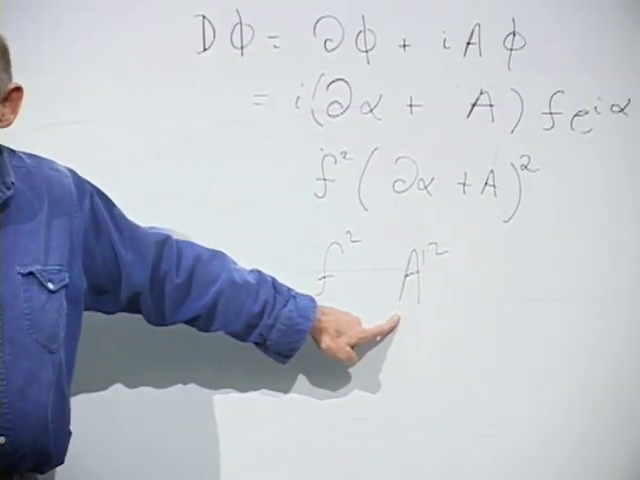
\includegraphics[width=0.72\textwidth]{lecture_09_figure_04.png}
\caption{黑板上單獨列出\(f^2A^2\)項；相位吸收後，這一項標示出規範玻色子質量的產生。}
\lectureframe{00:10:31}
\label{fig:l09-vector-mass-board}
\end{figure}

採用正則純量場歸一化時，可寫成
\(\phi=(f+h)e^{i\pi/f}/\sqrt2\)。將得到的向量場項與
\(\tfrac12m_A^2A_\mu A^\mu\)相比，可得
\begin{equation}
  m_A=gf
  \label{eq:l09-abelian-vector-mass}
\end{equation}
這就是此阿貝爾模型中的結果。本講略去歸一化因子，並以向量場質量由\(f\)決定來概括。

相位模並非無故消失。在規範化之前，它是無質量的戈德斯通玻色子；規範化之後，它提供了有質量向量粒子所需的縱向偏振自由度。我們暫時凍結的徑向漲落，則保留為物理希格斯激發。

\subsection{為什麼不含導數的項代表質量}

\begin{classroomqa}
\audiencequestion{為什麼\(A'^2\)項代表質量，而不只是另一種相互作用？\lecturetimestamp{00:13:10}}
\lecturerresponse{質量就是靜止能量。對場而言，靜止粒子是零動量、無限波長模態的量子。導數項不會讓靜止的均勻位移具有能量，但\(m_A^2A'^2\)會。這個零動量時仍存在的非零能量，就是靜止能量的能隙。}
\end{classroomqa}

本講透過三個力學類比來說明這一點。

\begin{itemize}
  \item 在晶體中，緩慢變化的位移會產生彈性能，因為相鄰原子的位移不同。若所有原子一起剛性平移，則不會產生內能。因此，聲學聲子沒有能隙。
  \item 在理想的旋轉對稱磁體中，空間變化的自旋方向會產生交換能；若所有自旋一起旋轉，則不會。相應的長波長自旋波沒有能隙。
  \item 在電漿中，電子流體相對於正電荷背景發生位移會造成電荷分離，並產生恢復電場；即使相對位移是均勻的，情況也是如此。因此，等離激元在零波數時仍具有非零頻率。
\end{itemize}

希格斯機制下的規範場表現得像第三個例子：破缺後的介質會抵抗原本不需付出能量的均勻位移。

\begin{classroomqa}
\audiencequestion{引入規範場之前，相位\(\alpha\)不是已經會振動了嗎？\lecturetimestamp{00:18:24}}
\lecturerresponse{會。它的能量正比於\(f^2(\partial_\mu\alpha)^2\)。相位若隨位置變化，便具有梯度能量，也能傳播；但均勻改變相位不需付出能量。這正是無質量的戈德斯通模態。}
\end{classroomqa}

\begin{classroomqa}
\audiencequestion{導數中也包含時間導數。若真的移動整個晶格，或改變整個場，難道不會帶有動能嗎？\lecturetimestamp{00:22:18}}
\lecturerresponse{會。這裡比較的是靜態構型，或以任意緩慢的方式準備出的構型。晶格若以非零速度平移，就具有動能。判斷質量時要問的是：構型處於靜止且空間均勻時，是否仍具有能量。}
\end{classroomqa}

\section{實驗線索：弱相互作用區分左右}

接著轉向電子、{\proseunicodefont μ}子和夸克。它們的質量也來自希格斯場，但機制看起來不同，因為費米子質量不是向量場的二次項，而是兩個手徵場之間的耦合。

\subsection{{\proseunicodefont β} 衰變中的宇稱破壞}

先從弱相互作用會破壞宇稱這項實驗事實談起。量子電動力學和量子色動力學對某個過程及其鏡像過程一視同仁；弱相互作用則不然。在中子 {\proseunicodefont β} 衰變中，
\begin{equation}
  n\longrightarrow p+e^-+\bar\nu_e,
  \label{eq:l09-beta-decay}
\end{equation}
帶電流相互作用所選出的高能電子具有左手螺旋度：它們的自旋方向與動量方向相反。相應的反中微子則具有相反的螺旋度。

對超相對論粒子，螺旋度定義為
\begin{equation}
  h=\frac{\bm S\cdot\bm p}{|\bm S|\,|\bm p|}.
\end{equation}
自旋平行於動量時，螺旋度為\(h=+1\)；自旋反平行於動量時，則為\(h=-1\)。
弱相互作用會耦合到左手徵電子場與左手徵中微子場，但不會以相同方式耦合到右手徵電子場。\editorialnote{本講一開始用螺旋度來談左右手性，因為在高能下這種說法直觀易懂。但規範荷實際作用於手徵性，也就是由\(P_L=(1-\gamma^5)/2\)和\(P_R=(1+\gamma^5)/2\)選定的洛侖茲表示標籤。對無質量粒子而言，粒子的手徵性與螺旋度一致；對有質量粒子而言，兩者則不相同。}

為了不必處理完整的\(SU(2)_L\times U(1)_Y\)記號，就能看出這個障礙，可以設想一個虛構的\(U(1)\)世界，其中只有\(\psi_L\)帶有相關的荷：
\begin{equation}
  \psi_L\longmapsto e^{i\theta}\psi_L,
  \qquad
  \psi_R\longmapsto\psi_R .
  \label{eq:l09-chiral-toy-charge}
\end{equation}
這不是電磁學；真實的左、右手徵電子帶有相同的電荷。這只是弱相互作用的簡化圖像：兩種手徵性屬於不同的電弱表示。

\begin{classroomqa}
\audiencequestion{夸克也有相同的左--右不對稱性嗎？\lecturetimestamp{00:31:50}}
\lecturerresponse{有，但須考慮適當的弱多重態和超荷。左手徵的上型與下型夸克組成弱二重態，右手徵場則是弱單態。因此，它們的希格斯耦合同樣面臨與電子相同的結構性問題。}
\end{classroomqa}

\section{狄拉克質量會混合左--右}

\subsection{從四分量方程到兩個韋爾方程}

狄拉克波函數有四個分量。粗略而言，其中兩個描述自旋，另外兩個區分正能量解與負能量解；後者重新詮釋為反粒子的自由度。寫成哈密頓形式：
\begin{equation}
  i\frac{\partial\Psi}{\partial t}
  =\left(-i\bm\alpha\cdot\bm\nabla+m\beta\right)\Psi .
  \label{eq:l09-dirac-hamiltonian}
\end{equation}
矩陣\(\alpha_i\)和\(\beta\)表現了能量、動量與質量之間的相對論關係。

\begin{figure}[htbp]
\centering
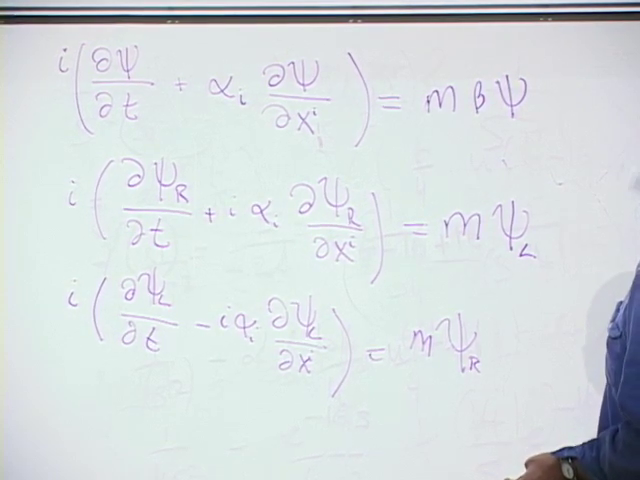
\includegraphics[width=0.74\textwidth]{lecture_09_figure_05.png}
\caption{黑板上先寫出狄拉克方程，再將它拆解為彼此耦合的左、右手徵方程。}
\lectureframe{00:40:30}
\label{fig:l09-dirac-board}
\end{figure}

手徵基底明確呈現了\(m\)的作用。令
\(\sigma^\mu=(1,\bm\sigma)\)和
\(\bar\sigma^\mu=(1,-\bm\sigma)\)，則
\begin{align}
  i\bar\sigma^\mu\partial_\mu\psi_L&=m\psi_R,
  \label{eq:l09-weyl-left}\\
  i\sigma^\mu\partial_\mu\psi_R&=m\psi_L.
  \label{eq:l09-weyl-right}
\end{align}
當\(m=0\)時，兩個方程彼此獨立：左手徵場和右手徵場可以各自傳播，互不耦合。當\(m\neq0\)時，每個場都成為另一個場的源。這就是狄拉克質量混合左右手徵場的確切含義。

Susskind將此描述為費米子在左右手徵之間振盪。這種說法點出了耦合，但不應將它延伸成點粒子來回翻轉的字面圖像。精確的說法是，場方程彼此耦合：
\eqref{eq:l09-weyl-left}--\eqref{eq:l09-weyl-right}。

\begin{classroomqa}
\audiencequestion{黑板上兩個方程中的\(i\)因子和符號是否一致？\lecturetimestamp{00:41:10}}
\lecturerresponse{黑板上的寫法並非逐行一致；快速推導時，有一個\(i\)被不一致地提出方程之外。可靠的內容是耦合的形式。方程\eqref{eq:l09-weyl-left}和
\eqref{eq:l09-weyl-right}給出一套標準且一致的約定。}
\end{classroomqa}

\subsection{為什麼弱對稱性禁止裸質量}

相應的狄拉克質量項在拉格朗日量中寫為
\begin{equation}
  \mathcal L_m
  =-m\bar\psi\psi
  =-m\left(\bar\psi_L\psi_R+\bar\psi_R\psi_L\right).
  \label{eq:l09-bare-dirac-mass}
\end{equation}
在玩具模型的變換\eqref{eq:l09-chiral-toy-charge}下，
\begin{equation}
  \bar\psi_L\psi_R\longmapsto
  e^{-i\theta}\bar\psi_L\psi_R,
  \qquad
  \bar\psi_R\psi_L\longmapsto
  e^{i\theta}\bar\psi_R\psi_L.
\end{equation}
兩項都不是不變量。因此，在對稱性破缺之前，直接混合左--右手徵場的係數\(m\)會受到禁止。

單靠電磁作用不會造成這個問題，因為\(\psi_L\)和\(\psi_R\)具有相同的電荷。這個障礙源自兩者不同的弱量子數。

\subsection{揭示手徵性微妙之處的螺旋度問題}

接著，課堂從幾個角度檢驗直觀的左右手性圖像。這些問題並非枝節；它們正好揭示螺旋度在哪些情況下有用，又在哪些情況下必須改以手徵性來描述。

\begin{classroomqa}
\audiencequestion{如果弱相互作用以相同的機率產生兩種螺旋度的電子，世界會是什麼樣子？\lecturetimestamp{00:42:12}}
\lecturerresponse{該過程中的宇稱不對稱性會立即消失。但真實的電弱理論具有手徵性：只有左手徵二重態帶有帶電流弱相互作用。至於自然界為何採取這種結構，本講將延後再作更完整的說明。}
\end{classroomqa}

\begin{classroomqa}
\audiencequestion{假設電子的自旋沿垂直方向準備，接著電子沿水平方向加速。它是左手性還是右手性？\lecturetimestamp{00:42:44}}
\lecturerresponse{自旋若垂直於動量方向，該自旋態就是兩種螺旋度的疊加。只有當自旋平行或反平行於動量時，螺旋度才有確定值。不過，對場而言，弱手徵投影算符仍有明確定義。}
\end{classroomqa}

有質量粒子可以減速至靜止，再沿相反方向加速，而自旋方向保持不變。此時它的螺旋度會改變符號。無質量粒子無法被洛侖茲推進追上或帶至靜止，因此其螺旋度在固有推進下保持不變。這是本講所說「只有一種物理螺旋度的粒子種類必須無質量」的理由。更精確的場論說法是，洛侖茲不變的狄拉克質量需要兩種手徵性。

\begin{classroomqa}
\audiencequestion{圓偏振光子可以從鏡面反射，改變傳播方向，卻從未靜止。這是否與螺旋度論證矛盾？\lecturetimestamp{00:45:28}}
\lecturerresponse{不矛盾。鏡子是外部系統，可以交換角動量並反轉傳播方向。反射過程並不是透過洛侖茲推進追上光子。某個通道是否存在，也取決於允許的偏振態和材料的邊界條件。}
\end{classroomqa}

\begin{classroomqa}
\audiencequestion{一般的電子束具有一種手性，還是兩種都有？\lecturetimestamp{00:46:10}}
\lecturerresponse{一般而言，兩種都有。有質量電子態包含兩種手徵分量，而未偏振的電子束包含兩種螺旋度。專用的電子源則可以產生螺旋度不對稱性很大的偏振束。}
\end{classroomqa}

\begin{classroomqa}
\audiencequestion{束流能否在不受自旋影響的情況下聚焦？還是磁場會將兩種偏振分開？\lecturetimestamp{00:46:29}}
\lecturerresponse{一般的位置聚焦大致上可以不受自旋影響，但磁矩會與磁場梯度耦合。因此，自旋選擇性電子源、類似斯特恩--格拉赫實驗的磁場梯度，以及加速器中的自旋動力學，都可以用來製備或分離不同偏振態。}
\end{classroomqa}

\begin{classroomqa}
\audiencequestion{弱相互作用對左右的差異只是偶然嗎？\lecturetimestamp{00:48:13}}
\lecturerresponse{就本課程而言，這是納入標準模型的實驗事實。其規律性如此強，不像隨意的偶然；但標準模型本身並未從更深層的原理推導出完整的手徵荷排列。}
\end{classroomqa}

\section{湯川耦合的建構}

\subsection{讓希格斯場帶有缺少的荷}

對稱性禁止直接加入數值質量，卻允許與某個場相互作用，由該場提供缺少的變換相位。引入一個複純量場，使其滿足
\begin{equation}
  \phi\longmapsto e^{i\theta}\phi,
  \qquad
  \phi^\dagger\longmapsto e^{-i\theta}\phi^\dagger.
  \label{eq:l09-scalar-charge}
\end{equation}
則
\begin{equation}
  \mathcal L_Y
  =-y\,\bar\psi_L\phi\psi_R
   -y^*\,\bar\psi_R\phi^\dagger\psi_L
  \label{eq:l09-yukawa-lagrangian}
\end{equation}
便具有規範不變性。在第一項中，
\(\bar\psi_L\)帶來\(e^{-i\theta}\)，而\(\phi\)帶來\(e^{i\theta}\)；兩個相位彼此抵消。第二項是其厄米共軛。

等價地，手徵方程中會出現依賴場的混合項：
\begin{align}
  i\bar\sigma^\mu D_\mu\psi_L
    &=y\phi\psi_R,
  \label{eq:l09-yukawa-eom-left}\\
  i\sigma^\mu\partial_\mu\psi_R
    &=y^*\phi^\dagger\psi_L.
  \label{eq:l09-yukawa-eom-right}
\end{align}

\begin{figure}[htbp]
\centering
\includegraphics[width=0.76\textwidth]{lecture_09_figure_06.png}
\caption{方程右側的裸質量已由帶電純量場取代。黑板上的具體符號僅為示意；不變的結構見\eqref{eq:l09-yukawa-lagrangian}。}
\lectureframe{00:51:30}
\label{fig:l09-yukawa-board}
\end{figure}

對稱性破缺之前，這是一種相互作用，而非質量。右手徵費米子只有在發射或吸收用來平衡荷的純量量子時，才能轉變為左手徵費米子。係數\(y\)是湯川耦合，不是規範荷\(g\)。

\begin{classroomqa}
\audiencequestion{直接將\(\phi\)和\(\phi^\dagger\)放在兩個方程右側，這樣合理嗎？
\lecturetimestamp{00:51:55}}
\lecturerresponse{合理，正是因為它們的變換相位補上了不匹配之處。關鍵不在方程表面上的形式，而在於相互作用\(\bar\psi_L\phi\psi_R+\mathrm{h.c.}\)是否具有規範不變性。}
\end{classroomqa}

\subsection{真空將相互作用轉化為質量}

現在將\(\phi\)視為希格斯場，並讓它穩定在非零的真空幅值。在本講採用的簡化歸一化下，
\begin{equation}
  \phi\simeq f,
\end{equation}
因此\eqref{eq:l09-yukawa-lagrangian}包含
\begin{equation}
  \mathcal L_Y
  \supset
  -yf\,\bar\psi_L\psi_R
  -y^*f\,\bar\psi_R\psi_L .
\end{equation}
在適當的情況下，經過不影響物理的相位重新定義後，費米子質量為
\begin{equation}
  m_f=yf.
  \label{eq:l09-lecture-fermion-mass}
\end{equation}
這是向量場結果\(m_A=gf\)在費米子上的對應。為弱規範玻色子提供縱向偏振自由度的同一個希格斯真空，也提供了連結左、右手徵費米子所需的弱量子數。

採用標準模型的正則歸一化慣例時，
\begin{equation}
  H(x)=\frac1{\sqrt2}
  \begin{pmatrix}
    0\\ v+h(x)
  \end{pmatrix},
  \qquad v\simeq246\ \mathrm{GeV},
  \label{eq:l09-sm-higgs-vacuum}
\end{equation}
因此
\begin{equation}
  m_f=\frac{y_fv}{\sqrt2}.
  \label{eq:l09-sm-fermion-mass}
\end{equation}
本講採用的\(f\)與慣用的\(v/\sqrt2\)僅在歸一化選擇上有所不同。

\begin{classroomqa}
\audiencequestion{如果只有乘積\(yf\)才是費米子質量，如何分別求出耦合\(y\)與真空尺度\(f\)？
\lecturetimestamp{00:55:36}}
\lecturerresponse{已知規範耦合後，弱規範玻色子的質量可以決定真空尺度；再由費米子的測得質量決定其湯川耦合。在完整理論中，
\(m_W=gv/2\)、\(m_Z=v\sqrt{g^2+g'^2}/2\)和\(y_f=\sqrt2m_f/v\)。}
\end{classroomqa}

\begin{classroomqa}
\audiencequestion{弱玻色子的質量大約是\(900\ \mathrm{GeV}\)嗎？\lecturetimestamp{00:57:43}}
\lecturerresponse{不是；講座隨即更正口誤，指出大約是\(90\ \mathrm{GeV}\)。更精確地說，
\(m_W\simeq80\ \mathrm{GeV}\)和\(m_Z\simeq91\ \mathrm{GeV}\)，而真空的基本尺度為\(v\simeq246\ \mathrm{GeV}\)。}
\end{classroomqa}

\subsection{一個真空尺度，多種湯川耦合}

每一種帶電費米子都有各自的湯川耦合：
\begin{equation}
  m_i=y_i f
  \qquad\text{(lecture normalization)}.
  \label{eq:l09-mass-family}
\end{equation}

\begin{figure}[htbp]
\centering
\includegraphics[width=0.76\textwidth]{lecture_09_figure_08.png}
\caption{黑板以\(m_i=g_i f\)概括不同粒子的差異；其中的\(g_i\)就是此處所稱的湯川耦合\(y_i\)。}
\lectureframe{01:16:30}
\label{fig:l09-mass-family-board}
\end{figure}

本講估算電子的湯川耦合為
\begin{equation}
  y_e\sim\frac{0.5\ \mathrm{MeV}}{10^2\ \mathrm{GeV}}
  \sim10^{-5}.
\end{equation}
使用正則歸一化的數值\(v=246\ \mathrm{GeV}\)後，可得更精確的結果：
\(y_e\simeq2.9\times10^{-6}\)。頂夸克則位於另一個極端：
\begin{equation}
  y_t=\frac{\sqrt2m_t}{v}\simeq1.
\end{equation}
因此，希格斯機制解釋了規範不變的質量如何存在，卻沒有解釋各個\(y_i\)之間為何有如此巨大的階層差異。觀測到的費米子質量只是把這種差異呈現為測量數值。

\begin{classroomqa}
\audiencequestion{頂夸克的湯川耦合真的約為一嗎？\lecturetimestamp{00:59:09}}
\lecturerresponse{是的。頂夸克的質量與電弱尺度相當，因此其耦合不像電子的耦合那樣微小。在現代的歸一化慣例下，\(y_t\)接近一。}
\end{classroomqa}

\subsection{恢復物理的希格斯場漲落}

將純量場凍結在真空值，會把徑向激發隱藏起來。現在以示意方式將它恢復：
\begin{equation}
  \phi(x)\simeq f+h(x).
\end{equation}
湯川因子便成為
\begin{equation}
  y\phi\simeq yf+yh=m_f+yh.
  \label{eq:l09-mass-plus-higgs}
\end{equation}

\begin{figure}[htbp]
\centering
\includegraphics[width=0.76\textwidth]{lecture_09_figure_07.png}
\caption{黑板上的湯川項恢復了希格斯場漲落：常數部分產生費米子質量，漲落部分則讓希格斯玻色子得以發射或吸收。}
\lectureframe{01:01:15}
\label{fig:l09-higgs-fluctuation-board}
\end{figure}

\eqref{eq:l09-mass-plus-higgs}中的第一項是質量項。第二項則是希格斯玻色子與費米子耦合的頂點。採用標準模型的慣用記法時，
\begin{equation}
  \mathcal L_Y
  \supset
  -m_f\bar\psi\psi
  -\frac{m_f}{v}h\bar\psi\psi.
  \label{eq:l09-higgs-fermion-vertex}
\end{equation}
此耦合正比於費米子質量。因此，考量運動學、色因子、相空間及其他競爭衰變道後，希格斯與較重費米子的耦合會較強。

\begin{classroomqa}
\audiencequestion{耦合常數本身就是機率嗎？\lecturetimestamp{01:03:35}}
\lecturerresponse{耦合常數會出現在量子振幅中。簡單的反應率通常正比於振幅的模平方，因此也會正比於耦合常數的平方；但相空間、自旋求和、干涉、圈圖及多個頂點也都會產生影響。不能直接把耦合常數等同於機率。}
\end{classroomqa}

\begin{classroomqa}
\audiencequestion{這套論證是否假設只有一個希格斯場？\lecturetimestamp{01:03:59}}
\lecturerresponse{這裡描述的是最小標準模型，其中包含一個複希格斯二重態。它的四個實分量中，有三個被\(W^\pm\)和\(Z\)吸收，剩下一個物理的中性純量。延伸模型可以包含更多二重態或其他純量多重態。超對稱模型通常需要兩個希格斯二重態，因此會有數個物理希格斯態。}
\end{classroomqa}

現在可以將當時的預期與實驗結果相比較。
\editorialnote{本講錄製於希格斯玻色子發現之前。ATLAS 和 CMS 在2012年宣布發現類希格斯粒子；如今測得其質量接近\(125\ \mathrm{GeV}\)。觀測到的耦合大致符合標準模型中耦合與質量成正比的模式。所謂希格斯優先衰變至最重粒子的說法，始終受運動學條件限制：在殼的\(t\bar t\)對，其質量對\(125\ \mathrm{GeV}\)希格斯玻色子而言過重，無法產生。}

\section{反粒子、束流與手徵性的意義}

轉向中微子之前，課堂先回到幾個關於反粒子與加速器束流的實際問題。

\begin{classroomqa}
\audiencequestion{左手徵電子的反粒子具有什麼手徵性？\lecturetimestamp{01:06:05}}
\lecturerresponse{在超相對論極限下，左手徵電子場會湮滅左手螺旋度電子，並產生右手螺旋度正電子。這正是必須仔細說明粒子與反粒子、手徵性與螺旋度之間差異的例子之一。}
\end{classroomqa}

\begin{classroomqa}
\audiencequestion{電子和正電子能否碰撞產生\(Z\)玻色子？\lecturetimestamp{01:07:13}}
\lecturerresponse{可以，前提是它們的質心能量符合該反應道的條件。電子--正電子對撞機曾以極高精度研究\(Z\)共振。整個過程中的電荷及其他量子數都守恆。}
\end{classroomqa}

\begin{classroomqa}
\audiencequestion{正電子是否都透過某種特殊的弱作用過程產生？\lecturetimestamp{01:07:37}}
\lecturerresponse{不是。成對產生是標準的電磁途徑之一。例如，高能電子可以放出虛光子，而該光子能在另一粒子的場中產生\(e^-e^+\)對。本講以費曼圖示意這個過程。}
\end{classroomqa}

\begin{classroomqa}
\audiencequestion{直線加速器能選擇電子的速度或能量嗎？\lecturetimestamp{01:09:24}}
\lecturerresponse{可以。加速場和定時控制可選出一段能量範圍。電子進入超相對論狀態後，速度已極為接近\(c\)；因此，增加加速器能量主要提高其動量和總能量，而不會明顯提高速度。}
\end{classroomqa}

\begin{classroomqa}
\audiencequestion{加速器能製備單一偏振態的束流嗎？\lecturetimestamp{01:09:47}}
\lecturerresponse{可以，但技術上相當困難。可先在低能量下使用自旋依賴的電子源，製備自旋偏極電子，再在控制自旋進動的同時加速。現代對撞機會測量所得束流的偏極度，而不會將其視為完全純的偏振態。}
\end{classroomqa}

\section{中微子質量與馬約拉納的可能性}

\subsection{為什麼中微子質量需要擴展標準模型}

最初的最小標準模型只包含左手徵中微子場，因此預測中微子無質量。中微子振盪顯示，至少有兩個中微子質量本徵值不同；這也表示中微子具有非零質量，儘管其質量與帶電費米子相比極小。

\begin{classroomqa}
\audiencequestion{中微子質量有多小？它們的右手分量在哪裡？\lecturetimestamp{01:10:38}}
\lecturerresponse{振盪實驗測得的是質量平方差，而非絕對質量。相應的質量尺度約為\(0.009\ \mathrm{eV}\)和\(0.05\ \mathrm{eV}\)。狄拉克描述會加入惰性的右手徵中微子；馬約拉納描述則將缺少的手徵性與電荷共軛的中微子場聯繫起來。}
\end{classroomqa}

若採用狄拉克中微子描述，就加入新的場\(\nu_R\)，並沿用湯川耦合的建構方式：
\begin{equation}
  \mathcal L_{\nu,\mathrm{Dirac}}
  =-y_\nu\bar L\,\widetilde H\,\nu_R+\mathrm{h.c.},
  \qquad
  m_\nu=\frac{y_\nu v}{\sqrt2}.
  \label{eq:l09-dirac-neutrino}
\end{equation}
所需的\(y_\nu\)極其微小。

還有另一種邏輯上的可能性，因為中微子不帶電荷。左手徵中微子可以與自身的電荷共軛態耦合，而後者具有相反的手徵性：
\begin{equation}
  \nu_L\longleftrightarrow(\nu_L)^c_R .
  \label{eq:l09-majorana-mixing}
\end{equation}
以這種方式構成的質量本徵態是馬約拉納費米子：除相位約定外，它就是自身的反粒子。類似的電子--正電子混合則不被允許，因為這會違反精確的電荷守恆。

\begin{classroomqa}
\audiencequestion{為什麼中微子允許粒子--反粒子混合，電子卻不允許？\lecturetimestamp{01:13:43}}
\lecturerresponse{電子和正電子帶有相反的電荷，因此，若以質量項將它們混合成同一個單粒子態，就會違反未破缺的電磁對稱性。中微子則不帶電。若沒有精確守恆的輕子數將中微子與其反粒子區分開來，馬約拉納質量便是允許的。}
\end{classroomqa}

這個名稱是為了紀念埃托雷·馬約拉納。這位年輕的義大利物理學家提出了這種實費米子表示法，並於1938失蹤。講座在此提及這個歷史謎團：他的下落始終未明。
\editorialnote{在電弱對稱性破缺之前，標準模型的活躍中微子並沒有可重整化且規範不變的裸馬約拉納質量項。在低能下，這種質量可以來自五維溫伯格算符\((LH)(LH)/\Lambda\)，也可以透過涉及重惰性中微子的蹺蹺板機制產生。中微子究竟是狄拉克粒子還是馬約拉納粒子，實驗上仍未有定論。}

\section{為什麼熟悉的粒子譜集中在電弱能標附近}

\subsection{共同能標及其重要限定}

\begin{classroomqa}
\audiencequestion{為什麼人們預期希格斯質量可在弱能標附近測得？\lecturetimestamp{01:14:48}}
\lecturerresponse{希格斯勢的曲率決定希格斯徑向模的質量，而同一個真空能標\(f\)則決定\(W\)和\(Z\)的質量。因此，若標量自耦合不極端，人們便預期希格斯質量與弱能標大致處於同一量級。觀測到的\(125\ \mathrm{GeV}\)確實落在這個範圍內。}
\end{classroomqa}

講座以一個醒目的總結指出，最小標準模型中的基本粒子質量，都可追溯至同一個破缺真空：
\begin{align}
  m_W&=\frac12gv,\\
  m_Z&=\frac12\sqrt{g^2+g'^2}\,v,\\
  m_f&=\frac1{\sqrt2}y_fv.
  \label{eq:l09-electroweak-mass-summary}
\end{align}
若\(v\)為零，而無因次耦合保持不變，弱規範玻色子和帶電基本費米子就都會是無質量的。

這個說法的適用範圍有限，不應任意擴大。光子和膠子仍然無質量，因為未破缺的規範對稱性保護著它們。質子和中子的大部分質量來自 QCD 束縛能，而不是夸克希格斯質量的總和。中微子質量則需要擴充最小模型。希格斯質量本身取決於標量勢，並非只是另一種湯川質量。

\subsection{質量不必等到對稱性破缺才產生的粒子}

假設某種新費米子的左手徵與右手徵分量具有相同的規範量子數，那麼
\(\bar\Psi_L\Psi_R+\mathrm{h.c.}\)本身就已是規範不變的。這種\emph{向量型}費米子可以具有與\(v\)無關的裸質量\(M\)：
\begin{equation}
  \mathcal L_{\mathrm{vectorlike}}
  =-M\bar\Psi\Psi.
  \label{eq:l09-vectorlike-mass}
\end{equation}
對於\(M\gg v\)，電弱對稱性並不會構成障礙。

這引出了講座對自然性的概括論證。受到規範對稱性或手徵對稱性保護的粒子，在希格斯真空破壞這種保護之前都保持無質量，因此其質量與相對較小的能標\(v\)相連。沒有這類保護的粒子則可能自然地重得多，因而不出現在觀測到的低能粒子譜中。我們所觀察到的粒子或許反映了一種選擇效應：能夠被探測到的粒子，正是那些質量必須等到電弱對稱性破缺才產生的粒子。

\begin{classroomqa}
\audiencequestion{具有獨立且大得多質量的粒子，在現實中就完全不起作用嗎？\lecturetimestamp{01:19:39}}
\lecturerresponse{它們難以產生，因此在一般的低能實驗室物理中作用不大，但仍可能影響高能歷程或宇宙學。講座以暗物質為例，指出較重的隱藏粒子譜或許會先在這個領域顯露。}
\end{classroomqa}

2010年的討論反映了當時流行的一種預期：暗物質粒子可能具有弱能標或稍高的質量。這仍是一類有用的模型，但不是已確立的事實。暗物質已透過引力效應被探測到，但其粒子身分及質量起源仍然未知。

\section{結語提問：宇宙射線、慣性、引力與手徵性}

\subsection{質量不等於高實驗室能量}

\begin{classroomqa}
\audiencequestion{宇宙射線的質量是多少？
\lecturetimestamp{01:20:57}}
\lecturerresponse{宇宙射線可能是質子、原子核、電子或光子；其不變質量就是該粒子或系統的不變質量。真正驚人的是它在實驗室參考系中的能量；能量最高的事件約可達\(10^{20}\)至\(10^{21}\ \mathrm{eV}\)。高能量不等於高不變質量。}
\end{classroomqa}

宇宙射線撞上近似靜止的靶粒子。若入射質子的實驗室能量為\(E\gg m_p\)，
\begin{equation}
  s=(p_1+p_2)^2
  \simeq2m_pE+2m_p^2,
  \qquad
  \sqrt{s}\simeq\sqrt{2m_pE}.
  \label{eq:l09-fixed-target-s}
\end{equation}
入射能量只有平方根的量級會轉化為質心能量。若兩束對撞粒子的能量相同，且各為\(E_{\rm beam}\)，
\begin{equation}
  \sqrt{s}\simeq2E_{\rm beam}.
  \label{eq:l09-collider-s}
\end{equation}
這就是對撞機將受控束流能量轉化為新粒子質量時，遠比固定靶實驗有效率的原因。

\begin{classroomqa}
\audiencequestion{為什麼 CERN 的對撞機會比單一粒子以高得多的能量撞擊靜止物質更有力？
\lecturetimestamp{01:21:50}}
\lecturerresponse{在固定靶碰撞中，動量守恆使末態的大部分實驗室能量仍以整體運動的形式向前傳遞。在對稱對撞機中，系統的總空間動量可以為零，因此束流能量可用作質心能量。能量最高的宇宙射線在\(\sqrt{s}\)方面仍可能超過 LHC，但它們抵達的時間無法預測，也無法提供對撞機的積分亮度或受控的探測器環境。}
\end{classroomqa}

\subsection{靜止質量與對加速度的抵抗}

\begin{classroomqa}
\audiencequestion{慣性和質量本質上是同一回事嗎？
\lecturetimestamp{01:22:41}}
\lecturerresponse{在靜止時，不變質量透過\(E_0=mc^2\)表現為靜止能量，同時也是決定物體在低速下如何響應外力的參數。狹義相對論說明了這兩種定義為何指向同一個物理量。對於運動中的物體，保持不變質量固定，並以相對論性的能量和動量描述加速度，會更清楚。}
\end{classroomqa}

不變關係式
\begin{equation}
  E^2=p^2c^2+m^2c^4
  \label{eq:l09-energy-momentum}
\end{equation}
同時包含這兩種意義。在接近靜止時，
\begin{equation}
  E=mc^2+\frac{p^2}{2m}+\cdots,
\end{equation}
因此，給出靜止能量的同一個\(m\)也出現在動能響應中。在高速下，力與加速度的關係取決於力是平行還是垂直於速度。由於這種方向依賴性，現代的處理方式避免使用隨速度改變的\emph{相對論質量}，而將質量一詞保留給洛倫茲不變量\(m\)。

\subsection{引力與什麼耦合}

\begin{classroomqa}
\audiencequestion{希格斯賦予粒子質量後，粒子才開始與引力耦合嗎？
\lecturetimestamp{01:23:58}}
\lecturerresponse{粒子的靜止能量會對引力有所貢獻，但引力來源不只有質量。光子沒有質量，仍會受到引力偏折。在廣義相對論中，引力的來源是應力--能量張量，其中包含能量密度、動量流、壓力與應力。對緩慢運動的物質而言，主要貢獻是其靜止質量能量。}
\end{classroomqa}

太陽附近的光線偏折，從實際觀測上說明了這一點。光子雖然\(m=0\)，仍會響應時空曲率；它的能量和動量也會對引力場有所貢獻。對於兩個近乎靜止的有質量物體，能量主要來自\(mc^2\)，因此在表述牛頓引力時可以直接使用它們的質量，而不必展開更一般的應力--能量描述。

\begin{classroomqa}
\audiencequestion{高能粒子在各個方向上都同樣難以加速嗎？
\lecturetimestamp{01:25:20}}
\lecturerresponse{不是。平行於運動方向的力所造成的動量變化，與橫向力所造成的不同。能量較高的粒子確實較難偏轉，但若將它描述成具有較大的運動質量，就會掩蓋這種方向上的差異。}
\end{classroomqa}

\subsection{靜止電子，以及此前暫緩說明的區別}

\begin{classroomqa}
\audiencequestion{靜止的電子怎麼能被稱為左旋或右旋？\lecturetimestamp{01:26:32}}
\lecturerresponse{電子靜止時無法指定其螺旋度，因為螺旋度取決於動量方向。不過，靜止自旋量仍可分解為左手徵與右手徵分量。有質量的電子同時具有這兩種分量，而質量項會將它們耦合起來。}
\end{classroomqa}

\begin{classroomqa}
\audiencequestion{靜止的電子沒有螺旋度，還能參與弱相互作用嗎？\lecturetimestamp{01:27:18}}
\lecturerresponse{能。弱相互作用耦合的是手徵性，而不是依賴參考系的螺旋度標籤。在高能下，螺旋度可作為手徵性的便利近似；但在接近靜止時，這種簡化便不再適用。這正是講座此前暫緩討論的微妙區別。}
\end{classroomqa}

\section{講座結尾的歷史性提問}

\subsection{希格斯發現前的質量範圍}

在2010年，希格斯粒子尚未被發現。精密電弱觀測量，尤其是對圈圖修正敏感的\(W\)、\(Z\)、頂夸克及其他參數之間的關係，在標準模型內支持希格斯粒子質量相對較輕。講座提及可能的上限約在\(160\ \mathrm{GeV}\)附近，遠低於\(v\)，但兩者仍未相差一個數量級。

\begin{classroomqa}
\audiencequestion{當時有什麼證據顯示希格斯比\(250\ \mathrm{GeV}\)真空能標更輕？\lecturetimestamp{01:28:28}}
\lecturerresponse{可以將精密測量結果與輻射修正相互比較；輻射修正的數值會對數地依賴希格斯質量。由此得到的全域擬合結果偏向較輕的希格斯。這是間接證據，並非直接測得質量；後來直接測得的數值約為\(125\ \mathrm{GeV}\)。}
\end{classroomqa}

\begin{classroomqa}
\audiencequestion{希格斯勢的多個極小值能否造成不同的\(f\)值，或許還與不同粒子世代有關？
\lecturetimestamp{01:29:28}}
\lecturerresponse{不同的極小值可以對應截然不同的低能物理，但不能從觀測到的粒子世代簡單推論出希格斯勢存在多個極小值。講座將多重真空這個更廣泛的主題留待後續課程討論，並未假裝在此已將問題解決。}
\end{classroomqa}

\begin{classroomqa}
\audiencequestion{人們原先預期希格斯會是 LHC 發現的第一種新粒子嗎？
\lecturetimestamp{01:31:32}}
\lecturerresponse{未必。希格斯粒子的可見度取決於產生率和衰變道，其中有些可能難以觀測，甚至無法直接觀測。LHC 尚未開始取得資料前，超對稱粒子或其他新粒子都有可能先被發現。實際上，希格斯粒子後來被發現了，但至今仍沒有任何超對稱粒子獲得證實。}
\end{classroomqa}

\subsection{中性粒子何時會是自己的反粒子}

\begin{classroomqa}
\audiencequestion{光子和膠子沒有反粒子，是因為它們沒有質量嗎？\lecturetimestamp{01:32:12}}
\lecturerresponse{不是。是否無質量並非判準。光子是自己的反粒子，因為沒有守恆荷能將光子與反光子區分開來。每個膠子在適當的色表示中也是自共軛的規範量子；不過，膠子本身帶有色荷，而且色標籤在電荷共軛下會相互混合。中子雖然不帶電，卻有不同的反中子，因為重子數和夸克組成能將兩者區分開來。}
\end{classroomqa}

中微子是較微妙的例子。它會參與弱相互作用，而稱為中微子與反中微子的超相對論態，會以相反的螺旋度參與作用。若有精確守恆的輕子數將兩者區分開來，中微子便可形成具有不同反粒子的狄拉克粒子。若輕子數並非精確守恆，且質量是馬約拉納型，則有質量的粒子就是自己的反粒子，儘管它的兩種螺旋度態在弱作用過程中的行為不同。

\begin{classroomqa}
\audiencequestion{弱荷和輕子數能證明中微子與反中微子必定是不同粒子嗎？\lecturetimestamp{01:32:46}}
\lecturerresponse{不能完全證明。弱相互作用會區分不同螺旋度態，但馬約拉納質量可以將中微子場與其電荷共軛場結合起來。關鍵在於是否存在精確守恆的量子數，禁止這種混合。標準模型並未將總輕子數設為精確的規範對稱性。}
\end{classroomqa}

一般的味振盪需要另外說明。\editorialnote{已觀測到的一般味振盪，是同一中微子或反中微子類別內的\(\nu_e,\nu_\mu,\nu_\tau\)彼此混合；這本身並不能證明中微子--反中微子轉換。無中微子雙貝他衰變等違反輕子數的過程，可為馬約拉納質量提供直接證據，但迄今尚無此類過程獲得確認。}

\begin{classroomqa}
\audiencequestion{標準模型能解釋電荷為什麼是量子化的嗎？\lecturetimestamp{01:33:39}}
\lecturerresponse{講座提出了這個問題，但沒有進一步探討。在標準模型中，規範不變性和反常相消對一致的超荷賦值施加了嚴格限制；更深層的解釋通常會訴諸大統一或其他紫外結構。}
\end{classroomqa}

\section{講座已確立的內容}

規範玻色子與費米子的論述至此已相互銜接。

\begin{enumerate}
  \item 僅含導數項的規範理論，對均勻向量勢不會產生能隙。規範對稱性禁止裸向量質量。
  \item 帶電標量場具有非零真空幅值時，會貢獻\(g^2f^2A_\mu A^\mu\)。其角向戈德斯通模會成為有質量弱規範玻色子的縱向極化。
  \item 狄拉克質量會耦合\(\psi_L\)與\(\psi_R\)。由於弱相互作用賦予兩者不同的規範量子數，裸的左--右質量項不被允許。
  \item 湯川相互作用在兩種手徵性之間引入希格斯場，因此符合規範不變性。將希格斯場換成其真空值，便得到\(m_f=y_ff\)；保留其漲落，則會得到物理希格斯--費米子耦合。
  \item 中微子質量遵循相同的左--右邏輯，但由於中微子不帶電，狄拉克型和馬約拉納型質量都可能成立。
  \item 不受規範或手徵性保護的粒子，可能具有與電弱能標無關的質量，遠超目前實驗可探測的範圍。
\end{enumerate}

因此，統一的觀點並不是把希格斯視為一種會以機械方式拖曳粒子的物質，而是認為電弱真空具有非零的標量序參量。這個序參量改變了低能方程中哪些規範不變項得以成立。對向量場而言，它形成零動量能隙；對費米子而言，它允許左--右混合。於是，不同粒子的質量反映了它們與同一破缺真空的不同耦合。
\chapter{希格斯尺度、跑動耦合與階層問題}

\lectureoverview{最後一講先從標準模型之外的物理談起，展望統一、超對稱與規範階層問題。為了看清希格斯場為何居於這些問題的核心，我們先重建狄拉克拉格朗日量，說明費米子質量會混合左、右手徵。手徵弱相互作用禁止裸質量項；只有希格斯場取得真空期望值後，規範不變的湯川耦合才會產生質量。接著，我們從希格斯勢推導出這個真空期望值，追問為何所有已知基本粒子的質量都繫於同一個小尺度，並以超導性作為物理上的類比。休息之後，本講從導體與電介質中的遮蔽現象發展出重整化概念，再將論證延伸到量子電動力學與量子色動力學，追蹤規範耦合如何趨向統一，並從短距離引力推導普朗克尺度。最後，電弱尺度再次成為那個尚未解釋的小數值。}

\section{標準模型之外懸而未決的問題}

這裡並不把標準模型呈現為一份封閉的目錄。今晚一開始，我想先談談下一門課將走向何處。這套理論面臨的是難題，而非邏輯悖論：規範階層問題、超對稱可能扮演的角色，以及統一問題。三個規範因子
\begin{equation}
  SU(3)_c\times SU(2)_L\times U(1)_Y
  \label{eq:l10-standard-model-group}
\end{equation}
分別描述強、弱與超荷相互作用。它們會不會是一個更大群的子群？一種常受研究的可能構造是
\(SU(5)\)，其中夸克與輕子屬於共同的多重態。自然界是否採用這種特定構造，是另一個問題。重要的線索在於，這些看似彼此分離的結構，竟能如此整齊地納入一個更大的數學結構之中。

大型強子對撞機的建造目的之一，是找出能解決這些問題的物理。在2010年，它最直接要尋找的是希格斯玻色子。發現希格斯粒子，絕不只是往粒子表格中再添一個粒子。希格斯粒子須由一組彼此關聯的性質來辨認：它的真空期望值賦予弱向量玻色子與費米子質量，而希格斯場的漲落則以特定強度耦合到這些粒子。若某個共振態的耦合不符預期，它就不是標準模型中的希格斯粒子。\editorialnote{本講早於2012年的發現。觀測到的約\(125\,\mathrm{GeV}\)標量粒子，在目前的精度範圍內，具有標準模型希格斯粒子所預期的自旋、宇稱與耦合模式。截至2026年，尚未觀測到低能超對稱粒子。這些後來的事實更新了本講的歷史背景，卻不改變當時在教室裡展開的論證。}

要進入這個論證，起點不是希格斯勢，而是狄拉克方程。我們得先確切了解費米子質量造成什麼作用，才能追問它從何而來。

\section{從狄拉克方程到狄拉克拉格朗日量}

\subsection{早期的狄拉克記號}

在最初引入狄拉克方程時使用的哈密頓量記號中，其結構如下：
\begin{equation}
  i\partial_t\psi
  =
  \left(-i\alpha^i\partial_i+\beta m\right)\psi .
  \label{eq:l10-dirac-hamiltonian}
\end{equation}
符號以及\(i\)因子取決於所採用的約定，現場板書暫時省略了其中一些。關鍵在於，含導數的項與不含導數的質量項彼此分開。

\begin{figure}[htbp]
\centering
\includegraphics[width=0.82\textwidth]{lecture_10_figure_02.png}
\caption{早期\(\alpha,\beta\)記號下的狄拉克方程與拉格朗日量。板書呈現的是結構，不採用固定的符號約定。}
\lectureframe{00:05:52}
\label{fig:l10-dirac-alpha-beta}
\end{figure}

若要得到一個變分後會導出狄拉克方程的作用量，就將方程乘以\(\psi^\dagger\)。把所有項移到等號同一側，便不再需要等號；這引出今晚的一個小小數學玩笑：方程一旦寫成某個表示式等於零，等號就完成了使命。相應的一階拉格朗日量可概略寫成
\begin{equation}
  \mathcal L
  =
  \psi^\dagger
  \left(i\partial_t+i\alpha^i\partial_i-\beta m\right)\psi ,
  \label{eq:l10-dirac-old-lagrangian}
\end{equation}
其中相對符號由一致的度規約定決定。

導數項使激發從一個時空點傳播到鄰近的點，同時轉動其旋量分量。用點陣圖像來看，這些項代表躍遷。相較之下，質量項在同一點吸收並重新發射費米子，不含導數。很快便會看到，這個局域作用代表兩種手徵之間的反覆轉換。

\begin{classroomqa}
\audiencequestion{是否應把\(\gamma^0\)放在\(\psi^\dagger\)後面？\lecturetimestamp{00:05:59}}
\lecturerresponse{在剛才寫出的非協變形式中不用。但這個問題正好引向協變記號。以\(\bar\psi=\psi^\dagger\gamma^0\)定義狄拉克伴隨；如此一來，\(\gamma^0\)確實已包含在左側的那個物件之中。}
\end{classroomqa}

\subsection{協變形式}

令
\begin{equation}
  \bar\psi\equiv\psi^\dagger\beta
  =\psi^\dagger\gamma^0,
  \qquad
  \gamma^0\equiv\beta,
  \qquad
  \gamma^i\equiv\beta\alpha^i .
  \label{eq:l10-dirac-adjoint}
\end{equation}
由於\(\beta^2=1\)，乘上\(\beta\)即可在兩種記號之間轉換。時間導數變為
\(\bar\psi\gamma^0\partial_0\psi\)，空間導數則變為
\(\bar\psi\gamma^i\partial_i\psi\)，因此得到
\begin{equation}
  \boxed{\mathcal L_D
  =\bar\psi\left(i\gamma^\mu\partial_\mu-m\right)\psi .}
  \label{eq:l10-covariant-dirac}
\end{equation}

\begin{figure}[htbp]
\centering
\includegraphics[width=0.82\textwidth]{lecture_10_figure_03.png}
\caption{協變改寫：\(\bar\psi=\psi^\dagger\gamma^0\)、
\(\gamma^i=\beta\alpha^i\)，以及簡潔的狄拉克拉格朗日量。}
\lectureframe{00:10:17}
\label{fig:l10-dirac-covariant}
\end{figure}

這種記號呈現出各雙線性量的洛倫茲性質。
\(\bar\psi\psi\)是純量，而
\(\bar\psi\gamma^\mu\psi\)是四向量。這個簡潔的表示式不只是比\(\alpha,\beta\)形式更美觀，也說明了各部分如何變換。

\begin{classroomqa}
\audiencequestion{簡潔表示式最左側的旋量是否應該是\(\bar\psi\)？\lecturetimestamp{00:09:39}}
\lecturerresponse{是的。黑板上已補回漏掉的橫線。這點很重要：
\(\bar\psi\)不是\(\psi^\dagger\)，而是
\(\psi^\dagger\gamma^0\)。}
\end{classroomqa}

\section{手徵性與狄拉克質量的實際作用}

除了\(\gamma^0,\gamma^1,\gamma^2,\gamma^3\)之外，定義
\begin{equation}
  \gamma^5
  =i\gamma^0\gamma^1\gamma^2\gamma^3,
  \qquad
  (\gamma^5)^2=1 .
  \label{eq:l10-gamma-five}
\end{equation}
這裡出現的\(i\)因子，是採用「時間分量為正、空間分量為負」閔可夫斯基度規時的標準約定。本徵值為\(+1\)與\(-1\)，相應的投影算符為
\begin{equation}
\begin{aligned}
  P_L&=\frac{1-\gamma^5}{2},
  &
  P_R&=\frac{1+\gamma^5}{2},
  \\
  \psi_L&=P_L\psi,
  &
  \psi_R&=P_R\psi .
\end{aligned}
  \label{eq:l10-chiral-projectors}
\end{equation}

\begin{classroomqa}
\audiencequestion{既然沒有\(\gamma^4\)，為什麼這個額外的矩陣稱為\(\gamma^5\)？它的本徵值描述的是螺旋度嗎？\lecturetimestamp{00:10:42}}
\lecturerresponse{這個名稱源自歷史：它是由四個時空伽馬矩陣相乘而成的額外矩陣。它的本徵值標記手徵性，一般而言並不標記螺旋度。對無質量粒子，兩者在適當條件下可以等同，因此容易混淆；但弱規範理論所需的洛倫茲表示標籤是手徵性。}
\end{classroomqa}

動能項會保留手徵性。看出這點的一個簡便方式是利用
\(\{\gamma^\mu,\gamma^5\}=0\)，於是動能項可分解為
\begin{equation}
  \bar\psi i\gamma^\mu\partial_\mu\psi
  =
  \bar\psi_L i\gamma^\mu\partial_\mu\psi_L
  +
  \bar\psi_R i\gamma^\mu\partial_\mu\psi_R .
  \label{eq:l10-chiral-kinetic}
\end{equation}
純量雙線性量的性質則不同：
\begin{equation}
  \bar\psi\psi
  =
  \bar\psi_L\psi_R+\bar\psi_R\psi_L .
  \label{eq:l10-chiral-mass}
\end{equation}

\begin{figure}[htbp]
\centering
\includegraphics[width=0.80\textwidth]{lecture_10_figure_04.png}
\caption{黑板將純量雙線性量分解為左轉右與右轉左兩部分。}
\lectureframe{00:15:38}
\label{fig:l10-chiral-decomposition}
\end{figure}

因此，狄拉克質量是一種局域的手徵翻轉作用：
\begin{equation}
  \psi_L\longleftrightarrow\psi_R .
\end{equation}
無質量費米子可以以確定的手徵性傳播。有質量的費米子則無法留在單一手徵扇區，因為質量項會不斷混合兩者。這種轉換竟與慣性有關，或許令人意外；但這正是費米子靜止質量在相對論性場論中的形式。

\section{為何弱對稱性禁止裸費米子質量}

帶電弱流是純左手徵的。講座一開始先提到\(Z\)，隨後更正為\(W^\pm\)：\(Z\)耦合具有手徵性且強度不相等，但並非對所有右手徵費米子都完全不存在。較準確的說法是
\begin{equation}
  \mathcal L_{\mathrm{cc}}
  =
  -\frac{g}{\sqrt2}
  \left(\bar u_L\gamma^\mu d_L
  +\bar\nu_L\gamma^\mu e_L\right)W^+_\mu
  +\mathrm{h.c.}
  \label{eq:l10-charged-current}
\end{equation}
左手費米子以\(SU(2)_L\)二重態變換；右手帶電費米子則以單態變換。

現在將這些變換規則與
\eqref{eq:l10-chiral-mass}相比。像
\(\bar e_L e_R\)這樣的項，會吸收一個帶有某組電弱量子數的物件，再放出一個帶有另一組量子數的物件。單獨看這一項並不具規範不變性。因此，熟悉的狄拉克質量不能作為裸項出現在電弱拉格朗日量中。

正確的解釋順序應是這樣：費米子質量不是先被加進去，再與希格斯作表面上的關聯。規範對稱性先排除了顯而易見的質量項；接著，希格斯場必須攜帶缺少的量子數。

\subsection{希格斯場作為電荷載體}

令希格斯場以超荷為\(+\tfrac12\)的\(SU(2)_L\)二重態變換：
\begin{equation}
  H=
  \begin{pmatrix}
    H^+\\ H^0
  \end{pmatrix},
  \qquad
  \widetilde H=i\sigma^2H^* .
  \label{eq:l10-higgs-doublet}
\end{equation}
講座中群指標只作概略表示，並以\(\phi\)稱呼這個場。用這套記號，湯川項的形式為
\begin{equation}
  \mathcal L_Y
  =
  -G_Y\left(
    \bar\psi_L\phi\psi_R+
    \bar\psi_R\phi^\dagger\psi_L
  \right).
  \label{eq:l10-yukawa-schematic}
\end{equation}
希格斯場帶走裸手徵翻轉無法守恆的弱荷。

完整的一代標準模型表示式，將相同的量子數配平明確寫出：
\begin{equation}
  \mathcal L_Y
  =
  -y_d\bar Q_LHd_R
  -y_u\bar Q_L\widetilde H u_R
  -y_e\bar L_LHe_R
  +\mathrm{h.c.}
  \label{eq:l10-yukawa-full}
\end{equation}
每一項都具有規範不變性，而且每種費米子都有自己的無量綱湯川耦合。

\begin{figure}[htbp]
\centering
\includegraphics[width=0.80\textwidth]{lecture_10_figure_05.png}
\caption{黑板上同時寫出希格斯場參與的手徵翻轉與對稱破缺勢。}
\lectureframe{00:18:54}
\label{fig:l10-yukawa-potential-board}
\end{figure}

\section{同一個相互作用同時產生質量與希格斯耦合}

自然界選擇了一個中性希格斯分量不為零的真空。在講座採用的示意性實場記號中，
\begin{equation}
  \phi=F+\mathcal H ,
  \label{eq:l10-f-plus-h}
\end{equation}
其中\(F\)是真空中不發生漲落的位移，\(\mathcal H\)則是會傳播的希格斯漲落。將它代入
\eqref{eq:l10-yukawa-schematic}，得到
\begin{align}
  \mathcal L_Y
  ={}&
  -G_YF
  \left(\bar\psi_L\psi_R+\bar\psi_R\psi_L\right)
  \notag\\
  &-G_Y\mathcal H
  \left(\bar\psi_L\psi_R+\bar\psi_R\psi_L\right).
  \label{eq:l10-yukawa-split}
\end{align}
第一行是狄拉克質量，第二行則描述與一個物理希格斯量子的相互作用：
\begin{equation}
  m_f=G_YF
  \qquad\hbox{in the lecture's normalization.}
  \label{eq:l10-mass-lecture-normalization}
\end{equation}

在標準模型的慣用歸一化下，
\begin{equation}
\begin{aligned}
  H(x)&=\frac{1}{\sqrt2}
  \begin{pmatrix}
    0\\ v+h(x)
  \end{pmatrix},
  \\
  m_f&=\frac{y_fv}{\sqrt2},
  \\
  \mathcal L_{hff}&=-\frac{m_f}{v}h\bar f f,
\end{aligned}
  \label{eq:l10-standard-higgs-normalization}
\end{equation}
其中\(v\simeq246\,\mathrm{GeV}\)。講座中粗略寫作\(F\sim200\,\mathrm{GeV}\)的數值，指的就是同一個電弱尺度，只是省略了歸一化細節。

測得的\(W\)與\(Z\)質量決定了尺度\(F\)。測得的費米子質量則決定湯川耦合。電子的耦合極小；頂夸克的耦合約為單位量級。若這個機制的作用僅止於此，我們就只是為每種費米子各加入一個未知數，再把同一份資訊讀回來。

但\eqref{eq:l10-yukawa-split}的第二行帶來新的實驗內容：它表示費米子可以發射或吸收希格斯粒子；若從交叉道來看，則表示希格斯粒子可以衰變為費米子與反費米子。概略而言，
\begin{equation}
\begin{aligned}
  \mathcal M(h\to f\bar f)&\propto y_f,
  \\
  \Gamma(h\to f\bar f)
  &=
  N_c\frac{y_f^2m_h}{16\pi}
  \\
  &\quad\times
  \left(1-\frac{4m_f^2}{m_h^2}\right)^{3/2},
\end{aligned}
  \label{eq:l10-higgs-fermion-width}
\end{equation}
這是在樹階近似下的結果。對夸克，\(N_c=3\)；對輕子，\(1\)。只要衰變在運動學上允許，費米子質量越大，湯川耦合也越大。這不代表所有重粒子衰變道都占主導地位：色因子、相空間、圈圖誘發的衰變道，以及衰變至向量玻色子的道都會產生影響。這裡的意思是，費米子本身的耦合與其質量成正比。

\begin{classroomqa}
\audiencequestion{如果不逐一處理所有技術細節，實際上要如何預測希格斯的衰變時間？\lecturetimestamp{00:25:32}}
\lecturerresponse{相互作用決定哈密頓量矩陣元。畫出相應的費曼圖，計算躍遷振幅，將振幅平方，再對所有允許的末態求和或積分，便可得到衰變率。壽命是總衰變寬度的倒數，\(\tau=\hbar/\Gamma_{\mathrm{tot}}\)。自量子場論發展初期以來，粒子物理計算便一直採用這套量子力學邏輯。}
\end{classroomqa}

講座進行時，這些希格斯唯象學仍屬於預言，尚未直接觀測到。\(W\)與\(Z\)的自相互作用已對規範結構提供嚴格檢驗；希格斯粒子及其直接耦合仍有待發現。這段歷史中的不確定性應予記錄，後來的結果也一樣：一種希格斯型粒子已被發現，對其耦合的測量如今正用來檢驗本講所闡述的同一套質量生成機制。

\section{決定 F 的勢}

真空位移不是寫下湯川耦合後再任意選定的，而是由希格斯勢決定。取穿過完整二重態的一個實場截面，令
\begin{equation}
  V(\phi)
  =
  -\frac{\mu^2}{2}\phi^2
  +\frac{\lambda}{4}\phi^4,
  \qquad
  \mu^2>0,\quad\lambda>0.
  \label{eq:l10-real-higgs-potential}
\end{equation}
在\(\phi=0\)附近，負的二次項形成倒置的拋物線。把\(\mu\)稱為虛質量，只是簡略地表示原點不穩定；這不代表真實真空附近的物理希格斯激發具有虛質量。

只有二次項時，場會無界增大，因此不會有最低能態。正的四次項最終會占優，使勢能向上升。奇次冪會破壞玩具模型的\(\phi\mapsto-\phi\)對稱性。四次項是第一個能穩定勢能的偶次交互作用；在四維時空中，它也是耦合為無量綱的最高次多項式純量交互作用。

對勢能微分：
\begin{align}
  \frac{dV}{d\phi}
  &=-\mu^2\phi+\lambda\phi^3
  \notag\\
  &=\phi\left(-\mu^2+\lambda\phi^2\right).
  \label{eq:l10-potential-derivative}
\end{align}
駐點\(\phi=0\)是不穩定的頂點。兩個極小值滿足
\begin{equation}
  \boxed{F^2=\frac{\mu^2}{\lambda}},
  \qquad
  F=\frac{\mu}{\sqrt\lambda}
  \label{eq:l10-vacuum-value}
\end{equation}
這是採用此實場記號時的結果。

\begin{figure}[htbp]
\centering
\includegraphics[width=0.84\textwidth]{lecture_10_figure_06.png}
\caption{黑板上完成了極小值的求解：
\(V=-\mu^2\phi^2/2+\lambda\phi^4/4\)、
\(V'=0\)與\(\phi^2=\mu^2/\lambda\)。}
\lectureframe{00:34:32}
\label{fig:l10-higgs-minimization}
\end{figure}

特意加入\(1/2\)與\(1/4\)這兩個因子，就是為了讓它們在微分時消去。在原點附近，\(\phi^4\)比\(\phi^2\)小；場值很大時，前者增長得更快，因而使系統穩定。這種簡單的競爭便形成雙勢阱。

量綱也能釐清逐字稿中一處短暫的口誤。
\(\lambda\)在四維時空中是無量綱的，而\(\mu\)與\(F\)具有質量量綱。將\(\phi=F+\mathcal H\)展開，勢能曲率給出
\begin{equation}
  m_{\mathcal H}^2
  =
  \left.\frac{d^2V}{d\phi^2}\right|_{\phi=F}
  =
  -\mu^2+3\lambda F^2
  =
  2\mu^2
  =
  2\lambda F^2.
  \label{eq:l10-higgs-curvature}
\end{equation}
在完整的標準模型記號中，
\(V(H)=-\mu^2H^\dagger H+\lambda(H^\dagger H)^2\)，同樣有
\(m_h^2=2\lambda v^2\)。測得的希格斯質量與\(v\)意味著，在電弱尺度下\(\lambda\)接近\(0.13\)。講義在2010年的估算刻意採用粗略值；其中要強調的結構性主張是，\(\lambda\)並非小得離譜。

\section{為什麼我們觀測到的一切都與這個尺度相關？}

同一個\(F\)決定了\(W\)與\(Z\)的質量；乘上不同的湯川耦合後，也決定所有帶電費米子的質量。這種質量來源集中於同一現象的經驗事實，引出了一個比代數更有意思的問題：為什麼所有已知基本粒子的質量，都來自同一個對稱破缺現象？

並沒有定理要求所有可能的粒子都必須如此。設想一種向量型費米子，其左、右手徵分量在規範群下以相同方式變換。此時，不含希格斯的\(\bar\psi_L\psi_R+\mathrm{h.c.}\)也可以具有規範不變性。完全的規範單態同樣可以具有與電弱對稱破缺無關的質量。這類粒子自然可能遠重於質量與\(F\)相關的粒子。我們發現的粒子之所以輕到足以被觀測，可能正是因為當\(F\)消失時，對稱性會使它們變成無質量粒子。

因此，電弱尺度才是那個特別小的數。這裡提出的推測圖像是：一般未受保護的質量接近大得多的基本尺度，而受手徵規範對稱性保護的粒子則被\(F\)拉低。

\begin{classroomqa}
\audiencequestion{普朗克質量是否可能是基本質量尺度的候選值，可用來與\(F\)比較？\lecturetimestamp{00:38:43}}
\lecturerresponse{是。另一個候選尺度是規範耦合統一所暗示的尺度。儘管對應到這些巨大質量的粒子都尚未直接觀測到，本講後面的論證仍會導出這兩個尺度。}
\end{classroomqa}

\begin{classroomqa}
\audiencequestion{說其他尺度比\(F\)大約高十五個數量級，是什麼意思？這些尺度各對應什麼粒子？\lecturetimestamp{00:39:54}}
\lecturerresponse{電弱尺度約為\(10^2\,\mathrm{GeV}\)；統一尺度據推測約在\(10^{16}\,\mathrm{GeV}\)附近，普朗克尺度則約在\(10^{19}\,\mathrm{GeV}\)附近。我們並未產生過具有這些質量的粒子。這些尺度是間接推得的：統一尺度來自對已測得規範耦合的外推；普朗克尺度則由量子力學、相對論與牛頓常數共同推得。}
\end{classroomqa}

\section{實驗室中的帶電凝聚態}

休息之前，有位聽眾提問，想知道有沒有日常凝態物質中的希格斯機制類比。回答分幾個步驟展開，不只停留在類比上。

\begin{classroomqa}
\audiencequestion{除了超冷玻色凝聚體之外，固態物理中有沒有常見的類希格斯機制例子？\lecturetimestamp{00:40:50}}
\lecturerresponse{有。中性玻色場可以在玻色凝聚體或超流體中取得非零期望值。若凝聚的對象帶電，同樣的基本現象便會改變規範場。熟悉的例子是超導性：帶電的庫珀對凝聚，使電磁場在材料內部具有有限的穿透長度。}
\end{classroomqa}

在分子尺度下，可以把氦原子視為一個有效的玻色粒子，其場記為\(\Phi_{\mathrm{He}}\)。真空對應於零場；超流相則具有\(\langle\Phi_{\mathrm{He}}\rangle\ne0\)，並自發破缺相關的整體相位對稱性。氦原子是中性的，因此這還不是規範場質量機制。

在超導體中，電子會形成束縛較弱的庫珀對。對場概略地說是電子的雙線性組合，
\begin{equation}
  \Delta(x)\sim\langle\psi_\downarrow(x)\psi_\uparrow(x)\rangle,
  \label{eq:l10-cooper-order-parameter}
\end{equation}
並帶有電荷\(2e\)。當\(\Delta\)凝聚時，電磁規範場的響應，正是規範場與帶電序參量耦合時所預期的響應。靜磁場會在倫敦穿透深度內衰減：
\begin{equation}
  B(x)\propto e^{-x/\lambda_L}.
  \label{eq:l10-meissner-screening}
\end{equation}
穿透長度的倒數，在介質內部扮演有效光子質量的角色。這不是光子在真空中的質量，而是超導相的一種性質。

\begin{classroomqa}
\audiencequestion{庫珀對裡的兩個電子難道不是彼此分開，甚至位於費米面的兩側嗎？\lecturetimestamp{00:43:13}}
\lecturerresponse{它們不是局域在一點上的微小分子。庫珀對具有延展性，自然應在動量空間中以相反動量附近的相關態來描述。然而，就對稱性論證而言，這一對電子表現為單一的帶電玻色序參量；關鍵在於它是否凝聚。}
\end{classroomqa}

從歷史來看，這種關聯不只是教學上的比喻。超導性以及安德森對對稱破缺相中規範場的分析，都有助於理解相對論性的希格斯機制。粒子物理中的這套構造是在相對論性場論中獨立發展出來的，但兩者確實共享同一套數學。

\section{裸參數與測得的參數}

休息之後，我們回到拉格朗日量。它含有稱為質量與電荷的參數，但這些輸入參數很少能不加限定地等同於測量所得的量。高頻模式會與低頻模式相互作用，並修飾後者。在不同解析度下定義的參數與觀測量之間，存在一套系統性的關係，這就是重整化。

電荷提供了一個不必計算也能理解的圖像。在大間距下，庫侖定律定義了觀測到的電荷：
\begin{equation}
  V(r)\sim\frac{e_1e_2}{4\pi r},
  \qquad
  F(r)\sim\frac{e_1e_2}{4\pi r^2}.
  \label{eq:l10-coulomb-law}
\end{equation}
講座省略了\(4\pi\)，並寫成\(e^2/r\)或\(e^2/r^2\)。關鍵是，從力的測量推得的係數，可能取決於探測系統時所採用的距離尺度。

\subsection{導體：完全遮蔽}

將一個正的試探電荷置於理想導體中。它產生的電場會驅使可移動的負電荷向它靠近，並使正電荷遠離。電流持續流動，直到源電荷周圍形成一團異號電荷雲；在電荷雲之外的導體內部不再有電場，而補償電荷則被推到遠處的邊界。若源電荷為負，電荷分布便會反向重排。如此一來，相距甚遠的兩個屏蔽後電荷幾乎不會互相施力，儘管微觀上放入的電荷並非零。

\begin{figure}[htbp]
\centering
\includegraphics[width=0.82\textwidth]{lecture_10_figure_07.png}
\caption{導體的討論中，源電荷周圍被一團異號電荷雲遮蔽。}
\lectureframe{00:50:24}
\label{fig:l10-conductor-screening}
\end{figure}

\begin{classroomqa}
\audiencequestion{這種電荷重排就是所謂的遮蔽嗎？\lecturetimestamp{00:51:25}}
\lecturerresponse{是。在大於電荷雲尺度的距離上，放入的電荷會被遮蔽。若把另一個探針移到電荷雲內部，就會有部分遮蔽電荷不再位於源與探針之間；於是底層的源電荷看起來就更強。}
\end{classroomqa}

電荷雲的特徵尺度由可移動電荷的動力學與密度決定。當間距\(r\)小於這個尺度時，探針便會進入電荷雲。因此，可將跑動電荷\(e(r)\)定義為
\begin{equation}
  F(r)\equiv\frac{e^2(r)}{4\pi r^2}.
  \label{eq:l10-running-charge-definition}
\end{equation}
對理想化的導體而言，\(e(r)\)在極長距離處趨近於零，在極短距離處則趨近微觀值。

\subsection{電介質：部分遮蔽}

在絕緣體中，電子束縛於原子內，不能自由穿過整個樣品。一個粗略但有用的模型，是把每個電子雲想像成以彈簧連接至其離子。沒有外場時，正、負電荷中心的平均位置重合。施加外場後，兩者會稍微分開，形成誘發偶極矩。

在負源電荷周圍，附近的電子雲會向外偏移，使正離子稍微靠近源電荷；在正源電荷周圍，偏移方向則相反。束縛電荷無法移動得夠遠，因而不能完全中和源電荷；長距離處的電場只會被介電常數削弱，而不會完全消失：
\begin{equation}
  V_{\mathrm{medium}}(r)
  =
  \frac{1}{\epsilon_r}
  \frac{e_1e_2}{4\pi\epsilon_0r}.
  \label{eq:l10-dielectric-coulomb}
\end{equation}
在極化電荷雲內部，探針又能看到較多裸源電荷的作用。完全遮蔽與部分遮蔽，都是同一個尺度依賴概念的不同例子。

\section{可極化介質般的 QED 真空}

量子電動力學的真空中沒有物質原子，卻有帶電的量子場。電子與正電子的量子漲落會對光子傳播貢獻圈圖。在較早期的狄拉克海圖像中，電場會扭曲填滿的負能態；用現代語言來說，真空極化修飾了光子傳播子。介質圖像則是：虛粒子對受到極化，其中正、負分量分別向相反方向偏移。

正源電荷周圍會有少量過剩的負極化電荷，負源電荷周圍則會有正極化電荷。因此，遠處測得的電荷會小於描述未解析源電荷的參數。與一般物質不同，真空中的漲落涵蓋連續的動量範圍。低能量粒子對對應較長距離的結構；高能量粒子對則探測較短距離。這個過程沒有一個最終的電荷雲半徑，到達那裡就會停止。

兩個電子逐漸靠近時，最大的極化電荷雲會最先無法容納在它們之間。再靠近一些，更小的電荷雲也會依序被剝除。有效電耦合會隨距離倒數，也就是等價地隨能量，呈對數增長：
\begin{equation}
  \alpha(Q)
  \simeq
  \frac{\alpha(\mu)}
  {1-\dfrac{2\alpha(\mu)}{3\pi}
  \ln\!\left(\dfrac{Q}{\mu}\right)}
  \label{eq:l10-qed-running}
\end{equation}
對單一帶電狄拉克費米子而言，在其閾值遠上方的領先階近似下，結果如此。跨越其他帶電粒子的閾值時，這些粒子也會加入跑動，並改變係數。

\begin{figure}[htbp]
\centering
\includegraphics[width=0.82\textwidth]{lecture_10_figure_08.png}
\caption{QED 有效電荷會隨水平尺度\(1/R\)增大而緩慢上升；這也表示探測能量隨之提高。}
\lectureframe{01:02:13}
\label{fig:l10-qed-running-board}
\end{figure}

電子散射提供了實際的說明。較高的碰撞能量代表較短的德布羅意波長，以及較小的最近接距離。因此，計算振幅時必須採用適用於該動量轉移的耦合，而不能在所有尺度上都使用同一個固定值。

\begin{classroomqa}
\audiencequestion{跑動效應從多短的距離開始變得可測量？\lecturetimestamp{01:03:54}}
\lecturerresponse{電子真空極化在電子康普頓尺度\(\lambda_C=\hbar/(m_ec)\)附近開始變得重要；對應的約化波長約為\(4\times10^{-11}\,\mathrm{cm}\)。這種效應很小，且只呈對數變化，因此需要高精度測量。更重的帶電粒子則會在各自的閾值處加入跑動。}
\end{classroomqa}

\begin{classroomqa}
\audiencequestion{談論最短距離，是否預設我們已經知道那裡會發生什麼事？\lecturetimestamp{01:04:49}}
\lecturerresponse{不。我們只在理論中的粒子內容與相互作用仍然有效時，才將理論外推。新物理可能改變耦合常數隨能標的演化。實驗並未告訴我們，QED 在任意短的距離下仍是完整的描述。}
\end{classroomqa}

\begin{classroomqa}
\audiencequestion{膠子的能標依賴是否相反？為什麼？\lecturetimestamp{01:05:03}}
\lecturerresponse{是的。夸克圈圖以類似帶電物質的方式遮蔽色荷，但膠子本身帶有色荷，且會發生非線性相互作用。膠子所貢獻的符號相反；對於觀測到的夸克味數，其效應占主導地位。結果便是反遮蔽與漸近自由。}
\end{classroomqa}

\begin{classroomqa}
\audiencequestion{如果要確定裸電荷，就得考察無限小的距離，那麼要如何確定它？\lecturetimestamp{01:05:28}}
\lecturerresponse{我們不會直接測量一個唯一且與正規化方案無關的裸電荷。可以在選定的短距離截斷尺度或重整化能標處定義一個參數，再調整它，使某個已測得的低能可觀測量維持不變。隨能標而變的重整化耦合才是有用的物理量。}
\end{classroomqa}

\begin{classroomqa}
\audiencequestion{QED 的電荷在能量趨近無限大時，會趨近某個有限值嗎？\lecturetimestamp{01:05:39}}
\lecturerresponse{若單獨將微擾 QED 外推，答案是否定的。其正的貝塔函數使耦合持續以對數方式增大，並在形式上導致一個位於極高能標的朗道極點。在把這個形式上的極點視為物理現象之前很久，我們就預期這套描述必須納入電弱理論，並最終受到更進一步物理的修正。}
\end{classroomqa}

\subsection{重整化改變什麼，又保留什麼}

選定截斷長度 \(a\)，並將相應的輸入參數稱為 \(e(a)\)，然後計算一個固定的長距離可觀測量。另一個截斷長度 \(a'\)也同樣可行，只要將輸入參數改為 \(e(a')\)，便能重現同一個可觀測量：
\begin{equation}
  \frac{d}{d\ln\mu}\,\mathcal O_{\mathrm{physical}}=0,
  \qquad
  \mu\frac{de}{d\mu}=\beta(e).
  \label{eq:l10-rg-invariance}
\end{equation}
這種補償性的變化，就是重整化群所描述的流動。

\begin{classroomqa}
\audiencequestion{「裸」這個詞一定特指普朗克長度嗎？\lecturetimestamp{01:06:20}}
\lecturerresponse{不。可以在任意選定的截斷尺度終止這套描述，並將該處的參數稱為裸參數。只要適當調整參數，改變截斷尺度後，可觀測到的物理仍會保持不變。普朗克長度是普通量子場論可能必須被取代的尺度，但並非重整化必須採用的慣例。}
\end{classroomqa}

\begin{classroomqa}
\audiencequestion{這個程序是否就是放大觀察，同時讓描述變得不那麼細緻？\lecturetimestamp{01:07:15}}
\lecturerresponse{從概念上說，這的確是在放大觀察。我們要問的是：更細緻的描述中，各參數必須如何改變，才能讓固定且實驗可及的波長下，預測仍維持不變。}
\end{classroomqa}

\begin{classroomqa}
\audiencequestion{引力也會有同樣的耦合常數演化現象嗎？\lecturetimestamp{01:08:14}}
\lecturerresponse{引力也具有能標依賴，但其機制並非簡單地等同於介電質遮蔽。就本講而言，只需作量綱估算：局域化會提高能量，而能量會產生引力，因此無量綱的引力強度會隨能量迅速增大。}
\end{classroomqa}

\section{QCD：反遮蔽、通量管與漸近自由}

在強子尺度上，色電場線不像電磁庫侖場那樣向各個方向球對稱地散開。膠子的自相互作用會將它們擠壓成一條狹窄的管，連接夸克與反夸克。若此管的單位長度能量 \(\sigma\) 大致固定，則
\begin{equation}
  V_{q\bar q}(r)
  \simeq
  -\frac{C_F\alpha_s(r)}{r}
  +\sigma r .
  \label{eq:l10-cornell-potential}
\end{equation}
在 \(r\) 很大時，線性項占主導地位。拉開夸克與反夸克，便會產生更多通量管，就像拉長一條太妃糖；能量隨之增加，而非趨近於零。這就是禁閉現象的一面。

\begin{figure}[htbp]
\centering
\includegraphics[width=0.84\textwidth]{lecture_10_figure_09.png}
\caption{圖中將色電場線畫成連接分離色荷源的通量管，而非自由散開的庫侖場。}
\lectureframe{01:09:56}
\label{fig:l10-qcd-flux-tube-board}
\end{figure}

在短於通量管半徑的距離上，位勢近似回復為庫侖形式，但其耦合會隨能量升高而減小。在一圈近似下，
\begin{equation}
  \alpha_s(Q)
  =
  \frac{4\pi}
  {\left(11-\frac23n_f\right)
  \ln(Q^2/\Lambda_{\mathrm{QCD}}^2)} .
  \label{eq:l10-asymptotic-freedom}
\end{equation}
當 \(n_f<17\) 時，係數為正，且 \(Q\to\infty\) 時，\(\alpha_s(Q)\to0\)。QCD 在極短距離下耦合較弱，在長距離下則較強。這正是講座所述相反行為的精確版本，以耦合常數隨能標演化的方式呈現。

\begin{classroomqa}
\audiencequestion{QED 與 QCD 曲線之間的弱耦合會如何演化？\lecturetimestamp{01:11:53}}
\lecturerresponse{它的演化介於兩者之間，且取決於追蹤的是哪個電弱規範因子。在電弱能標以上，適當的物理量是 \(U(1)_Y\) 與 \(SU(2)_L\) 耦合常數。一個隨能標升高而增大，另一個則緩慢減小。加上逐漸減小的強耦合，將這些耦合外推至高能量時，它們的數值會意外地接近。}
\end{classroomqa}

\section{邁向統一}

在弱能標附近測量三個規範耦合常數，再依據某個候選理論的粒子內容推算它們隨能標的演化。每個貝塔函數都呈對數形式，因此能量即使大幅改變，耦合常數也只會適度變化。標準模型的演化軌跡彼此接近，但不會精確交會。若採用最小超對稱標準模型的低能粒子內容，一圈近似下的軌跡會在
\begin{equation}
  M_{\mathrm{GUT}}\sim10^{16}\,\mathrm{GeV}.
  \label{eq:l10-gut-scale}
\end{equation}
附近更接近地交會。

這張圖提供的是證據，而非證明。尚未發現的粒子所造成的閾值效應、更高圈修正，以及統一理論的細節，都會使曲線移動。2010講座強調超對稱粒子譜中約百分之一量級的會合，因為這使弱能標超對稱特別具有吸引力。如今，在對撞機能量範圍內仍未發現超伴子，表示當初預期的最簡單粒子譜並未實現；精確的統一程度仍取決於模型。

\begin{figure}[htbp]
\centering
\includegraphics[width=0.84\textwidth]{lecture_10_figure_10.png}
\caption{黑板上的定性耦合常數圖：強耦合曲線逐漸下降，電弱耦合曲線緩慢演化並趨近於它，而引力耦合則在極高能區急遽上升。}
\lectureframe{01:16:29}
\label{fig:l10-unification-board}
\end{figure}

為什麼要把交會點附近視為基本？因為那裡的輸入參數可能變得最簡單。三個彼此無關的低能耦合常數，可能是同一個高能耦合常數經過不同修正後的結果，而那個高能耦合常數源自單一規範群。這就是先前 \(SU(5)\) 問題背後的數值線索。

在同一張對數示意圖上，引力呈現為一條上升得快得多的曲線。它不會恰好在大統一理論（GUT）能標處與規範耦合曲線交會，但在能量僅相差幾個數量級時，其強度便會達到一的量級。在對數座標軸上，這樣的接近頗具啟發性：\(10^{16}\)、\(10^{17}\)、\(10^{18}\) 與 \(10^{19}\,\mathrm{GeV}\) 彼此之間的差距，遠小於它們各自與電弱能標的差距。

\section{為什麼引力在短距離下會增強}

\subsection{產生引力的是能量，而不只是靜止質量}

兩個緩慢移動的質量之間，牛頓引力為
\begin{equation}
  F_G=\frac{Gm_1m_2}{r^2}.
  \label{eq:l10-newton-force}
\end{equation}
要作相對論性的量綱估算，可將每個靜止質量換成相應能量除以 \(c^2\)：
\begin{equation}
  F_G(r)\sim\frac{GE_1E_2}{c^4r^2}.
  \label{eq:l10-relativistic-gravity-force}
\end{equation}
這不能取代廣義相對論；應力、動量流與壓力也都是引力源。對於眼前的問題，這是正確的尺度估算。

將每個粒子局域在大小為 \(r\) 的區域內。不確定性原理要求
\begin{equation}
  p\sim\frac{\hbar}{r}.
  \label{eq:l10-localization-momentum}
\end{equation}
當 \(r\) 足夠小時，動量便處於超相對論性範圍，因此
\begin{equation}
  E\simeq pc\sim\frac{\hbar c}{r}.
  \label{eq:l10-localization-energy}
\end{equation}
將這兩個粒子的能量代入
\eqref{eq:l10-relativistic-gravity-force}，可得
\begin{equation}
  F_G(r)
  \sim
  \frac{G\hbar^2}{c^2r^4}.
  \label{eq:l10-short-distance-gravity-force}
\end{equation}
相應的位能尺度為
\begin{equation}
  U_G(r)\sim-\frac{G\hbar^2}{c^2r^3}.
  \label{eq:l10-short-distance-gravity-potential}
\end{equation}
這裡要區分的是現場計算中修正的兩個量：位能按 \(1/r^3\) 的比例變化，而力則按 \(1/r^4\) 的比例變化。

\begin{classroomqa}
\audiencequestion{超相對論性粒子的能量是 \(p^2/(2m)\) 嗎？\lecturetimestamp{01:22:18}}
\lecturerresponse{不是。那是非相對論公式。由 \(E^2=p^2c^2+m^2c^4\) 可知，在 \(pc\gg mc^2\) 的極限下，
\(E\simeq pc\)。再結合 \(p\sim\hbar/r\)，局域化所需的能量為 \(\hbar c/r\)。}
\end{classroomqa}

\begin{figure}[htbp]
\centering
\includegraphics[width=0.84\textwidth]{lecture_10_figure_11.png}
\caption{黑板上的推導將相對論性能量代入牛頓定律，同時檢查 \(c\) 與 \(r\) 的次方。}
\lectureframe{01:23:29}
\label{fig:l10-gravity-derivation-board}
\end{figure}

\begin{classroomqa}
\audiencequestion{\(c\) 的因子是否抵消了？所說的 \(1/r^3\) 定律是力定律嗎？\lecturetimestamp{01:23:38}}
\lecturerresponse{黑板上的計算當場得到修正。兩個有效質量合起來貢獻 \(E_1E_2/c^4\)；由於 \(E_i\sim\hbar c/r\)，分母中仍有兩個 \(c\) 因子。所得的力為 \(G\hbar^2/(c^2r^4)\)。\(1/r^3\) 所表示的則是位能。}
\end{classroomqa}

\begin{classroomqa}
\audiencequestion{這裡討論的引力是吸引力，對嗎？\lecturetimestamp{01:24:42}}
\lecturerresponse{是的。上面的方程式表示的是力的大小。對正能量而言，牛頓引力位能帶有負號，因此在這項估算中，引力是吸引力。}
\end{classroomqa}

\begin{classroomqa}
\audiencequestion{引力的相對強度是否因局域化提高了能量而增大，而電荷本身並不會獲得相同的運動學因子？\lecturetimestamp{01:25:02}}
\lecturerresponse{正是如此。能量就是引力荷。壓縮量子態會提高其動量與能量，也就提高了引力源的強度。電荷是無量綱量，不會直接獲得 \(1/r\) 因子；它只會受到變化緩慢得多的對數重整化影響。}
\end{classroomqa}

\subsection{普朗克尺度的交會}

在自然單位制下，量級為一的電荷之間，電磁力的大小為
\begin{equation}
  F_{\mathrm{EM}}(r)
  \sim
  \alpha\,\frac{\hbar c}{r^2}.
  \label{eq:l10-em-force-alpha}
\end{equation}
令它等於 \eqref{eq:l10-short-distance-gravity-force}，可得
\begin{equation}
  r^2\sim\frac{G\hbar}{\alpha c^3}.
  \label{eq:l10-gravity-em-crossing}
\end{equation}
講座中將無量綱規範耦合因子取為一的量級，以顯示基本的引力長度：
\begin{equation}
  \boxed{\ell_P=\sqrt{\frac{\hbar G}{c^3}}}
  \simeq1.616\times10^{-35}\,\mathrm{m}.
  \label{eq:l10-planck-length}
\end{equation}
若保留實際的 \(\alpha\)，引力與電磁力相等的位置會移動一個量級為一的對數尺度因子，即 \(r\sim\ell_P/\sqrt\alpha\)。用自然單位制表示，基本結論更為簡潔：
\begin{equation}
\begin{aligned}
  \alpha_G(E)
  &\equiv\frac{GE^2}{\hbar c^5}
  =\left(\frac{E}{E_P}\right)^2,
  \\
  E_P
  &=\sqrt{\frac{\hbar c^5}{G}}
  \simeq1.22\times10^{19}\,\mathrm{GeV}.
\end{aligned}
  \label{eq:l10-gravitational-coupling}
\end{equation}
當 \(E\) 接近 \(E_P\) 時，引力便會變強。

\begin{classroomqa}
\audiencequestion{比較時設為一的是 \(G\)，還是電耦合？\lecturetimestamp{01:27:02}}
\lecturerresponse{粗略估算中，電耦合被視為量級為一的數。牛頓常數則必須保留，因為它是決定普朗克尺度的有量綱量。}
\end{classroomqa}

\begin{classroomqa}
\audiencequestion{\(r\)、\(\hbar\) 與 \(c\) 的中間次方在量綱上似乎不一致。修正後的計算為何？\lecturetimestamp{01:27:47}}
\lecturerresponse{從一開始就使用能量。局域化給出 \(E\sim\hbar c/r\)，因此 \(U_G\sim GE^2/(c^4r)=G\hbar^2/(c^2r^3)\)。將它與 \(U_{\mathrm{EM}}\sim\alpha\hbar c/r\) 比較。令 \(\alpha\) 為一的量級，可得 \(r^2=G\hbar/c^3\)。課堂上的推導與黑板計算最後得到 \(r=\sqrt{G\hbar/c^3}\)，也就是普朗克長度。}
\end{classroomqa}

\begin{figure}[htbp]
\centering
\includegraphics[width=0.84\textwidth]{lecture_10_figure_12.png}
\caption{現場量綱檢查修正後的結果：\(r=\sqrt{\hbar G/c^3}\)。}
\lectureframe{01:32:16}
\label{fig:l10-planck-length-board}
\end{figure}

\section{等級問題再現}

規範耦合常數在極高能標附近變得相近，而引力則在普朗克能標附近變強。這些巨大的能標如今看來不只是任意的大數，也可能是微觀描述變得更簡單之處。相較之下，電弱真空期望值 \(F\) 異常地小：
\begin{equation}
  \frac{v}{E_P}\sim2\times10^{-17}
  \label{eq:l10-electroweak-planck-ratio}
\end{equation}
以 \(c=1\) 為單位。若改用大統一能標而非普朗克能標，精確比值會有所不同，但這個謎題依然存在。

一旦 \(F\) 很小，\(W\)、\(Z\)、帶電輕子與夸克的質量也隨之變小，因為規範對稱性使這些質量正比於它。沒有這種保護的粒子則可以保持很重。因此，關鍵問題並非為什麼每個已知粒子的質量都各自很小，而是為什麼希格斯部門提供了這個微小的對稱性破缺能標。

\begin{classroomqa}
\audiencequestion{如果能計算出 \(F\)，其他所有質量是否也就都能計算？\lecturetimestamp{01:34:39}}
\lecturerresponse{這會確定整體的電弱能標；若再給定規範耦合與湯川耦合，也就能確定相應的粒子質量。剩下的問題是，普通的紫外敏感計算往往會將希格斯質量參數推向高能的基本尺度，除非有對稱性或動力學機制加以保護。}
\end{classroomqa}

「精細調整」一詞點出了這種敏感性。在截斷描述中，標量質量參數會受到大致如下的修正：
\begin{equation}
  \delta\mu^2
  \sim
  \frac{C}{16\pi^2}\Lambda^2,
  \label{eq:l10-higgs-quadratic-sensitivity}
\end{equation}
其中 \(C\) 代表規範、湯川與標量耦合的組合，而 \(\Lambda\) 表示有效理論被取代的能標。若 \(\Lambda\) 接近大統一能標或普朗克能標，要得到 \(\mu^2\sim v^2\)，似乎就必須使輸入項與輻射修正彼此極為精確地抵消。這就是規範階層問題以自然性角度呈現的形式。這段內容是編者補足講座所承諾在下一學季進行的計算，並不表示某種特定正規化所造成的人為產物本身是可觀測量。

\begin{classroomqa}
\audiencequestion{是否該把普朗克長度想像成最終的遮蔽雲半徑？\lecturetimestamp{01:35:03}}
\lecturerresponse{不。介電質的圖像說明的是規範荷的重整化；普朗克尺度的論證則用到局域化能量與有量綱的引力耦合。在這項推導中，並不存在字面意義上的引力遮蔽雲。}
\end{classroomqa}

\subsection{關於相互作用的最後幾個問題}

最後幾分鐘回到希格斯位能，以及拉格朗日量可以包含哪些項。

\begin{classroomqa}
\audiencequestion{希格斯位能能否包含 \(\phi^6\)，而仍保有對稱性？\lecturetimestamp{01:35:20}}
\lecturerresponse{可以。偶次冪會保留玩具模型的 \(\phi\mapsto-\phi\) 對稱性，而 \(\phi^5\) 則會破壞對稱性。在四維時空中，\(\phi^6\) 的係數具有負的質量量綱，因此這一項會受到高能標壓抑，例如 \(c_6\phi^6/\Lambda^2\)。它是有效相互作用，雖然不具冪次計數可重整性。}
\end{classroomqa}

\begin{classroomqa}
\audiencequestion{希格斯場的各次方是否代表產生與湮滅過程，因此 \(\phi^4\) 會預測希格斯粒子彼此散射？\lecturetimestamp{01:35:52}}
\lecturerresponse{是的。在真空附近展開後，量子化場的各次方會產生交互作用頂點。四次項包含一個四希格斯頂點，平移後的位能也會產生三次交互作用。知道這些頂點的係數，就能預測諸如 \(hh\to hh\) 的過程，但仍須進行通常的費曼圖計算。}
\end{classroomqa}

\begin{classroomqa}
\audiencequestion{基本拉格朗日量是否必須是場的多項式，而且最高只能到四次？\lecturetimestamp{01:36:09}}
\lecturerresponse{對於可用微擾論重整化的四維純量場論，傳統上只考慮量綱不超過四的有限組算符。現代有效場論的限制較少：它允許更高量綱的算符來表徵短距離物理，但這些算符的效應會受到高能標的次方抑制。因此，舊規則所容許的少數例外至關重要。}
\end{classroomqa}

\begin{classroomqa}
\audiencequestion{討論耦合常數的演化時，是否省略了自相互作用項？\lecturetimestamp{01:36:44}}
\lecturerresponse{概念上已經把它們納入。膠子的自相互作用正是使貝塔函數符號相對於 QED 反轉，並產生反遮蔽的關鍵。希格斯自相互作用也會影響純量耦合及其他標準模型參數的演化。}
\end{classroomqa}

\begin{classroomqa}
\audiencequestion{不同相互作用之間是否存在交叉項，使它們彼此影響對方的耦合演化？\lecturetimestamp{01:37:23}}
\lecturerresponse{有。在更高圈階的貝塔函數中，會出現規範、湯川與純量耦合的混合乘積。只要這些無量綱耦合夠小，微擾論就仍然有用，因為後續各圈階的貢獻會依序受到抑制。}
\end{classroomqa}

\begin{classroomqa}
\audiencequestion{說 \(F\) 經過精細調整，究竟是什麼意思？\lecturetimestamp{01:37:44}}
\lecturerresponse{完整答案留待講座後續說明。問題在於，輕標量的能標會受到大得多的紫外貢獻影響而變得不穩定，這可由 \eqref{eq:l10-higgs-quadratic-sensitivity} 概括。超對稱是曾經提出的一種強制產生抵消的方式，但階層問題本身並未指向任何已獲證實的解決方案。}
\end{classroomqa}

\begin{classroomqa}
\audiencequestion{現在能解釋重整化群本身嗎？\lecturetimestamp{01:37:56}}
\lecturerresponse{剩下的幾分鐘不夠說明。重整化群的實際意義已經出現過：改變解析度，讓耦合常數隨之演化，同時維持固定的物理預測。完整討論要留到課程下一階段。}
\end{classroomqa}

這一系列講座就適合在此告一段落。希格斯機制使標準模型在理論內部保持一致：它保留手徵規範對稱性，賦予弱規範玻色子與費米子質量，並預測可觀測的希格斯相互作用。接著，重整化告訴我們這些相互作用如何隨能標改變，也暗示規範力可能源自同一個統一理論。透過另一套獨立論證，引力則帶來第二個高能標。然而，這些成功都沒有解釋，為什麼希格斯真空期望值遠低於這兩個能標。因此，最後一講並未為這個主題畫下句點，而是指出下一個主題必須聚焦探討的那個小數值。
\end{document}